% !TEX program = pdflatex
% !TEX encoding = UTF-8 Unicode

% Plantilla de la clase `scrbook` del paquete KOMA-script para la
% elaboración de un TFG siguiendo las directrices del la comisión del
% Grado en Matemáticas de la Universidad de Granada.

% Francisco Torralbo Torralbo
% miércoles, 29 de abril de 2020

\documentclass{scrbook}

\KOMAoptions{%
  fontsize=10pt,        % Tamaño de fuente
  paper=a4,             % Tamaño del papel
  headings=normal,      % Tamaño de letra para los títulos: small, normal, big
  % parskip=half,         % Espacio entre párrafos: full (una línea) o half (media línea)
  headsepline=false,    % Una linea separa la cabecera del texto
  cleardoublepage=empty,% No imprime cabecera ni pie en páginas en blanco
  chapterprefix=false,  % No antepone el texto "capítulo" antes del número
  appendixprefix=false,	% No antepone el texto "Apéndice" antes de la letra
  listof=totoc,		    	% Añade a la tabla de contenidos la lista de tablas y figuras
  index=totoc,			    % Añade a la talba de contenidos una entrada para el índice
  bibliography=totoc,	  % Añade a la tabla de contenidos una entrada para bibliografía
  BCOR=5mm,           % Reserva margen interior para la encuadernación.
                        % El valor dependerá el tipo de encuadernado y del grosor del libro.
  DIV=10,             % Cálcula el diseño de página según ciertos
                        % parámetros. Al aumentar el número aumentamos el ancho de texto y disminuimos el ancho del margen. Una opción de 14 producirá márgenes estrechos y texto ancho.
}

% INFORMACIÓN PARA LA VERSIÓN IMPRESA
% Si el documento ha de ser impreso en papel de tamaño a4 pero el tamaño del documento (elegido en \KOMAoptions con la ocpión paper) no es a4 descomentar la línea que carga el paquete `crop` más abajo. El paquete crop se encargará de centrar el documento en un a4 e imprimir unas guías de corte. El procedimiento completo para imprenta sería el siguiente:
% 0. Determinar, según el tipo de encuadernación del documento, el ancho reservado para el proceso de encuadernación (preguntar en la imprenta), es decir, la anchura del área del papel que se pierde durante el proceso de encuadernación. Fijar la varibale BCOR de \KOMAoptions a dicho valor.
% 1. Descomentar la siguiente línea e imprimir una única página con las guías de corte
% 2. Cambiar la opción `cross` por `cam` (o `off`) en el paquete crop y volver a compilar. Imprimir el documento (las guías de corte impresas no inferfieren con el texto).
% 3. Usar la página con las guías impresas en el punto 1 para cortar todas las páginas.

% \usepackage[a4, odd, center, pdflatex, cross]{crop} % Permite imprimir el documento en un a4 (si el tamaño es más pequeño) mostrando unas guías de corte. Útil para imprenta.

% VERSIÓN ELECTRÓNICA PARA TABLETA
% Las opciones siguientes seleccionan un tamaño de impresión similar a una tableta de 9 pulgadas con márgenes estrechos. Útil para producir una versión en pdf para ser leída en una tableta en lugar de impresa.
% Para que la portada quede centrada correctamente hay que editar el
% archivo `portada.tex` y eliminar el entorno `addmargin`

% \KOMAoptions{fontsize=10pt, paper=19.7104cm:14.7828cm, twoside=false, BCOR=0cm, DIV=14}

% ---------------------------------------------------------------------
%	PAQUETES
% ---------------------------------------------------------------------

% CODIFICACIÓN E IDIOMA
% ---------------------------------------------------------------------
\usepackage[utf8]{inputenc} 			    % Codificación de caracteres

% Selección del idioma: cargamos por defecto inglés y español (aunque este último es el idioma por defecto para el documento). Cuando queramos cambiar de idioma escribiremos:
% \selectlanguage{english} o \selectlanguage{spanish}

\usepackage[english, spanish, es-nodecimaldot, es-noindentfirst, es-tabla]{babel}

% Opciones cargadas para el paquete babel:
  % es-nodecimaldot: No cambia el punto decimal por una coma en modo matemático.
  % es-noindentfirst: No sangra los párrafos tras los títulos.
  % es-tabla: cambia el título del entorno `table` de "Cuadro" a "Tabla"

% Otras opciones del paquete spanish-babel:
  \unaccentedoperators % Desactiva los acentos en los operadores matemáticso (p.e. \lim, \max, ...). Eliminar esta opción si queremos que vayan acentuados

% MATEMÁTICAS
% ---------------------------------------------------------------------
\usepackage{amsmath, amsthm, amssymb} % Paquetes matemáticas
\usepackage{mathtools}                % Añade mejoras a amsmath
\mathtoolsset{showonlyrefs=true}      % sólo se numeran las ecuaciones que se usan
\usepackage[mathscr]{eucal} 					% Proporciona el comando \mathscr para
                                      % fuentes de tipo manuscrito en modo matemático sin sobreescribir el comando \mathcal

% TIPOGRAFÍA
% ---------------------------------------------------------------------
% El paquete microtype mejora la tipografía del documento.
\usepackage[activate={true,nocompatibility},final,tracking=true,kerning=true,spacing=true,factor=1100,stretch=10,shrink=10]{microtype}

% Las tipografías elegidas para el documento son las siguientes
% Normal font: 			URW Palladio typeface.
% Sans-serif font: 	Iwona
% Monospace font: 	Inconsolata
% Consultar http://www.tug.dk/FontCatalogue/ para seleccionar otra tipografía.
% Es conveniente elegir aquellas que tienen soporte matemático.
\usepackage[T1]{fontenc}
\usepackage[sc, osf]{mathpazo} \linespread{1.05}
\usepackage[scaled=.95,type1]{cabin} % sans serif in style of Gill Sans
\usepackage{inconsolata}
% \renewcommand{\sfdefault}{iwona}


% Selecciona el tipo de fuente para los títulos (capítulo, sección, subsección) del documento.
\setkomafont{disposition}{\sffamily\bfseries}

% Cambia el ancho de la cita. Al inicio de un capítulo podemos usar el comando \dictum[autor]{cita} para añadir una cita famosa de un autor.
\renewcommand{\dictumwidth}{0.45\textwidth}

\recalctypearea % Necesario tras definir la tipografía a usar.

% TABLAS, GRÁFICOS Y LISTADOS DE CÓDIGO
% ---------------------------------------------------------------------
\usepackage{booktabs}
% \renewcommand{\arraystretch}{1.5} % Aumenta el espacio vertical entre las filas de un entorno tabular

\usepackage{xcolor, graphicx}
% Carpeta donde buscar los archivos de imagen por defecto
\graphicspath{{img/}}

% IMAGEN DE LA PORTADA
% Existen varias opciones para la imagen de fondo de la portada del TFG. Todas ellas tienen en logotipo de la universidad de Granada en la cabecera. Las opciones son las siguientes:
% 1. portada-ugr y portada-ugr-color: diseño con marca de agua basada en el logo de la UGR (en escala de grises y color).
% 2. portada-ugr-sencilla y portada-ugr-sencilla-color: portada únicamente con el logotipo de la UGR en la cabecera.
\usepackage{eso-pic}
\newcommand\BackgroundPic{%
	\put(0,0){%
		\parbox[b][\paperheight]{\paperwidth}{%
			\vfill
			\centering
      % Indicar la imagen de fondo en el siguiente comando
			
\includegraphics[width=\paperwidth,height=\paperheight,%
			keepaspectratio]{portada-ugr-sencilla-color}%
			\vfill
}}}

\usepackage{listings} % Para la inclusión de trozos de código

% CABECERAS
% ---------------------------------------------------------------------
% Si queremos modificar las cabeceras del documento podemos usar el paquete
% `scrlayer-scrpage` de KOMA-Script. Consultar la documentación al respecto.
% \usepackage[automark]{scrlayer-scrpage}

% VARIOS
% ---------------------------------------------------------------------

%\usepackage{showkeys}	% Muestra las etiquetas del documento. Útil para revisar las referencias cruzadas.

% ÍNDICE
% Para generar el índice hay que compilar el documento con MakeIndex. Generalmente los editores se encargan de ello automáticamente.
% ----------------------------------------------------------------------
% \index{} para añadir un elemento
% \index{main!sub} para añadir un elementos "sub" bajo la categoría "main".
% \index{termino|textbf} para dar formato al número de página (negrita).
% \index{termino|see{termino relacionado}} para crear una referencia cruzada

% Ejemplo: \index{espacio homogéneo}, \index{superficie!mínima}, \index{esfera|see{espacio homogéneo}}
\usepackage{makeidx}
%\usepackage{showidx} % Muestra en el margen del documento las entradas añadidas al índice. Útil para revisar el documento. Si está activo el índice no se genera
\makeindex

% ---------------------------------------------------------------------
% COMANDOS Y ENTORNOS
% ---------------------------------------------------------------------
% Cargamos un archivo externo donde hemos incluido todos los comandos
% propios que vamos a usar en el documento.
% DEFINICIÓN DE COMANDOS Y ENTORNOS

% CONJUNTOS DE NÚMEROS

  \newcommand{\N}{\mathbb{N}}     % Naturales
  \newcommand{\R}{\mathbb{R}}     % Reales
  \newcommand{\Z}{\mathbb{Z}}     % Enteros
  \newcommand{\Q}{\mathbb{Q}}     % Racionales
  \newcommand{\C}{\mathbb{C}}     % Complejos

% TEOREMAS Y ENTORNOS ASOCIADOS

  % \newtheorem{theorem}{Theorem}[chapter]
  \newtheorem*{teorema*}{Teorema}
  \newtheorem{teorema}{Teorema}[chapter]
  \newtheorem{proposicion}{Proposición}[chapter]
  \newtheorem{lema}{Lema}[chapter]
  \newtheorem{corolario}{Corolario}[chapter]

    \theoremstyle{definition}
  \newtheorem{definicion}{Definición}[chapter]
  \newtheorem{ejemplo}{Ejemplo}[chapter]

    \theoremstyle{remark}
  \newtheorem{observacion}{Observación}[chapter]


\DeclareMathOperator{\sign}{signo}
\usepackage[inline]{enumitem}
\usepackage{mathtools}
\usepackage[spanish,onelanguage,linesnumbered,ruled,vlined]{algorithm2e}
\usepackage{listingsutf8}
\lstset{language=Python,
        literate=
          {ó}{{\'o}}1
          {í}{{\'i}}1
          {á}{{\'a}}1
          {ú}{{\'u}}1
          {é}{{\'e}}1
          {ñ}{{\v{n}}}1
}


% --------------------------------------------------------------------
% INFORMACIÓN DEL TFG Y EL AUTOR
% --------------------------------------------------------------------
\usepackage{xspace} % Para problemas de espaciado al definir comandos

\newcommand{\miTitulo}{Análisis y modelado de series temporales con métodos
estadísticos y basados en Deep Learning\xspace}
\newcommand{\miNombre}{Miguel Lentisco Ballesteros\xspace}
\newcommand{\miGrado}{Doble Grado en Ingeniería Informática y Matemáticas}
\newcommand{\miFacultad}{Escuela Técnica Superior de Ingenierías Informática y de Telecomunicación \\ Facultad de Ciencias}
\newcommand{\miUniversidad}{Universidad de Granada}
% Añadir tantos tutores como sea necesario separando cada uno de ellos
% mediante el comando `\\\medskip` y una línea en blanco
\newcommand{\miTutor}{
  José Manuel Benítez Sánchez \\ \emph{Ciencias de la Computación e Inteligencia Artificial}
  \\\medskip

  Miguel Lastra Leidinger \\ \emph{Lenguajes y Sistemas Informáticos}
}
\newcommand{\miCurso}{2019-2020\xspace}

% HYPERREFERENCES
% --------------------------------------------------------------------
\usepackage{xurl}
\usepackage[pagebackref]{hyperref}
% Opciones para el paquete hyperref
%----------------------------------

\hypersetup{%
  % hidelinks,            % Enlaces sin color ni borde. El borde no se imprime
  linkbordercolor=0.8 0 0,
  citebordercolor=0 0.8 0,
  citebordercolor=0 0.8 0,
  colorlinks = true,            % Color en texto de los enlaces. Comentar esta línea o cambiar `true` por `false` para imprimir el documento.
  linkcolor = [rgb]{0.5, 0, 0}, % Color de los enlaces internos
  urlcolor = [rgb]{0, 0, 0.5},  % Color de los hipervínculos
  citecolor = [rgb]{0, 0.5, 0}, % Color de las referencias bibliográficas
	pdftitle={\miTitulo},%
	pdfauthor={\textcopyright\ \miNombre, \miFacultad, \miUniversidad},%
  pdfsubject={Trabajo de fin de Grado},%
	pdfkeywords={},%
	pdfcreator={pdfLaTeX},%
}

% Redefinición del estilo para mostrar las referencias cruzadas en la bibliografía.
\renewcommand*{\backref}[1]{}
\renewcommand*{\backrefalt}[4]{{\footnotesize [%
    \ifcase #1 No citado%
    \or Citado en pág.~#2%
    \else Citado en págs. #2%
    \fi%
]}}

% Etiquetas en español para el comando \autoref
\def\chapterautorefname{Capítulo}
\def\appendixautorefname{Apéndice}
\def\sectionautorefname{Sección}
\def\subsectionautorefname{Subsección}
\def\figureautorefname{Fig.}
\def\tableautorefname{Tabla}

\def\teoremaautorefname{Teorema}
\def\proposicionautorefname{Proposición}
\def\lemaautorefname{Lema}
\def\corolarioautorefname{Corolario}
\def\definicionautorefname{Def.}
\def\observacionautorefname{Observación}
\def\ejemploautorefname{E.j.}

% Pone automáticamente un parántesis para las ecuaciones
\def\equationautorefname~#1\null{Ec.~(#1)\null}

% Extra
\def\algorithmautorefname{Algoritmo}


\begin{document}

% --------------------------------------------------------------------
% FRONTMATTER
% -------------------------------------------------------------------
%\frontmatter % Desactiva la numeración de capítulos y usa numeración romana para las páginas

% \pagestyle{plain} % No imprime cabeceras

% !TeX root = ../libro.tex
% !TeX encoding = utf8

%*******************************************************
% Titlepage
%*******************************************************
\begin{titlepage}
  \AddToShipoutPicture*{\BackgroundPic}
  \phantomsection
  \pdfbookmark[1]{Título}{title}

  % Para que el título esté centrado en la página.
  % Los valores numéricos deberán elegirse de acuerdo con el diseño de
  % página (sobre todo si se cambia la opción BCOR o DIV).
  \begin{addmargin}[2.575cm]{0cm}
  \begin{flushleft}
    \Large
    \hfill\vfil

    \large{\textsf{\miFacultad}}
    \vfill

    {\large\textsc\miGrado} \vfill


    {\large\textsc{trabajo de fin de grado}}

    \vspace*{1cm}

    \begingroup
    \centering
    \Huge{\miTitulo}
    \endgroup

    \vfill\vfill\vfill\vfill

    \textsf{\normalsize{Presentado por:}}\\
    {\normalsize\textrm{\miNombre}}
    \bigskip

    \textsf{\normalsize{Tutores:}}\\
    {\normalsize\rmfamily \miTutor}

    \bigskip
    \textsf{\normalsize{Curso académico \miCurso}}
  \end{flushleft}
  \end{addmargin}

\end{titlepage}
\cleardoublepage
\endinput

% !TeX root = ../libro.tex
% !TeX encoding = utf8

%*******************************************************
% Little Dirty Titlepage
%*******************************************************

\thispagestyle{empty}

\begin{center}
  \large

  \vspace*{\stretch{1}}

  \begingroup
  \huge{\miTitulo} \\ \bigskip
  \endgroup

  \textrm{\miNombre}

  \vspace{\stretch{5}}

\end{center}

\newpage
\thispagestyle{empty}

\hfill

\vfill

\noindent\miNombre \textit{\miTitulo}.

Trabajo de fin de Grado. Curso académico \miCurso.

\begin{minipage}[t]{0.25\textwidth}
  \flushleft
  \textbf{Responsables de tutorización}
\end{minipage}
\begin{minipage}[t]{0.45\textwidth}
  \flushleft
  \miTutor
\end{minipage}
\begin{minipage}[t]{0.30\textwidth}
  \flushright
  \miGrado
  \medskip

  \miFacultad
  \medskip

  \miUniversidad
\end{minipage}
\begin{flushleft}
\end{flushleft}

\endinput

% !TeX root = ../libro.tex
% !TeX encoding = utf8
%
%*******************************************************
% Declaración de originalidad
%*******************************************************

\thispagestyle{empty}

\hfill\vfill

\textsc{Declaración de originalidad}\\\bigskip

D. \miNombre \\\medskip

Declaro explícitamente que el trabajo presentado como Trabajo de Fin de Grado (TFG), correspondiente al curso académico \miCurso, es original, entendida esta, en el sentido de que no ha utilizado para la elaboración del trabajo fuentes sin citarlas debidamente.
\medskip

En Granada a \today
\begin{flushleft}
Fdo: \miNombre

\end{flushleft}

\vfill

\cleardoublepage
\endinput

% !TeX root = ../libro.tex
% !TeX encoding = utf8
%
%*******************************************************
% Resumen
%*******************************************************

% \manualmark
% \markboth{\textsc{Introducción}}{\textsc{Introducción}}

\chapter*{Resumen}\label{ch:resumen}
%\addcontentsline{toc}{chapter}{Resumen}

Este trabajo está dirigido principalmente a la investigación de problemas poco tratados e investigados, donde aún queda mucho por explorar, en el área de series temporales con modelos de redes neuronales LSTM. Nos centraremos en tres problemas bien diferenciados: selección de modelos, detección de anomalías y predicción de series discretas. Antes de abordarlos, veremos una introducción para tener un entendimiento básico del funcionamiento de las redes neuronales y concretamente de las redes LSTM. Después repasaremos los conceptos sobre series temporales más generales que serán el dominio de nuestros problemas. Finalmente acabamos nuestros conceptos previos con las métricas que usaremos para valorar los modelos utilizados. Ahora sí pasaremos a los problemas: en la selección de modelos investigaremos una nueva heurística frente a la validación clásica y discutiremos su efectividad. Para la detección de anomalías ofrecemos un detector sencillo pero funcional junto a unos métodos para crear instancias anómalas a partir de las normales. Finalmente estudiaremos la predicción de series temporales discretas obteniendo éstas de series continuas mediante métodos de discretización.

\paragraph{PALABRAS CLAVE}
\begin{itemize*}[label=,itemsep=4em,itemjoin=\hspace{2em}]
  \item redes neuronales
  \item LSTM
  \item series temporales
  \item selección de modelos
  \item validación
  \item hiperparámetros
  \item detección de anomalías
  \item detector
  \item perturbación
  \item series temporales discretas
  \item predicción
  \item discretización
\end{itemize*}

\endinput

% !TeX root = ../libro.tex
% !TeX encoding = utf8
%
%*******************************************************
% Summary
%*******************************************************

\selectlanguage{english}
\chapter*{Summary}\label{ch:summary}
%\addcontentsline{toc}{chapter}{Summar}

The main goal of this project is to study and research problems where there have been little research on, focusing on the domain of time series and resolving these problems using models based on LSTM neural networks architectures.

\paragraph{CHAPTER 1} We present a brief background of the proyect with an introduction to its basis, the motivation that led to its realization, objectives to accomplish and the estructure of this document.

\paragraph{CHAPTER 2} First of all, we need to introduce to the reader the basic concepts that we are going to use in the development of the main parts. We start in the DeepLearning area with a short tour in the neural netowrks' history to learn about its origins that lead to the most basic but functional neural network: the feed-forward neural network. We explain in detail how this model works allowing us to understand the majority of neural networks models used nowadays, as these networks share the fundamentals to a large degree of similarity. Finally we list a few most well-known neural network architectures, focusing in detail at the LSTM cells.

\paragraph{CHAPTER 3} We present the main results of the actual research on the time series analysis with the mathematics foundation. First, we start with the probabilistic theory that includes the stochastic and stacionary processes. Then the lineal models like ARMA that we can use with several techniques like the time series decomposition or the time series differencing, fusing both approaches into the ARIMA and SARIMA models.

\paragraph{CHAPTER 4} Finally, we make a quick review of the metrics that we are going to use to validate the models developed in the project: for classification problems the accuracy, F-score and the precision-recall curves; for regression the usual error metrics like mean squared error or mean absolute error.

\paragraph{PART II} The first part of this project is about model selection in classification problems that is classically done with the cross-validation and the hold-out-test validation. We study a new heuristic called Perturbated Validation that does not use a train/test partition but introduces tiny perturbations and measures how the model behaves to them. We experiment with several machine learning models, including a LSTM neural network in a big dataset of time series, both with model selection and hyperparameters selection, and we analyze the results to validate the effectiveness of this heuristic.

\paragraph{PART III} In this part we address the anomaly detection problem: detecting atypical behavior in time series.
We comment about the big obstacles in this type of problems: the lack of datasets with labeled data, for its use in the training of models based on supervised learning; and the models developped are too specific for the problem they are solving thus they can not be deployed in other areas. We provide a simple yet useful model based in LSTM architecture that can detect several types of anomalies, provided a well known pattern in the data, and several methods to modify the normal series in order to create artificially samples of anomalies that we use to validate our model. We evaluate the detector and the methods using them with both a real and syntetic dataset, analyzing the adjust of the detector and the quality of the perturbations.

\paragraph{PART IV} Finally we consider an area that has not been very worked on: prediction of discrete time series. First of all, we study a few methods to transform continous to discrete series, analyzing its results. Then we try to predict this series using LSTM neural networks and study its performance.

\paragraph{KEYWORDS:}
\begin{itemize*}[label=,itemsep=1em,itemjoin=\hspace{1em}]
  \item neural networks
  \item LSTM
  \item time series
  \item model selection
  \item validation
  \item hyperparameters
  \item anomaly detection
  \item detector
  \item perturbation
  \item discrete time series
  \item prediction
  \item discretization
\end{itemize*}

% Al finalizar el resumen en inglés, volvemos a seleccionar el idioma español para el documento
\selectlanguage{spanish}
\endinput

%% !TeX root = ../libro.tex
% !TeX encoding = utf8

%*******************************************************
% Dedication
%*******************************************************
\thispagestyle{empty}
\phantomsection 
\pdfbookmark[1]{Dedicatoria}{Dedicatoria}

\hfill
\vfill

\begin{flushright}
\itshape
Dedicatoria (opcional) \\
Ver archivo \texttt{preliminares/dedicatoria.tex}
\end{flushright}

\vfill

\cleardoublepage
\endinput
                % Opcional
% !TeX root = ../libro.tex
% !TeX encoding = utf8

%*******************************************************
% Table of Contents
%*******************************************************
\phantomsection
\pdfbookmark[0]{\contentsname}{toc}

\setcounter{tocdepth}{2} % <-- 2 includes up to subsections in the ToC
\setcounter{secnumdepth}{3} % <-- 3 numbers up to subsubsections

% \manualmark
% \markboth{\textsc{\contentsname}}{\textsc{\contentsname}}
\tableofcontents 

%*******************************************************
% List of Figures and of the Tables
%*******************************************************

    % *******************************************************
    %  List of Figures
    % *******************************************************    
    \phantomsection 
    \listoffigures

    %*******************************************************
    % List of Tables
    %*******************************************************
    \phantomsection 
    \listoftables
    
    %*******************************************************
    % List of Listings
    % The package \usepackage{listings} is needed
    %*******************************************************      
	  % \phantomsection 
    % \renewcommand{\lstlistlistingname}{Listados de código}
    % \lstlistoflistings 

\cleardoublepage

% % !TeX root = ../libro.tex
% !TeX encoding = utf8

%*******************************************************
% Agradecimientos
%*******************************************************

\chapter*{Agradecimientos}

Agradezco a mis tutores José Manuel Benítez y Miguel Lastra por ofrecerme este proyecto y haber estado ayudándome con sus consejos, explicaciones y pautas que han sido esenciales para desarrollar este trabajo y también para acercarme al mundo de la investigación.

También a mi novio Víctor López y a su familia por su apoyo, cariño y comprensión en las circunstancias tan imprevisibles que hemos estado viviendo en estos meses pasados. De igual manera a mi madre Ana Ballesteros y a mi padre Antonio Lentisco que no han podido estar mucho físicamente pero siempre han confiado en mi.

A todos mis amigos y compañeros de carrera que han estado conmigo desde hace ya tantos años, apoyándome y ayudándome en cada tramo del camino. En especial gracias a Sofía Almeida, Pablo Baeyens, Antonio Coín, José María Martín, Antonio Martín, Laura Gómez, Daniel Pozo y Javier Saez que me han ayudado a corregir y pulir el trabajo y también han estado escuchándome y apoyándome a lo largo de todo el proyecto.

\endinput
            % Opcional

% \pagestyle{scrheadings} % A partir de ahora sí imprime cabeceras

% !TeX root = ../libro.tex
% !TeX encoding = utf8
%
%*******************************************************
% Introducción
%*******************************************************

% \manualmark
% \markboth{\textsc{Introducción}}{\textsc{Introducción}}

\chapter{Introducción}\label{ch:introduccion}

En las dos últimas décadas, gracias al uso de las GPUs \cite{oh2004gpu} se ha hecho posible un uso potente y extendido del \textbf{aprendizaje profundo} (\textit{deep learning}), una de las subáreas del \textbf{aprendizaje automático} (\emph{machine learning}) más conocidas y usadas actualmente debido a su gran versatilidad de aplicación en diversos tipos de problemas, su fácil diseño y su buen rendimiento. Este campo intenta resolver problemas muy diversos que no tienen una solución fácil de diseñar \textbf{manualmente} (reconocimiento en imágenes, conducción autónoma, domótica...), mediante el uso de las \textbf{redes neuronales} (\emph{Neural Networks}) \cite{landahl1943statistical, hebb1949organization}: algoritmos inspirados en el sistema neuronal del cerebro que, como el propio nombre indica, se estructuran mediante capas formadas por \emph{neuronas} que están \emph{conectadas} entre sí formando así una red compleja donde se propaga la información de una capa a otra.

Dentro de las muy variadas y complejas arquitecturas y tipos de capas que se han ido desarrollando destacamos las \textbf{redes neuronales recurrentes} (\emph{recurrent neural networks}, RNN) \cite{hopfield1982neural, jordan1997serial}, redes neuronales que introducen una novedad: la extracción y guardado de información de una entrada en un instante determinado ($x_t$) para su uso posterior ($x_{t+1}$); en otras palabras, la red utiliza no solo la entrada/dato actual sino también tiene en cuenta \textbf{relaciones de las entradas anteriores}, creándose de esta manera una especie de dependencia temporal.

Este tipo de redes se ha utilizado mucho en tareas donde existe esta dependencia temporal, donde destacan mayormente las \textbf{series temporales} (sucesiones de datos ordenados por tiempo) \cite{wang2017origin} donde existen una gran variedad de problemas como por ejemplo: predicción de valores (mercados, nº de pacientes, texto predictivo), clasificación de series (electrocardiogramas) o detección de anomalías (sensores, tráfico servidores).

La más conocida dentro de este tipo de arquitecturas es la \emph{Long Short Term Memory} (LSTM) \cite{hochreiter1997long} que intenta solventar un gran problema dentro de las RNN: la pérdida de dependencias temporales \textbf{a largo plazo}. Implementa un tipo especial de \emph{neurona} llamada \textbf{célula de memoria} para solucionar esto, permitiendo aprender u olvidar información del pasado según convenga \cite{wang2017origin}.

\section{Motivación}

En este campo tan extenso, existen muchos problemas que se han tratado poco o que son muy recientes y todavía no se han investigado; de aquí surge nuestra idea de ahondar en estos dominios de problemas de series temporales tan poco explorados. Nos centraremos así en dar soluciones a estos problemas mediante arquitecturas de redes neuronales LSTM para aprovechar la especialización en cuanto a la extración y uso de información de patrones y dependencias temporales que generalmente existen en las series.

\section{Objetivos}

Los objetivos fundamentales se centrarán en el estudio, investigación y obtención de posibles resultados en problemas pocos tratados actualmente mediante el uso de técnicas basados en \emph{Deep Learning}, concretamente modelos de redes neuronales con arquitecturas que utilizan capas LSTM.

Trataremos tres problemas diversos, cada uno desarrollados en una parte indpendiente:

\begin{enumerate}
  \item Selección de modelos (\autoref{part:pv}).
  \item Detección de anomalías (\autoref{part:ad}).
  \item Predicción de series temporales discretas (\autoref{part:sd}).
\end{enumerate}

\section{Estructura}

Comenzamos con una introducción en \autoref{ch:introduccion} donde desarrollamos brevemente el contexto del trabajo, junto con la motivación, los objetivos a alcanzar y la estructura del documento.

Hacemos un repaso de los conceptos previos más relevantes para poder entender este trabajo: sobre el aprendizaje profundo en \autoref{ch:dl}, series temporales en \autoref{ch:st} y las métricas utilizadas para valorar nuestros modelos en \autoref{ch:metricas},

Después estudiamos en cada parte el problema concreto que hemos ido desarrollando: en \autoref{part:pv} abordamos el problema de selección de modelos, investigando una nueva propuesta de métrica de validación de modelos llamada $PV$ (\emph{Perturbated Validation}) que estudiamos frente a la validación clásica.

En \autoref{part:ad} nos centramos en la detección de anomalías, modelando una detector capaz de clasificar series anómalas y también una serie de métodos capaces de alterar las series normales para crear otras anómalas.

La última parte en \autoref{part:sd} valoramos el comportamiento de las redes neuronales en series temporales discretas, un ámbito poco frecuente de uso con redes neuronales.

Se han incluido además dos apéndices con la documentación más relevante de las clases y funciones implementadas (\autoref{ap:documentacion}) y otro con información sobre el software desarrollado (\autoref{ap:software}).

\endinput

% !TeX root = ../libro.tex
% !TeX encoding = utf8
%
%*******************************************************
% Aprendizaje profundo
%*******************************************************

\chapter{Aprendizaje profundo}\label{ch:dl}

El \textbf{aprendizaje profundo} o \emph{deep learning} es un subárea del aprendizaje automático que trata de solucionar problemas complejos mediante las llamadas \textbf{redes neuronales}. El uso de estas redes se ha hecho extremadamente popular en la última década gracias a su facilidad de diseño, gran diversidad de arquitecturas y buenos rendimientos que son aplicables en diferentes dominios de problemas.

Introduciremos primero el origen de estas redes, explicando el funcionamiento completo de la red más básica y visitando el \emph{zoológico} de las arquitecturas generales más usadas en los problemas actuales.

\section{Origen}

\subsection{Neurona de McCulloch-Pitts}

El desarrollo de este campo empieza con la \textbf{bioinspiración} del sistema nervioso humano: una red densa y compleja formada por unidades simples llamadas neuronas. Para comunicarse entre sí, cada neurona procesa los impulsos nerviosos que recibe de otras mediante las dendritas, y devuelve el pulso hacia otras con el axón.

La \textbf{Neurona de McCulloch-Pitts} \cite{mcculloch1943logical} es un modelo basado en este mismo funcionamiento, que sirvió como base para todo el desarrollo en el campo del aprendizaje profundo. Considera un vector de entrada $\textbf{x} = (x_1, \ldots, x_M)^T$ que son los impulsos enviados por otras neuronas y recibidos por las dendritas, teniendo en cuenta que se puede estar recibiendo la señal (1) o no (0). La neurona devuelve un pulso si la suma de señales recibidas supera un cierto umbral de activación $\theta$ (actualmente llamado el término de sesgo o \emph{bias}).

Formalizamos la definición en \autoref{def:neuron-mp} y representamos visualmente en \autoref{fig:neuron-mp}.

\begin{definicion}[Neurona de McCulloch-Pitts]
  Sea un vector de entrada $\textbf{x} \in \{0, 1\}^M$ con $M \in \N$, y $\theta \in \R$ el umbral de activación, la neurona calcula la función $h$ dada por la siguiente expresión:

  $$ h(\textbf{x}) = \sigma\left(\sum \limits^M_{i = 1} x_i - \theta\right),$$

  donde $\sigma$ es la función de activación dada por $$\sigma(t) = \begin{cases} 1, \text{ si } t \geq 0 \\ 0, \text{ si } t < 0 \end{cases}.$$
  \label{def:neuron-mp}
\end{definicion}

\begin{figure}[htpb]
  \centering
  %\hspace*{-2.5cm}
  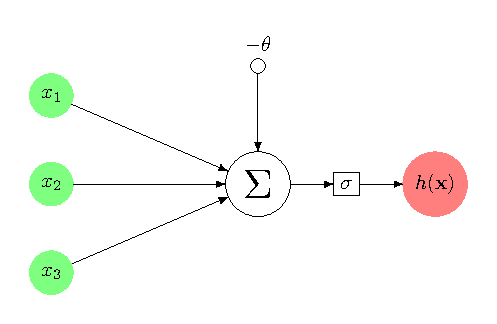
\includegraphics[width=.45\textwidth]{neuron-mp}
  \caption{Neurona McCulloch-Pitts con entrada $\textbf{x}$ y umbral $\theta$.}
  \label{fig:neuron-mp}
\end{figure}

\subsection{Perceptrón}

Con este modelo es posible representar alguna función muy sencilla pero no es útil para aprender funciones con un poco más de complejidad (observamos que el modelo está determinado por $\theta$, un único parámetro libre). Por ello surge una generalización de este modelo llamado el \textbf{perceptrón} \cite{rosenblatt1958perceptron}.

Este modelo incorpora una novedad fundamental: \textbf{pesos} que afectan a las entradas para regular las relaciones y las intensidades de estas. Al establecer conexiones más complejas entre las entradas se consigue que la neurona pueda aprender funciones que no sean tan simples como ocurría con la neurona de McCulloch-Pitts. También se admiten ahora las entradas reales, aumentando el dominio de entrada.

Definimos el perceptrón en \autoref{def:perceptron} y representamos visualmente en \autoref{fig:perceptron} viendo que lo que cambia simplemente son los pesos asociadas a las entradas, que actúan como reguladores de las conexiones.

\begin{definicion}[Perceptrón]
  Sea un vector de entrada $\textbf{x} \in \R^M$ con $M \in \N$, un vector de pesos $\textbf{w} \in \R^n$ y $\theta \in \R$ el umbral de activación, el perceptrón calcula la función $h$ dada por la siguiente expresión:

  $$h(\textbf{x}) = \sigma\left(\sum \limits^M_{i = 1}w_i x_i - \theta\right),$$

   donde $\sigma$ es la función de activación dada por $$\sigma(t) = \begin{cases} 1, \text{ si } t \geq 0 \\ 0, \text{ si } t < 0 \end{cases}.$$
   \label{def:perceptron}
\end{definicion}

\begin{figure}[htpb]
  \centering
  %\hspace*{-2.5cm}
  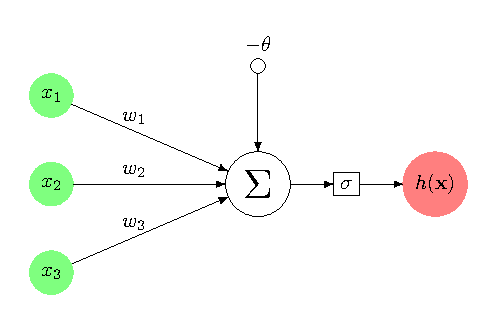
\includegraphics[width=.45\textwidth]{perceptron}
  \caption{Perceptrón con entrada $\textbf{x}$, pesos $\textbf{w}$ y umbral $\theta$.}
  \label{fig:perceptron}
\end{figure}

Considerando $\textbf{x} = (x_1, \ldots, x_M, 1)^T$ y $\textbf{w} = (w_1, \ldots, w_M, -\theta)^T$ podemos compactar la expresión, teniendo entonces $h(\textbf{x}) = \sigma(\textbf{w}^T \textbf{x})$. Observando detenidamente esta expresión vemos que lo que se tiene realmente es un modelo lineal: un \textbf{hiperplano} de $\R^{M}$ al que luego se le aplica una función no lineal.

Sabemos que un hiperplano divide $\R^{M}$ en dos regiones conexas, de manera que la función no lineal lo que está realizando realmente es asignar a cada región un valor distinto. Esta idea tan simple de funcionamiento nos permite pensar que el perceptrón sea capaz de solucionar \textbf{problemas de clasificación binarios}  (\autoref{def:clasbin}).

Estos problemas consisten fundamentalmente en inferir la relación que existe entre los datos de unas variables o \textbf{características} y las \textbf{etiquetas} asociadas a cada dato, que se identifican con una de las dos clases $+1$ o $-1$. Esta relación es la \textbf{función de etiquetado} desconocida $f$ que deseamos aprender, donde sabemos cómo se comporta en una \textbf{muestra} dada y que usaremos para que los modelos puedan aprender una función aproximada $h$. El objetivo entonces se convierte en conseguir que $h \approx f$ (ya veremos adelante como medimos esto).

Como nota adicional si consideramos la muestra extraída $(X, \textbf{y})$, podemos notar que $X \in \mathcal{M}_{N \times M}(\R)$ e $\textbf{y} \in \mathcal{M}_{N \times 1}(\N)$ y que

$$ X = \begin{bmatrix} \textbf{x}_1^T \\ \textbf{x}_2^T \\ \vdots \\ \textbf{x}_N^T \end{bmatrix}, \textbf{y} = \begin{bmatrix} y_1 \\ y_2 \\ \vdots \\ y_{N} \end{bmatrix}.$$

\begin{definicion}[Problema de clasificación binario]
  Sea $M \in \N$ el número de características, y $N \in N$ el número de observaciones, consideramos el espacio $\mathcal{X} \times Y \subseteq R^M \times \{-1, +1\}$ del que obtenemos una muestra $(X, \textbf{y}) \in \mathcal{X}^N \times Y^N$ que sigue una distribución de probabilidad $\mathcal{P}$ desconocida y el espacio de funciones del modelo dado $\mathcal{H}$. El problema consiste en encontrar un $h \in \mathcal{H}$ de tal manera que $h \approx f$, siendo $f$ la función de etiquetado:

  \begin{align*}
    f : \mathcal{X} & \to Y \\
    \textbf{x} & \mapsto f(\textbf{x}) \in \{-1, +1\}.
  \end{align*}
  \label{def:clasbin}
\end{definicion}

Sin más que cambiar los valores de la función de activación $\sigma$ de $\{0, 1\}$ a $\{-1, +1\}$ el perceptrón es capaz de aprender funciones capaces de solucionar estos problemas. De hecho, generalmente en el perceptrón se adopta en vez de la función $\sigma$ anteriormente comentada, la función $\sign$.

Podemos ver que el problema de clasificación binaria es equivalente a encontrar una función que separe dos conjuntos de datos agrupados por la clase, es decir a la separabilidad de dos conjuntos, que es lo que está haciendo el hiperplano $\textbf{w}$ del perceptrón (\autoref{fig:perceptron-ej} \cite{wikipedia2017separ}).

\begin{figure}[htpb]
  \centering
  %\hspace*{-2.5cm}
  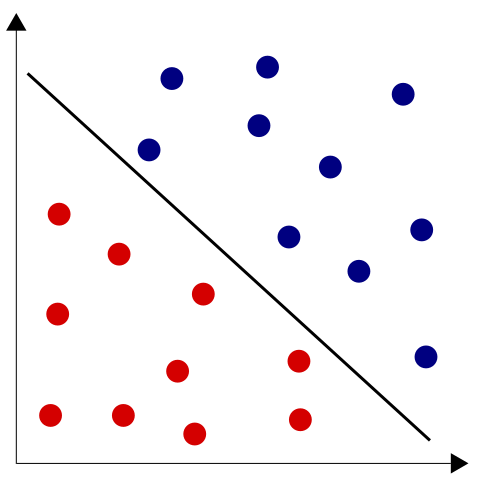
\includegraphics[width=.3\textwidth]{separabilidad}
  \caption{Ejemplo de perceptrón separando linealmente dos conjuntos de datos. Al separar es posible asignar a cada región una etiqueta, siendo equivalente separar a clasificar.}
  \label{fig:perceptron-ej}
\end{figure}

Gracias al Teorema de Convergencia del Perceptrón \cite{novikoff1963convergence} tenemos un resultado fuerte sobre la clase de funciones que puede aprender el perceptrón: se prueba que el modelo es capaz de aprender siempre una función $h$ que separa perfectamente dos conjuntos de datos que sean linealmente separables. Es decir, el perceptrón encuentra una solución muy buena $h \approx f$ ya que coinciden completamente, al menos en la muestra obtenida.

Mediante el \textbf{proceso de aprendizaje} se consigue que el modelo aprenda la función $h$ que buscamos. Este proceso es un método que tiene cada modelo de usar la información de la muestra recogida para poder aprender la función de etiquetado, que en el caso del perceptrón será una simple regla que actualiza los pesos por cada dato de la muestra \eqref{eq:percep-rule}.

\begin{equation}
  \textbf{w}_{(t + 1)} =
  \begin{cases}
    \textbf{w}_{(t)}, & \text{si } \sign(\textbf{w}^T_{(t-1)} \textbf{x}_t) \neq y_t \\
    \textbf{w}_{(t)} + y_t \textbf{x}_t, & \text{en caso contrario}
  \end{cases}.
  \label{eq:percep-rule}
\end{equation}

A pesar de todo, en cuanto los datos dejan de ser linealmente separables el perceptrón no tiene por qué converger siquiera a una solución. Si bien se puede arreglar quedándose con la mejor solución hasta el momento, las soluciones encontradas no suelen ser muy buenas. Por esta razón se necesitaba encontrar una manera de mejorar este modelo.

\subsection{Perceptrón MultiCapa}

Basándonos \cite{abu2012learning} explicaremos el proceso lógico que se lleva a cabo para poder aumentar la potencialidad del modelo del perceptrón.

Consideremos la siguiente función de la figura (\autoref{fig:xor}, \cite{abu2012learning}) que es bastante simple aunque la función $f$ no se puede aprender con un solo perceptrón (tomando una muestra se ve que los datos no son separables).

\begin{figure}[htpb]
  \centering
  %\hspace*{-2.5cm}
  \includegraphics[width=.35\textwidth]{XOR}
  \caption{Esta $f$ no se puede aprender con un solo perceptrón.}
  \label{fig:xor}
\end{figure}

Usemos dos perceptrones que aprendan cada uno de los hiperplanos separadores (\autoref{fig:dos-percep}, \cite{abu2012learning}) y fijémonos en las áreas de las clases. La función $f$ tiene la clase $+1$ cuando $h_1$ y $h_2$ tienen $(+1, -1)$ ó $(-1, +1)$; y la clase $-1$ cuando $(+1, +1)$ ó $(-1, -1)$. Este comportamiento es análogo a la función booleana $XOR$, por lo que podemos representarla como si lo fuera en base a las salidas de $h_1$ y $h_2$ ($f = XOR(h_1, h_2)$) siendo $+1$ \emph{Verdadero} y $-1$ \emph{Falso}. Usando notación booleana podemos reescribir $f = h_1\overline{h_2} + \overline{h_1}h_2$.

\begin{figure}[htpb]
  \centering
  %\hspace*{-2.5cm}
  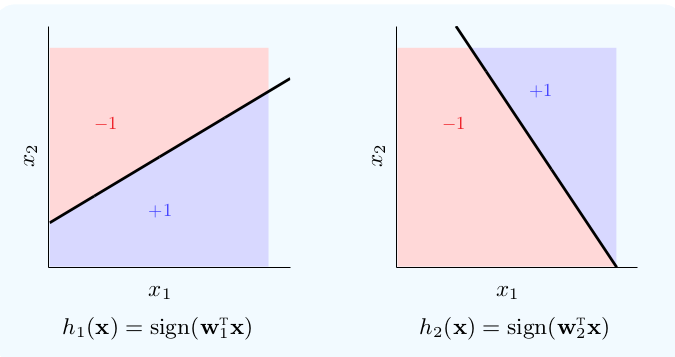
\includegraphics[width=.7\textwidth]{dospercep}
  \caption{Cada perceptrón aprende un hiperplano distinto.}
  \label{fig:dos-percep}
\end{figure}

Como estamos usando funciones $OR (+)$ y $AND (\cdot)$ para obtener $f$, el siguiente paso lógico es intentar expresar estas funciones como perceptrones. Es fácil ver que podemos obtenerlas de la siguiente manera \eqref{eq:and-or}.

\begin{align}
  AND(h1, h2) = \sign(h1 + h2 + 1.5), \\
  OR(h1, h2) = \sign(h1 + h2 - 1.5). \\
  \label{eq:and-or}
\end{align}

Representamos estas funciones en forma de perceptrones, considerando la forma compacta ($\textbf{x} = (x_1, \ldots, x_M, 1)$, $\textbf{w} = (w_1, \ldots, x_M, -\theta)$ que ya habíamos comentado con la Neurona de McCulloch-Pitts (\autoref{fig:and-or}, \cite{abu2012learning}).

\begin{figure}[htpb]
  \centering
  %\hspace*{-2.5cm}
  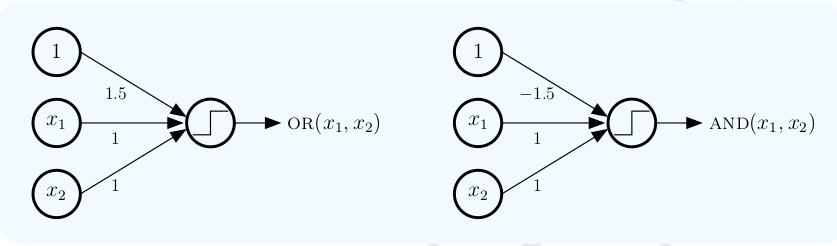
\includegraphics[width=.8\textwidth]{and-or}
  \caption{Funciones $AND$ y $OR$ como perceptrones.}
  \label{fig:and-or}
\end{figure}

Usando estos perceptrones podemos ir implementando poco a poco la función $f$: primero nos encontramos con una $OR$ que tiene como entradas $h_1\overline{h_2}$ y $\overline{h_1}h_2$ (\autoref{fig:or1}, \cite{abu2012learning}).

\begin{figure}[htpb]
  \centering
  %\hspace*{-2.5cm}
  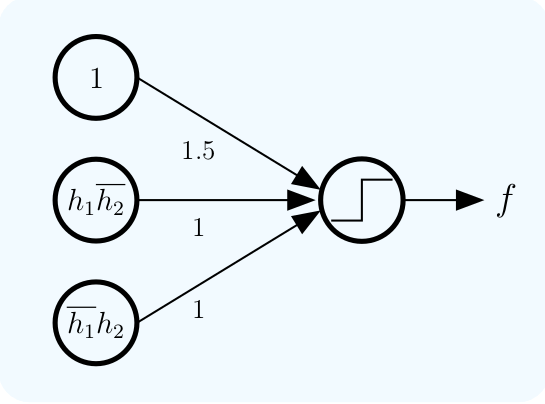
\includegraphics[width=.35\textwidth]{or1}
  \caption{Perceptrón que implementa $AND(h_1\overline{h_2}, \overline{h_1}h_2)$.}
  \label{fig:or1}
\end{figure}

Ahora tendríamos que usar dos perceptrones $AND$ para implementar $h_1\overline{h_2}$ y $\overline{h_1}h_2$. Como ambos perceptrones usarán la misma entrada ($\textbf{h} = (h_1, h_2, 1)$) se pueden representar los dos a la vez mediante dos vectores de pesos distintos (que son lo que determinan al perceptrón). Finalmente hay que tener en cuenta la negación de las entradas que se puede conseguir fácilmente cambiando el signo del peso asociado (\autoref{fig:and2}, \cite{abu2012learning}).

\begin{figure}[htpb]
  \centering
  %\hspace*{-2.5cm}
  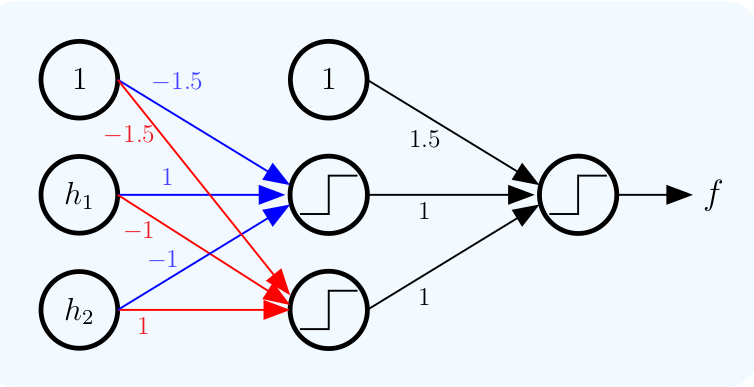
\includegraphics[width=.55\textwidth]{and2}
  \caption{Añadimos dos perceptrones $AND(h_1, \overline{h_2})$ (en azul) y $AND(\overline{h_1}, h_2)$ (en rojo).}
  \label{fig:and2}
\end{figure}

Falta obtener $h_1$ y $h_2$, pero si recordamos que se tenía que $h_1 = \sign(\textbf{w}^T_1 \textbf{x})$ y $h_2 = \sign(\textbf{w}^T_2 \textbf{x})$ que eran los dos perceptrones iniciales. Los incorporamos a nuestro esquema que ya estaría completo (\autoref{fig:mlp}, \cite{abu2012learning}).

\begin{figure}[htpb]
  \centering
  %\hspace*{-2.5cm}
  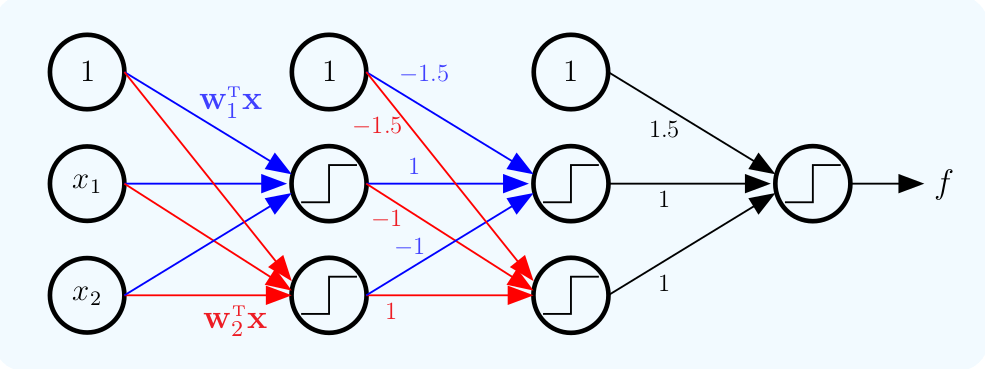
\includegraphics[width=.65\textwidth]{mlp}
  \caption{Los dos perceptrones iniciales $h_1$ (azul) y $h_2$ (rojo).}
  \label{fig:mlp}
\end{figure}

Analizando este modelo vemos que ha sido formado juntando perceptrones, uniendo las salidas de uno con la entrada de otro como si añadiésemos una \textbf{capa} tras otra de perceptrones. Debido a esto, este modelo se conoce como el \textbf{Perceptrón MultiCapa} (\emph{MultiLayer Perceptron}, MLP) \cite{rumelhart1985learning} y es de hecho la primera estructura de red neuronal básica y sobre la que se vertebrará toda la estructura del aprendizaje profundo.

\section{Redes Neuronales Hacia Adelante}

\subsection{Descripción}

Estudiamos las \textbf{redes neuronales hacia delante} (\emph{feedforward neural networks}, FFNN) que son las estructuras de redes neuronales más básicas y funcionales, donde sus procesos de funcionamiento y aprendizaje son el núcleo central de las redes neuronales, por lo que al estudiarlos en detalle nos permitirán entender \emph{a grosso modo} cualquier arquitectura utilizada actualmente.

Como hemos visto, este modelo surge con el perceptrón multicapa que se puede considerar un caso particular de esta aunque también se puede denominar como el mismo tipo de red. Usaremos como base los resultados y explicaciones de \cite{abu2012learning} para detallar exhaustivamente comentando su estructura, algoritmos de cómputo y aprendizaje.

\begin{figure}[htpb]
  \centering
  %\hspace*{-2.5cm}
  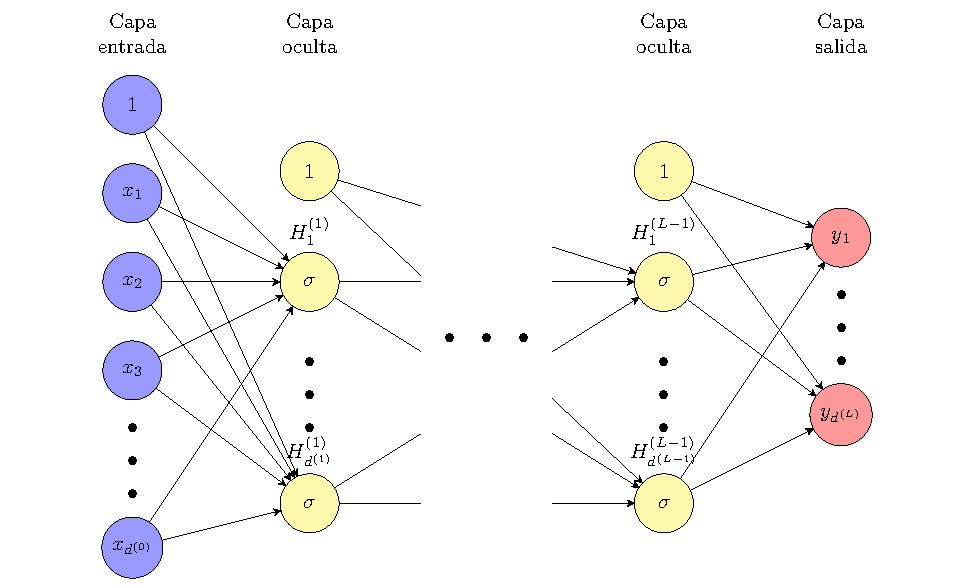
\includegraphics[width=1.\textwidth]{ffnn}
  \caption{Estructura genérica de una FFNN con $L$ capas, dimensiones $d^{(\ell)}$, entrada $\textbf{x}$, salida $\textbf{y}$ y funciones de activación $\sigma$.}
  \label{fig:ffnn}
\end{figure}

\subsection{Estructura}

\subsubsection{Arquitectura}

Veamos primero una estructura general de ejemplo en \autoref{fig:ffnn}. Consideramos una red con $L$ capas, etiquetadas con $\ell = 0, 1, \ldots, L$ donde $\ell = 0$ se corresponde con la capa de \textbf{entrada}, de las variables, que no se suele contar como una capa propia por lo que cuando se dice que una red tiene $L$ capas estamos diciendo que tiene $L-1$ capas intermedias ($0 < \ell < L$), llamadas capas \textbf{ocultas} y la capa $\ell = L$ de \textbf{salida} que es el resultado de la red.

Cada capa tiene una dimensión concreta, que denotaremos por $d^{(\ell)}$ y que indica que la capa $\ell$ tiene $d^{(\ell)} + 1$ nodos o neuronas (incluimos el nodo 1 del sesgo $\theta$) excepto para la capa de salida que se puede obviar. En particular se tiene que $d^{(0)} = M$, el número de variables y que $d^{(L)}$ será la dimensión de la salida, que ya no tiene que ser obligatoriamente un único nodo; de hecho, la salida ya no tiene que tomar valores discretos ya que podemos considerar otras funciones de activación que veremos un poco más adelante.

Observando este diagrama en profundidad notamos que cada neurona de una capa estará conectada por un peso (las conexiones) a todas las neuronas de la siguiente capa, formándose una red \textbf{densa}, nombre por la que también se suele conocer este tipo de capa. Esta estructura de conexiones de entrada a salida, capa por capa, es lo que le da nombre a este tipo de red puesto que los resultados se van pasando \emph{hacia adelante} siempre.

Adicionalmente, tengamos que en cuenta que si cada neurona está asociada con unos pesos, toda la capa $\ell$ que está formada por $d^{(\ell)}$ (sin contar la de sesgo) estará determinada por todos los pesos de cada neurona, que podemos representar como una matriz \eqref{eq:pesos}.

\begin{equation}
  W^{(\ell)} = \begin{bmatrix} \textbf{w}^{(\ell)}_{1} \ldots \textbf{w}^{(\ell)}_{d^{(\ell)}} \end{bmatrix} \in \mathcal{M}_{(d^{(\ell - 1)} + 1) \times d^{(\ell)}}(\R).
  \label{eq:pesos}
\end{equation}

\subsubsection{Función de activación}

Respecto las funciones de activación $\sigma$, también llamadas funciones \textbf{de transformación} ya que son funciones no lineales, se deja de usar la función $\sign()$ en las capas ocultas debido a su discontinuidad en pos de otras funciones aproximadas más \emph{suaves} que realizan una función igual o muy parecida; las más famosas y usadas son las siguientes (funciones dibujadas \autoref{fig:activations}, \cite{moujahid2016activations}):

\begin{enumerate}
  \item Sigmoide: $$\sigma(x) = \dfrac{1}{1 + e^{-x}}.$$
  \item Tangente hiperbólica: $$\tanh(x) = \dfrac{e^x-e^{-x}}{e^{x}+e^{-x}}.$$
  \item ReLU (REctifier Linear Unit): $$ReLU(x) = x^+ = max(0, x).$$
\end{enumerate}

\begin{figure}[htpb]
  \centering
  %\hspace*{-2.5cm}
  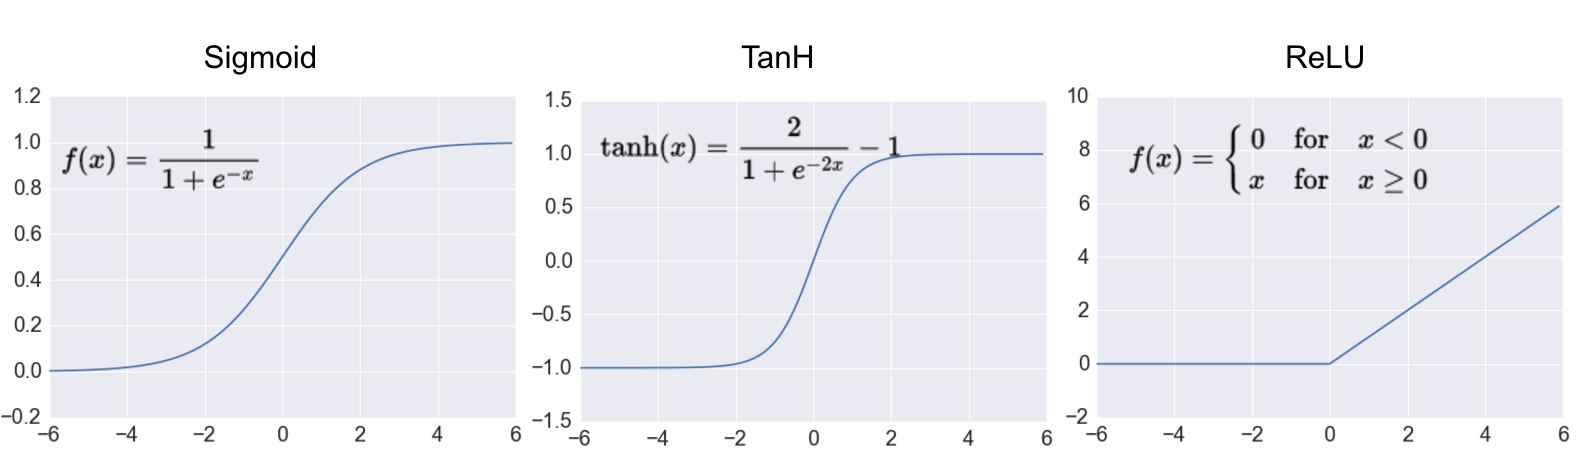
\includegraphics[width=1.\textwidth]{activations}
  \caption{Funciones de activación.}
  \label{fig:activations}
\end{figure}

Donde sí podremos usar $\sign()$ será en la capa de salida cuando queramos obtener un resultado respecto una clase, sin embargo recordemos que ahora podemos tener una dimensión de salida cualquiera y no estamos limitados a aprender funciones discretas. De hecho, si consideramos otras capas de activación para la salida podemos aprender distintos tipos de funciones según el problema que tengamos entre manos.

Por ejemplo, para los problemas de \textbf{regresión} que son simplemente problemas de clasificación donde la $f$ pasa de ser discreta a continua ($f: \mathcal{X} \to Y$, $Y \subseteq \R^n$) podemos usar directamente la función identidad ($f(x) = x$); para los problemas de \textbf{regresión logística}, que considera una función que en vez de asignar una clase directamente asigna la \textbf{probabilidad} ($\mathcal{X} \to Y$, $Y \subseteq [0, 1]$), se puede usar la función $\tanh()$ o \emph{sigmoide}.

De hecho, cuando tenemos un problema de clasificación con $n$ clases en vez de calcular una clase directamente se calcula la probabilidad \textbf{asociada} a cada clase y cuando se hace una clasificación de una única clase se toma la de mayor probabilidad. Esto es posible utilizando en la capa de salida la función de activación \textbf{softmax} \autoref{def:softmax}, que toma un vector real de tamaño $n$ y lo normaliza en una distribución de probabilidad.

\begin{definicion}[Softmax]
  La función softmax es una función $\sigma : \R^n \to \R^n$ definida de la siguiente forma:
  $$\sigma(\textbf{x}) = \sum \limits^n_{i = 1} e^{x_i} \begin{pmatrix} e^{x_1} \\ \vdots \\ e^{x_n}\end{pmatrix}.$$
  \label{def:softmax}
\end{definicion}

En cualquier caso, el modelo $\mathcal{H}_{nn}$ queda determinado por la \textbf{arquitectura} de la red neuronal, es decir, especificar el número de capas y la dimensión de cada capa: fijar $L$ y $\textbf{d} = [d^{(0)}, d^{(1)}, \ldots, d^{(L)}]$. Por tanto cada función de hipótesis $h \in \mathcal{H}_{nn}$ estará representada por los pesos de las conexiones entre las capas que representaremos con matrices: $\textbf{W} = \{W^{(1)}, W^{(2)}, \ldots, W^{(L)}\}$.

\subsection{Propagación hacia adelante}

Antes de explicar el algoritmo de cálculo de $h(\textbf{x})$, indiquemos una breve notación: sea $\ell \in \{1, 2, \ldots, L\}$, consideramos la capa $\ell$ que recibe el el resultado $\textbf{s}^{(\ell)} \in \mathcal{M}_{d^{(\ell)} \times 1}(\R)$ de la multiplicación de la capa anterior \eqref{eq:fp1} de los datos de entrada $\textbf{x}^{(\ell-1)} \in \mathcal{M}_{(d^{(\ell-1)} + 1) \times 1}(\R)$ con los pesos $W^{(\ell)} \in \mathcal{M}_{(d^{(\ell-1)} + 1) \times d^{(\ell)}}(\R)$

\begin{equation}
  \textbf{s}^{(\ell)} = (W^{(\ell)})^T \textbf{x}^{(\ell-1)},
  \label{eq:fp1}
\end{equation}

a los que le aplica la función de activación $\sigma$ obteniendo la salida $\textbf{x} \in \mathcal{M}_{d^{(\ell) \times 1}}(\R)$ \eqref{eq:fp2}

\begin{equation}
  \textbf{x}^{(\ell)} = \begin{bmatrix} 1 \\ \sigma(\textbf{s}^{(\ell)})\end{bmatrix}.
  \label{eq:fp2}
\end{equation}

La \textbf{propagación hacia adelante} (\emph{forward propagation}) es el algoritmo para poder calcular el resultado de la red $h(\textbf{x})$. A partir de los datos de entrada $\textbf{x}^{(0)}$ se calcula la siguiente salida de la capa que se \textbf{propaga} a la siguiente capa y así hasta llegar al final siguiendo la siguiente cadena \eqref{eq:cadena-fp}

\begin{equation}
  \textbf{x} = \textbf{x}^{(0)} \xrightarrow[]{W^{(1)}} \textbf{s}^{(1)} \xrightarrow[]{\sigma} \textbf{x}^{(1)} \xrightarrow{W^{(2)}} \ldots \xrightarrow{\sigma} \textbf{x}^{(L)} = h(\textbf{x}).
  \label{eq:cadena-fp}
\end{equation}

Formalizamos este proceso mediante el algoritmo \autoref{alg:fp} \cite{abu2012learning}. Aunque en principio solo necesitamos la última salida $h(\textbf{x}) = \textbf{x}^{(L)}$ devolvemos todas las entradas $\textbf{x'}$ y salidas $\textbf{s}$ ya que los necesitaremos más adelante.

\begin{algorithm}[htbp]
\SetAlgoLined
 \tcp{Inicializamos con la entrada}
 $\textbf{x}^{(0)} \gets \textbf{x}$\;
 \tcp{Propagamos para cada capa}
 \For{$\ell = 1, \ldots, L$} {
  \tcp{Calculamos la entrada de la capa}
  $\textbf{s}^{(\ell)} \gets (W^{(\ell)})^T \textbf{x}^{(\ell - 1)}$\;
  \tcp{Se devuelve la salida de la capa}
  $\textbf{x}^{(\ell)} \gets \begin{bmatrix} 1 \\ \sigma(\textbf{s}^{(\ell)})\end{bmatrix}$\;
 }
 \tcp{Devolvemos las entradas y salidas}
 $\textbf{x'} \gets \left[\textbf{x}^{(0)}, \ldots, \textbf{x}^{(L)}\right]$\;
 $\textbf{s} \gets \left[\textbf{s}^{(1)}, \ldots, \textbf{s}^{(L)}\right]$\;
 \KwResult{$\textbf{x'}$, $\textbf{s}$}
 \caption{$ForwardPropagation(\textbf{x})$)}
 \label{alg:fp}
\end{algorithm}

\subsection{Descenso en gradiente}

Lo último que nos falta para poder empezar a usar estos modelos es un mecanismo de aprendizaje, el algoritmo para que la red pueda aprender la función $f$ mediante la muestra de datos que tenemos, es decir buscar una $h \in \mathcal{H}_{nn}$ tal que $h \approx f$, o lo que es lo mismo $h(\textbf{x}) \approx f(\textbf{x}), \; \forall \textbf{x} \in \mathcal{X}$.

Está claro que cuanto más se aproxime $h$ a $f$ mejor será, aunque necesitamos una manera de formalizar esta similitud para poder trabajarla. Recordemos que tenemos una muestra que podemos suponer que es suficientemente grande y representativa de la distribución subyacente que se puede usar para poder valorar la diferencia entre $h$ y $f$. La idea que surge es valorar con una función de \textbf{error} o \textbf{pérdida} las diferencias entre $f$ y $h$ para todos los valores de la muestra, dando un valor indicativo con el que podemos trabajar.

Este tipo de funciones generalmente son de la forma $E_{\mathcal{D}} : \mathcal{H} \to \R^+_0$ que toman una función del conjunto de hipótesis del modelo y se valora en base a un criterio impuesto según el problema que se quiera resolver usando la muestra $\mathcal{D}$; por ejemplo para problemas de regresión uno querría usar el conocido \textbf{error cuadrático medio}. Fijando una función de error, como queremos la función $h$ que menor $E_{\mathcal{D}}(h)$ tenga el problema de aprendizaje se ha convertido en un problema de \textbf{minimización}, teniendo en cuenta que para que la función sea de variable real tomaremos la representación de $h$ por los pesos $\textbf{w}$ (veremos cómo extenderlo a $\textbf{W}$).

Es importante entender que se puede imponer una función de error para minimizar en un modelo pero que luego el problema original que se quiere resolver sea distinto, de manera que la \textbf{valoración} del modelo se realizará de otra manera; concretamente usaremos las \textbf{métrica} para valorar la bondad de los modelos, que veremos con detalle más adelante en \autoref{ch:metricas}.

Nuestro problema de aprendizaje se ha convertido en un problema de minimización donde para resolverlo podemos recurrir a los métodos numéricos existentes como el \textbf{Descenso en Gradiente} (\emph{Gradient descent}, GD). \cite{curry1944method}.

El descenso en gradiente (\autoref{def:gd}) es un método de minimización cuya idea principal se basa en ir moviéndose hacia el mínimo \emph{bajando} poco a poco tomando la dirección contraria (negativa) del gradiente (\autoref{fig:gd}, \cite{molala2019sd}). Como la dirección del gradiente indica donde aumenta la función localmente, al tomar la dirección contraria después de suficientes iteraciones, esperamos idealmente llegar al menos a un mínimo local (pudiera acabar en puntos de silla) aunque lo deseable será llegar al global si lo hubiera. Bajo ciertas condiciones podemos asegurar la convergencia de este método, por ejemplo si la función es convexa y el gradiente es lipschiziano \cite{shalev2014understanding}.

\begin{figure}[htpb]
  \centering
  %\hspace*{-2.5cm}
  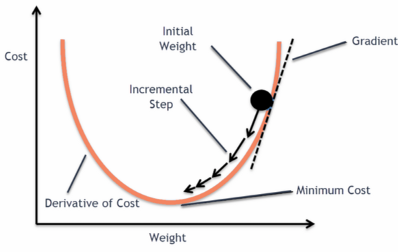
\includegraphics[width=.5\textwidth]{gd}
  \caption{Ejemplo del Descenso en Gradiente en una parábola.}
  \label{fig:gd}
\end{figure}

\begin{definicion}[Descenso en grandiente]
  Sea $E : \R^m \to \R$ una función diferenciable, un punto inicial $\textbf{w}_{(0)}$ y la tasa de aprendizaje $\mu \in \R^+$. El descenso en gradiente es un método iterativo de primer orden para encontrar mínimos que sigue la siguiente regla de actualización:

  $$\textbf{w}_{(t)} = \textbf{w}_{(t-1)} - \mu \nabla E(\textbf{w}_{(t-1)}), \; \forall t \in \N.$$
  \label{def:gd}
\end{definicion}

El establecer un valor para la \textbf{tasa de aprendizaje} (\emph{learning rate}) no es una tarea para nada trivial, de hecho en \autoref{fig:lr} podemos ver las implicaciones de no escoger una tasa adecuada: si es muy baja puede resultar en una convergencia \textbf{muy lenta}, y si es alta puede que \textbf{no converga} o lo haga saltándose mínimos \textbf{mejores}, también podría pasar que el error \emph{explote} (diverge) \cite{ruder2016overview}.

\begin{figure}[htpb]
  \centering
  %\hspace*{-2.5cm}
  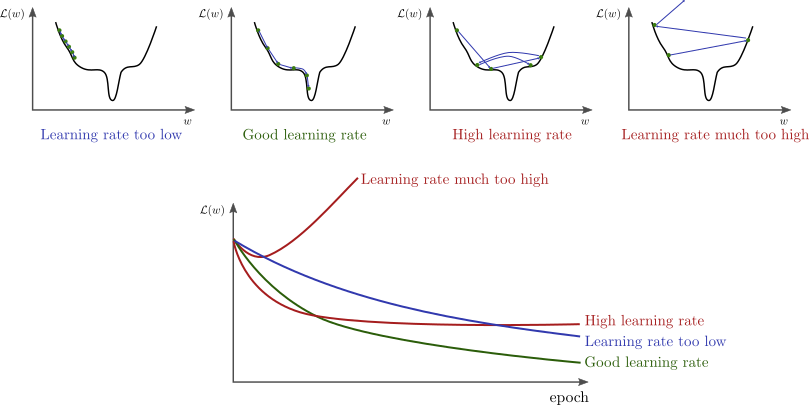
\includegraphics[width=.9\textwidth]{lr}
  \caption{Diferentes resultados según la tasa de aprendizaje $\mu$.}
  \label{fig:lr}
\end{figure}

En principio ya tendríamos un método para poder intentar que nuestra red pueda aprender pero tenemos un problema general a la hora de calcular $\nabla E_\mathcal{D}$: si nuestra muestra de datos $\mathcal{D}$ es muy grande esto puede provocar que el cálculo sea muy costoso en tiempo e incluso supere los tamaños de memoria del \emph{hardware} y esto solo para un paso, por lo que para realizar las múltiples iteraciones necesarias para la convergencia resulte completamente inviable \cite{ruder2016overview}.

La solución a esto la aporta el \textbf{Descenso en Gradiente Estocástico} (\emph{Stochastic Gradient Descent}, SGD) \cite{robbins1951stochastic} que es igual que el Descenso en Gradiente, solo que en vez de tomar todo el conjunto de datos de golpe $\mathcal{D}$ se hace una partición en subconjuntos de tamaño $n$ llamados \textbf{lotes} o \emph{batches} y se actualizan los pesos para cada \emph{batch}. La aleatoriedad que se introduce al escoger los \emph{batches} es interesante ya que nos puede ayudar en la búsqueda de mínimos, aportándonos un poco de exploración para encontrar mejores mínimos en la función.

Técnicamente se llama SGD cuando $n=1$, es decir, cuando actualizamos la red dato a dato, cuando $1 < n < N$ se suele llamar al método \textbf{Descenso en Gradiente con Mini-lotes} (\emph{Mini-batch Gradient Descent}) aunque también se usa SGD indistintivamente.

Respecto al tamaño del \emph{batch} $n$, el rango de valores típico de suele estar en $[32, 256]$ aunque dependerá del modelo y problema concretos que se esté considerando, se suele probar con los valores típicos y se van adaptando para obtener un buen funcionamiento.

En principio ya estaríamos listos para que nuestra red aprendiera, pero merece la pena mencionar que en la actualidad se utilizan métodos derivados más complejos que intentan mejorar el funcionamiento del SGD para una convergencia más rápida y encontrar mejores mínimos. Listamos unos cuantos de los más conocidos y populares: \textbf{Adadelta}, \textbf{RMSprop}, \textbf{Adam}, \textbf{AdaMax} y \textbf{Nadam} \cite{ruder2016overview}. No existe un método absoluto que gane a todos, de hecho SGD sigue siendo una opción viable, por lo que dependiendo del problema se puede decidir escoger uno y otro; aun así uno de los optimizadores más populares y que se suele escoger para las redes neuronales es \textbf{Adam}.

\subsection{Propagación hacia atrás}

\subsubsection{Sensibilidades}

Vamos a aplicar SGD para que nuestro modelo aprenda, para ello necesitamos $\nabla E_{\mathcal{D}} (\textbf{w})$ pero aquí $\textbf{w} = \{W^{(1)}, \ldots, W^{(L)}\}$ por lo que hay que calcular las derivadas parciales respecto \textbf{todas las matrices}. Considerando que el error en la muestra no es más que la media de los errores de cada dato podemos reescribir como \eqref{eq:esample}

\begin{equation}
  E_{\mathcal{D}}(\textbf{w}) = \dfrac{1}{N} \sum \limits_{d \in \mathcal{D}} E_d(\textbf{w}) = \dfrac{1}{N} \sum \limits^N_{i = 1} e_i.
  \label{eq:esample}
\end{equation}

Y por tanto las derivadas parciales del error respecto cada matriz de $\textbf{w}$ serán como \eqref{eq:ederiv}

\begin{equation}
  \dfrac{\partial E_{\mathcal{D}}}{\partial W^{(\ell)}} = \dfrac{1}{N} \sum \limits^N_{i = 1} \dfrac{\partial e_i}{\partial W^{(\ell)}}.
  \label{eq:ederiv}
\end{equation}

Es posible usar métodos numéricos para obtener cada $\dfrac{\partial e}{\partial W^{(\ell)}}$ pero la complejidad del algoritmo para la derivada respecto cada peso sería de $O(Q^2)$ siendo $Q$ el número de pesos, que se hace computacionalmente inviable. Surge así el algoritmo de la \textbf{propagación hacia atrás} (\emph{backpropagation}) que nos permite calcular estas derivadas eficientemente con una complejidad de $O(Q)$.

Este algoritmo se basa en la \textbf{regla de la cadena} para expresar las derivadas parciales de la capa $\ell$ en base a las de la capa $(\ell + 1)$. Para describir el funcionamiento, definamos primero el \textbf{vector de sensibilidad} (\autoref{def:sensibilidad}) que trata de medir como cambia $e$ respecto $\textbf{s}^{\ell}$.

\begin{definicion}[Vector de sensibilidad]
  Sea $\ell \in \N$, el vector de sensibilidad de la capa $\ell$ notado por $\pmb{\delta}^{(\ell)}$, es el gradiente del error $e$ respecto la señal de entrada en la capa $\textbf{x}^{(\ell)}$, es decir:

  $$\pmb{\delta}^{(\ell)} = \dfrac{\partial e}{\partial \textbf{s}^{(\ell)}}.$$
  \label{def:sensibilidad}
\end{definicion}

Usando la regla de la cadena, y recordando que $\textbf{s}^{(\ell)} = (W^{(\ell)})^T \textbf{x}^{(\ell-1)}$ expresamos las derivadas parciales con la sensibilidad \eqref{eq:senpar} \cite{abu2012learning}

\begin{equation}
  \dfrac{\partial e}{\partial W^{(\ell)}} = \dfrac{\partial e}{\partial \textbf{s}^{(\ell)}} \cdot \dfrac{\partial \textbf{s}^{(\ell)}}{\partial W^{(\ell)}} = \textbf{x}^{(\ell - 1)}(\pmb{\delta}^{(\ell)})^T.
  \label{eq:senpar}
\end{equation}

Además, considerando que $\textbf{x}^{(\ell)} = \sigma(\textbf{s}^{(\ell)})$ y volviendo a aplicar la regla de la cadena podemos obtener la sensibilidad de la capa $(\ell)$ en función de la de $(\ell + 1)$ para cada coordenada \eqref{eq:senpar2}, que extendemos al vector entero \eqref{eq:senpar3} \cite{abu2012learning}

\begin{equation}
  \delta_i^{(l)} = \dfrac{\partial e}{\partial s_i^{(l)}} =  \sum \limits^{d^{(\ell)}}_{j = 1} \left(\dfrac{\partial e}{\partial s_j^{(\ell + 1)}} \cdot \dfrac{\partial s_j^{(\ell + 1)}}{\partial x_i^{(\ell)}} \right) \cdot \dfrac{\partial x_i^{(\ell)}}{\partial s_i^{(\ell)}} = \sum \limits^{d^{(\ell)}}_{j = 1} \left(\delta^{(\ell)}_i w_{ij}^{(\ell)}\right) \sigma'(s_i^{(\ell)}),
  \label{eq:senpar2}
\end{equation}

\begin{equation}
  \pmb{\delta}^{(\ell)} = \sigma'(\textbf{s}^{(\ell)}) \otimes \left[W^{(\ell + 1)} \pmb{\delta}^{(\ell + 1)}\right]^{d^{(\ell)}}_1.
  \label{eq:senpar3}
\end{equation}

$\otimes$ denota la multiplicación componente a componente y $\left[\empty\textbf{v}\right]^{d^{(\ell)}}_{1}$ indica que se toman las componentes $1, \ldots, d^{(\ell)}$ del vector $\textbf{v}$ que simplemente indica que no contamos la componente del nodo de sesgo (el nodo 1).

Recapitulando: las salidas $\textbf{x}^{(\ell)}$ se pueden obtener simplemente calculando el resultado de la red (propagación hacia adelante), lo que resta por calcular son las sensibilidades $\pmb{\delta}^{(\ell)}$. Replicamos el algoritmo de la propagación hacia adelante con modificaciones: en vez de ir obteniendo y propagando las salidas hacia adelante (se usa $\textbf{x}^{(\ell)}$ para $\textbf{x}^{(\ell + 1)}$), lo haremos con las sensibilidades propagándolas \emph{hacia atrás} (se usa $\pmb{\delta}^{(l+1)}$ para $\pmb{\delta}^{(\ell)}$).

Empezaremos calculando $\pmb{\delta}^{(L)}$ directamente con la definición y después iremos propagando hacia atrás las sensibilidades. Por ejemplo, si consideramos el error cuadrático medio con un modelo cuya salida sea un único valor tendríamos $e(\textbf{x}; h) = (h(\textbf{x}) - y)^2$ y podemos calcular la sensibilidad fácilmente \eqref{eq:delta-ele}

\begin{equation}
  \pmb{\delta}^{(L)} = \dfrac{\partial e}{\partial \textbf{s}^{(L)}} = \dfrac{\partial}{\partial \textbf{s}^{(L)}} (\textbf{x}^{(L)} - y)^2 = 2(\textbf{x}^{(L)} - y) \dfrac{\partial \textbf{x}^{(L)}}{\partial \textbf{s}^{(L)}} = 2(\textbf{x}^{(L)} - y)\sigma'(\textbf{s}^{(L)}).
  \label{eq:delta-ele}
\end{equation}

Después habrá que calcular la derivada de la función de activación elegida, por ejemplo para $\sigma(s) = \tanh(s)$ tenemos que $\sigma'(\textbf{s}^{(L)}) = 1 - \sigma(\textbf{s}^{(L)})^2$; para la lineal (la identidad) $\sigma(\textbf{s}^{(L)}) = \textbf{s}^{(L)}$ se tendrá simplemente que $\sigma'(\textbf{s}^{(L)}) = 1$.

Describimos el método de \emph{backpropagation} por el cual calculamos las sensibilidades $\pmb{\delta}^{(\ell)}$ en \autoref{alg:bp}.

\begin{algorithm}[htbp]
\SetAlgoLined
 \tcp{Hacemos propagación hacia adelante para obtener $\textbf{x}$ y $\textbf{s}$}
 $\left[\textbf{x}^{(0)}, \ldots, \textbf{x}^{(L)}\right], \left[\textbf{s}^{(1)}, \ldots, \textbf{s}^{(L)}\right] \gets ForwardPropagation(\textbf{x})$\;
 \tcp{Inicializamos las sensibilidades}
 $\pmb{\delta} \gets \dfrac{\partial e}{\partial \textbf{s}^{(L)}}(\textbf{x}, y)$\;
 \tcp{Propagamos hacia atrás}
 \For{$\ell = L-1, \ldots, 1$} {
  \tcp{Calculamos la sensibilidad}
  $\pmb{\delta}^{(\ell)} \gets \sigma'(\textbf{s}^{(\ell)}) \otimes \left[W^{(\ell + 1)}\pmb{\delta}^{(\ell + 1)}\right]^{d^{(\ell)}}_1$
 }
 \tcp{Devolvemos las sensibilidades}
 $\pmb{\delta} \gets \left[\pmb{\delta}^{(1)}, \ldots, \pmb{\delta}^{(L)}\right]$\;
 \KwResult{$\pmb{\delta}$}
 \caption{$BackPropagation(\textbf{x}, y)$}
 \label{alg:bp}
\end{algorithm}

\subsubsection{Aprendizaje}

Por fin podemos definir el algoritmo SGD \autoref{alg:sgd-nn} por el cual podemos hacer que la red aprenda: solo necesitamos pasar como parámetros la muestra $(X, \textbf{y})$, la tasa de aprendizaje $\mu$ y el tamaño de los mini-\emph{batches} $tam_{batch}$. Obviamente se habrá fijado la arquitectura de la red junto a la función de error a minimizar y las funciones de activación.

\begin{algorithm}[htbp]
\SetAlgoLined
  \tcp{Inicializamos los pesos aleatorios}
  $\left[ W^{(1)}, \ldots, W^{(L)}\right] \gets PesosAleatorios()$\;
  \tcp{Iteramos hasta que se cumpla el criterio de parada}
  \Repeat{$CondicionParada()$}{
    \tcp{Dividimos aleatoriamente en mini-\emph{batches} de tamaño $tam_{batch}$}
    $n_{batches} \gets M \, // \, tam_{batch}$\;
    $\left[(X_{1}, \textbf{y}_1), \dots, (X_{n_{batches}}, \textbf{y}_{n_{batches}})\right] \gets ParticionAleatoria(X, \textbf{y})$\;
    \tcp{Por cada mini-\emph{batch} actualizamos los pesos}
    \For{$i = 1, \ldots, n_{batches}$}{
      \tcp{Inicializamos los gradientes a 0}
      $\left[G^{(\ell)}, \ldots, G^{(L)}\right] \gets 0 \cdot \left[W^{(1)}, \ldots, W^{(L)}\right]$\;
      \tcp{Calculamos el gradiente de todo el mini-\emph{batch}}
      \For{$(\textbf{x}, y) \in (X_{i}, \textbf{y}_i)$}{
        \tcp{Forwardpropagation y backpropagation}
        $\left[\textbf{x}^{(0)}, \ldots, \textbf{x}^{(L)}\right] \gets ForwardPropagation(\textbf{x})$\;
        $\left[\pmb{\delta}^{(1)}, \ldots, \pmb{\delta}^{(L)}\right] \gets BackPropagation(\textbf{x}, y)$\;
        \tcp{Actualizamos el gradiente de cada capa}
        \For{$\ell = 1, \ldots, L$}{
          $G^{(\ell)}(\textbf{x}) \gets \textbf{x}^{(\ell-1)}(\pmb{\delta}^{(\ell)})^T$\;
          $G^{(\ell)} \gets G^{(\ell)} + \dfrac{1}{tam_{batch}}G^{(\ell)}(\textbf{x})$\;
        }
      }
      \tcp{Actualizamos los pesos de cada capa}
      \For{$\ell = 1, \ldots, L$}{
        $W^{(\ell)} \gets W^{(\ell)} - \mu G^{(\ell)}$\;
      }
    }
  }
 \tcp{Devolvemos los pesos}
 $\textbf{w} \gets \left[ W^{(1)}, \ldots, W^{(L)}\right]$\;
 \KwResult{$\textbf{w}$}
 \caption{$AprendizajeRed(X, \textbf{y}, \mu, tam_{batch})$}
 \label{alg:sgd-nn}
\end{algorithm}

Esta es la base completa de las redes neuronales, las distintas arquitecturas que se han desarrollado a lo largo de los últimos años no cambian demasiado en los aspectos fundamentales por lo que sabiendo todo lo que hemos visto podemos hacernos una idea de cómo se extiende a los casos más complejos.

\subsection{Error y sobreajuste}

También tenemos que comentar que a la hora de entrenar las redes neuronales hay que tener en cuenta un aspecto fundamental en el aprendizaje automático: el \textbf{compromiso} entre el \textbf{sesgo} (\emph{bias}) y la \textbf{varianza} (\emph{variance}).

Cuando hablamos de sesgo estamos generalmente hablando del error del modelo en el conjunto de nuestra muestra, notado típicamente por $E_{in}$ y en principio es el error que queremos reducir en el proceso de aprendizaje de nuestros modelos. Sin embargo tenemos un problema, si intentamos ajustarnos perfectamente a los datos casi anulando efectivamente el sesgo pudiera ser que en otra muestra distinta de datos observemos que el modelo no ajusta bien estos nuevos datos.

Este efecto es el conocido \textbf{sobreajuste} (\emph{overfitting}) que se da cuando el error de entrenamiento $E_{in}$ no coincide (generalmente es mucho más bajo) con $E_{out}$ que es el error del modelo fuera de nuestra muestra. Este efecto ocurre debido al término de la \textbf{varianza} del error, que para nuestro modelo probablemente sea muy alta, y que nos indica generalmente el grado de variabilidad del error para una muestra distinta de datos.

Cuanto más queramos bajar el sesgo, más nos ajustaremos a los datos y provocaremos que aumente la varianza y por tanto tengamos sobreajuste; si no bajamos el sesgo a costa de no aumentar la varianza entonces el modelo pudiera estar mal ajustado (\emph{underfitting}). Tenemos que encontrar un \textbf{compromiso} entre ambos términos, un equilibrio adecuado para poder alcanzar un buen modelo que resuelva nuestro problema; podemos ver un ejemplo de lo que hablamos en una problema de regresión \autoref{fig:overfitting} \cite{bhande2018overfitting}.

\begin{figure}[htpb]
  \centering
  %\hspace*{-2.5cm}
  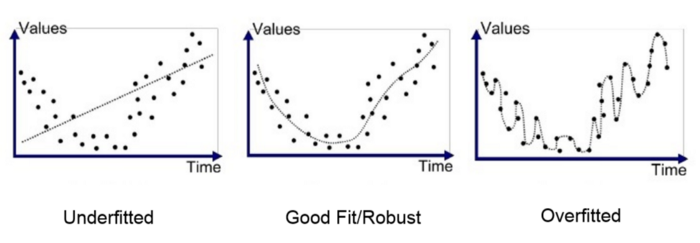
\includegraphics[width=.9\textwidth]{overfitting}
  \caption{Efecto del \emph{overfitting} y \emph{underfitting}.}
  \label{fig:overfitting}
\end{figure}

El proceso del sobreajuste está relacionado con la \textbf{complejidad} del modelo, que nos indica la capacidad del conjunto de hipótesis $\mathcal{H}$ para aprender funciones, siendo una medida común
la \textbf{Dimensión de Vapnik-Chervonenkis} (dimensión VC) $d_{VC}$ \cite{vapnik2015uniform}.  La idea principal es que cuanto más alta es esta dimensión, el modelo es capaz de aprender funciones más complejas y por tanto es capaz de ajustar bien los datos; sin embargo si la complejidad es mucho mayor que la de la función entonces es cuando se produce el efecto del sobreajuste.

Para evitar esto utilizamos técnicas de \textbf{regularización} que se encargan de imponer condiciones sobre el modelo reduciendo así el conjunto de hipótesis $\mathcal{H}$ considerado y disminuyendo su complejidad, que se traduce a un decremento de la varianza a costa de un pequeño aumento del sesgo.

Dentro de este campo hay muchas técnicas que podemos aplicar a las redes neuronales: reducción de la dimensión en profundidad y/o anchura, parada temprana (\emph{early stopping}) que trata de parar el entrenamiento bajo ciertas condiciones, \emph{dropout} \cite{hertz2018introduction, hinton2012improving} que desactiva aleatoriamente algunas neuronas de las capas mientras la red se entrena, o añadir términos de penalización al error (\emph{weight decay}) siendo los más conocidos la regularización L1 (Lasso) \eqref{eq:l1} y L2 \eqref{eq:l2} \cite{krogh1992simple}.

\begin{equation}
  E_{reg} = E_{in} + \dfrac{\lambda}{N} \sum \limits^{L}_{\ell = 1} ||W^{(\ell)}||_1, \; \lambda \in \R.
  \label{eq:l1}
\end{equation}

\begin{equation}
  E_{reg} = E_{in} + \dfrac{\lambda}{N} \sum \limits^{L}_{\ell = 1} ||W^{(\ell)}||_2^2, \; \lambda \in \R.
  \label{eq:l2}
\end{equation}

Para acabar, en las redes neuronales generalmente se deja una muestra de datos que no se usa para entrenar para obtener una estimación del error fuera de la muestra $E_{out}$ que se llama conjunto de \textbf{validación} $E_{val}$ o de \textbf{test} $E_{test}$ y que podemos usar para comprobar si tenemos sobreajuste o no. Si vamos dibujando $E_{in}$ y $E_{val}$ conforme vamos entrenando la red (cada época) podemos observar cuando hay sobreajuste y parar en ese momento (\autoref{fig:overfitting-nn} \cite{julien2018overfitting}).

\begin{figure}[htpb]
  \centering
  %\hspace*{-2.5cm}
  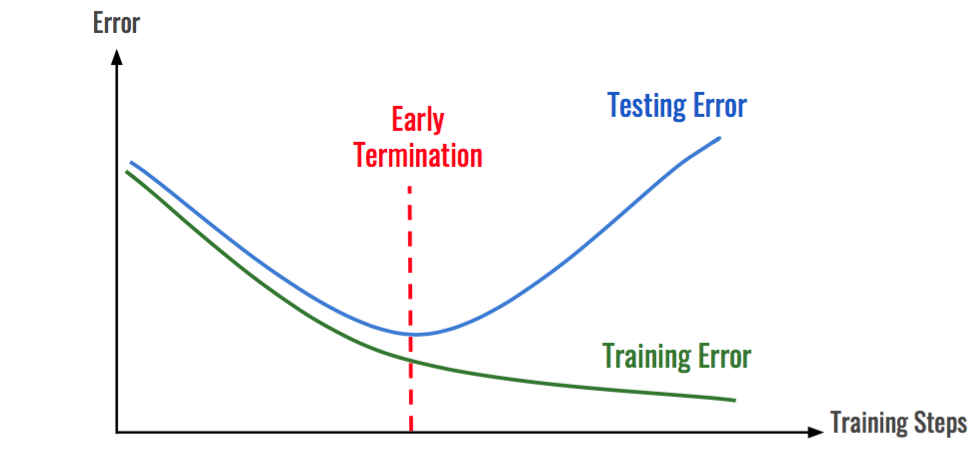
\includegraphics[width=.6\textwidth]{overfitting-nn}
  \caption{Sobreajuste entrenando una red neuronal, tenemos que parar antes de que las curvas diverjan.}
  \label{fig:overfitting-nn}
\end{figure}


\subsection{Teorema de aproximación universal}

Finalmente veamos un resultado matemático que nos permite afirmar con seguridad la fuerte capacidad de las redes neuronales para aprender funciones: el \textbf{teorema de aproximación universal}.

Este teorema tiene dos versiones: el caso de anchura indeterminada, que es la forma clásica, \cite{cybenko1989approximation} y el de profundidad indeterminada \cite{lu2017expressive}.

El caso de anchura arbitraria (\autoref{th:aproxuni-anchura}) nos dice que \textbf{cualquier función continua} en un subconjunto compacto de $R^k$ se puede aproximar con tanta precisión como se quiera con una red neuronal \emph{feed-forward} con una capa oculta y función de activación sigmoide aunque de anchura libre.

\begin{teorema}[Teorema de aproximación universal (anchura indeterminada)]
  Sea $\sigma : \R \to \R$ una función no constante, acotada y continua a la que llamamos función de activación, $I_n$ el hipercubo unidad $n-$dimensional $[0, 1]^n$. Dado un $\epsilon > 0$ y cualquier función $f \in C(I_n)$ entonces $\exists N \in \N$ entero, $\exists \alpha_i, \theta_i \in \R$ constantes reales y $\exists \textbf{w}_i \in \R^n$ vectores reales para $i = 1, \ldots, N$ tal que la función definida como:

  $$F(\textbf{x}) = \sum \limits^N_{i = 1} \alpha_i \sigma \left(\textbf{w}^T_i \textbf{x} + \theta_i \right)$$

  es una realización aproximada de la función $f$, es decir:

  $$|F(\textbf{x}) - f(\textbf{x})| < \epsilon, \; \forall \textbf{x} \in I_n.$$

  En otras palabras, las funciones de la forma $F(\textbf{x})$ son densas en $C(I_n)$. Este resultado también se cumple sustituyendo $I_n$ con cualquier subconjunto compacto de $\R^n$.
  \label{th:aproxuni-anchura}
\end{teorema}

Esta es la versión clásica donde en principio la función $\sigma$ debe ser sigmoide, pero en \cite{leshno1993multilayer} se demuestra que el teorema es cierto para cualquier función $\varphi$ no polinómica. El teorema también se puede extender a cualquier red con profundidad fijada, es decir, con un número de capas ocultas fijo, pero con anchura indeterminada.

Para probar este teorema, primero necesitamos definir cuando una función es \textbf{discriminatoria} \autoref{def:discriminatoria} \cite{cybenko1989approximation}.

\begin{definicion}[Función discriminatoria]
  Sea $M(I_n)$ el espacio de las medidas con signo regulares finitas en $I_n$, una función $\sigma: \R \to \R$ es \textbf{discriminatoria} para una medida $\mu \in M(I_n)$ si:
  $$\int_{I_n} \sigma(\textbf{w}^T \textbf{x} + \theta) d\mu(x) = 0, \; \forall \textbf{w} \in \R^n, \, \forall \theta \in \R \implies \mu = 0.$$
  \label{def:discriminatoria}
\end{definicion}

Ahora probamos el Teorema 1 de \cite{cybenko1989approximation} que es igual que \autoref{th:aproxuni-anchura} pero considerando que $\sigma$ es una función discriminatoria continua.

\begin{teorema}
  Sea $\sigma : \R \to \R$ una función discriminatoria no constante. Dado cualquier $\epsilon > 0$, $f \in C(I_n)$ entonces $\exists N \in \N$ entero, $\exists \alpha_i, \theta_i \in \R$ constantes reales y $\exists \textbf{w}_i \in \R^n$ vectores reales para $i = 1, \ldots, N$ tal que la función definida como:

  $$F(\textbf{x}) = \sum \limits^N_{i = 1} \alpha_i \sigma \left(\textbf{w}^T_i \textbf{x} + \theta_i \right)$$

  es una realización aproximada de la función $f$, es decir:

  $$|F(\textbf{x}) - f(\textbf{x})| < \epsilon, \; \forall \textbf{x} \in I_n.$$

  En otras palabras, las funciones de la forma $F(\textbf{x})$ son densas en $C(I_n)$.
  \label{th:uni1}
\end{teorema}

\begin{proof}
  Sea $S \subset C(I_n)$ el conjunto de funciones de la forma de $F(\textbf{x})$, es trivial que $S$ es un subespacio lineal de $C(I_n)$. Querremos demostrar que la clausura de $S$ es $C(I_n)$.

  Probemos esto por contradicción: supongamos que $R := \overline{S} \neq C(I_n)$ entonces R es un subespacio cerrado propio de $C(I_n)$. Por consecuencia del Teorema de Hahn-Banach (Proposición 3.5 \cite{rudin1973functional}), existe un funcional lineal acotado $L$ en $C(I_n)$ tal que $L \neq 0$ pero $L(R) = L(S) = 0$.

  Por el Teorema de Representación de Riesz \cite{rudin2006real}, este funcional lineal acotado es de la forma

  $$L(h) = \int_{I_n} h(\textbf{x}) d\mu(\textbf{x}), \; \forall h \in C(I_n), \, \mu \in M(I_n).$$

  En particular, como $\sigma(\textbf{w}^T \textbf{x} + \theta)$ está en $R$, $\forall \textbf{w} \in \R^n$, $\forall \theta \in \R$ se debe cumplir que

  $$\int_{I_n} \sigma(\textbf{w}^T \textbf{x} + \theta) d\mu(\textbf{x}) = 0, \; \forall \textbf{w} \in \R^n, \, \forall \theta \in \R.$$

  Sin embargo $\sigma$ era discriminatoria, así que tendríamos que $\mu = 0$  y por tanto $L = 0$ llegando a contradicción. Por tanto, el espacio $S$ debe ser denso en $C(I_n)$.
\end{proof}

Finalmente veamos el Lema 1 de \cite{cybenko1989approximation} que nos dice que las funciones sigmoides continuas son discriminatorias.

\begin{lema}
  Cualquier función sigmoide acotada y medible $\sigma$ es discriminatoria. En particular, cualquier función sigmoide es discriminatoria.
  \label{lema:uni1}
\end{lema}

La demostración de \autoref{th:aproxuni-anchura} queda así demostrada uniendo \autoref{th:uni1} y \autoref{lema:uni1}.

En la otra versión del teorema, de profundidad indeterminada (\autoref{th:aproxuni-prof}), prueba que para toda función Lebesgue-integrable en el espacio de entrada $n$-dimensional respecto la distancia $L^1$ puede ser aproximada por una red neuronal de dimensiones de capa fija $n + 4$ (anchura fija) y función de activación ReLU pero con número de capas ocultas libre.

\begin{teorema}[Teorema de aproximación universal (profundidad indeterminada)]
  Para cualquier función Lebesgue-integrable $f: \R^n \to R$ y cualquier $\epsilon > 0$ existe una red neuronal hacia adelante con función de activación ReLU y anchura $d_m \leq n + 4$ tal que la función $F$ que representa satisface que

  $$\int_{\R^n} |f(\textbf{x}) - F(\textbf{x})| d\textbf{x} < \epsilon.$$
  \label{th:aproxuni-prof}
\end{teorema}

Finalmente cabe añadir que en ambos casos solo se prueba la existencia, no se da una manera para poder construir los pesos ni del tamaño, por lo que el teorema solo nos indica la potencia del espacio de funciones del modelo de las redes neuronales.

\section{Clasificación}

Veamos cómo podemos clasificar las redes neuronales en función del tipo de problema que resuelven o de la arquitectura principal que tienen integrada.

\subsection{Aprendizaje}

Por ser el aprendizaje profundo una subárea del aprendizaje automático, cualquier modelo de red neuronal se puede clasificar atendiendo al tipo de problema que resuelve, donde existen tres ramas principales:

\begin{itemize}
  \item Aprendizaje \textbf{supervisado}: cuando el problema que queremos resolver tiene asociado a los datos unas \textbf{etiquetas}. Se pretende aprender la $f$ desconocida que asigna los datos con las etiquetas mediante la minimización de alguna función de error. Los problemas que ya hemos visto de clasificación y regresión son típicos de aprendizaje supervisado.
  \item Aprendizaje \textbf{no supervisado}: cuando no hay etiquetas, solo nos dan los datos. En este tipo de problemas generalmente se busca patrones y relaciones en los datos, por ejemplo el \textbf{agrupamiento} o \emph{clustering} es un problema típico de aprendizaje no supervisado ya que intenta agrupar los datos en distintos tipos.
  \item Aprendizaje \textbf{por refuerzo}: distinto de los dos anteriores, en estos problemas se intenta enseñar a un modelo como realizar una tarea recompensando o penalizando las acciones que realiza. Crear IAs capaces de jugar al ajedrez, Go o incluso videojuegos entraría dentro de esta categoría.
\end{itemize}

\subsection{Arquitectura}

Veamos aquí distintas arquitecturas con capas más complejas y variadas que han ido surgiendo para intentar abordar problemas de distintos dominios con otros enfoques muy ingeniosos. Obviamos las redes neuronales clásicas que ya hemos explicado y que en cierto sentido podrían considerarse como la red más básica.

\subsection{Redes Neuronales Convolucionales}

Las \textbf{Redes Neuronales Convolucionales} (\emph{Convolutional Neural Networks}, CNN) \cite{lecun1995convolutional} es un tipo de arquitectura orientada al \textbf{tratamiento de imágenes} por lo que se suele usar bastante en problemas cuyos datos sean imágenes de cualquier tipo, en particular prolifera su uso en problemas supervisados de clasificación de imágenes.

Esta arquitectura se basa fundamentalmente en el uso de las \textbf{convoluciones discretas} \eqref{def:convolucion} con las imágenes y un \textbf{tensor} (que puede ser 2D o 3D) denominado \textbf{núcleo} (\emph{kernel}).

\begin{definicion}[Convolución $N$-D discreta]
  Sean dos funciones discretas $f, g : \Z^N \to \R$ definimos la convolución $N$-D discreta de $f$ con $g$ en el punto $\textbf{n} = (n_1, \ldots, n_N)$ como

  $$(f * g)(\textbf{n}) = (f * g)(n_1, \ldots, n_N) = \sum \limits^{+\infty}_{m_1 = -\infty} \ldots \sum^{+\infty}_{m_N = -\infty} f(m_1, \ldots, m_N)g(n_1 - m_1, \ldots, n_M - m_N)$$
  \label{def:convolucion}
\end{definicion}

Esta idea surge de la aplicación de filtros a las imágenes, que se consiguen aplicando estos núcleos convolucionados con la imagen. Los pesos tradicionales que estábamos aprendiendo en las redes se convierten en los valores del núcleo, y lo que se intenta es que la red clasifique imágenes (por ejemplo saber que es un gato o no) \textbf{extrayendo características} que se obtienen al aplicar estos filtros.

Un ejemplo de convolución 2D lo tenemos en \autoref{fig:convolucion-2d} (\cite{pelatrion2020conv}), donde observamos como la convolución realmente es pasar, una matriz en este caso, por la imagen multiplicando coordenada a coordenada y sumando todo el resultado. Esto es extensible fácilmente al caso 3D \autoref{fig:convolucion-3d} (\cite{bansal2018conv}) que es el más usado debido a que las imágenes vienen en 3 canales (RGB) y por tanto pasan de ser matrices (2D) a tensores 3D.

\begin{figure}[htpb]
  \centering
  %\hspace*{-2.5cm}
  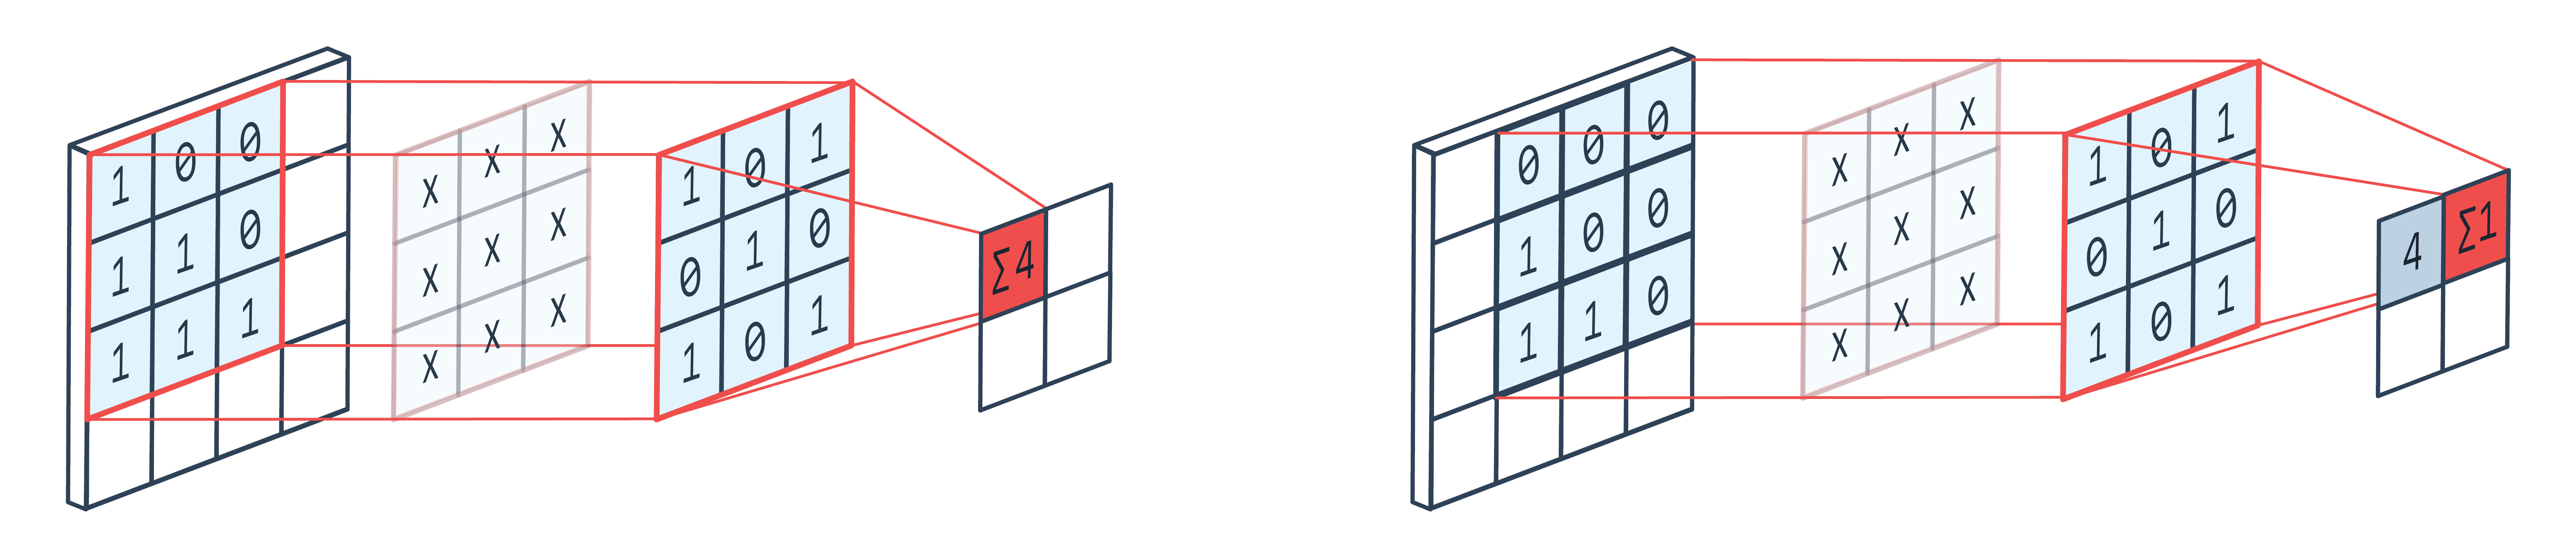
\includegraphics[width=.9\textwidth]{convolucion-2d}
  \caption{Ejemplo de aplicación de convolución 2D.}
  \label{fig:convolucion-2d}
\end{figure}

\begin{figure}[htpb]
  \centering
  %\hspace*{-2.5cm}
  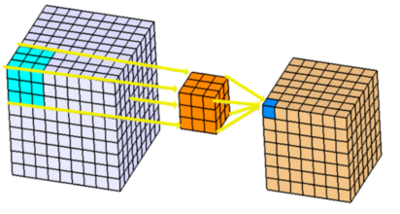
\includegraphics[width=.4\textwidth]{convolucion-3d}
  \caption{Ejemplo de aplicación de convolución 3D.}
  \label{fig:convolucion-3d}
\end{figure}

Notamos que si las imágenes son muy grandes al aplicar diversas capas de filtros el número de pesos puede elevarse bastante y hacerse computacionalmente inviable, por lo que se suele aplicar una técnica de discretización/reducción de dimensión llamada \emph{max-pooling} o \emph{average-pooling }\cite{graham2014fractional}. Esta técnica es igual que aplicar un filtro con $1$ solo que en vez de hacer la suma se toma o bien el máximo o la media de los valores, conseguiendo reducir la dimensión de la imagen tomando representantes de cada área a la que se le aplica; un ejemplo de esto está en \autoref{fig:pooling} \cite{yani2019application}.

\begin{figure}[htpb]
  \centering
  %\hspace*{-2.5cm}
  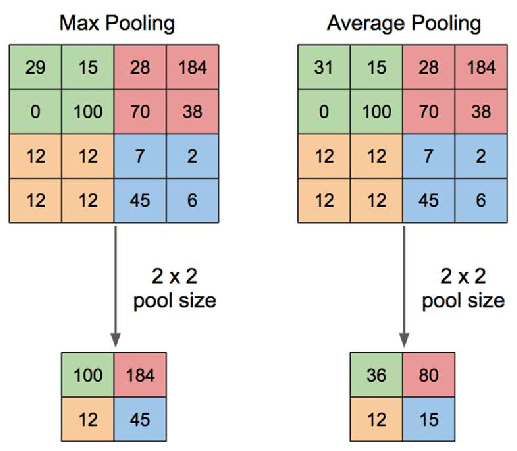
\includegraphics[width=.45\textwidth]{pooling}
  \caption{Ejemplo de \emph{max-pooling} y \emph{average-pooling}.}
  \label{fig:pooling}
\end{figure}

Generalmente la estructura de una CNN tiene dos partes: la primera parte se corresponde al \textbf{extractor de características} que obtiene estas características aplicando filtros mediante el uso de convoluciones con \emph{pooling}, y la segunda es el \textbf{clasificador} que es una red densa (como si fuese una \emph{feed-forward neural network}) que utiliza las características extraídas anteriormente para clasificar las imágenes.

Un ejemplo de esta estructura para clasificar imágenes de dígitos lo tenemos en \autoref{fig:ejemplo-cnn} \cite{saha2018cnn}.

\begin{figure}[htpb]
  \centering
  %\hspace*{-2.5cm}
  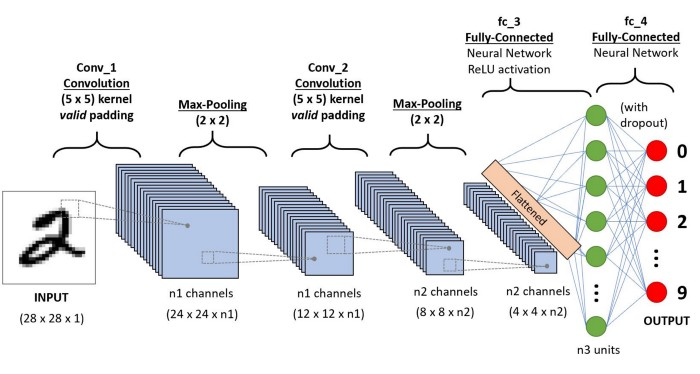
\includegraphics[width=.8\textwidth]{ejemplo-cnn}
  \caption{Ejemplo de estructura de CNN.}
  \label{fig:ejemplo-cnn}
\end{figure}

\subsection{Autocodificador}\label{sec:autoencoder}

Los \textbf{autocodificadores} (\emph{autoencoder, AE}) \cite{mcclelland1986parallel} son redes neuronales modeladas tipicamente para problemas de aprendizaje no supervisado que intentan replicar la entrada en la salida, intentando que en el proceso la red aprenda las características fundamentales de los datos consiguiendo así una \textbf{representación} comprimida de los datos (están codificados).

Veamos la estructura (\autoref{fig:ej-ae}, \cite{sancho2020ae}) que generalmente se divide en dos partes:

\begin{enumerate}
  \item \textbf{Codificador} (\emph{enconder}): la parte de la red que recibe la entrada y va disminuyendo el tamaño de las salidas hasta llegar al vector donde queda codificado la entrada.
  \item \textbf{Descodificador} (\emph{decoder}): la parte de la red que recibe el vector codificador y va aumentado su tamaño hasta llegar a la salida donde reconstruye la entrada original.
\end{enumerate}

\begin{figure}[htpb]
  \centering
  %\hspace*{-2.5cm}
  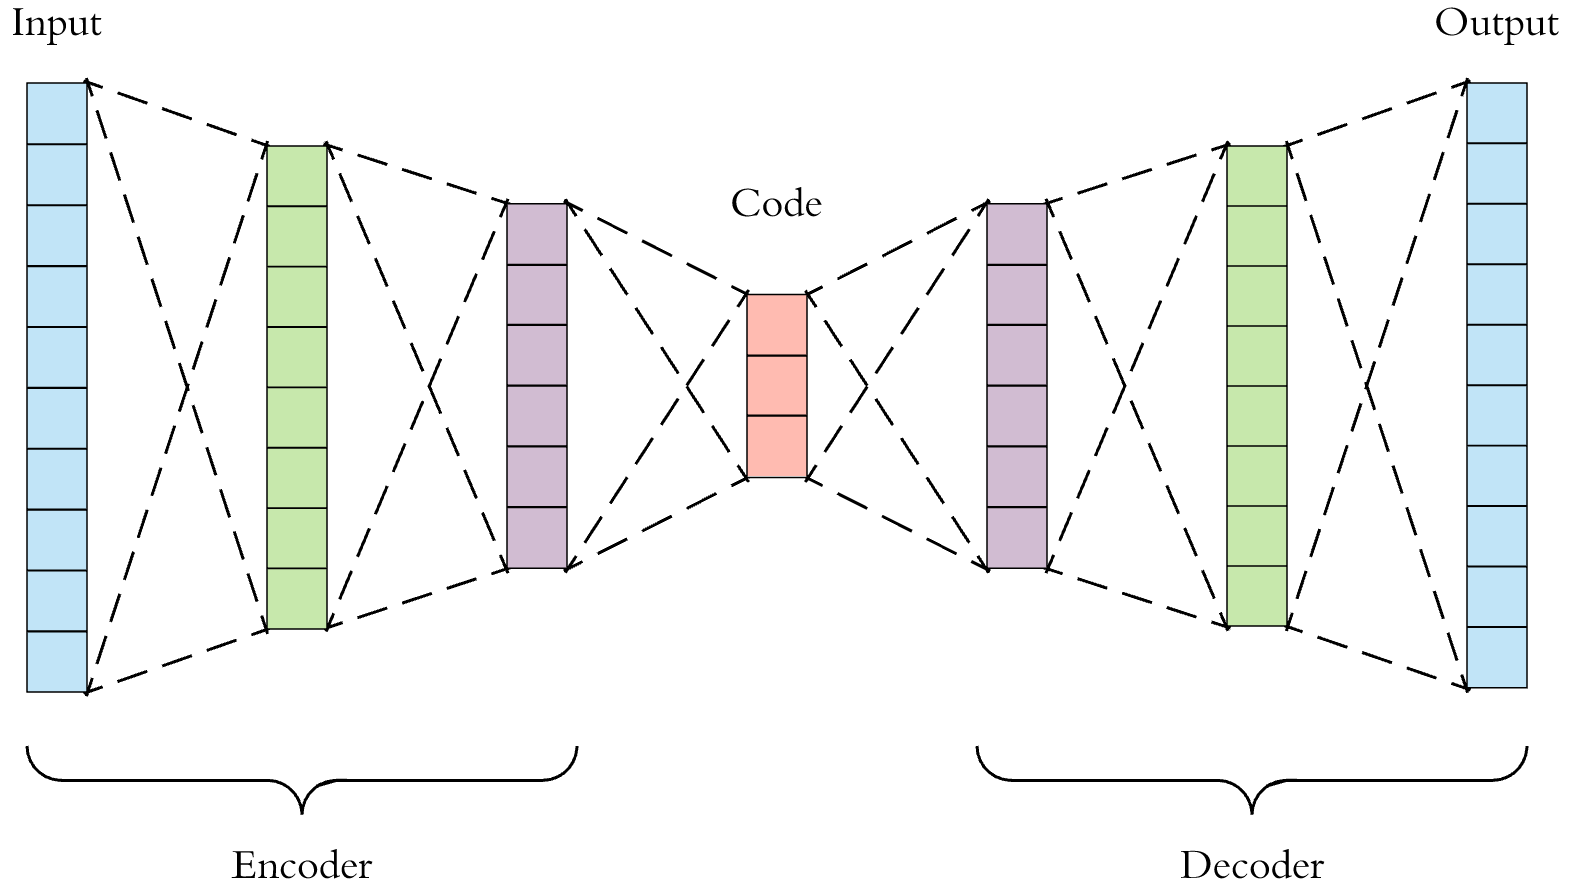
\includegraphics[width=.8\textwidth]{ae}
  \caption{Ejemplo de estructura de un autocodificador}
  \label{fig:ej-ae}
\end{figure}

Este tipo de redes son útiles cuando necesitamos aprender algún patrón o estructura de los datos, o cuando necesitamos comprimir en una dimensión reducida datos muy grandes.

También mencionamos los \textbf{autocodificadores variacionales} (\emph{variational autoencoders}, VAE) que lo que cambian respecto los autocodificadores es el tipo de codificación que se está haciendo, en vez de un vector cualquiera
se busca obtener una representación con \textbf{distribuciones de probabilidad gaussiana}, para ello se toman dos vectores uno de medias $\pmb{\mu} = (\mu_1, \ldots, \mu_n)^T$ y otro de varianzas $\pmb{\sigma}^2 = (\sigma_1^2, \ldots, \sigma_n^2)^T$ de manera que si los juntamos obtenemos un vector de variables aleatorias que siguen distribuciones gausisianas $\mathcal{N}(\pmb{\mu}, diag(\pmb{\sigma}^2))$ de las que podemos obtener una muestra que recontruimos en la salida \autoref{fig:ej-vae} \cite{sancho2020ae}.

\begin{figure}[htpb]
  \centering
  %\hspace*{-2.5cm}
  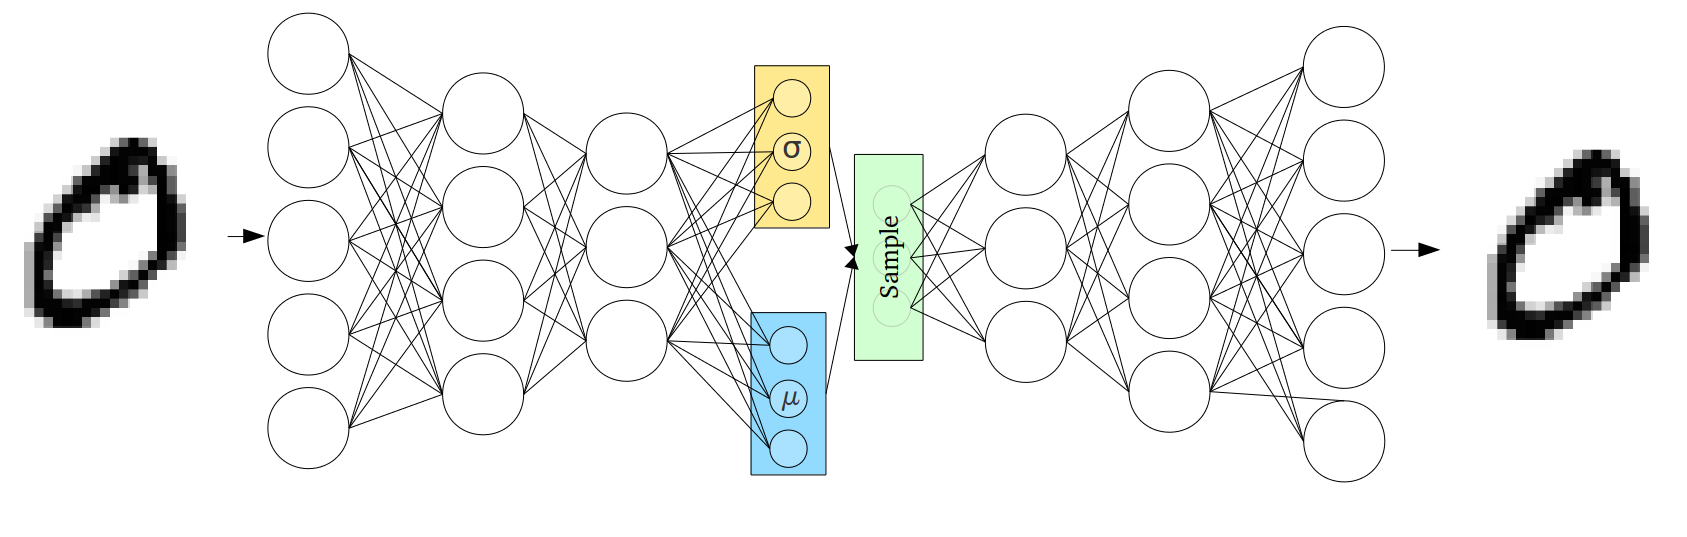
\includegraphics[width=1.\textwidth]{vae}
  \caption{Ejemplo de estructura de un autocodificador variacional}
  \label{fig:ej-vae}
\end{figure}

Para que el entrenamiento se haga correctamente se debe introducir un término nuevo a la función de pérdida que teníamos para la reconstrucción de la entrada: la \textbf{Divergencia de Kullback-Leiber} \cite{kullback1951information} que \emph{a grosso modo} mide la diferencia entre dos distribuciones de probabilidad. Para poder efectuar la diferencia necesitamos saber cual es la distribución latente, pero esta es desconocida así que imponemos la hipótesis de que sea una distribución normal $\mathcal{N}(\textbf{0}, \textbf{1})$ y ya podemos obtener la divergencia como \eqref{eq:divergencia}.

\begin{equation}
  D_{KL}(\mathcal{N}(\pmb{\mu}, diag(\pmb{\sigma}^2)) || \mathcal{N}(\textbf{0}, \textbf{1})) = \dfrac{1}{2} \sum^{n}_{i = 1} \left(\sigma^2_i + \mu^2_i - 1 - \log(\sigma^2_i) \right).
  \label{eq:divergencia}
\end{equation}

Gracias a este diseño, estos modelos son muy útiles para cuando se quieren generar nuevos datos sintéticos que sigan los mismos patrones de los datos donde fueron entrenados, haciendo que parezcan datos auténticos. Por ejemplo podríamos crear un generador de caras en \autoref{fig:caras} \cite{sancho2020ae}.

\begin{figure}[htpb]
  \centering
  %\hspace*{-2.5cm}
  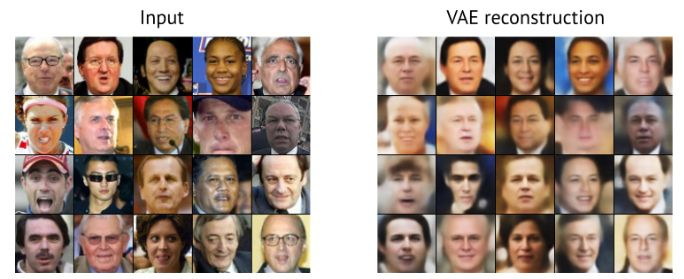
\includegraphics[width=.8\textwidth]{caras}
  \caption{Ejemplo de generador de caras usando un VAE entrenado con caras reales.}
  \label{fig:caras}
\end{figure}

\subsection{Redes Generativas Antagónicas}

Las \textbf{Redes Generativas Antagónicas} (\emph{Generative Adversarial Nets}, GAN) \cite{goodfellow2014generative} es uno de los tipos más novedosos de redes neuronales actualmente cuyo objetivo es crear muestras sintéticas nuevas a partir de una muestra real. Esta arquitectura está compuesta por dos redes distintas: la red \textbf{generadora} (\emph{generator}) y la red \textbf{discriminadora} (\emph{discriminator}). La generadora toma ruido aleatorio como entrada y trata de producir una salida que sea muy parecida a los datos reales, por otro lado la discriminadora toma la entrada del generador y una muestra real del \emph{dataset} y su objetivo es acertar cual es la verdadera (\autoref{fig:gan}, \cite{thalles2018gan}).

\begin{figure}[htpb]
  \centering
  %\hspace*{-2.5cm}
  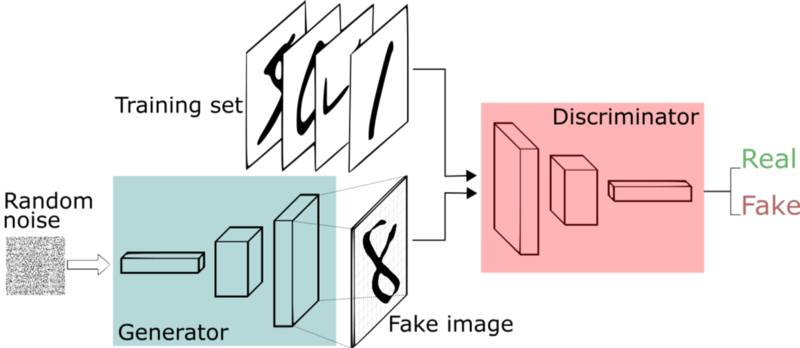
\includegraphics[width=.8\textwidth]{gan}
  \caption{Estructura de una red GAN con dígitos.}
  \label{fig:gan}
\end{figure}

Podemos entender este tipo de red parecido a un juego de suma cero ya que la función de pérdida que intenta minimizar uno es la contraria al otro, por lo que se tiene una especie de \emph{lucha} en el entrenamiento. El generador empieza mejorando los datos fabricados lo que provoca que el discriminador le cueste más diferenciar y se entrene para mejorar su capacidad de discriminación que hace que el generador tenga que hacer mejores fabricaciones; y así cíclicamente, dándonos al final de entrenamiento un generador que devuelve muestras casi imposibles de diferenciar de una real.

Como ya ocurría con los VAE estos modelos son muy útiles para crear datos nuevos que sean prácticamente reales o también para la creación de videos y fotos falsas, modificando las caras de las personas por otras (las famosas \emph{Deepfake} \cite{nguyen2020deepfake}).

\subsection{Redes Neuronales Recurrentes}

Finalmente vemos el tipo de arquitectura en el que nos centraremos, las \textbf{Redes Neuronales Recurrentes} (\emph{Recurrent Neural Networks}, RNN) \cite{elman1990finding} tratan de aprovechar la dependencia temporal que presentan ciertos tipos de datos (frases, música, series temporales...) mediante un flujo de información de entradas anteriores hacia las posteriores (\autoref{fig:rnn-rolled} \cite{christopher2015lstm}).

\begin{figure}[htpb]
  \centering
  %\hspace*{-2.5cm}
  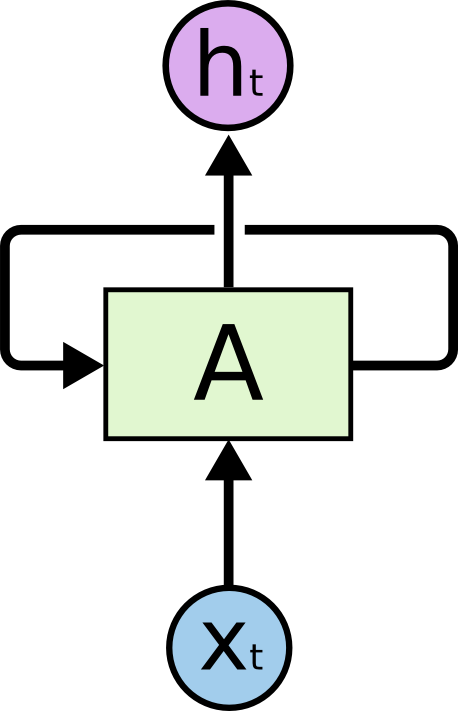
\includegraphics[width=.15\textwidth]{rnn-rolled}
  \caption{Estructura de una RNN.}
  \label{fig:rnn-rolled}
\end{figure}

Esta estructura nos viene a decir que para una cierta entrada $x_t$ el modelo $A$ nos proporciona una salida $h_t$ pero además se pasa a si mismo, retroalimentándose, una información obtenida en función de $x_t$ que se tendrá en cuenta para entradas posteriores ($x_{t + 1}$, $x_{t + 2}$...). Aunque en principio pueda parecer una estructura complicada se puede \emph{desenrollar} en función del tiempo, quedándonos una estructura muy simple (\autoref{fig:rnn-unrolled}, \cite{christopher2015lstm}).

\begin{figure}[htpb]
  \centering
  %\hspace*{-2.5cm}
  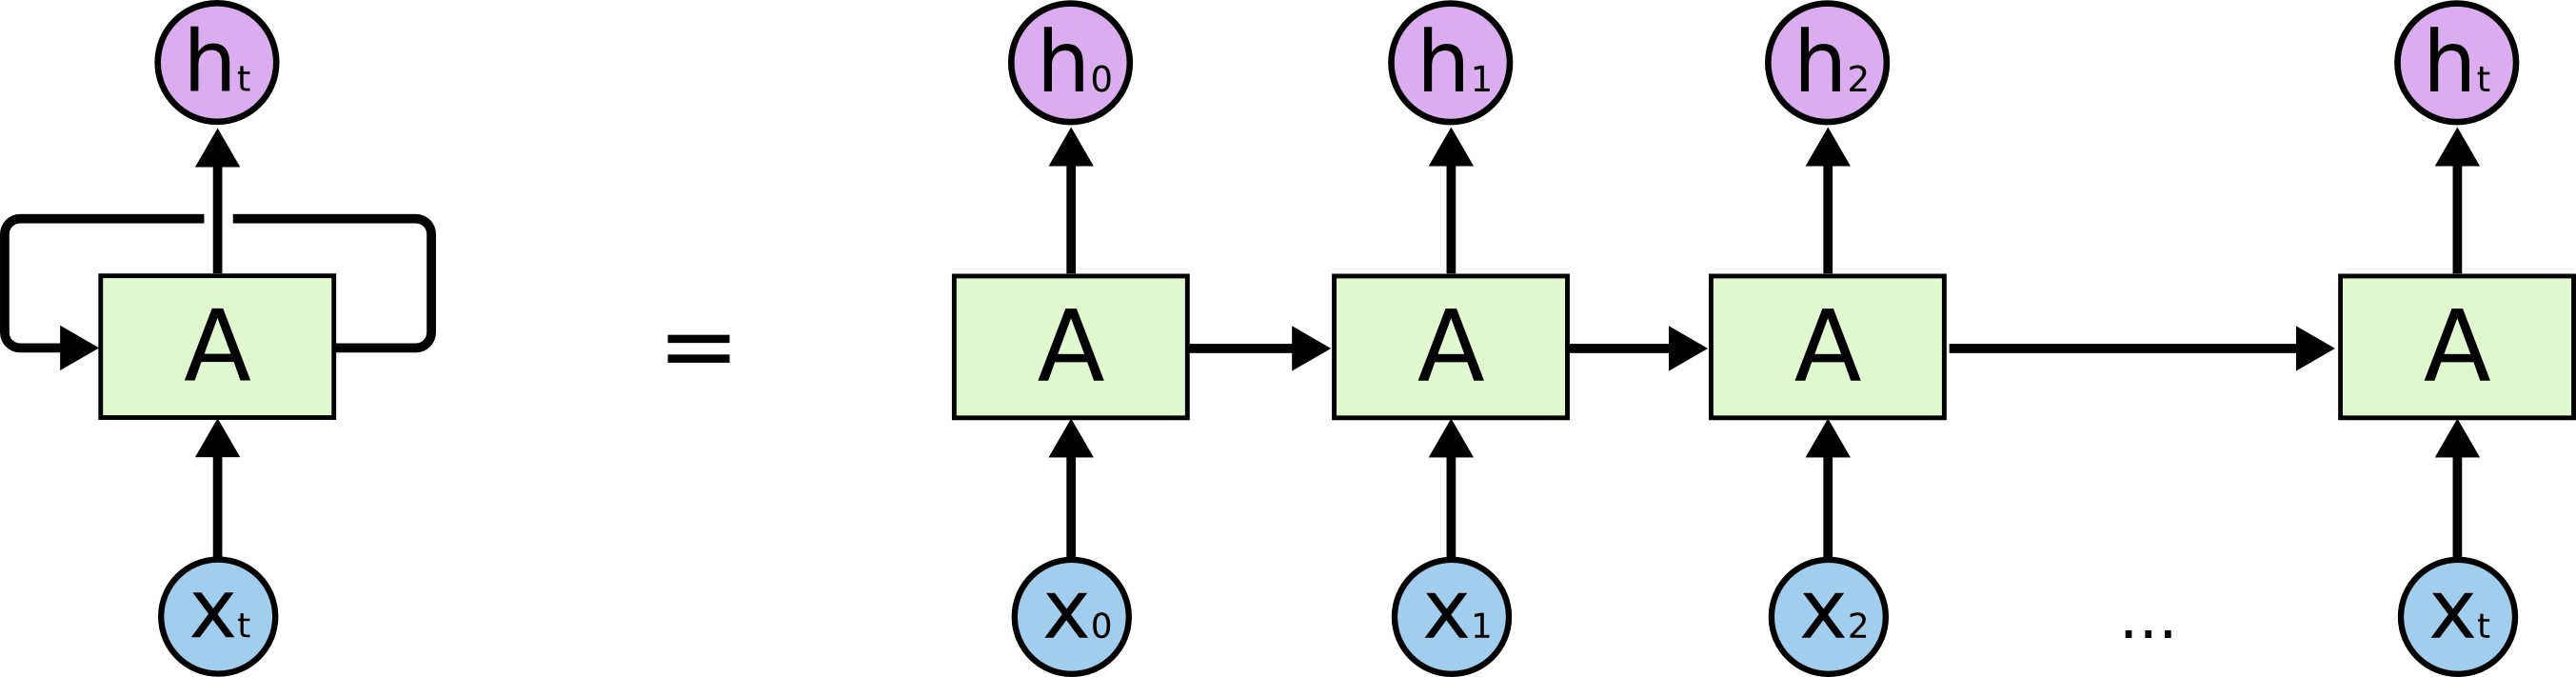
\includegraphics[width=.8\textwidth]{rnn-unrolled}
  \caption{Estructura de una RNN desenrollada.}
  \label{fig:rnn-unrolled}
\end{figure}

Queda claro así cómo según bajo ciertas entradas anteriores, que es lo que proporciona el \textbf{contexto}, la salida de una entrada posterior puede variar enormemente. Así, en las RNN se diseña una neurona especial para enviar la información de manera relativamente sencilla: se une la entrada $x_t$ con la salida de la entrada anterior $h_{t-1}$, que llamaremos \textbf{estado oculto}, a una neurona normal como las conocemos (pesos más una función de activación). La fórmula de cada neurona quedará terminada por los pesos $W$ y la fórmula \eqref{eq:rnn} (\autoref{fig:rnn-cells}, \cite{christopher2015lstm}) tomando como función de activación $\tanh$.

\begin{equation}
  h_t = \tanh \left(W^T \begin{bmatrix} h_{t-1} & x_t & 1 \end{bmatrix}^T\right).
  \label{eq:rnn}
\end{equation}

\begin{figure}[htpb]
  \centering
  %\hspace*{-2.5cm}
  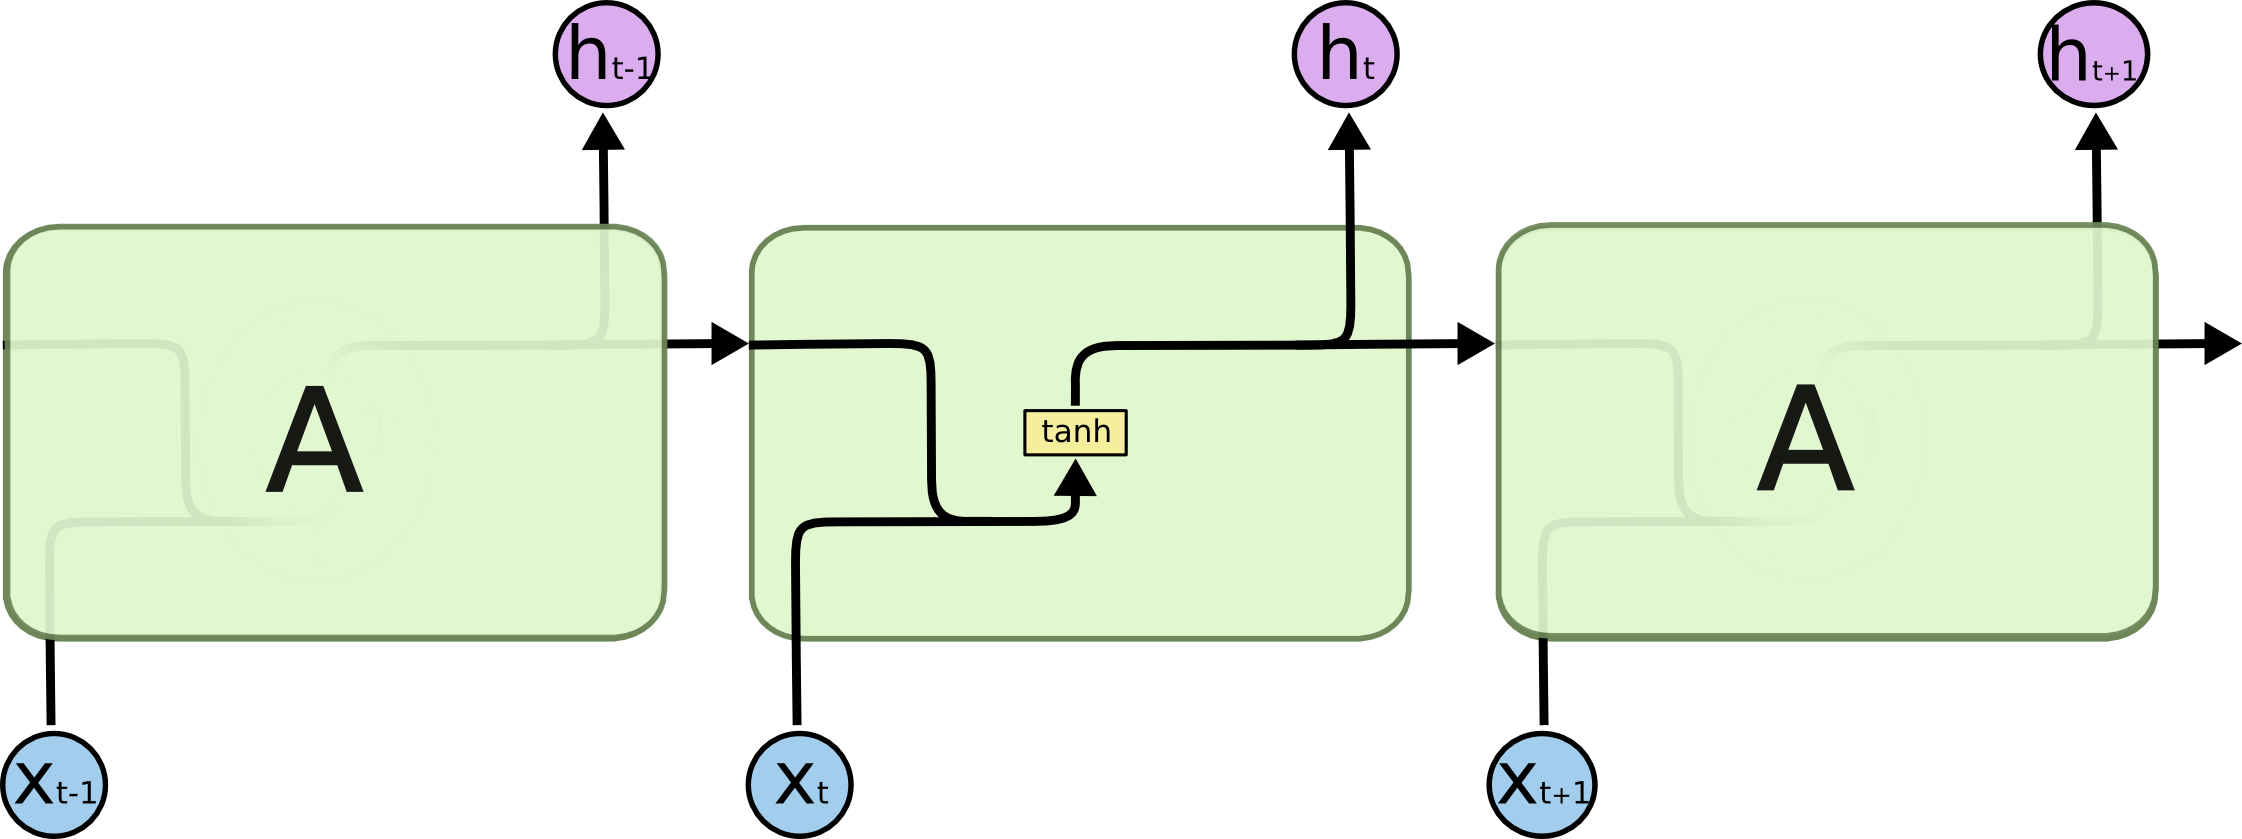
\includegraphics[width=.9\textwidth]{rnn-cells}
  \caption{Estructura de una neurona en una RNN.}
  \label{fig:rnn-cells}
\end{figure}

Sin embargo hay un gran problema: cierta información útil para una entrada \textbf{muy posterior} en el tiempo probablemente no llegue debido a que hay un salto temporal muy grande entre las entradas (\autoref{fig:rnn-longterm}, \cite{christopher2015lstm}), es decir, el modelo no capta bien las \textbf{dependencias temporales a largo plazo} (\emph{long-term dependecies}) \cite{bengio1994learning}.

\begin{figure}[htpb]
  \centering
  %\hspace*{-2.5cm}
  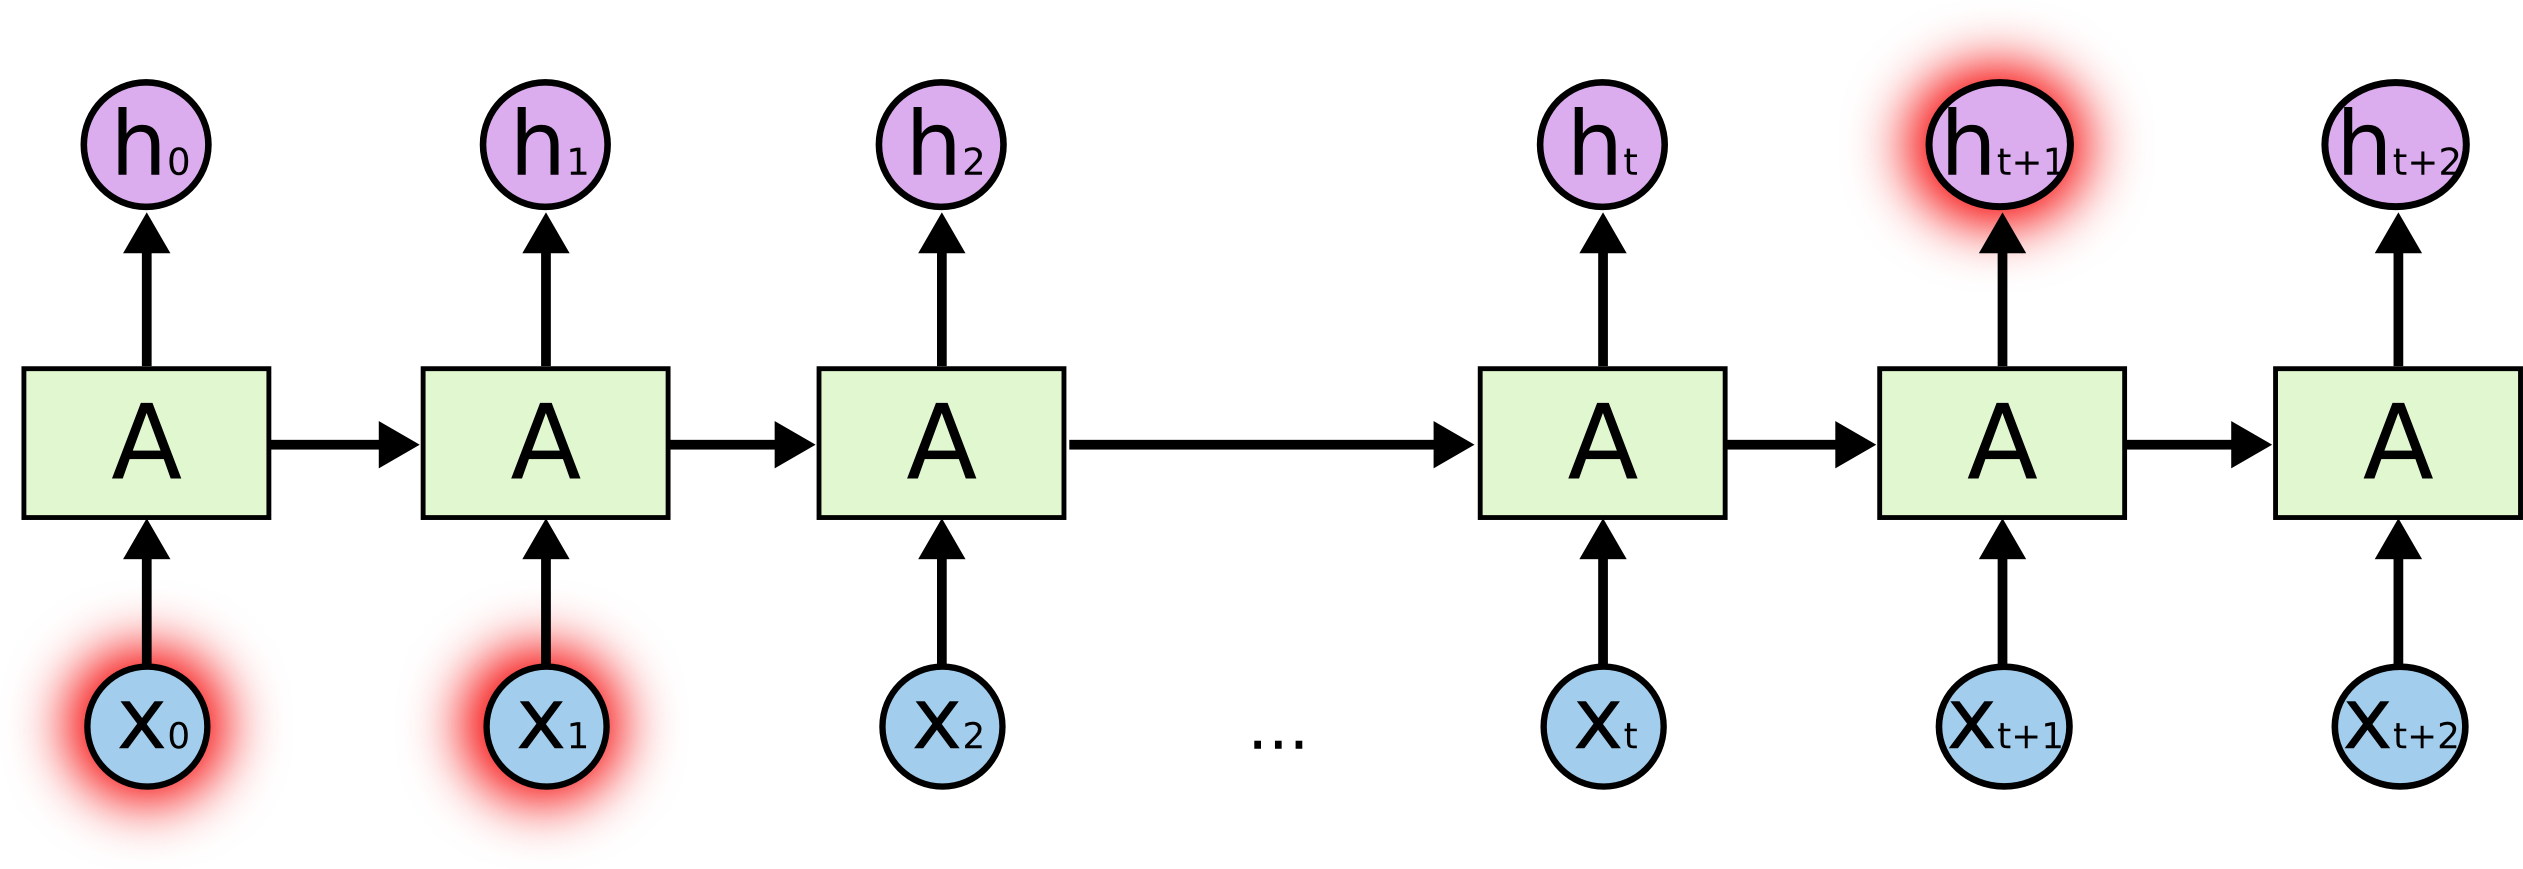
\includegraphics[width=.9\textwidth]{rnn-longterm}
  \caption{La información de $x_1$ y $x_2$ no llega para $h_{t+1}$.}
  \label{fig:rnn-longterm}
\end{figure}

Este obstáculo es consecuencia directa del \textbf{problema del desvanecimiento del gradiente} (\emph{vanishing gradient problem}) que ocurre al entrenar redes neuronales muy profundas, ya que, recordando que para obtener el gradiente íbamos propagando el error desde la última capa hasta la primera capa, el gradiente va disminuyendo poco a poco y si la red es muy extensa entonces va disminuyendo a cero provocando que las capas dejen de actualizarse. Lo que viene a decirnos resumidamente es que la información se pierde rápidamente en el tiempo, por lo que no podemos dar información de entradas muy separadas. También es posible que pase el caso contrario, que el gradiente \textbf{explote} (\emph{explodes}) (aumente hasta valores que sobrepasan el límite de representación de la máquina); en cualquier caso las RNN suelen ser modelos inestables debido a esto \cite{Goodfellow-et-al-2016}.

Para resolver este problema surgen las redes \emph{Long Short Term Memory} (LSTM) \cite{hochreiter1997long}, que consiguen aprender la información tanto a corto como a largo plazo. Estas redes serán las que dedicaremos más atención, y sobre las que nos basaremos para construir nuestros modelos de aprendizaje profundo en el desarrollo del trabajo.

\section{LSTM}

\subsection{Estructura general}

La idea que añade una neurona LSTM para solucionar las dependencias temporales a largo plazo es permitir el paso de la información, recordando u olvidándola, mediante \textbf{puertas} (\emph{gates}) y añadiendo otro flujo de información además del estado oculto $h_t$: el estado celular $C_t$. Este estado intenta emular una especie de \emph{memoria} que irá llevando información relevante desde el principio de la secuencia de entradas hasta mucho más adelante, evitando la pérdida a largo plazo de las RNN.

Primero veamos como está constituida una puerta (\autoref{fig:gate}, \cite{christopher2015lstm}): una neurona normal que recibe una entrada y con función de activación \textbf{sigmoide}, cuya salida realiza una operación de multiplicación coordenada a coordenada con la información que se está regulando. Como la función sigmoide devuelve valores entre $[0, 1]$, al multiplicarlos por la información nos permite, o bien olvidar cuando los valores sean cercanos a 0 ó recordarlos si son cercanos a 1.

\begin{figure}[htpb]
  \centering
  %\hspace*{-2.5cm}
  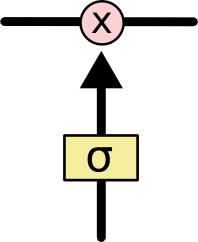
\includegraphics[width=.2\textwidth]{gate}
  \caption{Ejemplo de puerta.}
  \label{fig:gate}
\end{figure}

Fijémonos ahora en la estructura general de una neurona o célula LSTM (\autoref{fig:lstm-cells}, \cite{christopher2015lstm}) y vayamos paso por paso para entender todas los operaciones que tienen lugar. Apreciamos cómo el estado celular viene dado por el flujo superior de la célula, mientras que el estado oculto entra y sale por el inferior y consideramos además que $\sigma \equiv sigmoide$.

\begin{figure}[htpb]
  \centering
  %\hspace*{-2.5cm}
  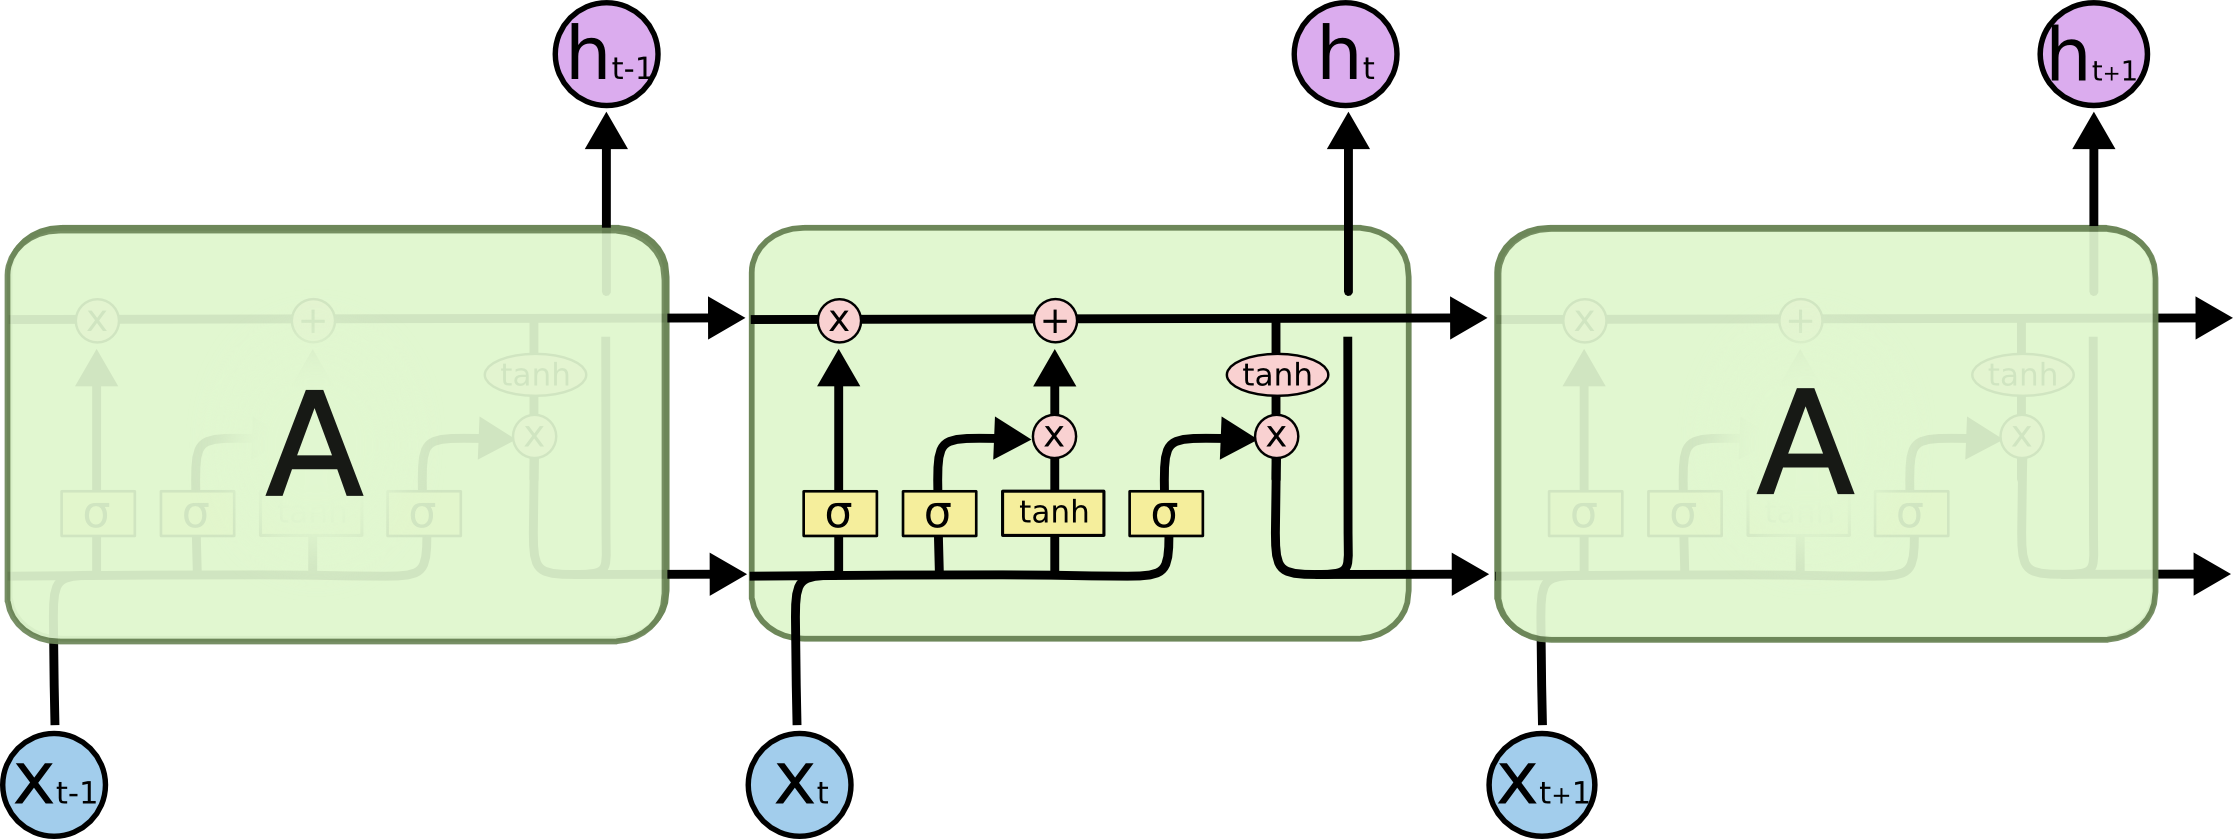
\includegraphics[width=1.\textwidth]{lstm-cells}
  \caption{Esquema de célula LSTM.}
  \label{fig:lstm-cells}
\end{figure}

Primero nos encontramos con la \textbf{puerta del olvido} (\emph{forget gate}), la puerta que se encarga de decidir si la información del estado celular anterior $c_{t-1}$ debería olvidarse o no en base a el estado oculto anterior $h_{t-1}$ y la entrada actual $x_t$; de esta manera controlamos qué información de las variables anteriores recordamos. El valor de la puerta $f_t$ queda determinado por los pesos $W_f$ y en base a \eqref{eq:forget} (\autoref{fig:forget} \cite{christopher2015lstm}).

\begin{equation}
  f_t = \sigma\left(W_f^T \begin{bmatrix} h_{t-1} & x_t & 1 \end{bmatrix}^T \right).
  \label{eq:forget}
\end{equation}

\begin{figure}[htpb]
  \centering
  %\hspace*{-2.5cm}
  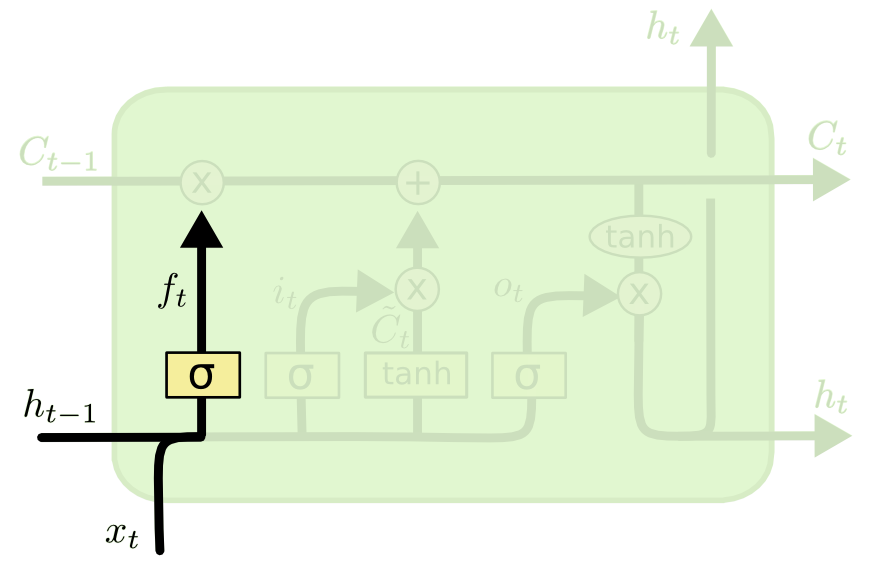
\includegraphics[width=.5\textwidth]{forget}
  \caption{Puerta del olvido $f_t$.}
  \label{fig:forget}
\end{figure}

A continuación tenemos la \textbf{puerta de entrada} (\emph{input gate}) que es la que determina si la nueva información en base a la entrada actual $x_t$ y el estado oculto anterior $h_{t-1}$, se debe incluir o no en el estado celular; indicándonos si esta entrada es relevante o no. Tenemos por un lado el valor de la puerta $i_t$ y el valor de la neurona que tiene la información $\widetilde{C}_t$ donde ambas quedan determinadas por sus pesos $W_i$, $W_{\widetilde{C}}$ y con las fórmulas \eqref{eq:input1}, \eqref{eq:input2} respectivamente (\autoref{fig:input} \cite{christopher2015lstm}).

\begin{equation}
  i_t = \sigma\left(W_i^T \begin{bmatrix} h_{t-1} & x_t & 1 \end{bmatrix}^T\right),
  \label{eq:input1}
\end{equation}

\begin{equation}
  \widetilde{C}_t = \tanh\left(W_{\widetilde{C}}^T \begin{bmatrix} h_{t-1} & x_t & 1 \end{bmatrix}^T\right).
  \label{eq:input2}
\end{equation}

\begin{figure}[htpb]
  \centering
  %\hspace*{-2.5cm}
  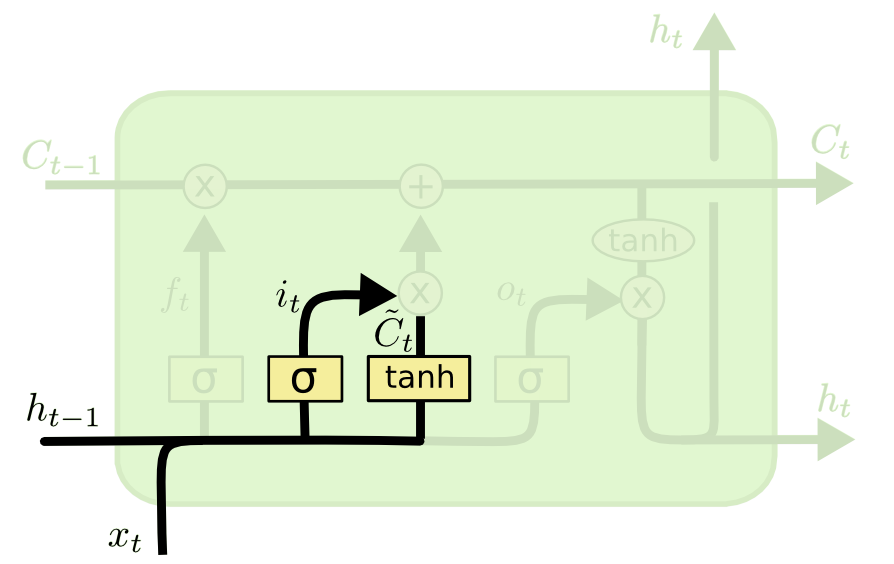
\includegraphics[width=.5\textwidth]{input}
  \caption{Puerta de entrada $i_t$ e información de la neurona $\widetilde{C}_t$.}
  \label{fig:input}
\end{figure}

Llegamos al \textbf{estado celular} que es el valor que lleva la información importante a lo largo de la secuencia y que queda determinada por su entrada anterior $C_{t-1}$ junto a la puerta del olvido $f_t$ y la información actual $\widetilde{C}_t$ junto a la puerta de entrada $i_t$. Su valor $C_t$ queda determinada por los valores anteriores en base a la fórmula \eqref{eq:celular} (\autoref{fig:celular} \cite{christopher2015lstm}).

\begin{equation}
  C_t = f_t C_{t-1} + i_t \widetilde{C}_t.
  \label{eq:celular}
\end{equation}

\begin{figure}[htpb]
  \centering
  %\hspace*{-2.5cm}
  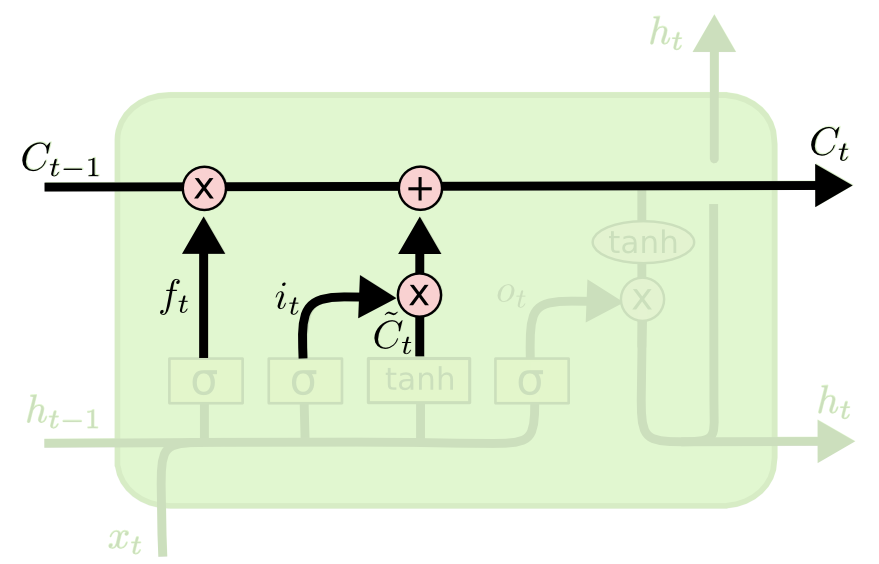
\includegraphics[width=.5\textwidth]{celular}
  \caption{Estado celular $C_t$.}
  \label{fig:celular}
\end{figure}

Finalmente acabamos con la \textbf{puerta de salida} (\emph{output gate}) que regula la información del estado celular $C_t$ que devuelve como salida la célula, es decir, el estado oculto $h_t$. Tenemos el valor de la puerta $o_t$, determinado por la última matriz de pesos $W_o$, y el estado celular $h_t$ calculados con las fórmulas \eqref{eq:output1} \eqref{eq:output2} respectivamente (\autoref{fig:output} \cite{christopher2015lstm}).

\begin{equation}
  o_t = \sigma\left(W_o^T \begin{bmatrix} h_{t-1} & x_t & 1 \end{bmatrix}^T\right),
  \label{eq:output1}
\end{equation}

\begin{equation}
  h_t = o_t \tanh\left(C_t\right).
  \label{eq:output2}
\end{equation}

\begin{figure}[htpb]
  \centering
  %\hspace*{-2.5cm}
  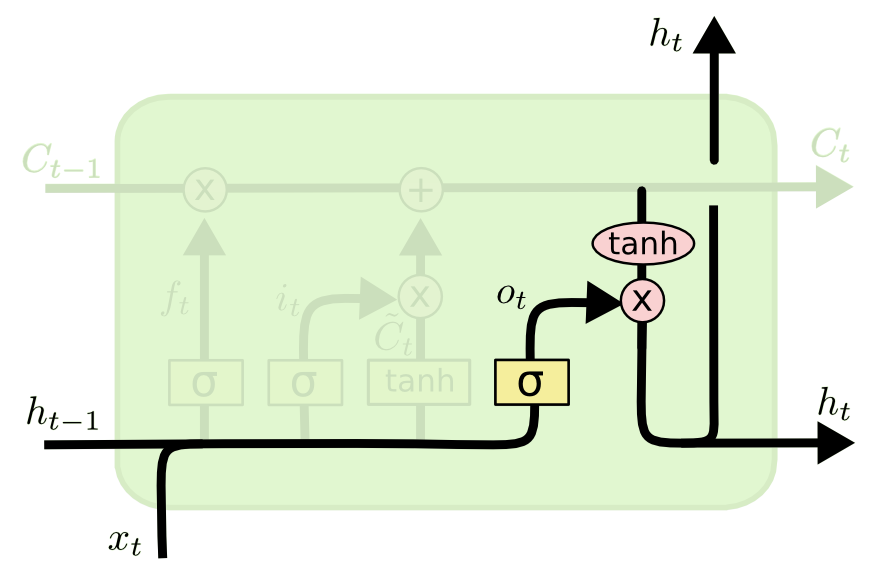
\includegraphics[width=.5\textwidth]{output}
  \caption{Puerta de salida $o_t$.}
  \label{fig:output}
\end{figure}

Observamos que cada célula LSTM tiene 4 neuronas normales con sus pesos respectivos que aprender, siendo de estas 3 para puertas (olvido, entrada y salida) y la cuarta para la información de la propia célula. Este tipo de neurona es mucho más compleja y con muchos mas parámetros libres que aprender que la versión que habíamos considerado en las RNN pero permite flujos de información mucho más ricos al permitir olvidar o memorizar a voluntad y por supuesto que se pueda transmitir información importante desde tiempos muy separados.

\subsection{Variantes}

De esta célula se han creado muchas variantes que generalmente suelen ser modificaciones pequeñas que son ciertamente interesantes. Por ejemplo, \cite{gers2000recurrent} añade conexiones del estado celular anterior $C_{t-1}$ hacia las puertas de manera que los valores quedan actualizados así \eqref{eq:variante1} (\autoref{fig:variante1} \cite{christopher2015lstm}).

\begin{gather}
  f_t = \sigma\left(W_f^T \begin{bmatrix} C_{t-1} & h_{t-1} & x_t & 1 \end{bmatrix}^T \right), \\
  i_t = \sigma\left(W_i^T \begin{bmatrix} C_{t-1} & h_{t-1} & x_t & 1 \end{bmatrix}^T\right), \\
  o_t = \sigma\left(W_o^T \begin{bmatrix} C_{t-1} & h_{t-1} & x_t & 1 \end{bmatrix}^T\right).
  \label{eq:variante1}
\end{gather}

\begin{figure}[htpb]
  \centering
  %\hspace*{-2.5cm}
  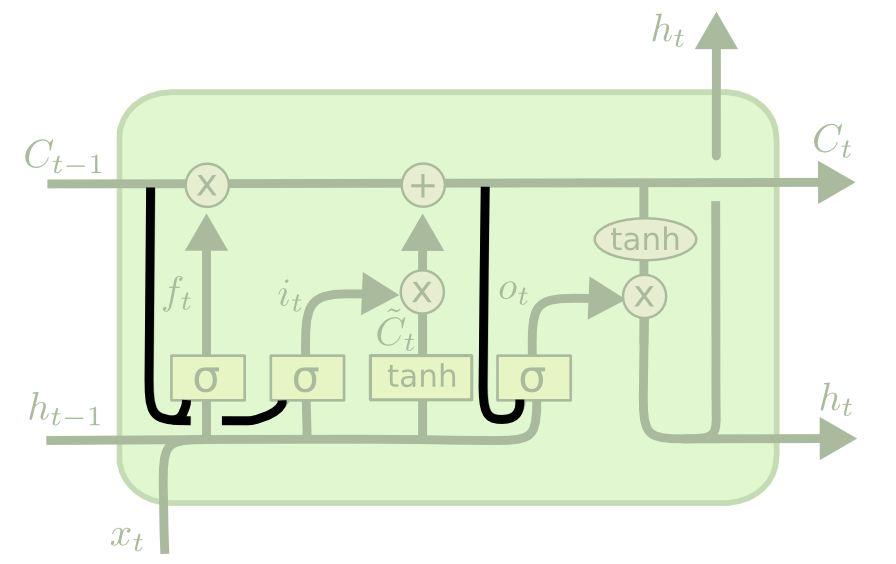
\includegraphics[width=.5\textwidth]{variante1}
  \caption{Variante que introduce cauces de $C_{t-1}$ con las puertas.}
  \label{fig:variante1}
\end{figure}

Otra modificación de \cite{gers2000recurrent} considera unificar las puertas de olvido $f_t$ y entrada $i_t$ de manera que si una puerta considera olvidar la información la otra puerta recuerda; de esta manera solo recordamos algo nuevo si olvidamos lo pasado, y solo recordamos lo pasado si olvidamos lo nuevo. Las fórmulas de $C_t$ y $i_t$ actualizadas se quedan así \eqref{eq:variante2} (\autoref{fig:variante2} \cite{christopher2015lstm}).

\begin{gather}
  i_t = 1 - f_t, \\
  C_t = f_t C_{t-1} + (1 - f_t) \widetilde{C}_t.
  \label{eq:variante2}
\end{gather}

\begin{figure}[htpb]
  \centering
  %\hspace*{-2.5cm}
  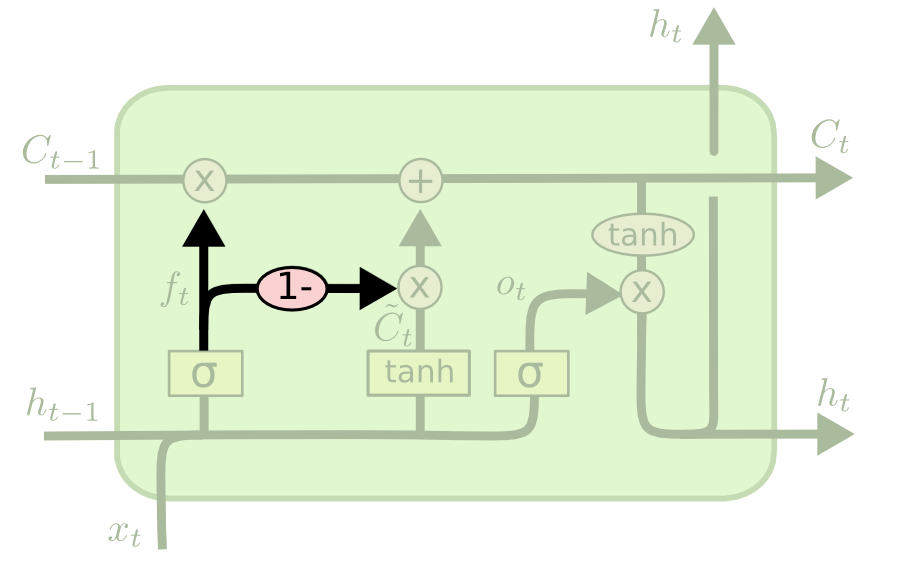
\includegraphics[width=.5\textwidth]{variante2}
  \caption{Variante que sustituye la puerta de entrada por la negación de la del olvido.}
  \label{fig:variante2}
\end{figure}

Finalmente nombramos una de las variantes más conocidas, la \textbf{Unidad Recurrente con Puertas} (\emph{Gated Recurrent Unit}, GRU) \cite{cho2014learning} que intenta simplificar la célula LSTM para reducir los cálculos y conseguir un entrenamiento mucho más rápido mediante la fusión el estado celular con el oculto, así como también las puertas del olvido y de entrada (formando la puerta de actualización $z_t$), quitando la puerta de salida y añadiendo una nueva llamada de reinicio $r_t$. Ahora la célula solo devuelve el estado oculto $h_t$ en función de la siguientes fórmulas \eqref{eq:gru} junto a la nueva estructura (\autoref{fig:gru}, \cite{christopher2015lstm}).

\begin{gather}
  z_t = \sigma\left(W_z^T \begin{bmatrix} h_{t-1} & x_t \end{bmatrix}^T\right), \\
  r_t = \sigma\left(W_r^T \begin{bmatrix} h_{t-1} & x_t \end{bmatrix}^T \right), \\
  \widetilde{h}_t = \tanh\left(W_{\widetilde{h}}^T \begin{bmatrix} r_t h_{t-1} & x_t \end{bmatrix}^T\right), \\
  h_t = (1 - z_t)h_{t-1} + z_t \widetilde{h}_t.
  \label{eq:gru}
\end{gather}

\begin{figure}[htpb]
  \centering
  %\hspace*{-2.5cm}
  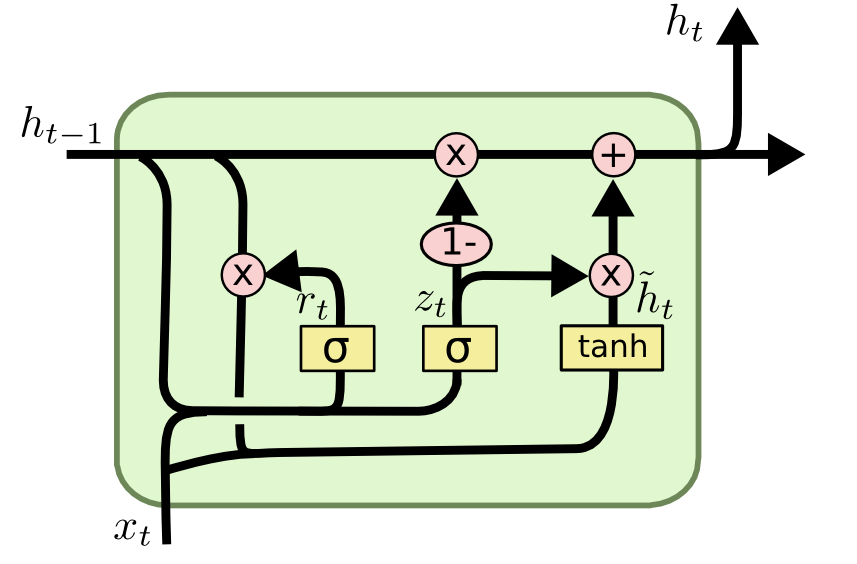
\includegraphics[width=.5\textwidth]{gru}
  \caption{Estructura de la variante GRU.}
  \label{fig:gru}
\end{figure}

Sin embargo, en \cite{greff2016lstm} se hace una comparación de rendimiento entre todas variantes y se observó que no había un modelo que fuese especialmente mejor, todas se comportaban más o menos igual de bien, si bien \cite{gers1999learning} observaron que la versión de LSTM añadiendo un término de error de 1 en la puerta del olvido la hacía la versión más potente de todas las consideradas \cite{Goodfellow-et-al-2016}. Bajo estas razones tomaremos en nuestros modelos las versiones LSTM normales.

\subsection{Recorte}

A pesar de que la arquitectura LSTM evita enormemente el problema del desvanecimiento del gradiente, es posible encontrar en algún caso de entrenamiento que el gradiente explote (la norma del gradiente diverge). Si ocurre esto una técnica muy interesante de utilizar es el método del \textbf{recorte de gradiente} (\emph{clipping gradient}) \cite{pascanu2013difficulty}, que se encarga de ponerle un \emph{tope} a la norma del gradiente cuando supera cierto valor.

Cada vez que se obtiene el gradiente $\textbf{g}$ se aplica la siguiente regla \eqref{eq:clipping} antes de actualizar los pesos, evitando así que la red use valores enormes del gradiente para actualizar los pesos, haciendo que la red se inestabilice y ya no sirva \cite{Goodfellow-et-al-2016}.

\begin{equation}
  \textbf{g}' = \begin{cases} \textbf{g} & \text{si } ||\textbf{g}|| \leq v \\ v\dfrac{\textbf{g}}{||\textbf{g}||} & \text{en caso contrario} \end{cases}.
  \label{eq:clipping}
\end{equation}

\endinput

% !TeX root = ../libro.tex
% !TeX encoding = utf8
%
%*******************************************************
% Series Temporales
%*******************************************************

\chapter{Series Temporales}\label{ch:st}

Presentamos y explicamos la teoría sobre las \textbf{series temporales}, los objetos de estudio que se presentarán en nuestros problemas y que se usarán en los modelos realizados.

Usaremos como base para desarrollar esta parte la literatura para series temporales y procesos estocásticos, concretamente de \cite{cox1977theory}, \cite{chatfield2019analysis}, \cite{brockwell2002introduction}, \cite{hyndman2018forecasting}, \cite{box2011time} y \cite{grandell1998time}.

\section{Definición y características}

Para ver qué es y poder estudiar una serie temporal necesitamos tener una base de la teoría de \textbf{procesos estocásticos}. Esta teoría se encarga de estudiar sistemas que evolucionan en el \textbf{tiempo} en función de \textbf{leyes probabilísticas}.

\subsection{Elementos básicos}

Para explicar estos conceptos vamos a hacer un breve recordatorio de los elementos fundamentales que juegan un papel en la teoría de la probabilidad, que se basa en el estudio de ciertas \textbf{funciones} reales que parten de un espacio donde hay una \textbf{medida de probabilidad}.

La idea del espacio que hemos mencionado es muy simple: queremos asignar a \textbf{subconjuntos} (sucesos) de cierto \textbf{espacio} una cantidad numérica que representa la \textbf{probabilidad} de que ocurran. Por tanto necesitaremos un espacio $\Omega$, una $\sigma$-álgebra $\mathcal{A}$ sobre $\Omega$ (\autoref{def:sigma-algebra}) y una función de probabilidad $P$ en $\Omega$ (\autoref{def:probabilidad}).

\begin{definicion}[$\sigma$-álgebra]
  Sea un conjunto $\Omega$, una $\sigma$-álgebra sobre $\Omega$ es una familia $\mathcal{A}$ de subconjuntos de $\Omega$ que incluye el espacio entero y es cerrada bajo complementos y uniones numerables; es decir, que cumple lo siguiente:
  \begin{enumerate}
    \item $\Omega \in \mathcal{A}$.
    \item $\forall A \in \mathcal{A} \implies \overline{A} \in \mathcal{A}$.
    \item $\forall \{A_n\}_{n \in \N} \subseteq \mathcal{A} \implies \bigcup \limits^\infty_{n = 1} A_n \in \mathcal{A}$
  \end{enumerate}
  \label{def:sigma-algebra}
\end{definicion}

\begin{definicion}[Función de probabilidad]
  Sea un espacio $\Omega$, y $\mathcal{A}$ una $\sigma$-álgebra sobre $\Omega$, una función de probabilidad $P : \mathcal{A} \to R$ es una función que cumple lo siguiente:

  \begin{itemize}
    \item (No negativa): $\forall A \in \mathcal{A}, \, P(A) \geq 0$
    \item (Normalización): $P(\Omega) = 1$
    \item ($\sigma$-aditividad): $\forall \{A\}_{n \in \N} \subseteq \mathcal{A}$ disjuntos 2 a 2 $\implies P \left(\bigcup \limits^\infty_{n = 1} A_n \right) = \sum \limits^\infty_{n = 1} P(A_n)$
  \end{itemize}
  \label{def:probabilidad}
\end{definicion}

Juntando estos tres elementos obtenemos nuestro \textbf{espacio probabilístico} (\autoref{def:espacio-probabilistico}).

\begin{definicion}[Espacio probabilístico]
  Sea $\Omega$ un conjunto, $\mathcal{A}$ una $\sigma$-álgebra sobre $\Omega$ y $P$ una probabilidad en $\Omega$, entonces definimos el espacio de probabilidad como la terna $(\Omega, \mathcal{A}, P)$.
  \label{def:espacio-probabilistico}
\end{definicion}

Como la probabilidad $P$ es realmente una medida normalizada, podemos aplicar aspectos de la teoría de la medida en un espacio probabilístico. En concreto consideraremos funciones medibles, que son aplicaciones medibles (\autoref{def:aplicacion-medible}) donde el espacio de llegada es un espacio \textbf{Borel} ($\sigma$-álgebra formada con las semirrectas cerradas por la derecha $(-\infty, x]$).

\begin{definicion}[Aplicación medible]
  Sean dos espacios medibles $(\Omega_1, \mathcal{A}_1)$, $(\Omega_2, \mathcal{A}_2)$, una aplicación $f : \Omega_1 \to \Omega_2$ se dice medible, si y solamente si:

  $$\forall A \in \mathcal{A}_2, \, f^{-1}(A) = \{\omega \in \Omega_1 : f(\omega) \in A\} \in \mathcal{A}_1$$
  \label{def:aplicacion-medible}
\end{definicion}

Definimos así las funciones que forman la base de esta teoría: las \textbf{variables aleatorias} (\autoref{def:var-aleatoria}). Hemos tomado el espacio Borel usual como $(\R, \mathcal{B})$ aunque si tenemos un subconjunto $E \subseteq \R$ se puede considerar el espacio Borel $(E, \mathcal{B}_E)$ donde $\mathcal{B}_E$ es la $\sigma$-álgebra Borel restringida a $E$.

\begin{definicion}[Variable aleatoria]
  Sea un espacio de probabilidad $(\Omega, \mathcal{A}, P)$, una variable aleatoria es una función medible de un espacio de probabilidad en un espacio Borel $X: (\Omega, \mathcal{A}, P) \to (\R, \mathcal{B})$.
  \label{def:var-aleatoria}
\end{definicion}

Una variable aleatoria $X$ induce una probabilidad en el espacio de llegada Borel que denominamos como \textbf{función de probabilidad} (\autoref{def:distribucion-probabilidad}).

\begin{definicion}[Distribución de probabilidad]
  Sea un espacio probabilístico $(\Omega, \mathcal{A}, P)$ y una variable aleatoria $X: (\Omega, \mathcal{A}, P) \to (\R, \mathcal{B})$, llamamos distribución de probabilidad de una variable aleatoria a una función de probabilidad definida en el espacio Borel, dada por:

  $$\begin{aligned} P_X : \mathcal{B} & \to \R \\
      B & \mapsto P_X(B) = P(X^{-1}(B)) = P[X \in B]
    \end{aligned}.$$
  \label{def:distribucion-probabilidad}
\end{definicion}

Si recordamos, la $\sigma$-álgebra Borel $\mathcal{B}$ estaba generada por las semirrectas abiertas por la derecha ($(-\infty, x]$), por lo que podemos definir la distribución como una función de variable real: \textbf{ffunción de distribución} (\autoref{def:funcion-distribucion}).

\begin{definicion}[Función de distribución]
  Sea un espacio probabilístico $(\Omega, \mathcal{A}, P)$ y una variable aleatoria $X: (\Omega, \mathcal{A}, P) \to (\R, \mathcal{B})$, Llamamos función de distribución a la función definida de la siguiente forma:

  $$\begin{aligned} F_X : \R & \to \R \\
      x & \mapsto F_X(x) = P_X((-\infty, x]) = P[X \leq x]
    \end{aligned}.$$
\label{def:funcion-distribucion}
\end{definicion}

Cabe añadir que todo lo que hemos visto de teoría es fácilmente extensible al caso multidimensional (cuando el espacio Borel es multidimensional $R^n$) ya que se considera $X = (X_1, \ldots, X_n)$ como un \textbf{vector aleatorio} donde $X_i$ es una variable aleatoria $i = 1, \ldots, n$.

\subsection{Procesos estocásticos}

Ya podemos definir qué es un \textbf{proceso estocástico}, que no es más que una sucesión de variables aleatorias ordenadas por el tiempo (\autoref{def:proceso-estocastico}).

\begin{definicion}[Proceso estocástico]
  Sea un espacio de probabilidad $(\Omega, \mathcal{A}, P)$, un conjunto ordenado arbitrario $T$, un espacio Borel $(E, \mathcal{B}_E)$ y las variables aleatorias $X_t : (\Omega, \mathcal{A}, P) \to (\R, \mathcal{B}), \, \forall t \in T$. Un proceso estocástico es una familia de variables aleatorias $\{X_t\}_{t \in T}$ ordenadas por $T$.
  \label{def:proceso-estocastico}
\end{definicion}

Notamos $T$ como el \textbf{espacio paramétrico} y es a lo que nos referimos como el tiempo. Según quién sea $T$ podemos decir que el proceso es en \textbf{tiempo discreto} ($T = \N \cup \{0\}$) o en \textbf{tiempo continuo} ($T = [0, + \infty)$). Además, el espacio Borel de llegada se denomina como \textbf{espacio de estados} y nos permite clasificar el proceso como \textbf{discreto} (si $E$ es discreto) o \textbf{continuo} (si $E$ es no numerable).

Listamos unos cuantos ejemplos ilustrativos de procesos estocásticos:

\begin{itemize}
  \item Discreto:
    \begin{itemize}
      \item En tiempo discreto: lanzar un dado numerado del 1 al 6 y anotar el resultado. $X_n$ es el resultado del lanzamiento $n$-ésimo, $E = \{1, 2, 3, 4, 5, 6\}$ y $T = \N$.
      \item En tiempo continuo: contar el número de personas en una tienda en un instante. $X_t$ es el número de personas en el instante $t$, $E = \N$ y $T = \R^+_0$.
    \end{itemize}
  \item Continuo:
    \begin{itemize}
      \item En tiempo discreto: medir la cantidad de agua promedio de lluvia en una ciudad cada día. $X_n$ es la cantidad de agua promedio de lluvia en el dia $n$, $E = \R^+_0$ y $T = \N$.
      \item En tiempo continuo: medir la posición de un objeto móvil en un instante. $X_t$ es la posición del objeto en el instante $t$, $E = \R$, $T = \R^+_0$.
    \end{itemize}
\end{itemize}

Así una \textbf{serie temporal} no será nada más que una \textbf{realización}, una muestra, de un proceso estocástico (\autoref{def:serie-temporal}). Un ejemplo lo encontramos en \autoref{fig:ej-ts} \cite{brockwell2002introduction}.

\begin{figure}[htpb]
  \centering
  %\hspace*{-2.5cm}
  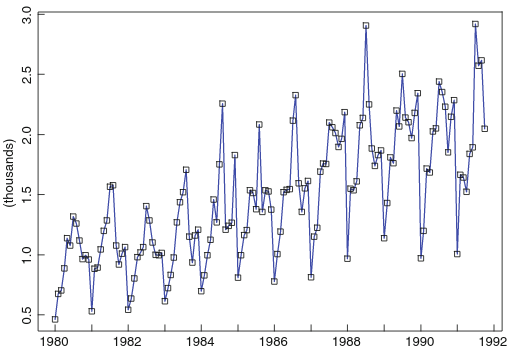
\includegraphics[width=.6\textwidth]{ej-ts}
  \caption{Ejemplo de serie temporal continuo en tiempo discreto. Ventas de vino tinto en Australia 1980-1991.}
  \label{fig:ej-ts}
\end{figure}

\begin{definicion}[Serie temporal]
  Sea un proceso estocástico $\{X_t\}_{t \in T}$, con $X_t : (\Omega, \mathcal{A}, P) \to (E, \mathcal{B}_E), \, \forall t \in T$. Una serie temporal es una realización del proceso estocástico $\{x_t : x_t \in E, t \in T \}$
  \label{def:serie-temporal}
\end{definicion}

Tenemos en cuenta que al hacer una realización obtendremos siempre una cantidad de puntos finitos, que no es excluyente con el hecho de que venga de un proceso en tiempo continuo mientras se haga un muestreo correcto. Además, sea el proceso en tiempo discreto o continuo, generalmente se considera que los tiempos en los que se obtiene la muestra están separados uniformemente.

\subsection{Momentos}

El estudio de los procesos y de las series está profundamente ligado a la predicción de valores: si conseguimos modelar y captar la estructura del proceso podremos predecir valores para tiempos en el futuro. Sin embargo, en general necesitaremos conocer las distribuciones $n$-dimensionales del proceso dadas por la distribución de probabilidad conjunta \eqref{eq:distri-multidim}

\begin{equation}
  P[X_{t_1} \leq x_{t_1}, \ldots, X_{t_n} \leq x_{t_n}], \; \forall \{t_i\}^n_{i = 1} \subseteq T, \; \forall n \in \N.
  \label{eq:distri-multidim}
\end{equation}

Esto en la práctica es muy complicado y poco fáctible de obtener, ya que usualmente solo se tiene una única serie temporal del proceso. Una manera más fácil y útil de describir un proceso es mediante los \textbf{momentos}, en particular los momentos de primer y segundo orden que son las funciones \textbf{media} (\autoref{def:func-media}) y \textbf{autocovarianza} (\autoref{def:func-autocovarianza}) respectivamente.

\begin{definicion}[Función media]
  Sea un proceso estocástico $\{X_t\}_{t \in T}$ que cumple que $E[X_t] < +\infty, \, \forall t \in T$. La función media del proceso se define como:

  $$\begin{aligned} \mu : T & \to \R \\
    t & \mapsto \mu(t) = E[X_t]
  \end{aligned}.$$
  \label{def:func-media}
\end{definicion}

\begin{definicion}[Función autocovarianza]
  Sea un proceso estocástico $\{X_t\}_{t \in T}$ que cumple que $Var[X_t] < +\infty, \, \forall t \in T$. La función media del proceso se define como:

  $$\begin{aligned} \gamma : T \times T & \to \R \\
    (t_1, t_2) & \mapsto \gamma(t_1, t_2) = E\left[(X_{t_1} - \mu(t_1))(X_{t_2} - \mu(t_2))\right] = Cov(X_{t_1}, X_{t_2})
  \end{aligned}.$$
  \label{def:func-autocovarianza}
\end{definicion}

Podemos definir la función \textbf{varianza} como un caso especial de la función autocovarianza cuando $t_1 = t_2$, es decir $\sigma^2(t) = \gamma(t_1, t_1) = Var[X_t]$.

\subsection{Procesos estacionarios}

Una propiedad muy interesante y que puede ayudarnos al modelar los procesos, es cuando es \textbf{estacionario}. De manera informal, un proceso es estacionario si sus propiedades estadísticas (momentos) no cambian con el tiempo.

Veamos que significa formalmente que un proceso sea \textbf{estrictamente estacionario} (\autoref{def:estrictamente-estacionario}).

\begin{definicion}[Proceso estrictamente estacionario]
  Un proceso estocástico $\{X_t\}_{t \in T}$ se dice que es estrictamente estacionario si $\forall n \in N$, $\forall t_1 < \ldots < t_n \in T$, $\forall \tau \in T$ se cumple que:

    $$\left( X_{t_1}, \ldots, X_{t_n}\right) \sim \left( X_{(t_1 + \tau)}, \ldots, X_{(t_n + \tau)}\right).$$
  \label{def:estrictamente-estacionario}
\end{definicion}

Lo que nos dice esta propiedad es que la probabilidad conjunta no cambia si se desplaza, por lo que solo dependerá de la probabilidad conjunta para $t_1, \ldots, t_n$, $\forall n \in N$. De hecho si $n=1$ tendremos que los momentos, si existen, serán todos iguales \eqref{eq:estricto-momentos}

\begin{gather}
  \mu(t) = \mu, \\
  \sigma^2(t) = \sigma^2.
  \label{eq:estricto-momentos}
\end{gather}

Además, si $n = 2$ entonces la distribución conjunta de $X_{t_1}$ y $X_{t_2}$ dependerá solo de la diferencia temporal $(t_2 - t_1) = \tau$ denominada como \textbf{desfase} (\emph{lag}). Por tanto la función autocovarianza puede ser reescrita en función únicamente del desfase, denominándose como \textbf{coeficiente de autocovarianza} con desfase $\tau$ \eqref{eq:estricto-autocovarianza}

\begin{equation}
  \gamma(t_1, t_2) = Cov(X_{t_1}, X_{t_2}) = Cov(X_{0}, X_{(t_2 - t_1)}) = \gamma(0, \tau) = \gamma(\tau).
  \label{eq:estricto-autocovarianza}
\end{equation}

Como las dimensiones del coeficiente de autocovarianza depende de las unidades de medida de $X_t$, por motivos de interpretabilidad se suele estandarizar obteniendo así la función de \textbf{autocorrelación} (ACF) que mide la correlación entre $X_t$ y $X_{t + \tau}$ \eqref{eq:autocorrelacion}

\begin{equation}
  \rho(\tau) = \dfrac{\gamma(\tau)}{\gamma(0)}.
  \label{eq:autocorrelacion}
\end{equation}

Aunque pareciera que no existen muchos procesos que mantengan la misma distribución en todo el tiempo, si existen muchos procesos con una distribución \textbf{de equilibrio}. Estos procesos cumplen que la distribución de probabilidad de $X_t$ tiende a una distribución limite (de equilibrio) cuando $t \to \infty$ y no dependen de las condiciones iniciales. Por tanto si las condiciones iniciales se fijan para ser iguales que la distribución de equilibrio, el proceso es fuertemente estacionario.

Sin embargo, podemos relajar las condiciones de la propiedad para hacerlas más prácticas en casos reales, únicamente con condiciones a los momentos de primer y segundo orden. Definimos los procesos \textbf{débilmente estacionarios} o \textbf{estacionarios de segundo orden} como \autoref{def:debilmente-estacionario}.

\begin{definicion}[Proceso estacionario de segundo orden]
  Sea un proceso estocástico $\{X_t\}_{t \in T}$, se dice que el proceso es débilmente estacionario o estacionario de segundo orden si se cumple lo siguiente:

  \begin{enumerate}
    \item $\mu(t) = \mu, \, \forall t \in T$.
    \item $\gamma(t_1, t_2) = \gamma  (t_1 + \tau, t_2 + \tau), \, \forall t_1, t_2, \tau \in T$
  \end{enumerate}

  La condición 2, como ya vimos, implica que $\gamma(t_1, t_2) = \gamma(\tau)$.
  \label{def:debilmente-estacionario}
\end{definicion}

Obviamente que un proceso sea fuertemente estacionario implica que sea débilmente estacionario pero no al revés. De hecho la doble implicación se da si el proceso tiene una distribución conjunta normal multivariante, ya que en ese caso queda determinada por los momentos de primer y segundo orden.

El \textbf{ruido independiente idénticamente distribuido} (ruido iid.) es el ejemplo básico de proceso estrictamente estacionario (\autoref{def:ruido-iid}).

\begin{definicion}[Ruido iid]
  Un proceso $\{X_t\}_{t \in T}$ estocástico se dice que es ruido independiente idénticamente distribuido con media $\mu$ y varianza $\sigma^2$, denotado por $\{X_t\} \sim IID(\mu, \sigma^2)$, si todas las variables aleatorias $X_t$ son independientes e idénticamente distribuidas con $E[X_t] = \mu, Var[X_t] = \sigma^2, \, \forall t \in T$.
\label{def:ruido-iid}
\end{definicion}

Debido a la independencia de las variables tendremos que la función media del proceso será $\mu$, y la función autocovarianza será \eqref{eq:autocov-ruido}

\begin{equation}
  \gamma(\tau) =
  \begin{cases}
    \sigma^2, & \tau = 0 \\
    0, & \tau \neq 0
  \end{cases},
  \label{eq:autocov-ruido}
\end{equation}

que no depende del tiempo $t$ y junto a la independencia de las variables nos dice que el proceso es estrictamente estacionario.

Uno puede relajar la condición de independencia e distribución idéntica para obtener un tipo de proceso estacionario de segundo orden, el llamado \textbf{ruido blanco} (\autoref{def:ruido-blanco}).

\begin{definicion}[Ruido blanco]
  Un proceso $\{X_t\}_{t \in T}$ estocástico se dice que es ruido blanco (\emph{white noise}) con media $\mu$ y varianza $\sigma^2$, denotado por $\{X_t\} \sim WN(\mu, \sigma^2)$, si todas las variables aleatorias $X_t$ son incorreladas con $E[X_t] = \mu, Var[X_t] = \sigma^2, \, \forall t \in T$.
\label{def:ruido-blanco}
\end{definicion}

En este caso el ruido blanco obtiene la misma función media y autocovarianza que el ruido iid. \eqref{eq:autocov-ruido} haciendo que el proceso sea estacionario de segundo orden. Así, cualquier proceso $IID(\mu, \sigma^2)$ es $WN(\mu, \sigma^2)$ pero no al revés.

Para ambos procesos podemos calcular la función de autocorrelación \eqref{eq:ruido-autocorrelacion}

\begin{equation}
  \rho(\tau) =
  \begin{cases}
    1, & \tau = 0 \\
    0, & \tau \neq 0
  \end{cases}.
  \label{eq:ruido-autocorrelacion}
\end{equation}

Mostramos un ejemplo de un proceso $\{X_n\}_{n = 1}^{500} \sim IID(0, 1)$ generado con $X_n \sim N(0, 1), \, n = 1, \ldots, 500$ junto con su correlograma (el valor de la función de autocorrelación en función del desfase) (\autoref{fig:ruido-ej}, \cite{chatfield2019analysis}).

\begin{figure}[htpb]
  \centering
  %\hspace*{-2.5cm}
  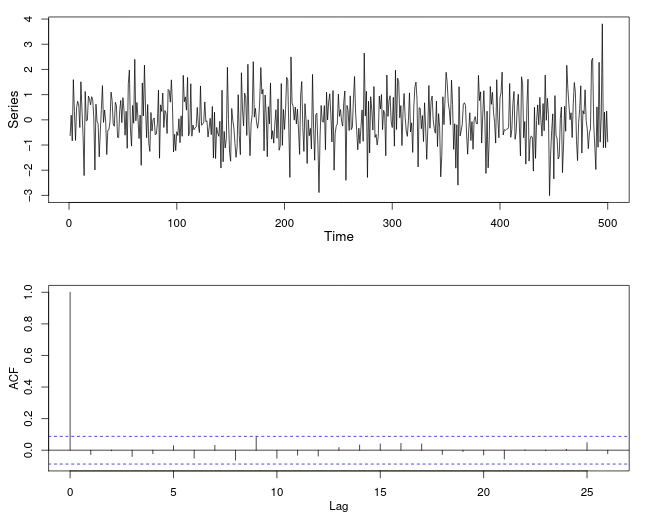
\includegraphics[width=.8\textwidth]{ruido-iid}
  \caption{Proceso $IID(0, 1)$ con su correlograma.}
  \label{fig:ruido-ej}
\end{figure}

Un proceso muy simple que no es estacionario es el \textbf{camino aleatorio} (\autoref{def:random-walk}).

\begin{definicion}[Camino aleatorio]
  Se dice que un proceso $\{X_t\}_{t \in T}$ es un camino aleatorio si

  $$X_t = X_{t - 1} + Z_t, \, \forall t \in T,$$

  donde $\{Z_t\}_{t \in T} \sim IID(\mu , \sigma^2)$. Generalmente cuando $t = 1$ se toma $X_1 = Z_1$, haciendo que el proceso sea como:

  $$X_t = \sum \limits^t_{i = 1} Z_i, \, \forall t \in T.$$
  \label{def:random-walk}
\end{definicion}

Para un camino aleatorio se tiene debido a la independencia de $Z_t$ que $E[X_t] = t \mu$ y $Var[X_t] = t \sigma^2$. Como dependen de $t$ el proceso no es estacionario.

Podemos generar caminos aleatorios fácilmente mediante un proceso $IDD(\mu, \sigma^2)$ (\autoref{fig:ej-random-walk}, \cite{chatfield2019analysis}).

\begin{figure}[htpb]
  \centering
  %\hspace*{-2.5cm}
  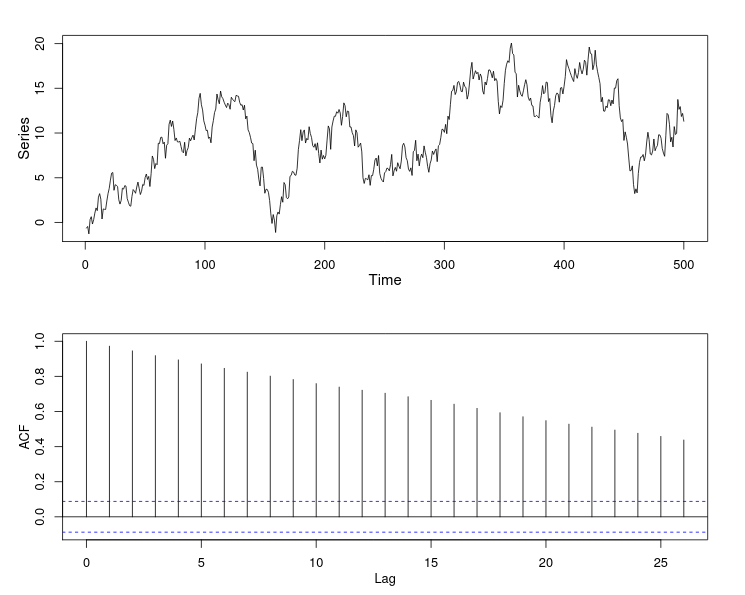
\includegraphics[width=.8\textwidth]{random-walk-ej}
  \caption{Ejemplo de camino aleatorio generado con ruido, junto con su correlograma.}
  \label{fig:ej-random-walk}
\end{figure}

\subsection{Propiedades de la funciones de autocovarianza y autocorrelación}

Finalmente veremos unas pocas propiedades interesantes sobre las funciones de autocovarianza $\gamma$ y autocorrelación $\rho$ de un proceso estacionario. Primero veamos las propiedades de la autocovarianza (\autoref{prop:propiedades-gamma}).

\begin{proposicion}[Propiedades de $\gamma$]
  Sea un proceso estacionario de segundo orden $\{X_t\}_{t \in T}$ con función de autocovarianza definida como

  $$\gamma(\tau) = Cov(X_{t + \tau}, X_t), \; \forall \tau \in T,$$

  entonces se cumplen las siguientes afirmaciones

  \begin{enumerate}
    \item $\gamma(0) = \sigma^2 \geq 0$.
    \item $|\gamma(\tau)| \leq \gamma(0), \, \forall \tau \in T$.
    \item $\gamma$ es par: $\gamma(\tau) = \gamma(-\tau), \, \forall \tau \in T$.
  \end{enumerate}
  \label{prop:propiedades-gamma}
\end{proposicion}

\begin{proof}
  La primera propiedad es consecuencia directa de que $Var[X_t] = \sigma^2 \geq 0, \, \forall t \in T$. Para la segunda aplicamos la desigualdad de Cauchy-Schwarz para el valor absoluto de la covarianza

    $$|\gamma(\tau)| = |Cov(X_{t+\tau}, X_t)| \leq \sqrt{Var[X_{t+\tau}]Var[X_t]} = \sqrt{\gamma(0)\gamma(0)} = \sqrt{\gamma(0)^2} = \gamma(0), \; \forall \tau \in T.$$

  Finalmente la tercera propiedad es inmediata

  $$\gamma(\tau) = Cov(X_{t + \tau}, X_t) = Cov(X_t, X_{t + \tau}) = \gamma(\tau), \; \forall \tau \in T.$$
\end{proof}

Como $\rho$ está definida en base a $\gamma$, las propiedades se siguen de estas (\autoref{prop:propiedades-rho}).

\begin{proposicion}[Propiedades de $\rho$]
  Sea un proceso estacionario de segundo orden $\{X_t\}_{t \in T}$ con función de autocorrelación definida como

  $$\rho(\tau) = \dfrac{\gamma(\tau)}{\gamma(0)} = \dfrac{\gamma(\tau)}{\sigma^2}, \; \forall \tau \in T,$$

  entonces se cumplen las siguientes afirmaciones

  \begin{enumerate}
    \item $\rho(0) = 1$.
    \item $|\rho(\tau)| \leq 1, \, \forall \tau \in T$.
    \item $\rho$ es par: $\rho(\tau) = \rho(-\tau), \, \forall \tau \in T$.
  \end{enumerate}
  \label{prop:propiedades-rho}
\end{proposicion}

\begin{proof}
  Todas se demuestran por consecuencia de las propiedades de $\gamma$: la primera ya que $\gamma(0) = \sigma^2$, y por tanto $\rho(0) = \gamma(0) / \sigma^2 = 1$. La segunda por $|\gamma(\tau)| \leq \sigma^2$ se tiene

  $$|\rho(\tau)| = \dfrac{|\gamma(\tau)|}{\sigma^2} \leq \dfrac{\sigma^2}{\sigma^2} = 1, \; \forall \tau \in T.$$

  Finalmente la tercera por ser $\gamma$ par tenemos

  $$\rho(\tau) = \dfrac{\gamma(\tau)}{\sigma^2} = \dfrac{\gamma(-\tau)}{\sigma^2} = \rho(-\tau), \; \forall \tau \in T.$$
\end{proof}

\section{Modelos estacionarios}

El objetivo del análisis de series es como encontrar en las series un proceso que sea estacionario para poder modelar correctamente simulaciones y predicciones de la serie.

Los dos enfoques principales para conseguir esto se basan en:

\begin{itemize}
  \item La descomposición de las series en varias componentes donde una de ellas son residuos que se esperan que sean estacionarios.
  \item La diferenciación de las series, restando los valores actuales con los valores anteriores hasta que la serie restante sea estacionaria.
\end{itemize}

En cualquier caso obtendremos un proceso estacionario que queremos modelar para poder predecir correctamente valores futuros. Para conseguir esto utilizaremos una clase de modelos lineales para las series temporales, como la clase de modelos de medias móviles autoregresivas (ARMA), que nos permitirá el estudio de los procesos estacionarios. De hecho veremos que cualquier proceso  estacionario de segundo orden o bien es un proceso lineal, o se puede transformar a uno mediante la eliminación de una componente determinista.

\subsection{Procesos de medias móviles}

Primero mostramos el proceso de \textbf{medias móviles} que construye el proceso tomando una combinación lineal de $q$ valores anteriores de un proceso de ruido (\autoref{def:media-movil}).

\begin{definicion}[Proceso de media móvil]
  Sea un proceso de ruido blanco $\{Z_t\}_{t \in T} \sim WN(0, \sigma^2)$ y constantes reales $\{\theta_t\}_{t = 0}^q \subset \R$. Se define el proceso de media móvil de orden $q$, denotado como $\{X\}_{t \in T} \sim MA(q)$, con la siguiente expresión:

  $$X_t = \theta_0 Z_t + \theta_1 Z_{t - 1} + \ldots + \theta_q Z_{t - q} = \sum \limits^q_{i = 0} \theta_i Z_{t - i}, \; \forall t \in T.$$
  \label{def:media-movil}
\end{definicion}

Es posible que el ruido tenga media $\mu$ distinta de cero, pero consideramos que es nula para simplificar el proceso. Si analicemos estos procesos, por un lado obtenemos inmediatamente al ser $Z_t$ incorreladas que \eqref{eq:media-media-auto}

\begin{gather}
  E[X_t] = 0, \\
  Var[X_t] = \sigma^2 \sum \limits^q_{i = 0} \theta_i^2.
  \label{eq:media-media-auto}
\end{gather}

También calculamos el coeficiente de autocovarianza \eqref{eq:media-coef-auto}

\begin{equation}
  \begin{aligned}
    \gamma(\tau) & = Cov(X_t, X_{t + \tau}) \\
    & = Cov\left(\sum \limits^q_{i = 0} \theta_i Z_i, \sum \limits^q_{i = 0} \theta_i Z_{t + \tau - i}\right) \\
    & = \begin{cases}
      0, & \tau > q \\
      \sigma^2 \sum \limits^{q - \tau}_{i = 0} \theta_i \theta_{i + \tau}, & 0 \leq \tau \leq q
    \end{cases}.
  \end{aligned}
\label{eq:media-coef-auto}
\end{equation}

Como $\gamma(\tau)$ no depende de $t$ y la media es constante, los procesos de media móvil son estacionarios de segundo orden para cualquier $q \in \N$ y $\{\theta_t\}_{t = 0}^q \subset \R$.

Finalmente veamos la función de autocorrelación \eqref{eq:media-autocor}

\begin{equation}
  \rho(\tau) = \begin{cases}
    1, & \tau = 0 \\
    \dfrac{\sum \limits^{q - \tau}_{i = 0} \theta_i \theta_{i + \tau}}{\sum \limits^q_{i = 0} \theta_i^2}, & 0 < \tau \leq q \\
    0, & \tau > q
  \end{cases}.
  \label{eq:media-autocor}
\end{equation}

De la construcción de estos modelos vemos que cada $X_t$ es dependiente de otros $X_s$ cuando $|\tau| = |t-s| \leq q$, es decir son $q$-dependientes y cuando $\tau > q$ entonces las variables son independientes. Una idea análoga se encuentra para los momentos de segundo orden, donde hablamos de procesos $q$-correlados. (\autoref{def:q-correlacion}).

\begin{definicion}[Proceso $q$-correlado]
  Un proceso estacionario $\{X\}_{t \in T}$ se dice que es $q$-correlado si se cumple lo siguiente:

  $$\gamma(\tau) = 0, \; \forall |\tau| > q$$.
  \label{def:q-correlacion}
\end{definicion}

Por \eqref{eq:media-media-auto} tenemos que un modelo $MA(q)$ es $q$-correlado, y de hecho la otra implicación se da también (\autoref{prop:q-correlado}, demostración en \cite{brockwell1991time} Sección 3.2)

\begin{proposicion}
  Sea un proceso estacionario de segundo orden $\{X_t\}_{t \in T}$ con media 0 y $q$-correlado. Entonces el proceso puede representarse como un modelo $MA(q)$.
\label{prop:q-correlado}
\end{proposicion}

Mediante ruido blanco $Z_t \sim N(0, 1)$ podemos construir modelos $MA$ fácilmente. Por ejemplo podemos construir un modelo $MA(1)$ definido por $X_t = Z_t - \frac{4}{5}Z_{t - 1}$ y otro $MA(2)$ dado por $X_t = Z_t + \frac{7}{10} Z_{t - 1} - \frac{1}{5}Z_{t - 2}$. Mostramos las series realizadas de estos procesos junto con sus correlogramas \autoref{fig:ej-media} (\cite{chatfield2019analysis}).

\begin{figure}[htpb]
  \centering
  %\hspace*{-2.5cm}
  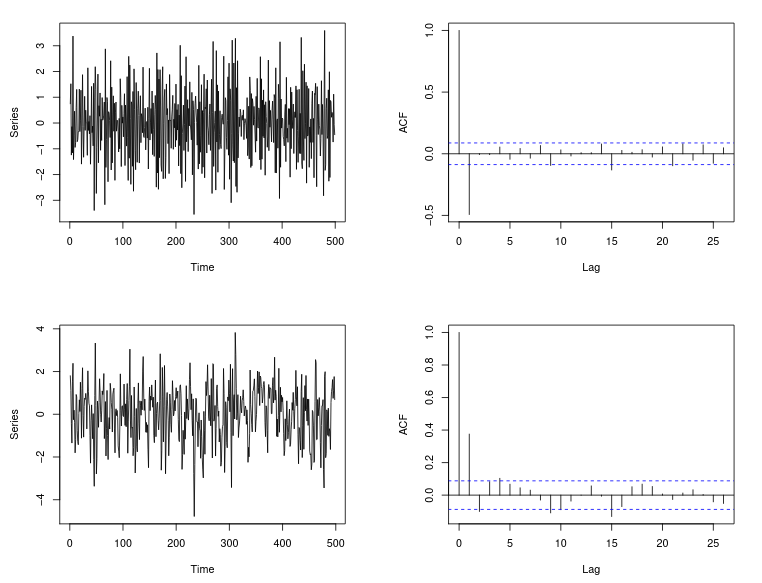
\includegraphics[width=.8\textwidth]{ej-media}
  \caption{Ejemplos de $MA(1)$ (arriba) y $MA(2)$ (abajo) con sus correlogramas respectivos a la derecha.}
  \label{fig:ej-media}
\end{figure}

Observamos como para $MA(1)$ el correlograma muestra valores significativos solo para $\tau = 0, 1$ y para $MA(2)$ para $\tau = 0, 1, 2$, correspondiéndose con nuestro estudio de la función de autocorrelación.

\subsection{Procesos autorregresivos}

Consideramos un modelo que se basa en la idea de las medias móviles de utilizar valores de tiempos pasados, pero en vez de considerarlas de un proceso basado en ruido usaremos el propio proceso (\autoref{def:proceso-autorregresivo}).

\begin{definicion}[Proceso autorregresivo]
  Un proceso $\{X_t\}_{t \in T}$ se dice que es un proceso autorregresivo de orden $p$, notado como $\{X_t\} \sim AR(p)$, si se puede expresar de la siguiente forma:

  $$X_t = \phi_1 X_{t-1} + \ldots + \phi_p X_{t - p} + Z_t = \sum \limits^p_{i = 1} \left(\phi_i X_{t - i}\right) + Z_t, \; \forall t \in T,$$

  donde $\{Z_t\}_{t \in T} \sim WN(0, \sigma^2)$, y coeficientes reales $\{\phi_i\}_{i = 1}^p \subset \R$.
  \label{def:proceso-autorregresivo}
\end{definicion}

Se ha considerado que $\mu = 0$, aunque es posible trabajar con una media no nula. Así, estudiamos el caso más simple $p = 1$, $AR(1)$ expresado como \eqref{eq:ar-simple}

\begin{equation}
  X_t = \phi X_{t - 1} + Z_t, \, \forall t \in T.
  \label{eq:ar-simple}
\end{equation}

Si sustituimos los $X_{t - i}$ mediante recursividad obtenemos \eqref{eq:ar-simple2}

\begin{equation}
  X_t = \phi\left(\phi X_{t-2} + Z_{t-1}\right) + Z_t = \phi^2\left(\phi X_{t-3} + Z_{t-2}\right) + \phi Z_{t-1} + Z_t, \, \forall t \in T.
  \label{eq:ar-simple2}
\end{equation}

Si repetimos este proceso infinitamente entonces \eqref{eq:ar-simple3}

\begin{equation}
  X_t = Z_t + \phi Z_{t-1} + \phi^2 Z_{t-2} + \ldots = \sum \limits^{+\infty}_{i = 0} \phi^i Z_{t - i}, \; \forall t \in T,
  \label{eq:ar-simple3}
\end{equation}

escogido $|\phi| < 1$ para que la suma converja, $AR(1)$ se comporta como un modelo $MA(\infty)$, indicando que hay una cierta dualidad entre los modelos $AR$ y $MA$.

Estudiamos el primer y segundo orden del proceso considerando que las variables $Z_t$ son incorreladas, entonces $\forall t \in T$ se tiene \eqref{eq:ar-momentos}

\begin{gather}
  E[X_t] = 0, \\
  Var[X_t] = \sigma^2 \sum \limits^{+\infty}_{i = 0} \left(\phi^{2i}\right).
  \label{eq:ar-momentos}
\end{gather}

La varianza será finita si $|\phi|^2 < 1$, por lo que al tomar $|\phi| < 1$ se tiene \eqref{eq:ar-var}

\begin{equation}
  Var[X_t] = \dfrac{\sigma^2}{1 - \phi^2}, \; \forall t \in T.
  \label{eq:ar-var}
\end{equation}

La función de autocovarianza viene dada por \eqref{eq:ar-autocovarianza}

\begin{equation}
  \begin{aligned}
    \gamma(\tau) & = E[X_t X_{t + k}] = E\left[\left(\sum \limits^{+\infty}_{i = 0} \phi^i Z_{t - i}\right)\left(\sum \limits^{+\infty}_{i = 0} \phi^i Z_{t + \tau - i}\right)\right] \\
    & = \sigma^2 \sum \limits^{+\infty}_{i = 0} \phi^i \phi^{\tau + i} = \phi^\tau \dfrac{\sigma^2}{1 - \phi^2}.
  \end{aligned}
  \label{eq:ar-autocovarianza}
\end{equation}

Por tanto como $\gamma(\tau)$ no depende de $t$, el proceso $AR(1)$ es un proceso estacionario de segundo orden (bajo la condición de que $|\phi| < 1$). La función de autocorrelación será \eqref{eq:ar-autocorrelacion}

\begin{equation}
  \rho(\tau) = \phi^\tau, \; \tau \in T.
  \label{eq:ar-autocorrelacion}
\end{equation}

Simulemos unos cuantos procesos autorregresivos mediante ruido $Z_t \sim N(0, 1)$: $X_t = \frac{4}{5}X_{t-1} + Z_t$, $X_t = -\frac{4}{5}X_{t-1} + Z_t$ y $X_t = \frac{3}{10}X_{t-1} + Z_t$ cuyas series mostramos de arriba a bajo respectivamente, junto a sus correlogramas en \autoref{fig:ar-simulado} (\cite{chatfield2019analysis}).

\begin{figure}[htpb]
  \centering
  %\hspace*{-2.5cm}
  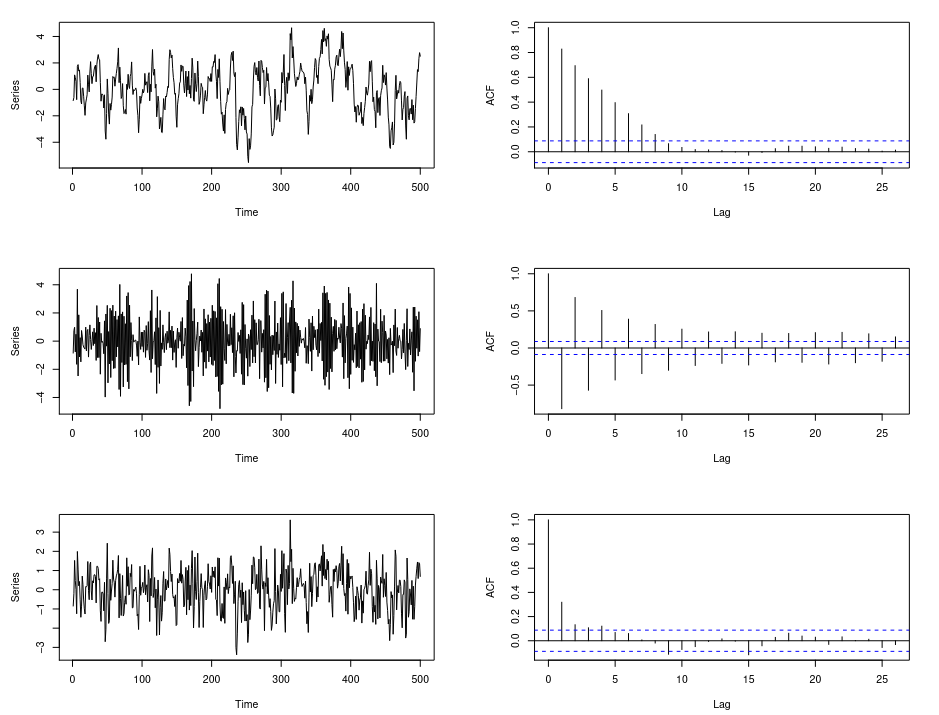
\includegraphics[width=.85\textwidth]{ar-simulado}
  \caption{Ejemplos de $AR(1)$ con varios valores junto con sus correlogramas.}
  \label{fig:ar-simulado}
\end{figure}

Observamos como los correlogramas van convergiendo a 0, decreciendo absolutamente. Cuando $1 > \phi > 0$ (1er y 3er proceso) los valores son todos positivos mientras que cuando $-1 < \phi < 0$ (2o proceso) se van alternando entre positivos (desfase par) y negativos (desfase negativo).

Por otro lado, la función de autocovarianza \eqref{eq:ar-autocovarianza} era posible obtenerla de otra manera. Asumimos de antemano que el proceso es estacionario, entonces $E[X_t]$ debe ser constante (asumamos que es 0). Si multiplicamos el modelo \eqref{eq:ar-simple} por $X_{t-k}$ y tomamos esperanzas obtenemos \eqref{eq:ar-truco}

\begin{equation}
  \gamma(\tau) = \phi \gamma(-\tau + 1), \; \forall \tau > 0,
  \label{eq:ar-truco}
\end{equation}

ya que $E[Z_t X_{t-\tau}] = 0$, $\forall \tau > 0$ debido a la incorrelación de las $Z_t$. Además como $\gamma$ es función par entonces \eqref{eq:ar-truco2}

\begin{equation}
  \gamma(\tau) \phi \gamma(\tau - 1), \; \forall \tau > 0.
  \label{eq:ar-truco2}
\end{equation}

Finalmente como $\gamma(0) = \sigma^2_X$ entonces $\gamma(\tau) = \phi^\tau \sigma^2_X, \; \forall \tau \geq 0$ y además $\rho(\tau) = \phi^\tau, \; \forall \tau > 0$.

Recordando una de las propiedades de $\rho$ cuando el proceso era estacionario se tenía que $|\rho(\tau)| \leq 1, \, \forall \tau \geq 0$ entonces se debe cumplir que $|\phi| \leq 1$. Excluimos el caso degenerado $|\phi| = 1$ y por tanto se debe cumplir que $|\phi| < 1$.

Esta forma alternativa es aplicable para el caso de un modelo $AR(p)$ general, obteniendo Las siguiente ecuaciones para la función de autocorrelación \eqref{eq:ar-general}

\begin{equation}
  \rho(\tau) = \phi_1 \rho(\tau - 1) + \cdots + \phi_p \rho(\tau - p) =
  \begin{cases}
    \sigma^2, & \tau = 0 \\
    0, & 0 < \tau \leq p
  \end{cases}
  \label{eq:ar-general}
\end{equation}

Estas son las llamadas ecuaciones de Yule-Walker \cite{yule1971method, walker1931periodicity}, un conjunto de ecuaciones en diferencias que tienen la solución general \eqref{eq:sol-general}

\begin{equation}
  \rho(\tau) = A_1 \pi_1^{|\tau|} + \cdots + A_p \pi_p^{|\tau|}, \; \forall \tau > 0,
  \label{eq:sol-general}
\end{equation}

donde $\{\pi_i\}_{i = 0}^p$ son las raíces de la ecuación auxiliar \eqref{eq:sol-auxiliar}

\begin{equation}
  y^p - \phi_1 y^{p-1} - \cdots - \phi_p = 0.
  \label{eq:sol-auxiliar}
\end{equation}

Las constantes $\{A_i\}_{i = 0}^p$ se escogen para satisfacer las condiciones iniciales dependientes de $\rho(0) = 1$, que implican que $\sum_{i = 0}^p A_i = 1$. Las $(p - 1)$ primeras ecuaciones de Yule-Walker añaden $(p-1)$ restricciones más en $\{A_i\}_{i = 0}^p$ usando $\rho(0) = 1$ e $\rho(\tau) = \rho(\tau)$.

De la solución \eqref{eq:sol-general} vemos que $\rho(\tau)$ no depende de $t$ por lo que lo único que necesitamos para que el proceso $AR(p)$ sea estacionario es que los $|\pi_i| < 1$, $i = 1, \ldots, p$, que de hecho es una condición necesaria y suficiente.

\subsection{Procesos lineales}

Si generalizamos el funcionamiento de los modelos $AR$ y $MA$ llegamos a los procesos lineales (\autoref{def:proceso-lineal}).

\begin{definicion}[Proceso lineal]
  Un proceso $\{X\}_{t \in T}$ se dice que es un proceso lineal si se puede representar de la siguiente forma:

  $$X_t = \sum \limits^{+\infty}_{i = -\infty} \psi_{j} Z_{t - i}, \; \forall t \in T,$$

  con $\{Z\}_{t \in T} \sim WN(0, \sigma^2)$ y $\{\psi_i\}^{+\infty}_{i = -\infty} \subset \R$ constantes que cumplen que $\sum \limits^{+\infty}_{i = -\infty} |\psi_j| < \infty$.
  \label{def:proceso-lineal}
\end{definicion}

Según los coeficientes $\psi$ se puede obtener cualquier modelo $AR$ o $MA$. Por ejemplo si se toman $\psi = 0, \, \forall i < 0$ entonces el proceso sería $MA(\infty)$.

Veamos entonces que si cualquier proceso lineal es estacionario de segundo orden si lo es el proceso $\{Z_t\}_{t \in T}$, de manera que cualquier proceso $AR$ o $MA$ será estacionario de segundo orden (\autoref{prop:proceso-estacionario}).

\begin{proposicion}
  Sea $\{Y_t\}_{t \in T}$ un proceso estacionario de segundo orden con media 0 y función de autocovarianza $\gamma_Y$. Si $\sum_{i = -\infty}^{+\infty} |\psi_i| < \infty$, entonces el proceso definido por:

  $$X_t = \sum \limits^{+\infty}_{i = -\infty} \psi_i Y_{t - i},$$

  es estacionario de segundo orden con media 0 y función de autocovarianza

  $$\gamma_X(\tau)= \sum \limits^{+\infty}_{i=-\infty}\sum \limits^{+\infty}_{j = -\infty} \psi_i \psi_j \gamma_Y(\tau + j - i), \, \tau \in T.$$

  De hecho si $\{X_t\}_{t \in T}$ es un proceso lineal, se tiene que

  $$\gamma_X(\tau) = \sum \limits^{+\infty}_{i = -\infty} \psi_{i} \psi_{i + \tau}\sigma^2, \, \tau \in T.$$
  \label{prop:proceso-estacionario}
\end{proposicion}

\begin{proof}
  Debido a que la suma absoluta de los coeficientes es finita podemos asegurar que la suma $X_t$ es convergente, $\forall t \in T$ se cumple que

  $$E[|X_t|] \leq \sum \limits^{+\infty}_{i = -\infty} |\psi_j| E[|Y_{t-i}|] \leq \sum \limits^{+\infty}_{i = -\infty} \left(|\psi_j|\right) \sqrt{\gamma_Y(0)} < \infty$$

  Como $E[Y_t] = 0, \, \forall t \in T$ Entonces

  $$E[X_t] = E\left[\sum \limits^{+\infty}_{i = -\infty} \psi_i Y_{t - i}\right] = \sum \limits^{+\infty}_{i = -\infty} \psi_i E[Y_{t-i}] = 0$$

  y además para $\tau \in T$

  $$\begin{aligned}
    E[X_{t+\tau}X_t] & = E\left[\left(\sum \limits^{+\infty}_{i = -\infty} \psi_i Y_{t + \tau - i}\right)\left(\sum \limits^{+\infty}_{i = -\infty} \psi_i Y_{t -i}\right)\right] \\
    & = \sum \limits^{+\infty}_{i = -\infty} \sum \limits^{+\infty}_{j = -\infty} \psi_i \psi_j E[Y_{t+\tau-i}Y_{t-j}] \\
    & = \sum \limits^{+\infty}_{i = -\infty}  \sum \limits^{+\infty}_{j = -\infty} \psi_i \psi_j \gamma_Y(\tau + j - i),
  \end{aligned}$$

  que no depende de $t$ y por tanto $\{X_t\}$ es estacionario de segundo orden. Finalmente si $\{Y_t\}$ es ruido blanco entonces $\gamma_Y(\tau + i - j) = \sigma^2$ si $j = i - \tau$ y 0 en caso contrario, obteniendo el último resultado.
\end{proof}

\subsection{Descomposición de Wold}

Recordemos que estamos con procesos estocásticos, en los que esperamos que haya una cierta componente probabilística. No vamos a definir exactamente cuando un proceso es \textbf{determinista} o \textbf{no determinista} ya que se necesitan conceptos muy complejos. En líneas generales nos vienen a indicar si existe cierta aleatoriedad en el proceso, o bien ya sabemos con seguridad absoluta el resultado que se va a obtener.

En todos los modelos que consideramos siembre buscamos que sean procesos no deterministas y no nos interesan los que sean deterministas. Mediante la descomposición de Wold veremos que cualquier serie estacionaria no determinista se puede expresar de manera única como un proceso que puede convertirse en un proceso lineal (\autoref{th:wold}, \cite{wold1938decomposition})

\begin{teorema}[Descomposición de Wold]
  Sea $\{X_t\}_{t \in T}$ un proceso no determinista estacionario de segundo orden, entonces el proceso se puede descomponer de manera única con los procesos $\{Z_t\}_{t \in T}$, $\{V_t\}_{t \in T}$ y coeficientes $\{\psi_i\}_{i = 0}^{\infty}$ de la siguiente forma

  $$ X_t = \sum \limits^{+\infty}_{i = 0} \psi_i Z_{t - i} + V_t, \, \forall t \in T,$$

  y además se cumple lo siguiente

  \begin{enumerate}
    \item $\psi_0 = 1$ y $\sum^{+\infty}_{i = 0} \psi^2_i < \infty$.
    \item $\{Z_t\}_{t \in T} \sum WN(0, \sigma^2)$.
    \item $Cov(Z_s, V_t) = 0$, $\forall t,s \in T$.
    \item $\{V_t\}$ es un proceso determinista.
  \end{enumerate}
  \label{th:wold}
\end{teorema}

El teorema incluye más condiciones que se cumplen pero se ha simplificado para su mejor entendimiento. Lo que nos expresa el teorema, es que cualquier proceso no determinista se puede representar como un proceso lineal que tiene añadido una parte determinista.

De hecho, esta parte determinista está asociada a la media del proceso por lo que para muchos procesos que ya tienen media 0 entonces nos quedará únicamente un proceso lineal \textbf{puramente determinista}.

\subsection{Procesos ARMA}

Finalmente introducimos uno de los procesos más importantes en el modelado de series temporales: los procesos ARMA (modelos autorregresivos de media móvil). La gran importancia de estos modelos reside en que para una clase grande de funciones de autocovarianza $\gamma$ es posible encontrar un proceso ARMA cuya función de autocovarianza $\gamma_X$ está aproximada.

Este modelo está formado combinando los dos modelos que hemos considerado, $MA$ y $AR$ (\autoref{def:arma}, \cite{whittle1951arma}).

\begin{definicion}[Proceso ARMA]
  Un proceso $\{X_t\}_{t \in T}$ se dice que es un proceso $ARMA(p, q)$ si $\{X_t\}$ es estacionario y se cumple que

  $$X_t = \psi X_{t-1} + \ldots + \psi_p X_{t-p} + Z_t + \theta_1 Z_{t-1} + \ldots + \theta_q Z_{t - q}, \; \forall t \in T,$$

  donde $\{Z_t\}_{t \in T} \sim WN(0, \sigma^2)$ y además los polinomios $\phi(z) = 1 - \phi_1 z - \ldots - \phi_p z^p$ y $\theta(z) = 1 + \theta_1z + \ldots + z_q z^q$ no tienen factores comunes.
\label{def:arma}
\end{definicion}

La condición de que los polinomios no tengan factores comunes se impone para que el modelo no se pueda reducir a uno más simple, así evitamos parámetros redundantes.

Si un modelo $ARMA(p, q)$ cumple que $p = 0$ o que $\phi_i = 0, \, \forall i = 1, \ldots, p$ entonces se convierte en un modelo $MA(q)$. Por el contrario si $q = 0$ o $\theta_i = 0, \, \forall i = 1, \ldots, q$, entonces el modelo sería un $AR(q)$.

En la definición vemos que es esencial que $\{X_t\}$ sea estacionario, haciendo un estudio del proceso se obtiene un teorema que nos asegura la existencia y unicidad con una condición muy simple (\autoref{th:existencia-unicidad-arma}, demostración en \cite{brockwell2002introduction} Sección 3.1).

\begin{teorema}[Existencia y unicidad de ARMA]
  Existe una solución estacionaria $\{X_t\}_{t \in T}$ para el modelo $ARMA(p, q)$, y además es la única, si y solo si

  $$\phi(z) = 1 - \phi_1 z - \cdots - \phi_p z^p \neq 0, \; \forall |z| = 1.$$
  \label{th:existencia-unicidad-arma}
\end{teorema}

Para calcular las funciones de autocovarianza y autocorrelación se vuelve a utilizar el método de las ecuaciones de Yule-Walker, donde la diferencia con los modelos $AR(p)$ reside en que tiene condiciones iniciales diferentes. También es posible utilizar el resultado \autoref{prop:proceso-estacionario}.

Mostramos dos ejemplos simulados de procesos $ARMA$, uno $ARMA(1,1)$ expresado como $X_t = \frac{7}{10}X_{t-1} + Z_t - \frac{2}{5}Z_{t-1}$ con $Z-t \sim N(0, 1)$ y otro $ARMA(2,2)$ con $X_t = \frac{9}{10}X_{t-1} - \frac{1}{2}X_{t-2} + Z_t - \frac{1}{5}Z_{t-1} + \frac{1}{4}Z_{t-2}$ con $Z_t \sim N(0, \frac{1}{2})$ en \autoref{fig:arma-ej} (\cite{chatfield2019analysis}).

\begin{figure}[htpb]
  \centering
  %\hspace*{-2.5cm}
  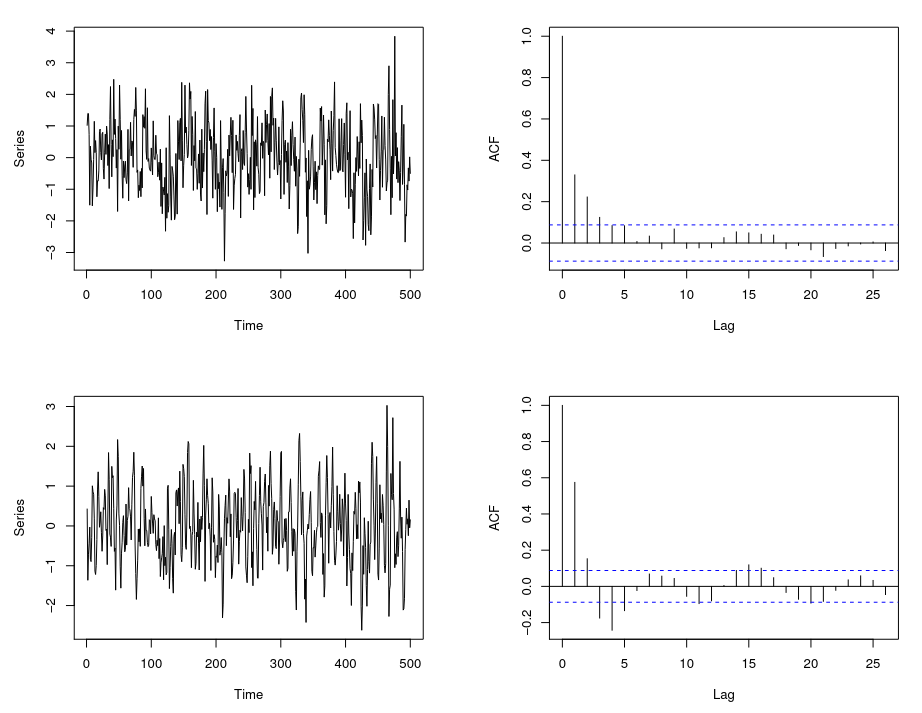
\includegraphics[width=.85\textwidth]{arma-ej}
  \caption{Ejemplos $ARMA(1,1)$ (arriba) y $ARMA(2,2)$ (abajo) con sus correlogramas.}
  \label{fig:arma-ej}
\end{figure}

Hemos obtenido un modelo muy potente con el que podemos adaptar con los parámetros $p$ y $q$ según la serie observada y la función de autocorrelación estimada.

No entraremos en detalles para la realización de predicciones con un modelo $ARMA(p,q)$ debido al largo y complejo desarrollo que debe hacerse, tanto como la estimación de parámetros $\{\phi_i\}$, $\{\theta_i\}$ para adaptar el modelo a la serie observada, como el cálculo de predicciones en base al modelo.

\section{Descomposición}

Una parte importante del análisis de series se centra en el modelado de los procesos mediante la descomposición en varias componentes que suelen exhibir, obteniendo una parte estacionaria al que aplicaremos los modelos vistos. Veremos cuáles son estas componentes y distintas maneras para obtener esta descomposición.

\subsection{Patrones}

Listemos los patrones fundamentales que muestran muchas series:

\begin{itemize}
  \item \textbf{Tendencia}: un cambio a largo plazo en el nivel medio de la serie, que puede ser creciente o decreciente.
  \item \textbf{Variación estacional}: un patrón que se repite cada cierto periodo de tiempo fijo debido a factores estacionales (cada estación, o año).
  \item \textbf{Variaciones cíclicas}: fluctuaciones de las series sin frecuencia fija y que pueden cambiar a lo largo del tiempo.
\end{itemize}

Veamos ejemplos de estos patrones en \autoref{fig:patrones-ej} \cite{hyndman2018forecasting}.

\begin{figure}[htpb]
  \centering
  %\hspace*{-2.5cm}
  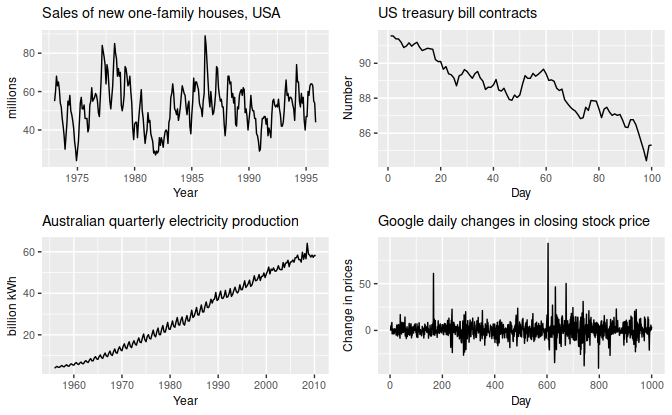
\includegraphics[width=.9\textwidth]{patrones-ejemplos}
  \caption{Ejemplos de series con distintos patrones.}
  \label{fig:patrones-ej}
\end{figure}

Analicemos cada serie para observar los patrones en cada una:

\begin{itemize}
  \item Arriba-izquierda: se muestra un carácter estacional cada año, junto con patrones cíclicos que van variando.
  \item Arriba-derecha: únicamente tendencia decreciente.
  \item Abajo-izquierda: tendencia creciente junto a una variación estacional de un año.
  \item Abajo-derecha: sin ningún patrón observable, son fluctuaciones aleatorias.
\end{itemize}

En base a estos patrones, el análisis clásico de series temporales se basa en la descomposición de estas en los componentes que hemos comentado \eqref{eq:decomposition}

\begin{equation}
  X_t = m_t + s_t + Y_t, \, \forall t \in T,
  \label{eq:decomposition}
\end{equation}

donde $m_t$ es la componente de la tendencia-ciclos (que se dice solamente tendencia), $s_t$ la componente estacional e $Y_t$ ruido aleatorio (débilmente) estacionario.

Esta descomposición se dice que es \textbf{aditiva} pues suma sus componentes y existe otra forma llamada \textbf{multiplicativa}, que suele ser útil cuando las fluctuaciones de la serie son proporcionales al tiempo de la serie \eqref{eq:decomposition-mult}

\begin{equation}
  X_t = m_t \cdot s_t \cdot Y_t, \, \forall t \in T.
  \label{eq:decomposition-mult}
\end{equation}

El enfoque de realizar la descomposición consiste en extraer de las series estas componentes $m_t$, $s_t$ y esperar que el ruido $Y_t$ sea estacionario. Crearemos así un modelo para el proceso estacionario en el que podemos simular valores junto con $m_t$ y $s_t$.

\subsection{Descomposición sin estacionalidad}

Si tenemos un proceso que no presenta la componente estacional entonces obtenemos el siguiente modelo (\autoref{def:solo-tendencia}).

\begin{definicion}[Descomposición con solo tendencia]
  Sea $\{X_t\}$ un proceso entonces una descomposición con solo tendencia está definida por:

  $$ X_t = m_t + Y_t, \; \forall t \in T,$$

  donde $m_t$ es la tendencia e $Y_t$ los residuos y se tiene que $E[Y_t] = 0, \forall t \in T$. Si esto último no fuese así, el modelo se cambiaría por:

  $$ X_t = (m_t + E[Y_t]) + (Y_t - E[Y_t]), \; \forall t \in T.$$
  \label{def:solo-tendencia}
\end{definicion}

\subsubsection{Ajuste polinómico}

Para poder estimar la tendencia $m_t$ podemos utilizar varias técnicas. La primera de ellas es la más simple y conocida: el \textbf{ajuste polinómico} (\autoref{def:ajuste-polinomico}).

\begin{definicion}[Ajuste polinómico]
  Sea un $\{X_t\}_{t = 1}^n$ un proceso y $\{x_t\}_{t = 1}^n$ una serie temporal observada del proceso. El ajuste polinómico de gradp $k$ considera que la tendencia es un polinomio de grado $k$ de la forma

  $$m_t = \sum \limits^k_{i = 0} a_i t^i,$$

  La tendencia estimada $\hat{m}_t$ determinada por los parámetros $\hat{a}_0, \hat{a}_1, \ldots, \hat{a}_k$ se obtienen al minimizar el error cuadrático medio $$\sum \limits^n_{t = 1} (x_t - m_t)^2.$$
  \label{def:ajuste-polinomico}
\end{definicion}

\autoref{fig:ajuste-ej} (\cite{brockwell2002introduction}) nos muestra un ejemplo de ajuste polinómico de grado 2 (cuadrático) donde se estima $\hat{m}_t = \hat{a}_0 + \hat{a}_1 t + \hat{a}_2 t^2$ a través de la serie observada.

\begin{figure}[htpb]
  \centering
  %\hspace*{-2.5cm}
  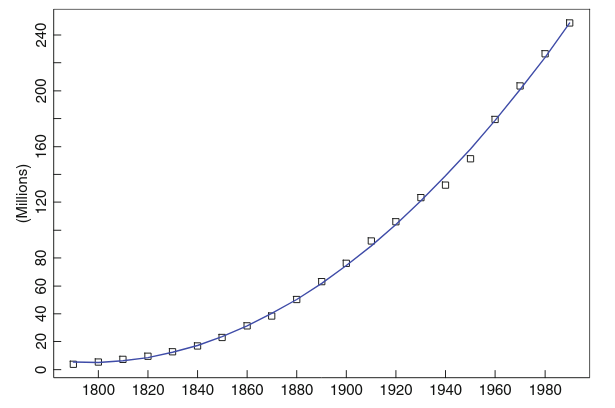
\includegraphics[width=.6\textwidth]{ajuste-ej}
  \caption{Ajuste cuadrático de la población en EE.UU. entre 1790-1990.}
  \label{fig:ajuste-ej}
\end{figure}

\subsubsection{Suavizado con media móvil}

La siguiente técnica consiste en estimar la tendencia mediante el \textbf{suavizado con media móvil} que está basado en el modelo de media móvil (\autoref{def:suavizacion-media}).

\begin{definicion}[Suavizado con media móvil]
  Sea un proceso $\{X_t\}_{t = 1}^n$, y un natural $q \in N$. Se define el proceso suavizado con media móvil simétrica de orden $q$ de $\{X_t\}$ como:

  $$ W_t = \dfrac{1}{2q + 1} \sum \limits^q_{i = -q} X_{t - i}, \, \forall t = 1, \ldots, n.$$
  \label{def:suavizacion-media}
\end{definicion}

Asumiendo que $m_t$ es aproximadamente lineal en el intervalo $[t - q, t + q]$ y que la media de los errores en el mismo intervalo es aproximadamente cero, aplicamos el suavizado al modelo \autoref{def:solo-tendencia} obteniendo \eqref{eq:suavizacion}

\begin{equation}
  W_t = \dfrac{1}{2q + 1} \sum \limits^q_{i = -q} m_{t - i} + \dfrac{1}{2q + 1} \sum \limits^q_{i = -q} Y_{t - i} \approx m_t, \; t = q + 1, \ldots, n - q.
  \label{eq:suavizacion}
\end{equation}

Por tanto la tendencia estimada para un proceso $\{X_t\}_{t = 1}^n$ quedaría como \eqref{eq:suavizacion-estimada}

\begin{equation}
  \hat{m}_t = \dfrac{1}{2q + 1} \sum \limits^q_{i = -q} X_{t - i}, \; t = q + 1, \ldots, n - q.
  \label{eq:suavizacion-estimada}
\end{equation}

Notamos que $\hat{m}_t$ no está definida para $t > n - q$ o $t \leq q$ que podría dejarse así o extender los términos definiendo $X_t := X_1, \forall t < 1$ y $X_t := X_n, \forall t > n$.

Un ejemplo de $\hat{m}_t$ aplicando un suavizado de media móvil con $q = 2$ (5 términos) lo tenemos en \autoref{fig:ej-suavizacion} (\cite{brockwell2002introduction}).

\begin{figure}[htpb]
  \centering
  %\hspace*{-2.5cm}
  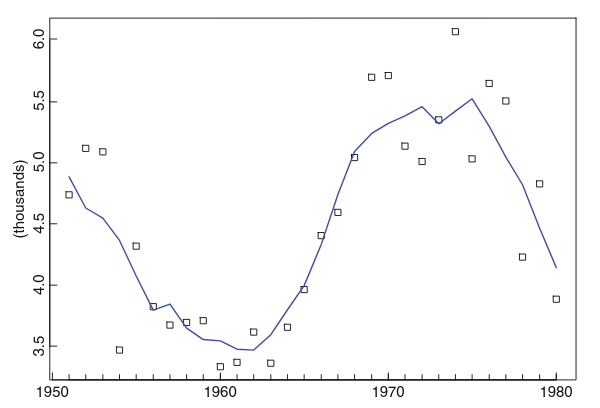
\includegraphics[width=.6\textwidth]{ej-suavizacion}
  \caption{Suavizado con media móvil con 5 términos del número de huelgas en EE.UU entre 1951-1980.}
  \label{fig:ej-suavizacion}
\end{figure}

\subsubsection{Suavizado exponencial}

Finalmente consideramos una técnica que realiza el suavizado como una combinación entre el punto $t$-ésimo actual y el punto estimador anterior (\autoref{def:suavizado-exponencial}).

\begin{definicion}[Suavizado exponencial]
  Sea $\{X_t\}_{t = 1}^n$ un proceso y $\alpha \in [0, 1]$, el suavizado exponencial se define como la estimación de la tendencia del proceso de la siguiente forma:

  $$\hat{m}_t = \alpha X_t + (1 - \alpha)\hat{m}_{t - 1}, \; t = 2, \ldots, n,$$

  donde $\hat{m}_1 = X_1$.
  \label{def:suavizado-exponencial}
\end{definicion}

Este método se denomina suavizado exponencial debido a que $\forall t \geq 2$ se cumple \eqref{eq:exponencial-desarrollada}

\begin{equation}
  \hat{m}_t = \sum \limits^{t - 2}_{i = 1} \alpha(1 - \alpha)^i X_{t - i} + (1 - \alpha)^{t - 1} X_1,
  \label{eq:exponencial-desarrollada}
\end{equation}

donde se puede ver el proceso estimado como una media móvil con pesos decrecientes exponencialmente. Un ejemplo lo tenemos en \autoref{fig:ej-suavizado} (\cite{brockwell2002introduction})

\begin{figure}[htpb]
  \centering
  %\hspace*{-2.5cm}
  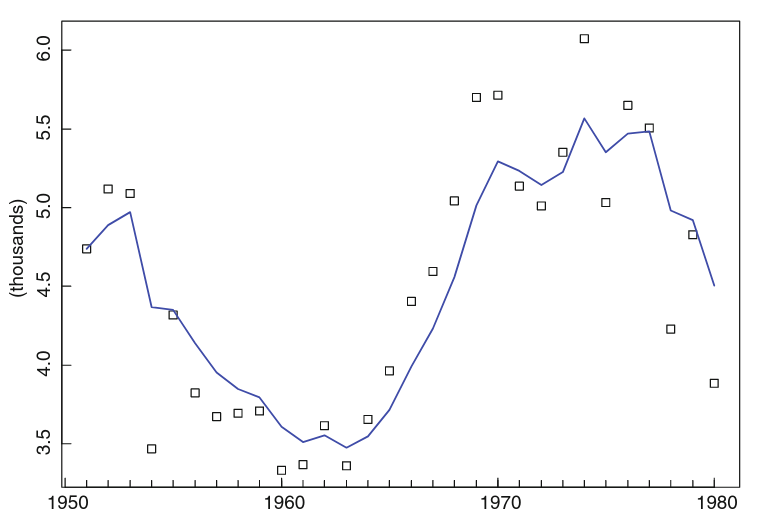
\includegraphics[width=.6\textwidth]{ej-suavizado}
  \caption{Suavizado exponencial con $\alpha = 0.6$ en el número de huelgas.}
  \label{fig:ej-suavizado}
\end{figure}

\subsection{Descomposición completa}

Ahora consideramos la descomposición completa, añadiendo al modelo que hemos estado utilizando la componente estacional. Esperamos que esta componente se repita siempre cada cierto periodo de tiempo $S$ y además que la suma de los valores en un periodo sea cero (\autoref{def:descomposicion-entera}).

\begin{definicion}[Descomposición completa]
  Sea $\{X_t\}$ un proceso entonces una descomposición completa está definida por:

  $$ X_t = m_t + s_t + Y_t, \; \forall t \in T,$$

  donde $m_t$ es la tendencia, $s_t$ es la estacionalidad con periodo $S$ e $Y_t$ los residuos.  Además se tiene que $E[Y_t] = 0$, $s_{t + S} = s_{t}$ y $\sum \limits^{S}_{i = 1} s_i = 0$, $\forall t \in T$.
  \label{def:descomposicion-entera}
\end{definicion}

\subsubsection{Descomposición clásica}

Explicaremos el método clásico básico para obtener una descomposición de un proceso ya que es el funcionamiento básico del resto de descomposiciones que han ido surgiendo.

El primer paso es estimar la tendencia $\hat{m}_t$ mediante una media móvil con pesos especiales para eliminar la estacionalidad y disminuir el ruido. Si el periodo $S$ es par, elegimos $q = S / 2$ y obtenemos la estimación como \eqref{eq:decomp-1}

\begin{equation}
  \hat{m}_t = \dfrac{\dfrac{1}{2}X_{t - q} + X_{t-q+1} + \cdots + X_{t+q+1} + \dfrac{1}{2}X_{t + q}}{S}, \; t = q + 1, \ldots, n - q,
  \label{eq:decomp-1}
\end{equation}

y si el periodo es impar tomamos $q = (d-1)/2$ y estimando como \eqref{eq:decomp-2}

\begin{equation}
  \hat{m}_t = \dfrac{X_{t - q} + X_{t-q+1} + \cdots + X_{t+q+1} + X_{t + q}}{S}, \; t = q + 1, \ldots, n - q.
  \label{eq:decomp-2}
\end{equation}

El siguiente paso es estimar la componente estacional $\hat{s}_t$, para ello primero calculamos la media de las desviaciones de la serie respecto la tendencia estimada \eqref{eq:decomp-3}

\begin{equation}
  w_t = \dfrac{S}{n - 2q} \sum \limits^{\frac{n - q - t}{S}}_{i = \frac{q - t}{S} + 1} \left(X_{t + iS} - \hat{m}_{t + iS}\right), \; t = 1, \ldots, T,
  \label{eq:decomp-3}
\end{equation}

que ajustamos para conseguir que la suma sea 0 \eqref{eq:decomp-4}

\begin{equation}
  \hat{s}_t = w_t - \dfrac{1}{S}\sum \limits^S_{i = 1} w_i, \; t = 1, \ldots, T.
  \label{eq:decomp-4}
\end{equation}

Es posible obtener la serie sin la componente de estacionalidad \eqref{eq:decomp-5}

\begin{equation}
  d_t = X_t - \hat{s}_t, \; t = 1, \ldots, n,
  \label{eq:decomp-5}
\end{equation}

de manera que ahora podemos descomponer $\{d_t\}_{t = 1}^n$ para obtener solamente la tendencia usando un ajuste polinómico. Este paso es posible no realizarlo, pero es interesante tener una forma paramétrica para la tendencia que puede ser extrapolada fácilmente.

Finalmente obtenemos estimamos la componente de residuos \eqref{eq:decomp-6}

\begin{equation}
  \hat{Y}_t = X_t - \hat{m}_t - \hat{s}_t, \; t = 1, \ldots, n.
  \label{eq:decomp-6}
\end{equation}

Un ejemplo de descomposición de un proceso lo tenemos en \autoref{fig:ej-descomposicion} (\cite{hyndman2018forecasting}).

\begin{figure}[htpb]
  \centering
  %\hspace*{-2.5cm}
  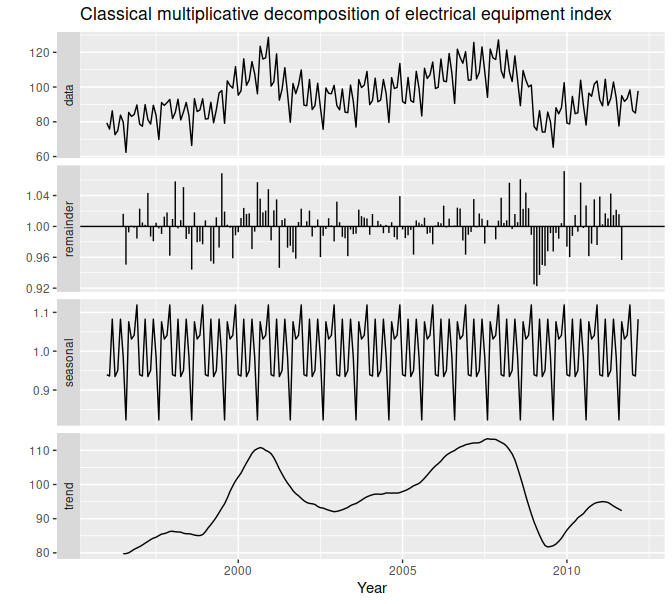
\includegraphics[width=.65\textwidth]{ej-descomposicion}
  \caption{Ejemplo de descomposición clásica de una serie.}
  \label{fig:ej-descomposicion}
\end{figure}

\subsubsection{Otras descomposiciones}

Existen otras descomposiciones que modifican el método que hemos descrito, entre ellas destacan la descomposición X11 \cite{shiskin1965x, dagum2016seasonal} o SEATS (\emph{Seasonal Extraction in ARIMA Time Series}) \cite{gomez1995programs, dagum2016seasonal}.

Una de las descomposiciones más famosas y la que usaremos en el proyecto será la descomposición STL (\emph{Sesonal and Trend decomposition using Loess}) \cite{cleveland1990stl}. Mostramos como ejemplo la descomposición de la serie que habíamos utilizado para la descomposición clásica \autoref{fig:stl-decomposition} (\cite{hyndman2018forecasting}).

\begin{figure}[htpb]
  \centering
  %\hspace*{-2.5cm}
  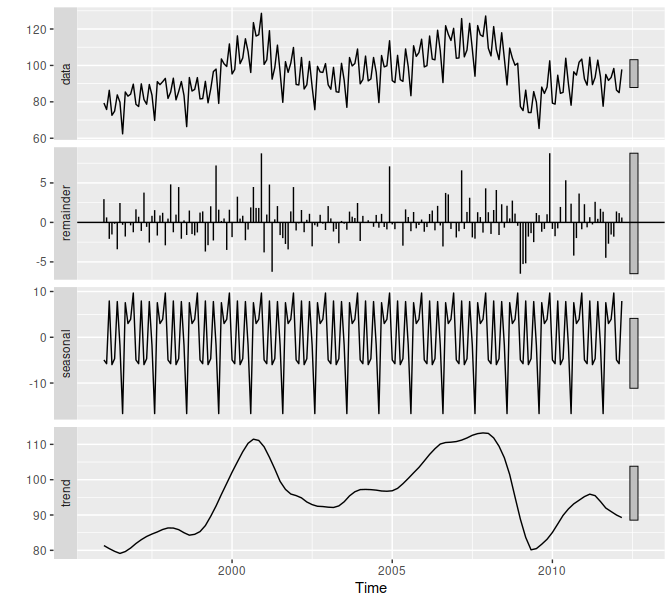
\includegraphics[width=.65\textwidth]{stl-decomposition}
  \caption{Ejemplo de descomposición STL de una serie.}
  \label{fig:stl-decomposition}
\end{figure}

\subsection{Predicción}

Una vez realizada la de composición de un proceso, nos planteamos como poder predecir valores futuros de la serie observada. Mostremos primero alguno de los predictores más simples.

\subsubsection{Predictores simples}

Empecemos primero por el \textbf{método de la media} (\emph{average method}), que considera la media de la serie (\autoref{def:metodo-medio}).

\begin{definicion}[Método de la media]
  Sea un proceso $\{X_t\}_{t = 1}^n$ del cual se toma una serie temporal $\{x_t\}_{t = 1}^n$, se define el método de la media como el predictor dado por

  $$\hat{x}_{n + \tau | n} = \hat{x} = \dfrac{1}{n}\sum \limits^n_{i = 1} x_i, $$

  donde $\hat{x}_{n + \tau | n}$ indica la estimación de $x_{n + \tau}$ en base a los datos $x_1, \ldots, x_n$.
  \label{def:metodo-medio}
\end{definicion}

El \textbf{método del camino aleatorio} (\emph{random walk method}) predice mediante el último valor de la observación (\autoref{def:metodo-ingenuo}).

\begin{definicion}[Método del camino aleatorio]
  Sea un proceso $\{X_t\}_{t = 1}^n$ del cual se toma una serie temporal $\{x_t\}_{t = 1}^n$, se define el método del camino aleatorio como el predictor dado por

  $$\hat{x}_{n + \tau | n} = x_n$$
  \label{def:metodo-ingenuo}
\end{definicion}

Para series con una alta estacionalidad funciona muy bien el \textbf{método de la ingenuidad estacional} (\emph{seasonal naîve method}) en el que se predice tomando la última observación que se corresponde con el periodo de la estacionalidad (\autoref{def:seasonal-naive}).

\begin{definicion}[Método de la ingenuidad estacional]
  Sea un proceso $\{X_t\}_{t = 1}^n$ del cual se toma una serie temporal $\{x_t\}_{t = 1}^n$, se define el método medio como el predictor dado por

  $$\hat{x}_{n + \tau | n} = x_{n + \tau - S(k + 1)},$$

  donde $S$ es el periodo de la componente estacional y $k$ la parte integral de $(\tau - 1)/S$.
  \label{def:seasonal-naive}
\end{definicion}

Finalmente el \textbf{método de deriva} (\emph{drift method}) que modifica el método del camino aleatorio añadiendo una tendencia derivada de la recta extrapolada entre el primer y último dato de la serie (\autoref{def:metodo-deriva}).

\begin{definicion}[Método de deriva]
  Sea un proceso $\{X_t\}_{t = 1}^n$ del cual se toma una serie temporal $\{x_t\}_{t = 1}^n$, se define el método medio como el predictor dado por

  $$\hat{x}_{n + \tau | n} = x_n + \tau \left(\dfrac{x_n - x_1}{n - 1}\right).$$
  \label{def:metodo-deriva}
\end{definicion}

Mostramos un ejemplo de funcionamiento de predicción de los métodos de la media (\emph{mean}, en rojo), del camino aleatorio (\emph{naïve}, en verde) e ingenuo estacional (\emph{seasonal naïve}, en azul) en \autoref{fig:ej-metodos1} (\cite{hyndman2018forecasting}).

\begin{figure}[htpb]
  \centering
  %\hspace*{-2.5cm}
  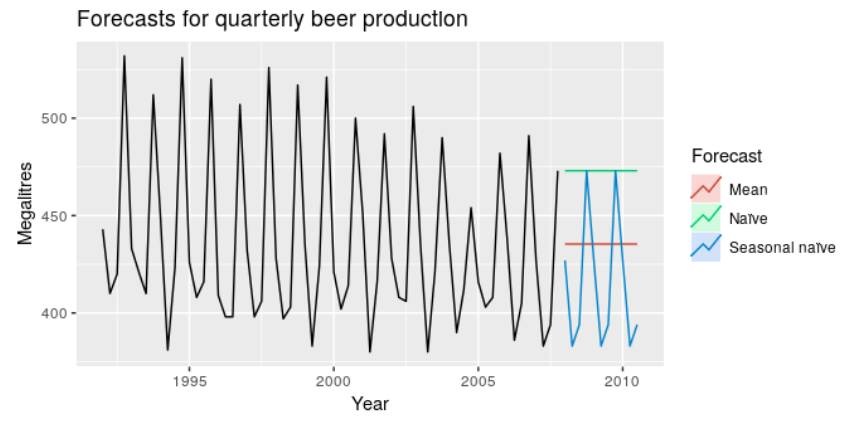
\includegraphics[width=.65\textwidth]{ej-metodos1}
  \caption{Ejemplo de predictores de la media, del camino aleatorio e ingenuo estacional.}
  \label{fig:ej-metodos1}
\end{figure}

Y otro con el método de deriva (\emph{drift}, en rojo), de la media (\emph{mean}, en verde) y del camino aleatorio (\emph{naïve}, en azul) en \autoref{fig:ej-metodos2} (\cite{hyndman2018forecasting}).

\begin{figure}[htpb]
  \centering
  %\hspace*{-2.5cm}
  \includegraphics[width=.65\textwidth]{ej-metodos2}
  \caption{Ejemplo de predictores de deriva, de la media y del camino aleatorio.}
  \label{fig:ej-metodos2}
\end{figure}

\subsubsection{Predictores con descomposición}

Cuando nos encontramos con un proceso general $\{X_t\}$ que parece presentar componentes estacionales y tendencia, realizamos una descomposición \eqref{eq:pred-decomp}

\begin{equation}
  X_t = m_t + s_t + Y_t, \; \forall t \in T,
  \label{eq:pred-decomp}
\end{equation}

de manera que hacemos las predicciones por separado para cada componente. Para la estacionalidad $s_t$, debido a su carácter periódico se puede utilizar el predictor ingenuo estacional, para la tendencia $m_t$ podemos predecir con el método de deriva o el método usado para el modelado de la tendencia (ajuste polinómico, suavizado) y finalmente para los residuos $Y_t$ que son estacionarios se puede modelar por ejemplo con un $ARMA$.

También es interesante considerar la descomposición \eqref{eq:decomp-nueva}

\begin{equation}
  X_t = s_t + a_t, \; \forall t \in T,
  \label{eq:decomp-nueva}
\end{equation}

donde $a_t = m_t + Y_t$ es la componente estacionalmente ajustada. En este caso se puede usar el predictor del camino aleatorio y también una modificación de $ARMA$ que veremos más adelante que utiliza otro enfoque para obtener una serie estacionaria.

Veamos un ejemplo de descomposición STL que predice utilizando el método ingenuo estacional para la estacionalidad y el método de camino aleatorio para la componente estacionalmente ajustada, junto con los intervalos de confianza \autoref{fig:stl-predict} (\cite{hyndman2018forecasting}).

\begin{figure}[htpb]
  \centering
  %\hspace*{-2.5cm}
  \includegraphics[width=.5\textwidth]{stl-prediccion}
  \caption{Ejemplo de predicción con descomposición STL y método ingenuo estacional y camino aleatorio con intervalos de confianza.}
  \label{fig:stl-predict}
\end{figure}

\section{Diferenciación}

Estudiamos el siguiente método para obtener un proceso estacionario de la serie observada, la \textbf{diferenciación}. Fundamentalmente consiste en aplicar diferencias entre observaciones contiguas de la serie para eliminar la tendencia y/o la estacionalidad, dejando un proceso estacionario.

\subsection{Procesos sin estacionalidad}

Primero veamos como aplicar el método de la diferenciación para procesos que no presentan una componente de estacionalidad, recordando el modelo definido en \autoref{def:solo-tendencia}.

Intentamos eliminar la tendencia usando la diferenciación. Introduzcamos antes  el operador de diferenciación con desfase 1 como \autoref{def:operador-diff}.

\begin{definicion}[Operador diferenciación $\nabla$]

Sea un proceso $\{X_t\}_{t \in T}$, se define el operador de diferenciación con desfase 1, notado como $\nabla$, aplicado al proceso $\{X_t\}$ como la siguiente expresión:

$$\nabla X_t = X_t - X_{t - 1} = (1 - B)X_t, \; \forall t \in T,$$

donde $B$ es el operador de desplazamiento hacia atrás definido por

$$BX_t = X_{t-1}, \; \forall t \in T.$$
\label{def:operador-diff}
\end{definicion}

Las potencias de los operadores se definen como uno podría esperar \eqref{eq:potencias-op}

\begin{gather}
  B^i(X_t) = X_{t-i}, \; \forall i \geq 1, \\
  \nabla^i(X_t) = \nabla(\nabla^{i-1}(X_t)), \; \forall i \geq 1, \\
  \nabla^0(X_t) = X_t.
\label{eq:potencias-op}
\end{gather}

Podemos manipular polinomios de $B$ y $\nabla$ de la misma manera que con polinomios de variables reales, por ejemplo \eqref{eq:diff-ej}

\begin{equation}
  \nabla^2X_t = \nabla(\nabla(X_t)) = (1-B)(1-B)X_t = (1 - 2B + B^2)X_t = X_t - 2X_{t-1} + X_{t-2}.
  \label{eq:diff-ej}
\end{equation}

Sea un proceso $\{X_t\}$ dado por \autoref{def:solo-tendencia} y supongamos que la tendencia es lineal, $m_t = c_0 + c_1t$. Aplicando la diferenciación a $\{X_t\}$ obtenemos \eqref{eq:diff-tendencia}

\begin{equation}
  \nabla X_t = \nabla m_t + \nabla Y_t = c_0 + c_1 t - c_0 - c_1(t - 1) + \nabla Y_t = c_1 + \nabla Y_t, \; \forall t \in T,
  \label{eq:diff-tendencia}
\end{equation}

queda una constante $c_1 \in \R$. Para ver que $\nabla X_t$ sea estacionario podemos ignorarla (la constante es la media), y ver si $\nabla Y_t$ es estacionario \eqref{eq:diff-estacionario}

\begin{equation}
  \begin{aligned}
  Cov[\nabla Y_t, \nabla Y_s] & = Cov[Y_t, Y_s] - Cov[Y_{t-1}, Y_s] - Cov[Y_t, Y_{s-1}] + Cov[Y_{t-1}, Y_{s-1}] \\
  & = \gamma_Y(t - s) - \gamma_Y(t - s - 1) - \gamma_Y(t - s + 1) + \gamma_Y(t - s) \\
  & = 2\gamma_Y(t - s) - \gamma_Y(t - s + 1) - \gamma_Y(t - s - 1), \; \forall t,s \in T,
  \end{aligned}
  \label{eq:diff-estacionario}
\end{equation}

al ser $Y_t$ estacionario. Como la covarianza no depende de $t$ y la media es constante ($c_1$) $\nabla X_t$ es estacionario. Para un ajuste polinómico general, $m_t = \sum \limits^n_{i = 0} c_i t^i$, e $Y_t$ estacionario tenemos que \eqref{eq:diff-general}

\begin{equation}
  \nabla^i X_t = i!c_i + \nabla^i Y_t, \; \forall t \in T,
  \label{eq:diff-general}
\end{equation}

un proceso estacionario con media $i!c_i$. Si la serie se puede ajustar relativamente bien con un polinomio de grado bajo, entonces al aplicar $\nabla$ unas cuantas veces obtendremos una serie estacionaria. En la práctica el orden de diferenciación necesario suele ser de 1 ó 2 nada más.

Un ejemplo lo tenemos aplicando $\nabla^2$ a la serie \autoref{fig:strikes} (\cite{brockwell2002introduction}) que produce la serie \autoref{fig:strikes-diff} \cite{brockwell2002introduction}, sin tendencias aparentes.

\begin{figure}[htpb]
  \centering
  %\hspace*{-2.5cm}
  \includegraphics[width=.35\textwidth]{strikes}
  \caption{Huelgas en EE.UU, 1951-1980.}
  \label{fig:strikes}
\end{figure}


\begin{figure}[htpb]
  \centering
  %\hspace*{-2.5cm}
  \includegraphics[width=.35\textwidth]{strikes-diff}
  \caption{Segundas diferencias ($\nabla^2$) en la serie de huelgas.}
  \label{fig:strikes-diff}
\end{figure}

\subsection{Procesos con estacionalidad}

Cuando el modelo contiene una componente estacional \autoref{def:descomposicion-entera} con un patrón que se repite cada cierto periodo $S$. Para lidiar con esto podemos extender el operador $\nabla$ que habíamos definido de desfase 1 a un $d$ genérico \autoref{def:diff-estacional}

\begin{definicion}[Operador diferenciación $\nabla_d$]
  Sea un proceso $\{X_t\}_{t \in T}$, el operador de diferenciación con desfase $d$, notado como $\nabla_d$, aplicado al proceso $\{X_t\}$ se define como

  $$\nabla_d X_t = X_t - X_{t - d} = (1 - B^d)X_t, \; \forall t \in T.$$
\label{def:diff-estacional}
\end{definicion}

Considerando un proceso $\{X_t\}$ dado como \autoref{def:descomposicion-entera}, donde el proceso estacional $\{s_t\}$ tiene periodo $S$, entonces podemos aplicar $\nabla_S$ obteniendo \eqref{eq:diff-estacional}

\begin{equation}
  \nabla_S X_t = m_t - m_{t - S} + Y_t - Y_{t - S}, \; \forall t \in T,
\label{eq:diff-estacional}
\end{equation}

mostrando que el proceso $\nabla_S X_t$ no tiene estacionalidad, por lo que se le pueden aplicar los métodos conocidos para los métodos no estacionales. En particular ahora se le puede aplicar una potencia del operador $\nabla$.

Un ejemplo de modelo donde hemos aplicado $\nabla_12 \nabla$ lo tenemos en \autoref{fig:diff-season} (\cite{hyndman2018forecasting}) que se ha aplicado primero una transformación logarítmica, una transformación común para series que aumentan o decrecen con el tiempo (es equivalente a usar un modelo multiplicativo).

\begin{figure}[htpb]
  \centering
  %\hspace*{-2.5cm}
  \includegraphics[width=.5\textwidth]{diff-season}
  \caption{Generación de electricidad mensual en EEUU, con transformación logarítmica, diferenciación estacional ($\nabla_{12}$) y una diferenciación ($\nabla$) (de arriba a abajo, respectivamente).}
  \label{fig:diff-season}
\end{figure}

La transformación logarítmica estabiliza las variaciones de la serie, y la diferenciación estacional quita la componente estacional completamente. La diferenciación adicional deja la serie como un proceso estacionario.

\subsection{Modelo ARIMA}

Existe una modificación de los modelos ARMA para considerar directamente el modelado con series sin estacionalidad: el modelo \textbf{ARIMA} (modelos autorregresivos integrados de media móvil) \cite{box2011time}. Juntaremos el modelo ARMA con la idea de realizar una diferenciación $\nabla^d$ para modelar directamente cualquier serie sin estacionalidad \autoref{def:arima}.

\begin{definicion}[Modelo ARIMA]
  Un proceso $\{X_t\}_{t \in T}$ se dice que es un proceso $ARIMA(p, d, q)$ si el proceso definido por

  $$ Y_t = (1 - B)^d X_t, \; \forall t \in T,$$

  es un proceso $ARMA(p, q)$.
\label{def:arima}
\end{definicion}

Mostramos ejemplos $ARIMA$ simulados con sus correlogramas: $ARIMA(1, 1, 1)$ dado por $(1 + \frac{1}{2}B)(1-B)X_t = (1+\frac{3}{10}B)Z_t$ y $ARIMA(1, 1, 2)$ dado por $(1 - \frac{3}{5}B)(1-B)X_t = (1-\frac{3}{10}B+\frac{1}{2}B^2)Z_t$ \autoref{fig:ej-arima} (\cite{chatfield2019analysis}).

\begin{figure}[htpb]
  \centering
  %\hspace*{-2.5cm}
  \includegraphics[width=.7\textwidth]{ej-arima}
  \caption{Modelos simulados $ARIMA(1, 1, 1)$ (arriba) y $ARIMA(1, 1, 2)$ (abajo).}
  \label{fig:ej-arima}
\end{figure}

\subsection{Modelo SARIMA}

Si incluimos la diferenciación estacional $\nabla_S$ al modelo ARIMA podremos extender los modelos ARMA para series que manifiestan una componente estacional, este es el modelo \textbf{SARIMA} (Seasonal ARIMA) \autoref{def:sarima} (\cite{box2011time}).

\begin{definicion}[Modelo SARIMA]
  Un proceso $\{X_t\}_{t \in T}$ se dice que es un modelo $SARIMA(p,d,q)\times(P,D,Q)_S$ con periodo $S$ si la serie diferenciada $Y_t = (1 - B)^d(1 - B^S)^D X_t$ es un proceso ARMA definido por

  $$\phi(B)\Phi(B^S)Y_t = \theta(B)\Theta(B^S)Z_t, \; \forall \tau \in T,$$

  donde $\{Z_t\}_{t \in T} \sim WN(0, \sigma^2)$, $\phi(z) = 1 - \phi_1 z - \cdots - \phi_p z^p$, $\Phi(z) = 1 - \Phi_1z - \cdots - \Phi_P z^P$, $\theta(z) = 1 + \theta_1 z + \cdots + \theta_qz^q$ y $\Theta(z) = 1 + \Theta_1z + \cdots + \Theta_Q z^Q$.
\label{def:sarima}
\end{definicion}

Un ejemplo de modelo $SARIMA(3, 0, 1)(0, 1, 2)_12$ predictor en una serie lo tenemos en \autoref{fig:ej-sarima} (\cite{hyndman2018forecasting}) junto a los intervalos de confianza.

\begin{figure}[htpb]
  \centering
  %\hspace*{-2.5cm}
  \includegraphics[width=.6\textwidth]{ej-sarima}
  \caption{Predicciones del modelo $SARIMA(3, 0, 1)(0, 1, 2)_12$.}
  \label{fig:ej-sarima}
\end{figure}


\endinput

% !TeX root = ../libro.tex
% !TeX encoding = utf8
%
%*******************************************************
% Métricas
%*******************************************************

\chapter{Métricas}\label{ch:metricas}

Enumeramos y explicamos distintas \textbf{métricas}: funciones que nos sirven para medir la bondad del ajuste de los modelos en distintos problemas. Es importante no confundir la métrica usada para medir el rendimiento de los modelos, con la función de error o pérdida que usa cada modelo concreto y trata de minimizar, ya que se puede minimizar distintas funciones de error pero que impliquen un buen resultado en la métrica; aun así es posible que coincida la métrica con la función de error.

Según la tipología del problema podemos encontrar distintas métricas donde veremos las más importantes de los problemas de clasificación y regresión.

\section{Clasificación}

En los problemas de clasificación nos encontramos con aprendizaje \textbf{supervisado} ya que generalmente tenemos unas etiquetas asociados a los datos que queremos predecir correctamente. Según el modelo puede tener dos tipos de enfoque para los que tendremos distintos tipos de métricas: predicción de etiquetas (clasificador "duro") o predicción de probabilidades asociadas a las clases (clasificador "flexible").

Planteamos antes el problema general de clasificación con $n$ clases (\autoref{def:clasgen}).

\begin{definicion}[Problema de clasificación multiclase]
  Sea $M \in \N$ la longitud de las series, $N \in \N$ el número de series y $n$ el número de clases, se considera el espacio $\mathcal{X} \times Y \subseteq \R^M \times \{0, 1, \ldots, n - 1\}$ del que se extrae una muestra $(X, \textbf{y}) \in \mathcal{X}^N \times Y^N$ que sigue una distribución $\mathcal{P}$ desconocida y el espacio de funciones del modelo dado $\mathcal{H}$.

  El problema consiste en encontrar un $h \in \mathcal{H}$ de tal manera que $h \approx f$, siendo $f$ la función de etiquetado:

  \begin{align*}
    f : \mathcal{X} & \to Y \\
    \textbf{x} & \mapsto f(\textbf{x}) \in \{0, 1, 2, \ldots, n - 1\}
  \end{align*}
  \label{def:clasgen}
\end{definicion}

Como nota, en los problemas de clasificación binarios se suele indicar una clase como la positiva ($+1$) y la otra como la negativa ($-1$); normalmente la positiva es la que tiene más relevancia para ser detectada que la negativa, aunque no tiene por qué. Ademas, en clasificación multiclase se puede considerar la clase más importante, si la hubiera, como la positiva y el resto la negativa; o también considerar para cada clase como si fuese la positiva y tomar la media de todos los resultados.

\subsection{Etiquetas}

Si nuestro clasificador devuelve etiquetas, suponiendo que la muestra tiene las clases balanceadas y que importan lo mismo, la métrica más usada es el acierto (\emph{accuracy}) que mide simplemente la proporción de correspondencia de las etiquetas predichas con las originales.

Sea la función aprendida por un modelo $h \in \mathcal{H}$, definimos $acc$ como \refeq{eq:acc}. Considerando que $acc \in [0, 1]$ se puede también usar la función de pérdida asociada como \refeq{eq:acc_loss}, aunque es más frecuente usar $acc$.

\begin{equation}
  acc(h) = \frac{1}{n} \sum \limits^N_{i = 1}[[h(\textbf{x}_i) = y_i]]
  \label{eq:acc}
\end{equation}

\begin{equation}
  E(h) = 1 - acc(h)
  \label{eq:acc_loss}
\end{equation}

Cuando la clase positiva importa más que la negativa tenemos que medir de otra manera que sea influya más una clase que la otra. Para ello introducimos los los conceptos de \textbf{precisión} ($precision$) y \textbf{sensibilidad} ($recall$):

\begin{enumerate}
  \item \textbf{Precisión}: definido en \eqref{eq:precision}, evalúa la proporción de las clases positivas correctamente clasificadas frente a todas las etiquetas como la clase positiva. Si el modelo es muy preciso nos indica que cuando el modelo etiqueta un dato con la clase positiva casi seguro que lo sea.
  \item \textbf{Sensibilidad}: definido en \eqref{eq:recall}, evalúa la proporción de las clases positivas correctamente clasificadas frente a todas las clases positivas que hay, bien o mal clasificadas. Si el modelo es muy sensibile nos indica que clasifica correctamente la mayoría de datos con etiqueta positiva.
\end{enumerate}

\begin{equation}
  precision = \dfrac{verdaderos\_positivos}{verdaderos\_positivos + falsos\_positivos}
  \label{eq:precision}
\end{equation}

\begin{equation}
  recall = \dfrac{verdaderos\_positivos}{verdaderos\_positivos + falsos\_negativos}
  \label{eq:recall}
\end{equation}

Usando estos dos valores se obtiene la métrica $F_\beta$ \eqref{eq:fscore}, donde variamos el $\beta$ usado según la matriz de costes asociados a los falsos positivos y negativos. Generalmente se usa $F_1$ cuando cuestan igual, $F_{0.5}$ si los falsos positivos cuestan mas y $F_{2}$ si son los falsos negativos.

\begin{equation}
  F_\beta = (1 + \beta^2) \cdot \dfrac{precision \cdot recall}{(\beta^2 \cdot precision) + recall}
  \label{eq:fscore}
\end{equation}

\subsection{Probabilidades}

Aunque el clasificador devuelve probabilidades generalmente necesitamos dar una respuesta con etiquetas, por lo que se suele dar un \textbf{umbral} para el que clasificar de una clase (problema binario) o tomar la clase con mayor probabilidad si se están prediciendo probabilidades para todas las clases.

En cualquier caso las dos métricas mas usadas generalmente son las que miden el \textbf{área bajo la curva} de las funciones \textbf{precision-recall} ($PR-AUC$) y \textbf{Receiver Operating Characteristic} ($ROC-AUC$). En ambos casos se crea una curva en el cuadradado $[0,1] \times [0,1]$ donde se integra para obtener el área que deja la curva, haciendo que ambas métricas tomen valores en $[0, 1]$ siendo mejor el modelo cuanto más alto valga.

Cuando la clase positiva importa igual que la clase negativa se toma $ROC-AUC$ que mide el comportamiento del modelo obteniendo las tasas de falsos positivos ($falsos\_positivos$) y verdaderos positivos ($verdaderos\_positivos$) para cada umbral de probabilidad que se va poniendo al modelo. Se suele imprimir el gráfico con la curva que forma comparando con el clasificador aleatorio para compararlo (\autoref{fig:ej-roc} \cite{scikit2020roc}).

\begin{figure}[htpb]
  \centering
  %\hspace*{-2.5cm}
  \includegraphics[width=.6\textwidth]{ej-roc}
  \caption{Ejemplo de curva ROC.}
  \label{fig:ej-roc}
\end{figure}

Por otro lado, si la clase positiva tiene mayor importancia entonces se coge $PR-AUC$ que en este caso mide la precisión y la sensibilidad del modelo frente a distintos umbrales de probabilidad. También se incluye un modelo aleatorio para hacer la comparación, donde encontramos un ejemplo en \autoref{fig:ej-pr} \cite{scikit2020pr}.

\begin{figure}[htpb]
  \centering
  %\hspace*{-2.5cm}
  \includegraphics[width=.6\textwidth]{ej-pr}
  \caption{Ejemplo de curva PR.}
  \label{fig:ej-pr}
\end{figure}

\section{Regresión}

Un problema de regresión no es más que un problema de clasificación donde las etiquetas no son discretas si no continuas (\autoref{def:probregresion}).

\begin{definicion}[Problema de regresión]
  Sea $M \in \N$ la longitud de las series y $N \in \N$ el número de series y $n$ la dimensión de las etiquetas, se considera el espacio $\mathcal{X} \times \mathcal{Y} \subseteq \R^M \times \R^n$ del que se extrae una muestra $(X, Y) \in \mathcal{X}^N \times \mathcal{Y}^N$ que sigue una distribución $\mathcal{P}$ desconocida y el espacio de funciones del modelo dado $\mathcal{H}$.

  El problema consiste en encontrar un $h \in \mathcal{H}$ de tal manera que $h \approx f$, siendo $f$ la función de etiquetado:

  \begin{align*}
    f : \mathcal{X} & \to \mathcal{Y} \\
    \textbf{x} & \mapsto f(\textbf{x}) \in \R^n
  \end{align*}
  \label{def:probregresion}
\end{definicion}

Generalmente se usan las siguientes métricas principales, donde todas toman valores en $[0, +\infty)$ siendo cuanto más bajo mejor:

\begin{enumerate}
  \item \textbf{Error Medio Absoluto} (\emph{Mean Absolute Error}, MAE): definido en \eqref{eq:mae}, se suele usar para no tener en cuenta el efecto de los valores atípicos ya que es menos sensible a estos.
  \item \textbf{Error Cuadrático Medio} (\emph{Mean Squared Error}, MSE): definido en \eqref{eq:mse}, es una de las métricas mayormente usadas y añade importancia a errores grandes, ya que se aplica un cuadrado.
  \item \textbf{Raíz del Error Cuadrático Medio} (\emph{Root Mean Squared Error}, RMSE): definido en \eqref{eq:rmse}, hace que las medidas del MSE vuelvan a la unidad, dando una mejor interpretabilidad.
\end{enumerate}

\begin{equation}
  MAE(h) = \dfrac{1}{n} \sum \limits^N_{i = 1} || \textbf{y}_i - h(\textbf{x}_i) ||_1
  \label{eq:mae}
\end{equation}

\begin{equation}
  MSE(h) = \dfrac{1}{n} \sum \limits^N_{i = 1} || \textbf{y}_i - h(\textbf{x}_i)) ||^2_2
  \label{eq:mse}
\end{equation}

\begin{equation}
  RMSE(h) = \sqrt{MSE(h)}
  \label{eq:rmse}
\end{equation}

\endinput


% --------------------------------------------------------------------
% MAINMATTER
% --------------------------------------------------------------------
%\mainmatter % activa la numeración de capítulos, resetea la numeración de las páginas y usa números arábigos

\setpartpreamble[c][0.75\linewidth]{
	\bigskip % Deja un espacio vertical en la parte superior
  Estudiamos una nueva heurística alternativa a la selección clásica de modelos: \emph{Perturbation Validation} ($PV$).
  Este método intenta medir si la función aprendida por un modelo se ajusta correctamente a la función que se está intentando aprender, intentando ser un \textbf{método complementario} a la selección en base a la validación clásica de usar particiones entrenamiento/test junto a la validación cruzada. Este método nuevo es bastante útil para la \textbf{búsqueda de hiperparámetros} del modelo, donde la validación clásica a veces no es capaz de discernir entre varios modelos con un rendimiento parecido, pero que alguno puede estar sobreajustando mucho más los datos.

  En \autoref{ch:pv-introduccion} se introduce el contexto bajo el que surge el $PV$ y que se va a intentar obtener, definiéndolo formalmente y describiendo su implementación en \autoref{ch:pv}. Finalmente realizamos los experimentos para comprobar su utilidad, junto con los resultados y las conclusiones en \autoref{ch:pv-experimentacion}.
}
\part{Selección de modelos}\label{part:pv}
  % !TeX root = ../libro.tex
% !TeX encoding = utf8

\chapter{Introducción}\label{ch:pv-introduccion}

La \textbf{selección de modelos} es una tarea muy importante en la resolución de problemas del aprendizaje automático (y profundo) ya que de entre varios modelos propuestos como solución querremos escoger el mejor.

Para valorar esto recurrimos a las \textbf{métricas}, aplicaciones que miden cuantitativamente, usando algún criterio, la semejanza entre la función $f$ que estamos intentando aprender y la función $h$ aprendida por el modelo.

Usando una métrica podemos comparar los resultados entre distintos modelos y escoger el que mayor valor arroje, sin embargo aquí entra el problema de la \textbf{validación}. Si solo nos basamos con el resultado de la métrica en el mismo conjunto donde hemos entrenado los datos, puede que estemos sobrestimando bastante el valor real debido al efecto del \textbf{sobreajuste}.

Recordemos que este efecto se daba cuando el modelo se ajustaba demasiado a los datos de la muestra actual obteniendo un sesgo muy bajo, sin embargo, vimos que también la varianza aumentaba mucho, provocando que para otra muestra distinta de la distribución el modelo obtuviese un rendimiento mucho peor al de la muestra donde fue entrenada.

Por esta razón es necesaria una manera más realista de medir los modelos para evitar el sobreajuste, surgiendo así la \textbf{división clásica} entrenamiento/test. Este método consiste en, o bien obtener dos muestras independientes de la distribución o dividir una única muestra en dos antes de manipular los datos. La muestra de entrenamiento se usa para entrenar el modelo y la muestra de test para valorar los modelos, ya que es una nueva muestra que no ha visto el modelo anteriormente.

Aunque este método ya resuelva nuestro problema también se puede querer hacer la selección de los modelos antes de realizar la valoración en el conjunto de test para, por ejemplo, quedarnos con un subconjunto menor de modelos de un gran número de modelos considerados para reducir tiempo de cómputo innecesario. También entra aquí la \textbf{selección de hiperparámetros} que es una selección de modelos solo que considerando el mismo modelo base y lo que cambia entre modelos es algún hiperparámetro (por ejemplo el número de neuronas en una red neuronal).

Para resolver esto hay generalmente dos alternativas: hacer una partición más del conjunto de entrenamiento, quedándonos en total con el de entrenamiento, test y el de \textbf{validación}; o bien utilizar el método de \textbf{validación cruzada}.

La validación cruzada consiste en dividir la muestra de entrenamiento en $k$ conjuntos del mismo tamaño y repetir $k$ veces la validación usando un conjunto como \emph{test} y el resto de entrenamiento. Este método intenta dar un valor más robusto que usando un único conjunto de validación, y además puede indicar una idea de cómo de variable será en función a la varianza de los resultados.

Estos son los métodos clásicos que se han usado generalmente para obtener valores de la métrica realistas y que nos permiten comparar modelos y por tanto, elegir los mejores en base a esto. Sin embargo, esta clase de validaciones confía que en las muestras de datos recogidas de la distribución es \textbf{suficientemente representativa} de la distribución subyacente, y que han sido recogidos \textbf{sin sesgo} alguno \cite{zhang2019perturbation}.

Estos problemas se puede presentar perfectamente cuando el problema es muy grande y es muy difícil obtener muchas muestras, o cuando se ha cometido algún error al tomar las muestras que nadie se ha percatado. Por ejemplo, en la detección de caras en imágenes, debido a la gran cantidad de posibilidades de formas en las que podrían estar, se necesita una muestra muy grande que abarque múltiples y diversas maneras para poder tener una representación buena de la distribución y además que no haya sesgos (solo salen caras en fotos con buena iluminación, o de gente con tez blanca...).

Por estas razones se presenta un nuevo método para valorar modelos basado en una heurística: $PV$ (\emph{Perturbated Validation}) \cite{zhang2019perturbation}. Este método \textbf{no} utiliza las mismas técnicas clásicas de utilizar un conjunto aparte sino que considera todo el conjunto entero, sin divisiones. En lineas generales trata de valorar si el modelo ha entendido realmente \textbf{la relación subyacente de los datos} midiendo como varía el comportamiento del modelo frente a \textbf{perturbaciones graduales} en los datos.

Nuestro objetivo será ver el funcionamiento de esta heurística, su comportamiento en casos reales, mediante una experimentación utilizando muchos modelos y conjuntos de datos para observar y analizar si nos resulta de utilidad y puede aportar algo nuevo en el paradigma actual de selección de modelos.

\chapter{Selección de modelos}\label{ch:pv}

Planteamos el problema de la selección de modelos para problemas de clasificación multiclase en dominios de series temporales: sea $M \in \N$ la longitud de cada serie temporal, $N$ el número de series temporales, $n$ el número de clases y $k$ el número de modelos a ajustar, consideramos el espacio $\mathcal{X} \times Y \subseteq R^m \times \{0, 1, \ldots, n - 1\} $ del que se obtiene una muestra $(X, \textbf{y}) \in \mathcal{X}^N \times Y^N$ (datos $X$ y etiquetas $\textbf{y}$) que sigue una distribución de probabilidad $\mathcal{P}$ desconocida. Sean también el espacio de hipótesis de los modelos considerados $\mathcal{H} = \{\mathcal{H}_1, \ldots, \mathcal{H}_k\}$ de los que se ha obtenido una función cada uno $h_i \in \mathcal{H}_i, \, i = 1, \ldots, k$ que intentan aproximar a la función de etiquetado $f$ definida por:

\begin{align*}
  f : \mathcal{X} & \to Y \\
  \textbf{x} & \mapsto f(\textbf{x}) \in \{0, 1, \ldots, n-1\}.
\end{align*}

Se pide valorar bajo un criterio determinado la aproximación de las funciones de hipótesis a la función de etiquetado (valorar $f \approx h_i$) de manera que se establezca un orden entre los modelos, permitiéndonos seleccionar los modelos con mejor valoración bajo este criterio.

\section{Selección clásica}

Consideramos la selección de modelos clásica: primero tomamos la muestra o \emph{dataset} $(X, \textbf{y})$ de la realizamos una partición en un conjunto de entrenamiento (\emph{train}) y test usando la proporción usual de 80/20\% respectivamente, manteniendo la proporción de clases. Después realizaremos el método de Validación Cruzada con $k$ \emph{pliegues} (\emph{Cross Validation with $k$ folds}, $k$-CV) \cite{stone1974cross} en el conjunto de entrenamiento: como explicamos previamente, consiste en dividir el conjunto de entrenamiento en $k$ subconjuntos de tamaño igual que mantienen la proporción de clases y repetir $k$ veces la validación usando un subconjunto como test y el resto como entrenamiento (\autoref{fig:cv}, \cite{niu2018rfamyloid}).

\begin{figure}[htbp]
  \centering
  %\hspace*{-2.5cm}
  \includegraphics[width=.8\textwidth]{cv}
  \caption{Funcionamiento de la validación cruzada.}
  \label{fig:cv}
\end{figure}


La validación en este caso consiste en entrenar el modelo en el subconjunto de entrenamiento y obtener el valor de la métrica en el subconjunto test; una vez se obtienen los $k$ valores de la métrica se toma el valor final como la media de los valores aunque también se suele devolver la desviación típica o la varianza para tener una idea de cómo puede variar este valor (en qué intervalo de confianza se mueve la métrica).

Para problemas de clasificación consideraremos la métrica \emph{accuracy} $acc$ que ya vimos en \autoref{ch:metricas} que básicamente mide el porcentaje de etiquetas predichas correctamente. Utilizando esta métrica junto a la validación cruzada para cada modelo se obtendrá $acc_{CV}$, y en base a este valor podremos hacer la selección de modelos tomando en cuenta que es un estimador de la métrica en el conjunto test $acc_{test}$; por tanto lo esperable es que el mejor $acc_{CV}$ será probablemente el mejor $acc_{test}$.

\section{Perturbated Validation}

\subsection{Funcionamiento}

La idea general del $PV$ es ir midiendo la métrica $acc$ del modelo conforme se van añadiendo perturbaciones graduales en función de una ratio de error $r$ en la muestra de datos, tomando el valor del $PV$ como el valor absoluto de la \textbf{pendiente} de la recta de regresión con los puntos formados por las tasas de acierto y error $(acc, r)$.

En otras palabras, crearemos $n$ conjuntos copiando las etiquetas originales y cada conjunto con un $r$\% de etiquetas cambiadas. El modelo se entrena por separado con cada conjunto de etiquetas perturbadas y evaluando la métrica en el mismo conjunto, obteniendo así $n$ valores del $acc$ distintos. Es importante entender que el modelo no se reentrena, es como si copiásemos $n$ veces el modelo y cada uno se entrenase y evaluase en un conjunto distinto \textbf{independientemente}.

Teniendo ahora $n$ puntos $\{(r_1, acc_1), \ldots, (r_n, acc_n)\}$ ordenados por $r_1 < \ldots < r_n$ que podemos representar en $\R^2$, usamos regresión lineal para intentar ajustar una recta a los puntos lo mejor posible. El $PV$ entonces será simplemente el valor absoluto de la pendiente de esta recta.

Si el modelo es bueno y capta bien la relación de los datos con las etiquetas entonces no debería ser \emph{engañado} por las etiquetas mal puestas. Esto implica que cuando las etiquetas están casi sin alterar el modelo obtiene un $acc$ muy alto, pero conforme aumentan las perturbaciones el $acc$ va bajando. Entonces al hacer la regresión lineal obtendremos una recta con una pendiente muy pronunciada que se traduce en un $PV$ alto.

Si por el contrario el modelo es muy complejo y se ajusta demasiado a los datos, provocando \textbf{sobreajuste}, entonces obtendrá valores de $acc$ muy altos en todos los casos. La recta de regresión obtenida será muy horizontal y por tanto, con un $PV$ casi nulo. Finalmente, si la complejidad del modelo es insuficiente para captar los datos obtendrá $acc$ muy bajos, variando muy poco y obteniendo una recta horizontal también (\autoref{fig:ej-pv} \cite{zhang2019perturbation}).

\begin{figure}[htpb]
  \centering
  %\hspace*{-2.5cm}
  %\vspace*{-1.5cm}
  \includegraphics[width=0.6\textwidth]{ej_pv}
  \caption{Idea general de funcionamiento del $PV$.}
  \label{fig:ej-pv}
\end{figure}

Así, el $PV$ intenta medir la correspondencia entre la función de etiquetado real con la aprendida a partir del modelo y del que se esperan dos consecuencias:

\begin{itemize}
  \item Para un valor muy alto la función aprendida $h$ debe ser muy parecida a $f$ y por tanto debería tener valores muy altos de $acc$ en cualquier conjunto.
  \item Para un valor muy bajo la función no se parece, donde pueden pasar dos cosas:
    \begin{itemize}
      \item Si $acc_{train}$ es bajo, entonces es que el modelo tiene un ajuste directamente malo y en $acc_{test}$ también lo será.
      \item Si $acc_{train}$ es alto, entonces el modelo probablemente ha sobreajustado los datos y se tenga que $acc_{test}$ sea mucho menor y haya una gran diferencia con $acc_{train}$.
    \end{itemize}
\end{itemize}

Sin embargo, puede haber casos en los que tengamos un $PV$ bajo y obtengamos $acc_{test}$ bastantes altos, esto es consecuencia de cómo sean las muestras obtenidas de la distribución desconocida, si tienen alguno de los problemas que hemos mencionado (sesgo o representatividad insuficiente) entonces no se verá reflejado el problema en el conjunto de test y los modelos funcionarán igual de bien.

Veamos esto con un ejemplo de \cite{zhang2019perturbation} \autoref{fig:pv-decision} donde se han creado tres \emph{datasets} sintéticos con unas funciones de etiquetado bien definidas, en forma de lunas, círculos y lineal, y se han entrenando con distintos modelos obteniendo tres valores de las métricas utilizadas, PV ($PV$), CV ($acc_{CV}$) y TA ($acc_{test}$) junto con la funciones aprendidas de cada modelo (se corresponde el valor de la etiqueta con un color).

\begin{figure}[htpb]
  \centering
  \hspace*{-1.cm}
  \includegraphics[width=1.2\textwidth]{pv_decision}
  \caption{Tres funciones distintas de clasificación con varios modelos, recogiendo $PV$, $acc_{CV}$ y $acc_{test}$ y la función aprendida.}
  \label{fig:pv-decision}
\end{figure}

Observando los valores PV vemos cómo son mucho más altos cuando la función aprendida del modelo se corresponde con la \emph{forma} original de la función y esto se corresponde con valores casi perfectos de CV y TA. Por otro lado, se asignan valores bajos de PV para los modelos con funciones con una forma más complicada (Random Forest por ejemplo) o cuando no es capaz de captar bien la relación de los datos (Linear SVM), aunque en el primer caso se sigue teniendo valores casi perfectos de CV y TA reflejando lo que habíamos comentado previamente.

Desde luego entre varios modelos con valores CV en torno a 1 podríamos hacer otra selección con quien tenga un mayor valor de PV ya que preferimos quedarnos con un modelo que lo hace igual de bien que el resto pero la función que ha aprendido se adapta mucho más a la \textbf{distribución real de los datos}.

\subsection{Definición}

Sea $r \in [0, 1]$ el ratio de etiquetas perturbadas para cada clase (para mantener las distribución), consideramos una sucesión creciente de ratios $\{r_i\}_{1 \leq i \leq n}$ e $\textbf{y}_{r_i}$ el conjunto de etiquetas con un $r_i$ porcentaje de etiquetas perturbadas por clase. Finalmente notamos $acc(S)$ como el máximo valor de la métrica obtenido con $\mathcal{H}$ en $S = (X, \textbf{y}_{r_i})$, es decir \eqref{eq:acc_rel} \cite{zhang2019perturbation}.

\begin{equation}
  acc(S) = \max_{h \in \mathcal{H}} acc(h) \text{, con } S = (X, \textbf{y}_{r_i}).
  \label{eq:acc_rel}
\end{equation}

Con todos estos elementos ya podemos definir formalmente la heurística $PV$ (\autoref{def:pv}, \cite{zhang2019perturbation}).

\begin{definicion}[Perturbated Validation]\label{def:pv}
  $PV$ es el valor absoluto del coeficiente de la regresión lineal (la pendiente) entre la variable independiente, ratio de etiquetas perturbadas $r_i$, frente la variable dependiente, acierto en el \emph{dataset} perturbado $acc(S_{r_i})$, es decir,

  $$PV = \Bigg|\dfrac{\sum \limits^n_{i = 0} (r_i - \overline{r})(acc(S_{r_{i}}) - \overline{acc(S_r)})}{\sum \limits^n_{i = 0}(r_i - \overline{r})^2}\Bigg|.$$
\end{definicion}

\subsection{Implementación}

Se ha implementado en una clase en \emph{Python} denominada \textbf{$PV$} que nos permite evaluar los modelos usando la descripción mencionada anteriormente. La documentación se puede encontrar en \autoref{ap:documentacion}, aunque merece la pena describir el algoritmo general con pseudocódigo: \autoref{alg:create_pv} para crear los conjuntos de etiquetas perturbados y \autoref{alg:calc_pv} para calcular el $PV$ para un modelo dado.

\begin{algorithm}[htbp]
\SetAlgoLined
 \tcp{Inicializamos los ratios de error}
 \For{$i = 1, \ldots, n$}{
   $r_i \gets err_{ini} + (i - 1) \cdot \dfrac{err_{fin} - err_{ini}}{n - 1}$\;
 }
 \tcp{Para cada ratio creamos unas etiquetas perturbadas}
 \For{$i = 1, \ldots, n$}{
   \tcp{Copiamos las etiquetas originales}
   $\textbf{y}^{(i)} \gets \textbf{y}$\;
   \tcp{Perturbamos para cada clase}
   \For{$j = 1, \ldots, n_{clases}$}{
    \tcp{Perturbamos el \% respecto el número de etiquetas de esa clase}
    $n_{per} \gets r_i \cdot \sum \limits^{|\textbf{y}|}_{k = 1} [[y_k = j]]$\;
    \tcp{Hacemos una permutación de los índices de la clase para escogerlos aleatoriamente}
    $\sigma \gets Permutacion\left( \{ i \in \N : y_i = j\}\right)$\;
    \tcp{Para cada índice se le pone una clase aleatoria distinta de la original}
    \For{$k = 1, \ldots, n_{per}$}{
     $\textbf{y}^{(i)}_{\sigma(k)} \gets Aleatorio(\{1, 2, \ldots, j - 1, j + 1, \ldots, n_{clases}\})$\;
    }
   }
 }
 \KwResult{$r_1, \ldots, r_n$, $\textbf{y}^{(1)}, \ldots, \textbf{y}^{(n)}$}
 \caption{$PV$($\textbf{y}$, $n$, $err_{ini}$, $err_{fin}$)}
 \label{alg:create_pv}
\end{algorithm}

\begin{algorithm}[htbp]
\SetAlgoLined
 \tcp{Para cada conjunto entrenamos el modelo y obtenemos el \emph{accuracy}}
 \For{$i = 1, \ldots, n$}{
  $modelo_{copia} \gets $ copiar($modelo$)\;
  $modelo_{copia}$.fit($X$, $\textbf{y}^{(i)}$)\;
  $acc_i \gets modelo_{copia}$.score($X$, $\textbf{y}^{(i)}$)\;
 }
 \tcp{Calculamos las medias de los errores y el \emph{accuracy}}
 $\overline{r} \gets \dfrac{1}{n} \sum \limits_{i = 1}^{n} r_i$\;
 $\overline{acc} \gets \dfrac{1}{n} \sum \limits_{i = 1}^{n} acc_i$\;
 \tcp{Calculamos el $PV$}
 $PV \gets \Bigg|\dfrac{\sum \limits^n_{i = 0} (r_i - \overline{r})(acc_i - \overline{acc})}{\sum \limits^n_{i = 0}(r_i - \overline{r})^2}\Bigg|$\;
 \KwResult{$PV$}
 \caption{Calcular-$PV$($modelo$, $X$, $\textbf{y}^{(1)}, \ldots, \textbf{y}^{(n)}$, $r_1, \ldots, r_n$)}
 \label{alg:calc_pv}
\end{algorithm}

Para crear los \emph{datasets} perturbados tomamos los errores de manera que sean \textbf{equidistantes}, por lo que solo hace falta pasar como argumento el número de perturbaciones deseadas $n$, y los errores de inicio y fin $err_{1}$ y $err_{n}$. A la hora de elegir los índices aleatoriamente se toman de manera que todos sean \textbf{diferentes} y de la clase correspondiente en el bucle. La clase que se escoge también se asegura que no sea la que tiene actualmente, de manera que la serie tenga efectivamente una \textbf{etiqueta distinta} asociada. Devolvemos las etiquetas perturbadas $Y_i$ como los índices de error $r_i$ necesarios para calcular el $PV$.

Para obtener el $PV$ introducimos el modelo con el resultado del algoritmo anterior, obteniendo un $acc_i$ asociado con cada entrenamiento y medición de rendimiento del modelo (notar que se copia el modelo para que se entrene desde cero). Finalmente obtenemos el $PV$ para el modelo pasado.

\chapter{Experimentación}\label{ch:pv-experimentacion}

En este capítulo vamos a realizar un experimento empírico para investigar la eficacia del $PV$ en problemas de selección de modelos. Para ello consideraremos una serie de modelos usuales utilizados para clasificación, incluyendo un modelo basado en redes LSTM, que entrenaremos en múltiples conjuntos de series temporales, midiendo tanto $PV$ como las medidas clásicas. En base a los resultados haremos un análisis del efecto de esta nueva herramienta.

\section{Modelos}

Enumeramos y explicamos brevemente los distintos modelos utilizados en la experimentación. En el primer estudio usaremos una serie de modelos con hiperparámetros fijos donde se comentan más detalladamente los que se escogen, aunque se volverán a mencionar en la siguiente parte. Para el segundo se probará a encontrar la mejor configuración de hiperparámetros para cada modelo, por lo que se indicará en cada caso que se irá variando.

\subsection{LSTM}

Como tenemos que crear una arquitectura para clasificación en muchísimos \emph{datasets} para comprobar la selección tampoco nos preocuparemos demasiado por sacar el mayor rendimiento posible, así que realizamos un diseño simple pero funcional. Hemos implementado la clase en \emph{Python}.

Utilizando la misma idea que en las redes convolucionales, extraemos características usando una convolución $1$-D de 64 filtros (de salida) y tamaño de núcleo 8 y función de activación ReLU junto a una capa MaxPooling1D con tamaño de núcleo 4 para reducir la dimensión. Después aplicamos una capa LSTM de 80 células quedándonos con el ultimo estado devuelto, junto a una capa Densa de 300 neuronas con activación ReLU que incluye \emph{BatchNormalization} y \emph{Dropout} (técnicas de regularización) donde llegamos finalmente a la última capa de clasificación con $n$ neuronas y activación softmax, siendo $n \in \N$ el número de clases del problema (\autoref{fig:model-select}).

\begin{figure}[htbp]
  \centering
  %\hspace*{-2.5cm}
  \includegraphics[width=.5\textwidth]{model_select}
  \caption{Arquitectura del clasificador LSTM con series de longitud 1460 y 10 clases.}
  \label{fig:model-select}
\end{figure}

Minimizamos mediante \textbf{ADAM} (modificación de SGD) la función de pérdida \textbf{entropía cruzada categórica} (\emph{categorical crossentropy}, \autoref{def:crossentropy}) que se encarga de medir la diferencia entre dos distribuciones de probabilidad discretas; en nuestro caso estamos aprendiendo la probabilidad de asignar a cada clase que queremos que sea casi 1 para la etiqueta asignada.

\begin{definicion}[Entropía cruzada categórica]
  Sea $n$ el número de clases e $\textbf{y}$ el vector de probabilidades real, dado $\hat{\textbf{y}}$ el vector de probabilidades obtenido por un modelo, la entropía cruzada categórica es una función $E : [0, 1]^n \to \R$ definida por:

  $$ L(\hat{\textbf{y}} ; \textbf{y}) = \sum \limits^n_{i = 1} y_i \log(\hat{y}_i).$$
  \label{def:crossentropy}
\end{definicion}

El entrenamiento se hará durante 300 épocas, con un tamaño de \emph{batch} de 128, usando un 10\% de los datos para el conjunto de validación y añadiendo una parada temprana cuando el $acc_{val}$ no mejore un $0.1$ en 50 épocas, guardando los pesos con mejor resultado.

Esta configuración permite ser relativamente flexible para diferentes \emph{datasets} ya que dejamos muchas épocas para datos más complejos, y una parada temprana para cuando no haya mejora en los simples.

\subsection{SVM}

Las Máquinas de Soporte Vectorial (\emph{Support Vector Machine}, SVM) \cite{cortes1995support} implementadas en \emph{Python} por la librería \emph{scikit-learn} en \cite{scikit2020svm}. Este método se encarga de buscar el mejor hiperplano que \textbf{separe} los datos por sus clases, entendiendo como mejor el que deje a \textbf{más distancia} los puntos más cercanos (siendo estos los puntos de soporte) que tenga ya que este modelo generalizará mejor y por tanto tendrá menor \textbf{sobreajuste} (\autoref{fig:ej-svm} \cite{JavaTpointSVM}).

\begin{figure}[htbp]
  \centering
  %\hspace*{-2.5cm}
  \includegraphics[width=.5\textwidth]{ej_svm}
  \caption{Ejemplo de SVM lineal.}
  \label{fig:ej-svm}
\end{figure}

Además se puede incluir una transformación no lineal en los datos para intentar conseguir una mejor separación en otros espacios, mediante la denominada función \emph{kernel}. Las más usadas son las siguientes, siendo $\gamma$ un hiperparámetro:

  \begin{enumerate}
    \item Polinómica de grado $d$ y radio $r$: $(\gamma<x, x'> + r)^d$.
    \item Base radial (\emph{Radial Basis Function}, RBF): $\exp(-\gamma||x - x'||^2_2)$.
    \item Sigmoide de radio $r$: $\tanh(\gamma<x, x'> + r)$.
  \end{enumerate}

Para nuestro modelo fijamos el parámetro de regularización $C$ a 1 (cuanto más vale, menos fallos permite), usando como función \emph{kernel} RBF y dejamos que $\gamma$ tome un valor heurístico a $1 / (M * Var(X))$ siendo $M$ el número de características y $X$ los datos.

\subsection{Árboles de decisión}

Los árboles de decisión son un modelo muy simple que se puede entender como un conjunto de \textbf{reglas} asociadas a las características (\autoref{fig:ej-dt}), o como una serie de hiperplanos paralelos a los ejes que particionan el espacio. Estas reglas nos permiten \textbf{entender} porqué el árbol llega a la predicción, cosa que no suele suceder en la mayoría de modelos.

\begin{figure}[htbp]
  \centering
  %\hspace*{-2.5cm}
  \includegraphics[width=.5\textwidth]{ej_dt}
  \caption{Árbol de decisión con reglas para si debería jugar al tenis.}
  \label{fig:ej-dt}
\end{figure}

En general el gran problema que presentan es el alto \textbf{sobreajuste} que tienen: a costa de tener un error/sesgo casi nulo se tiene demasiada varianza. Por ejemplo, para dos muestras de datos un poco distintas pueden dar lugar a dos árboles completamente distintos.

Usamos unos cuantos subtipos/implementaciones usualmente utilizados:

\begin{itemize}
  \item \textbf{CART}: Classification and Regression Trees \cite{breiman1984classification} implementado en \emph{Python} en la librería \emph{scikit-learn} \cite{scikit2020dt}. Fijamos la profundidad máxima a 20 para evitar sobreajuste.
  \item \textbf{C4.5}: \cite{quinlan2014c4} implementado en \emph{R} en el paquete \emph{partykit} \cite{hornik2020c45}.
  \item \textbf{C5.0}: mejora de C4.5 \cite{quinlan2019c50} implementado en \emph{R} en el paquete \emph{C50} \cite{kuhn2020c50}. Se añade un modelo sin \emph{boosting} y otro con 10 árboles.
  \item \textbf{RPart}: Recursive partitioning for classification trees \cite{breiman1984classification} implementado en \emph{R} en el paquete \emph{rpart} \cite{atkinson2019rpart}.
  \item \textbf{CTree}: Conditional inference tree \cite{hothorn2006unbiased, hothorn2015ctree} implementado en \emph{R} en el paquete \emph{ctree} \cite{hothorn2020ctree}.
\end{itemize}

Excepto CART, para el resto se ha usado la librería \emph{rpy2} \cite{gautier2020rpy2} para usar en \emph{Python} las clases en \emph{R}.

\subsection{Random Forest}

Random Forest \cite{ho1995random, breiman2001random} con implementacion en \emph{Python} de la librería \emph{scikit-learn} \cite{scikit2020rf}. Un modelo no lineal que construye una \textbf{agrupación} (\emph{ensemble}) de árboles de decisión mediante la técnica de \emph{bootsrap}/\emph{bagging}. La idea detrás de este método es \textbf{evitar} el sobreajuste ocasionado por la alta varianza que tiene un solo árbol de decisión, utilizando un gran cantidad de ellos y además entrenándolos cada uno con sola muestra aleatoria con reemplazamiento (\autoref{fig:ej-rf} \cite{orellana2018rf}).

\begin{figure}[htbp]
  \centering
  %\hspace*{-2.5cm}
  \includegraphics[width=.6\textwidth]{ej_rf}
  \caption{Construcción de Random Forest.}
  \label{fig:ej-rf}
\end{figure}

Como en los árboles, el espacio se particiona por hiperplanos paralelos a los ejes, considerando que ahora se toma el voto mayoritario de la agrupación de todos. Sin embargo se pierde la interpretabilidad clara que pudiera tener un solo árbol, si bien podemos intentar observar las características más importantes según la cantidad de veces que aparecen en los árboles.

Usando una regla heurística se fija el número de características de cada árbol a $\sqrt{M}$ siendo $M$ el número de características del \emph{dataset} y usamos el criterio de la impureza Gini \cite{rokach2005top} para escoger las características que dividen al árbol.

Escogemos para el modelo 200 árboles con una profundidad máxima de 20, que según el \emph{dataset} podrá ser poco o mucho pero en principio lo ponemos así para evitar en la medida de lo posible un sobreajuste constante.

\subsection{$k$-NN}

$k$-Nearest Neighbors ($k$-NN) \cite{cover1967nearest} usando como base la implementación en \emph{Python} de la librería \emph{scikit-learn} \cite{scikit2020knn}. Es un modelo no lineal simple que cambia el enfoque de los modelos anteriores. El entrenamiento consiste únicamente en \textbf{copiar} los datos, de manera que para clasificar un punto considera los $k$ vecinos (datos) \textbf{más cercanos} de los que fueron guardados, en función de la métrica que se le haya indicado. Por tanto lo que realiza el modelo es una partición del espacio cuya forma estará determinada por la distribución de los datos y el $k$ elegido; un ejemplo lo tenemos en \autoref{fig:ej-knn} \cite{sanjay2018knn}.

\begin{figure}[htbp]
  \centering
  %\hspace*{-2.5cm}
  \includegraphics[width=.6\textwidth]{ej_knn}
  \caption{Ejemplo de $k$-NN. Con $k=3$ se toma la clase B, con $k=6$ la A.}
  \label{fig:ej-knn}
\end{figure}

Para nuestro modelo consideramos la métrica usual euclídea $||\cdot||_2$ y usamos la regla heurística que recomienda usar $k \approx \sqrt{N}$ siendo $N$ el número de series del \emph{dataset} de entrenamiento.

Como estamos en el contexto de las series temporales, se ha decidido añadir otro modelo $k$-NN pero en vez de usar la métrica euclidea usamos la \emph{semi}-métrica \emph{Dynamic Time Warping} ($DTW$) \cite{berndt1994using}. Esta \emph{semi-}métrica \cite{jain2018semi} mide la distancia con el \textbf{alineamiento óptimo} entre dos series temporales, de manera que es muy útil para medir series que exhiben ciertos patrones pero que tienen \textbf{pequeñas variaciones} (por ejemplo, una pequeña amplitud o desplazamiento) entre sí. Si suponemos que las series con misma etiqueta siguen una cierta forma bajo esta distancia deberían obtener valores muy bajos, si lo unimos con el algoritmo $k$-NN tenemos un modelo que puede funcionar bastante bien.

Ejemplificamos visualmente lo que calcula $DTW$ comparando con la métrica euclídea en \autoref{fig:ej-dtw} \cite{volny2012employing}; observamos que para cada punto se busca la mejor coincidencia con la otra serie, consiguiendo una buena correspondencia entre series parecidas.

\begin{figure}[htbp]
  \centering
  %\hspace*{-2.5cm}
  \includegraphics[width=0.6\textwidth]{ej_dtw}
  \caption{Funcionamiento de $DTW$ frente $||\cdot||_2$.}
  \label{fig:ej-dtw}
\end{figure}

Sin embargo, $DTW$ es muy \textbf{costoso} de usar, puesto que para cada punto de la serie se calcula una distancia ($||\cdot||_1$ o $||\cdot||_2$) con el resto de puntos de la otra serie, y si tenemos en cuenta que en $k$-NN se calculan las distancias de cada serie que se quiera etiquetar con todas las series de entrenamiento el tiempo empleado en cómputos se dispara. Por ello para nuestro modelo usaremos una implementación eficiente en R \cite{leodolter2020dtw} junto al uso de una ventana de tamaño 5 (solo se buscan las coincidencias en un entorno de radio 5). Finalmente fijamos $k = 3$ ya que esperamos una mejor agrupación con $DTW$ (podríamos haber cogido $k=1$ pero si hacemos esto provocaríamos que $acc_{train} = 1$, sobreajustando demasiado) y evitamos aumentar aún más los cálculos.

El modelo $k-NN$ euclideo para tomar el $k$ automático se ha implementado en \emph{Python} y para $k$-NN + $DTW$ se ha usado otra vez la librería \emph{rpy2} para usar el paquete de \emph{R} en \emph{Python}.

\section{Experimentación previa}

Antes de hacer un trabajo de experimentación extenso se hicieron varias pruebas para determinar la eficacia previa del $PV$, no se detalla en concreto ya que fueron pequeños casos (unos cuantos \emph{datasets} y clasificadores) de los experimentos grandes que comentaremos en \autoref{ch:pv-experimentacion} para poder corroborar rápidamente los resultados en \cite{zhang2019perturbation} y comprobar la viabilidad de los experimentos. Se pudieron notar los siguientes aspectos:

\begin{enumerate}
  \item La \textbf{forma} de los puntos: como se indicaba en \cite{zhang2019perturbation}, la puntos $\{r_i, acc_i\}$ se alinean con una recta con pendiente no positiva generalmente, los puntos a veces pueden estar un poco por encima/debajo de ella pero se ve claramente la tendencia de recta.

  \item El \textbf{tamaño} del \emph{dataset}: un \emph{dataset} muy pequeño (depende de lo complicada que sea la distribución original) puede dar lugar a que el $PV$ sea muy inestable entre ejecuciones debido a la aleatoriedad de escoger y cambiar etiquetas. No es especialmente preocupante puesto que para que los modelos aprendan correctamente se necesita una cantidad importante de datos.

  \item El \textbf{intervalo} donde tomar los $r_i$ (errores): la propuesta original de \cite{zhang2019perturbation} indicaba el intervalo $[0, 0.5]$ pero se obtuvieron resultados que indicaban que a partir de $0.4$ las alteraciones eran demasiado fuertes. Nuestras observaciones concuerdan con la nueva versión de \cite{zhang2019perturbation}, que restringieron a $[0, 0.3]$.

  \item Valores \textbf{válidos} de $n$ (número de \emph{datasets} perturbados): \cite{zhang2019perturbation} indica usar solamente 3, aunque es posible tomar cualquier valor mayor que este. Cuantos más puntos más robusto será el valor $PV$ aunque computacionalmente será más costoso, por lo que un valor de 5 es más que razonable para obtener resultados buenos.

  \item \textbf{Rango} de valores del $PV$: como reflejan en \cite{zhang2019perturbation} la mayoría de valores del $PV$ obtenidos se encuentran en el intervalo $[0, 1]$ si bien se obtienen a veces valores por encima. Para los valores en $[1, 2]$, en \cite{zhang2019perturbation} se propone corregirlos al $[0, 1]$ penalizándolos con la   transformación \eqref{eq:pv-penalizacion}. En nuestro caso dejaremos los datos originales sin transformar, para notar explícitamente que se han obtenido estos valores por encima de los usuales.

  \begin{equation}
    PV_{corregido} = 1 - |PV - 1|.
    \label{eq:pv-penalizacion}
  \end{equation}

  \item \textbf{Interpretabilidad} del $PV$: el $PV$ nos indica en líneas generales si el modelo ha entendido correctamente el patrón subyacente en los datos. Observamos que conforme \textbf{aumenta} $PV$, el valor de las métricas $acc_{train}$ y $acc_{test}$ también lo hace y la tendencia del sobreajuste disminuye.

  \item \textbf{Resultados} del $PV$: observamos que modelos que obtienen un $PV \approx 0$ suelen tener un $acc_{train}$ bastante alto mientras que en $acc_{CV}$ y $acc_{test}$ bajan bastante, haciéndose evidente el sobreajuste que existe. Además, un modelo puede tener mejor $PV$ que otro pero no tiene por qué mantenerse el orden con $acc_{test}$; lo que sí observamos es que conforme aumenta $PV$, la tasa de $acc_{train}$ y $acc_{test}$ aumentan y el sobreajuste disminuye.

  \item \textbf{Cambio en las perturbaciones}: se intentó probar a perturbar los datos en sí en vez de las etiquetas (para poder trasladar el $PV$ a problemas con métricas continuas o problemas no supervisados) con distintas pruebas, por ejemplo ruido gaussiano; pero no tuvieron el efecto deseado y al no tener unos resultados muy claros se decidió descartar esta línea.

\end{enumerate}

Como los resultados de \cite{zhang2019perturbation} parecían corresponder con estos preliminares dimos el visto bueno para pasar a la experimentación extendida para comprobar de una manera más extendida y analizar detalladamente la eficacia y los resultados del $PV$.

\section{Elección del mejor modelo}

\subsection{Descripción}

\subsubsection{Objetivos}

En este experimento evaluamos la nueva heurística $PV$ frente a las medidas clásicas de validación $acc_{CV}$ y $acc_{test}$. De \cite{zhang2019perturbation} y la experimentación previa sabemos que aunque un modelo obtenga un mejor valor de $PV$ frente a otro (sobre todo cuando los $PV$ rondan valores muy bajos) esto no implicará con una seguridad absoluta que el $acc_{test}$ sea mejor también, sobretodo si el rango del $PV$ es bajo (en un entorno cercano al 0).

Por tanto lo que esperamos en este experimento es:

\begin{enumerate}
  \item Que un $PV$ alto indique que el modelo sea \textbf{bueno}: esperamos que un modelo sea bueno si la función aprendida se \textbf{corresponde con la función de la distribución} de los datos. Sin embargo como desconocemos esta función no podemos compararlas para comprobarlo directamente pensamos que si el modelo ha aprendido la función correcta deberá obtener una \textbf{buena tasa de acierto} en \textbf{cualquier conjunto} de datos, es decir deberá obtener un valor en ambas métricas $acc_{train}$ y $acc_{test}$ y ser muy iguales, ya que no debería haber \textbf{sobreajuste}.

  \item Si $PV \approx 0$ el modelo \textbf{sobreajustará}: si el $PV \approx 0$ entendemos que la complejidad del modelo es superior a la necesaria o bien no ha conseguido entender nada de la función de etiquetado. En cualquier caso esperamos que en otra muestra distinta el modelo lo haga mucho peor, notando una tasa de $acc_{test}$ peor y probablemente con una gran diferencia con $acc_{train}$ si el modelo se ha pasado con la complejidad.
\end{enumerate}

\subsubsection{Datasets}

Utilizamos la base de datos "\emph{UEA \& UCR Time Series Classification}" \cite{bagnall2020ts} que reune 158 \emph{dataset} de series temporales estandarizadas para problemas de clasificación. Cogeremos los 114 \emph{datasets} de series temporales \textbf{unidimensionales} para evitar altos tiempos en entrenamiento, mezclamos la partición ya hecha en \emph{train}/\emph{test} ya que muchos \emph{datasets} \emph{train} tienen \textbf{muy} pocas series y hay un gran desequilibrio, y volvemos a partir pero con un 80/20\%. Finalmente nos quedaremos con los que el \emph{dataset} \emph{train} cumpla las siguientes condiciones:

\begin{enumerate}
  \item Tiene al menos \textbf{100 series}: aunque puede depender de la distribución, en general necesitamos muchos datos para que los modelos aprendan. Además un número tan pequeño de series puede ocasionar una gran inestabilidad a la hora de obtener el $PV$.
  \item Tiene al menos \textbf{5 series por clase}: si no se tiene al menos 5 elementos por clase (se podría poner un umbral mayor incluso) como al hacer el $PV$ alteramos las etiquetas el error que introducimos sería demasiado fuerte.
  \item La clase mayoritaria no tiene una \textbf{proporción mayor al 70\%}: usamos la métrica $acc$ por lo que evitamos \emph{datasets} con un gran desequilibrio entre número de instancias por clase.
\end{enumerate}

Además de considerar los \emph{datasets} originales en medida temporal (TS), también tomaremos su versión en medidas de complejidad (CMFTS). La lista final de los 95 \emph{datasets} se encuentra detallada en \autoref{table:pv-datasets1} y \autoref{table:pv-datasets2}.

\begin{table}[htbp]
\centering
\hspace*{-1cm}
%\hspace*{-2.2cm}
\begin{tabular}{||l c c c c c||}
 \hline
 Nombre & Tamaño Train & Tamaño Test & Nº clases & Longitud TS & Longitud CMFTS \\ [0.5ex]
 \hline\hline
 ACSF1 & 160 & 40 & 10 & 1460 & 38 \\
 Adiac & 624 & 157 & 37 & 176 & 38 \\
 ArrowHead & 168 & 43 & 3 & 251 & 38 \\
 BME & 144 & 36 & 3 & 128 & 38 \\
 CBF & 744 & 186 & 3 & 128 & 38 \\
 ChlorineConcentration & 3445 & 862 & 3 & 166 & 37 \\
 CinCECGTorso & 1136 & 284 & 4 & 1639 & 38 \\
 Computers & 400 & 100 & 2 & 720 & 38 \\
 CricketX & 624 & 156 & 12 & 300 & 38 \\
 CricketY & 624 & 156 & 12 & 300 & 38 \\
 CricketZ & 624 & 156 & 12 & 300 & 38 \\
 Crop & 19200 & 4800 & 24 & 46 & 36 \\
 DiatomSizeReduction & 257 & 65 & 4 & 345 & 36 \\
 DistalPhalanxOutlineAgeGroup & 431 & 108 & 3 & 80 & 36 \\
 DistalPhalanxOutlineCorrect & 700 & 176 & 2 & 80 & 36 \\
 DistalPhalanxTW & 431 & 108 & 6 & 80 & 36 \\
 ECG200 & 160 & 40 & 2 & 96 & 36 \\
 ECG5000 & 4000 & 1000 & 5 & 140 & 38 \\
 ECGFiveDays & 707 & 177 & 2 & 136 & 38 \\
 ElectricDevices & 13309 & 3328 & 7 & 96 & 36 \\
 EOGHorizontalSignal & 579 & 145 & 12 & 1250 & 38 \\
 EOGVerticalSignal & 579 & 145 & 12 & 1250 & 38 \\
 EthanolLevel & 803 & 201 & 4 & 1751 & 37 \\
 FaceAll & 1800 & 450 & 14 & 131 & 38 \\
 FacesUCR & 1800 & 450 & 14 & 131 & 38 \\
 FiftyWords & 724 & 181 & 50 & 270 & 38 \\
 Fish & 280 & 70 & 7 & 463 & 37 \\
 FordA & 3936 & 985 & 2 & 500 & 38 \\
 FordB & 3556 & 890 & 2 & 500 & 38 \\
 FreezerRegularTrain & 2400 & 600 & 2 & 301 & 38 \\
 FreezerSmallTrain & 2302 & 576 & 2 & 301 & 38 \\
 Fungi & 163 & 41 & 18 & 201 & 38 \\
 GunPoint & 160 & 40 & 2 & 150 & 38 \\
 GunPointAgeSpan & 360 & 91 & 2 & 150 & 38 \\
 GunPointMaleVersusFemale & 360 & 91 & 2 & 150 & 38 \\
 GunPointOldVersusYoung & 360 & 91 & 2 & 150 & 38 \\
 Ham & 171 & 43 & 2 & 431 & 38 \\
 HandOutlines & 1096 & 274 & 2 & 2709 & 37 \\
 Haptics & 370 & 93 & 5 & 1092 & 38 \\
 Herring & 102 & 26 & 2 & 512 & 37 \\
 HouseTwenty & 127 & 32 & 2 & 2000 & 38 \\
 InlineSkate & 520 & 130 & 7 & 1882 & 37 \\
 InsectEPGRegularTrain & 248 & 63 & 3 & 601 & 38 \\
 InsectEPGSmallTrain & 212 & 54 & 3 & 601 & 38 \\
 InsectWingbeatSound & 1760 & 440 & 11 & 256 & 38 \\
 ItalyPowerDemand & 876 & 220 & 2 & 24 & 36 \\
 LargeKitchenAppliances & 600 & 150 & 3 & 720 & 38 \\
 Lightning7 & 114 & 29 & 7 & 319 & 38 \\ [1ex]
 \hline
\end{tabular}
\caption{Datasets del experimento.}
\label{table:pv-datasets1}
\end{table}

\begin{table}[htbp]
\centering
\hspace*{-2cm}
%\hspace*{-0.9cm}
\begin{tabular}{||l c c c c c||}
 \hline
 Nombre & Tamaño Train & Tamaño Test & Nº clases & Longitud TS & Longitud CMFTS \\ [0.5ex]
 \hline\hline
 Mallat & 1920 & 480 & 8 & 1024 & 38 \\
 MedicalImages & 912 & 229 & 10 & 99 & 38 \\
 MelbournePedestrian & 2920 & 730 & 10 & 24 & 36 \\
 MiddlePhalanxOutlineAgeGroup & 443 & 111 & 3 & 80 & 36 \\
 MiddlePhalanxOutlineCorrect & 712 & 179 & 2 & 80 & 36 \\
 MiddlePhalanxTW & 442 & 111 & 6 & 80 & 36 \\
 MixedShapesRegularTrain & 2340 & 585 & 5 & 1024 & 38 \\
 MixedShapesSmallTrain & 2020 & 505 & 5 & 1024 & 38 \\
 MoteStrain & 1017 & 255 & 2 & 84 & 36 \\
 NonInvasiveFetalECGThorax1 & 3012 & 753 & 42 & 750 & 38 \\
 NonInvasiveFetalECGThorax2 & 3012 & 753 & 42 & 750 & 38 \\
 OSULeaf & 353 & 89 & 6 & 427 & 38 \\
 PhalangesOutlinesCorrect & 2126 & 532 & 2 & 80 & 36 \\
 Plane & 168 & 42 & 7 & 144 & 38 \\
 PowerCons & 288 & 72 & 2 & 144 & 38 \\
 ProximalPhalanxOutlineAgeGroup & 484 & 121 & 3 & 80 & 35 \\
 ProximalPhalanxOutlineCorrect & 712 & 179 & 2 & 80 & 35 \\
 ProximalPhalanxTW & 484 & 121 & 6 & 80 & 35 \\
 RefrigerationDevices & 600 & 150 & 3 & 720 & 38 \\
 ScreenType & 600 & 150 & 3 & 720 & 38 \\
 SemgHandGenderCh2 & 720 & 180 & 2 & 1500 & 38 \\
 SemgHandMovementCh2 & 720 & 180 & 6 & 1500 & 38 \\
 SemgHandSubjectCh2 & 720 & 180 & 5 & 1500 & 38 \\
 ShapeletSim & 160 & 40 & 2 & 500 & 38 \\
 ShapesAll & 960 & 240 & 60 & 512 & 38 \\
 SmallKitchenAppliances & 600 & 150 & 3 & 720 & 38 \\
 SmoothSubspace & 240 & 60 & 3 & 15 & 30 \\
 SonyAIBORobotSurface1 & 496 & 125 & 2 & 70 & 36 \\
 SonyAIBORobotSurface2 & 784 & 196 & 2 & 65 & 36 \\
 StarLightCurves & 7388 & 1848 & 3 & 1024 & 38 \\
 Strawberry & 786 & 197 & 2 & 235 & 38 \\
 SwedishLeaf & 900 & 225 & 15 & 128 & 38 \\
 Symbols & 816 & 204 & 6 & 398 & 38 \\
 SyntheticControl & 480 & 120 & 6 & 60 & 36 \\
 ToeSegmentation1 & 214 & 54 & 2 & 277 & 38 \\
 Trace & 160 & 40 & 4 & 275 & 38 \\
 TwoLeadECG & 929 & 233 & 2 & 82 & 36 \\
 TwoPatterns & 4000 & 1000 & 4 & 128 & 38 \\
 UMD & 144 & 36 & 3 & 150 & 38 \\
 UWaveGestureLibraryAll & 3582 & 896 & 8 & 945 & 38 \\
 UWaveGestureLibraryX & 3582 & 896 & 8 & 315 & 38 \\
 UWaveGestureLibraryY & 3582 & 896 & 8 & 315 & 38 \\
 UWaveGestureLibraryZ & 3582 & 896 & 8 & 315 & 38 \\
 WordSynonyms & 724 & 181 & 25 & 270 & 38 \\
 Worms & 206 & 52 & 5 & 900 & 38 \\
 WormsTwoClass & 206 & 52 & 2 & 900 & 38 \\
 Yoga & 2640 & 660 & 2 & 426 & 38 \\ [1ex]
 \hline
\end{tabular}
\caption{Datasets del experimento (continuación).}
\label{table:pv-datasets2}
\end{table}

\subsubsection{Clasificadores}

Ya comentábamos previamente los modelos utilizados, así que los listamos simplemente ahora:

\begin{itemize}
  \item \textbf{LSTM}: Con la arquitectura ya indicada, se entrena como máximo 300 épocas con tamaño de \emph{batch} a 128 y un 10\% de validación, parando si no hay una mejora de al menos de 0.1 en $acc_{val}$ en 50 épocas y quedándose con la configuración que mejor $acc_{val}$ haya tenido.
  \item \textbf{SVM}: $C = 1$, función de \emph{kernel} RBF y $\gamma = 1 / (M * Var(X))$ ($M$ longitud series y $Var(X)$ varianza de las series).
  \item \textbf{CART}: profundidad máxima de 20.
  \item \textbf{C4.5}.
  \item \textbf{C5.0}.
  \item \textbf{C5.0 + boosting}: \emph{boosting} con 10 árboles.
  \item \textbf{RPart}.
  \item \textbf{CPart}.
  \item \textbf{Random Forest}: 200 árboles con profundidad máxima de 20.
  \item \textbf{$k$-NN euclideo}: $k = \sqrt{N}$ siendo $N$ el número de series de entrenamiento.
  \item \textbf{$k$-NN + DTW}: $k = 3$ y tamaño de ventana a 5.
\end{itemize}

Notamos que estos modelos no estarán adecuados con la mejor configuración de hiperparámetros para cada \emph{dataset} pero se puede seguir haciendo la comparación mediante las métricas.

\subsubsection{Métricas}

Las métricas a medir son:

\begin{itemize}
  \item $PV$: la nueva heurística a medir, tomando $n = 5$, $r_1 = 0.1$ y $r_n = 0.3$.
  \item $acc_{train}$: acierto en el conjunto de entrenamiento.
  \item $acc_{CV}$: acierto por validación cruzada con 5 particiones en el \emph{dataset} de entrenamiento.
  \item $acc_{test}$: acierto en el conjunto test.
\end{itemize}

Guardaremos también los resultados de los $acc_i$ obtenidos al calcular el $PV$.

\subsection{Resultados}

Hemos guardado dos tipos de resultados, disponibles en el \href{https://github.com/MiguelLentisco/tfg}{repositorio del proyecto}:

\begin{itemize}
  \item Los valores de cada métrica para cada clasificador en un archivo de tipo \emph{csv} (NombreDataset.csv). Un ejemplo formateado a tabla sería \autoref{table:ejemplo-tabla}.
  \item Una gráfica mostrando los puntos ${(r_i, acc_i)}$ obtenidos para cada clasificador para calcular el PV, junto con la regresión lineal obtenida. Un ejemplo lo tenemos en \autoref{fig:res-imagen}.
\end{itemize}

\begin{table}[htbp]
\centering
%\hspace*{-2cm}
\hspace*{-0.9cm}
\begin{tabular}{||l | c c c c c c c c c||}
 \hline
 Classifier & $PV$ & $acc_{train}$ & $acc_{CV}$ & $acc_{test}$ & $acc_1$ & $acc_2$ & $acc_3$ & $acc_4$ & $acc_5$ \\ [0.5ex]
 \hline\hline
 RBF-SVM & 0.1763 & 0.1378 & 0.1385 & 0.1592 & 0.1298 & 0.1234 & 0.1202 & 0.1154 & 0.0897 \\
 Random Forest &0.0 & 1.0 & 0.6856 & 0.7389 & 1.0 & 1.0 & 1.0 & 1.0 & 1.0 \\
 CART & 0.0833 & 0.9968 & 0.5012 & 0.5223 & 1.0 & 1.0 & 0.9936 & 0.9872 & 0.9856 \\
 C4.5 & 0.4647 & 0.9263 & 0.5481 & 0.5987 & 0.859 & 0.867 & 0.8189 & 0.8045 & 0.774 \\
 C5.0 & 0.4615 & 0.9263 & 0.5562 & 0.6306 & 0.8622 & 0.851 & 0.8349 & 0.8029 & 0.7708 \\
 C5.0-Boosting & 0.0833 & 1.0 & 0.6443 & 0.7261 & 0.9952 & 0.9952 & 0.9952 & 0.9856 & 0.9792 \\
 CTree & 0.9423 & 0.5577 & 0.3942 & 0.465 & 0.4311 & 0.4199 & 0.3814 & 0.3141 & 0.2484 \\
 RPart & 0.9327 & 0.6635 & 0.4791 & 0.5096 & 0.6154 & 0.5545 & 0.5401 & 0.4792 & 0.4199 \\
 kNN & 0.5481 & 0.5192 & 0.4023 & 0.4586 & 0.4551 & 0.4535 & 0.4183 & 0.3814 & 0.3542 \\
 3NN+DTW & 0.0288 & 0.8846 & 0.4616 & 0.5159 & 0.8798 & 0.8718 & 0.8766 & 0.8606 & 0.8926 \\
 LSTM & 1.5513 & 0.391 & 0.4343 & 0.3376 & 0.4503 & 0.0417 & 0.2292 & 0.0417 & 0.0625 \\ [1ex]
 \hline
\end{tabular}
\caption{Resultados de Adiac.csv versión TS.}
\label{table:ejemplo-tabla}
\end{table}

\begin{figure}[htbp]
  \centering
  \hspace*{-1cm}
  \includegraphics[width=0.8\textwidth]{res-imagen}
  \caption{Resultados $acc$ y recta de regresión al calcular $PV$ en FreezerRegularTrain versión TS.}
  \label{fig:res-imagen}
\end{figure}

Unimos todos los datos obtenidos para poder visualizar la relación entre la heurística $PV$ y las métricas existentes, a los que añadimos unas rectas de regresión para mostrar la tendencia de los datos, aunque en un caso se ha tenido que usar una parábola de regresión (\autoref{fig:res-pv}). Además se ha añadido la distribución en un histograma de los valores del $PV$ (\autoref{fig:dist-pv}).

\begin{figure}[htbp]
  \centering
  \hspace*{-1cm}
  \includegraphics[width=1.2\textwidth]{res_pv}
  \caption{Relaciones entre $PV$ y otras métricas.}
  \label{fig:res-pv}
\end{figure}

\begin{figure}[htbp]
  \centering
  %\hspace*{-1cm}
  \includegraphics[width=0.7\textwidth]{dist_pv}
  \caption{Distribución de valores del $PV$.}
  \label{fig:dist-pv}
\end{figure}

Finalmente hemos recogido en una tabla ciertos valores interesantes de cada modelo para estudiar sus comportamientos individuales: los valores máximos, mínimos, media, desviación típica y número de valores por encima de 1 de $PV$; la media de $acc_{train}$ y $acc_{test}$ y finalmente la media y desviación típica de los errores cuadráticos medios de la regresión lineal obtenida en el cálculo del $PV$ (\autoref{table:datos-modelos})

\begin{table}[htbp]
\centering
%\hspace*{-2cm}
\hspace*{-0.9cm}
\begin{tabular}{||l | c c c c c c c c c||}
 \hline
 Classifier & $\min PV$ & $\max PV$ & $\overline{PV}$ & $\sigma_{PV}$ & $|PV > 1|$ & $\overline{acc_{train}}$ & $\overline{acc_{test}}$ & $\overline{MSE}$ & $\sigma_{MSE}$ \\ [0.5ex]
 \hline\hline
 RBF-SVM & 0.000 & 1.111 & 0.511 & 0.302 & 6 & 69.866\% & 65.329\% & 0.0001 & 0.0003 \\
 Random Forest & 0.000 & 0.285 & 0.017 & 0.048 & 0 & 99.955\% & 79.916\% & 0.0000 & 0.0000 \\
 CART & 0.000 & 0.858 & 0.060 & 0.110 & 0 & 99.608\% & 70.883\% & 0.0001 & 0.0002 \\
 C4.5 & 0.000 & 2.112 & 0.440 & 0.435 & 26 & 94.114\% & 71.776\% & 0.0012 & 0.0032 \\
 C5.0 & 0.006 & 1.747 & 0.392 & 0.369 & 18 & 93.478\% & 72.474\% & 0.0007 & 0.0014 \\
 C5.0-Boosting & 0.000 & 2.025 & 0.363 & 0.512 & 33 & 98.033\% & 77.784\% & 0.0008 & 0.0022 \\
 CTree & 0.000 & 2.366 & 0.731 & 0.342 & 28 & 72.754\% & 67.755\% & 0.0006 & 0.0013 \\
 RPart & 0.000 & 0.995 & 0.518 & 0.248 & 0 & 77.188\% & 67.841\% & 0.0003 & 0.0004 \\
 kNN & 0.008 & 0.977 & 0.519 & 0.253 & 0 & 69.065\% & 66.173\% & 0.0002 & 0.0004 \\
 3NN+DTW & 0.000 & 0.763 & 0.246 & 0.186 & 0 & 90.052\% & 72.121\% & 0.0002 & 0.0003 \\
 LSTM & 0.007 & 2.540 & 0.593 & 0.472 & 37 & 67.746\% & 62.959\% & 0.0050 & 0.0059 \\ [1ex]
 \hline
\end{tabular}
\caption{Diferentes resultados de cada modelo.}
\label{table:datos-modelos}
\end{table}

\subsection{Análisis}

Observando \autoref{fig:res-pv} podemos comprobar que las hipótesis que queríamos comprobar estaban en lo correcto: cuando $PV$ aumenta, la tendencia de $acc_{test}$ y $acc_{train}$ es creciente indicando que los modelos son \textbf{buenos} en cuanto a \textbf{mejor ajuste} y menor \textbf{sobreajuste}; notándose además que cuando $PV \approx 0$ observamos un gran cúmulo de valores de $acc_{train} \approx 1$ mientras que $acc_{test}$ toma valores en toda la franja $[0,1]$ manifestándose en el \textbf{fuerte sobreajuste} que existe en ciertos modelos (razón por la que hemos usado una parábola de regresión).

Además entre $PV$ y $acc_{CV}$, como $acc_{CV}$ es un estimador de $acc_{test}$, se tiene una relación muy idéntica entre $PV$ y $acc_{test}$. También es notable el hecho de que conforme aumenta $PV$ la diferencia entre $acc_{CV}$ y $acc_{test}$ disminuya ligeramente, indicando que $acc_{CV}$ se vuelve mejor estimador (menor varianza) conforme más vale sea $PV$.

Por otro lado, queda claro que $PV$ no nos marca el modelo que mayor $acc_{test}$ tenga, observamos que hay valores altos de $acc_{test}$ a pesar de que el $PV$ sea bajo; incluso con valores más grandes de $PV$ no se nos puede asegurar nada, pero probablemente tengan unos muy buenos resultados.

De \autoref{fig:dist-pv} notamos que la mayoría de valores se concentran en el intervalo esperado $[0, 1]$ con una pequeña franja en $[1, 1.5]$ que era posible también. Únicamente se han detectado una pequeña cantidad de puntos (una veintena) en $[1.5, 2]$, y únicamente 5 puntos en $[2, 2.6]$, que aunque en principio son valores atípicos respecto de la distribución del $PV$ los estudiaremos más adelante para intentar averiguar las causas de estos valores.

En \autoref{table:datos-modelos} tenemos distintos datos que resaltan: lo más notable es los resultados de los modelos C4.5, C5.0 (sin y con \emph{boosting}), CTree y LSTM que obtienen unos valores $\max PV$ bastante por encima de 1, que se une con una mayor dispersión $\sigma_{PV}$, una cantidad alta de valores atípicos $|PV > 1|$ y unos mayores errores de ajuste en las rectas de regresión para calcular el $PV$ tanto en la media $\overline{MSE}$ como en la dispersión $\sigma_{MSE}$.

Todos estos indicadores nos están diciendo que para estos modelos se obtienen algunas veces, al calcular el $PV$, unos valores de $acc$ que no se ajustan correctamente con una recta provocando así unos valores más erráticos del $PV$ que ocasionan los altos valores del $PV$. Esto nos provoca un interés en separar y analizar el comportamiento de ambos grupos por separado.

Por otro lado, también se muestra claramente el problema de los árboles y del $3$-NN con el alto sobreajuste manifestándose con un alto valor de $\overline{acc_{train}}$ pero que se distancia mucho de $\overline{acc_{test}}$, cosa que no ocurre en el resto de modelos.

Finalmente para analizar la cuestión de estos modelos inestables vamos a separar en dos grupos y observar los resultados obtenidos pero en cada grupo (\autoref{fig:pv-grupo1}, \autoref{fig:pv-grupo2}).

\begin{figure}[htbp]
  \centering
  \hspace*{-1cm}
  \includegraphics[width=1.2\textwidth]{grupo1}
  \caption{Resultados del grupo 1.}
  \label{fig:pv-grupo1}
\end{figure}

\begin{figure}[htbp]
  \centering
  \hspace*{-1cm}
  \includegraphics[width=1.2\textwidth]{grupo2}
  \caption{Resultados del grupo 2 (la escala ha cambiado).}
  \label{fig:pv-grupo2}
\end{figure}

En ambos grupos, como ya veníamos viendo de los resultados globales, se mantienen las relaciones del $PV$ que habíamos comentado, sin embargo vemos como el grupo 1 muestra unos resultados más estables:

\begin{itemize}
  \item Excepto 5 valores que están en $[1, 1.1]$, todos los valores $PV$ se encuentran en el intervalo esperado $[0,1]$.
  \item La correlación entre $PV$ y $acc_{test}$ es muy fuerte para SVM, RPart y $k$-NN, donde los datos forman casi una recta de pendiente 1. Para DTW se toma también la tendencia pero con una curva arqueada.
  \item En el caso de Random Forest y CART se nota mucho más el \textbf{fuerte sobreajuste} a los que tienden estos modelos que obtienen valores muy pequeños de $PV$, propiciando valores perfectos de $acc_{train}$ pero muy dispersos en $acc_{test}$.
\end{itemize}

En el grupo 2 vemos unos resultados parecidos en general aunque aquí ya se observan los valores atípicos más frecuentes, que llegan incluso por encima de 2. De hecho los datos de LSTM presentan valores peores (puntos con $PV$ altos pero $acc_{test}$ bajos, sobreajustes muy por encima de los normales) probablemente de una alta varianza que obtenga soluciones inestables. También sea efecto de usar una configuración y entrenamiento fijados para un montón de modelos diferentes, ya que las redes neuronales necesitan estudiar si el entrenamiento está siendo adecuado y converge a una solución correctamente.

Para acabar, resumamos lo obtenido: nuestras hipótesis sobre el $PV$ se cumplen, si bien parece que hay ciertos modelos como el LSTM que pueden presentar una mayor inestabilidad a la hora de obtener el $PV$ por lo que habría que tener cuidado y comprobar que se calcula correctamente. No podemos considerar sustituir la selección clásica con el $PV$ ya que como hemos visto, no tiene por qué tomar el mejor modelo en base al menor error en una muestra distinta. Sin embargo sí podemos utilizarlo como \textbf{selección complementaria}, ayudándonos a hacer una criba más entre modelos con rendimientos muy parecidos asegurándonos así de que escogemos un modelo que ha aprendido mejor \textbf{la relación de los datos}.

\section{Hiperparametrización}

\subsection{Descripción}

\subsubsection{Objetivos}

Comprobada la utilidad de la heurística $PV$, en el contexto de la elección de los \textbf{mejores hiperparámetros} de un modelo es especialmente útil ya que normalmente nos encontramos con muchos valores para los que los modelos obtienen un $acc_{cv}/acc_{test}$ \textbf{muy parecidos} mientras que la complejidad va cambiando. Esto es de especial interés, ya que lo ideal es buscar un modelo con un buen ajuste y que generalice lo mejor posible para evitar tiempos de computación innecesarios y sobreajustes que pudieran darse.

Buscaremos así  si $PV$ destaca en la búsqueda de la mejor configuración de hiperparámetros posible para un modelo dado, frente a la métrica clásica $acc_{CV}$. Para ello escogeremos unos cuantos \emph{datasets} y unos cuantos modelos típicos buscando los hiperparámetros óptimos de cada modelo en cada dataset, y veremos cual es el comportamiento entre las métricas frente a la variación de los hiperparámetros.

\subsubsection{Datasets}

Cogemos cuatro \emph{dataset} de "\emph{UEA \& UCR Time Series Classification}" \cite{bagnall2020ts} (\autoref{table:pv-datasets1}, \autoref{table:pv-datasets2}): \emph{ChlorineConcentration}, \emph{PowerCons}, \emph{SmoothSubspace}, \emph{ProximalPhalanxTW}.

\subsubsection{Clasificadores}

Hemos seleccionado cuatro clasificadores de los que habíamos usado en el anterior experimento que tienen hiperparámetros fáciles de comprender. En principio usamos las mismas configuraciones que el anterior experimento, variando solamente los hiperparámetros que comentamos:

\begin{itemize}
  \item \textbf{LSTM}: el espacio de hiperparámetros es el número de neuronas de la capa LSTM donde cuantas más neuronas se tengan más complejo es el modelo. El espacio de búsqueda serán 10 enteros equidistantes en el intervalo $[10, 110]$.
  \item \textbf{SVM}: variamos el hiperparámetro $C$ que nos indica cuanto se permite ignorar el error de clasificación, cuanto más alto menos fallos se permite por lo que baja el error a costa de menor generalización y mayor tiempos de cálculo. Para la búsqueda tomamos 15 puntos equidistantes en el intervalo $[-4, 4]$ como exponentes para $10$ (escala logarítmica).
  \item \textbf{Random Forest}: variamos la profundidad máxima de los árboles que creamos. Cuanto menor sea, los árboles son más simples y tienen mayor error pero reducen la varianza y también los tiempos de cómputo. Tomamos el espacio $\{1, 2, \ldots, 14\}$.
  \item \textbf{$k$-NN}: el hiperparámetro a cambiar es el número de vecinos considerado $k$ que en este caso cuanto más alto mas \emph{simple} será pero añadirá más tiempos de cálculo. Tomamos 20 enteros equidistantes en el intervalo $[2, 60]$ (excluimos el 1 ya que siempre sobreajusta).
\end{itemize}

\subsubsection{Métricas}

Mediremos para cada configuración de cada modelo los siguientes valores:

\begin{itemize}
  \item $PV$: con $n = 5$, $r_1 = 0.1$ y $r_n = 0.3$.
  \item $acc_{CV}$: con 5 particiones.
  \item $acc_{test}$
\end{itemize}

\subsection{Resultados}

Mostramos una imagen por cada modelo, mostrando a la vez los resultados en los cuatro \emph{datasets} donde se han dibujado las tres curvas correspondientes a cada métrica obtenida.

Los resultados se muestran en orden para LSTM (\autoref{fig:hiper-LSTM}), SVM (\autoref{fig:hiper-SVM}), Random Forest (\autoref{fig:hiper-RF}) y $k$-NN (\autoref{fig:hiper-KNN}).

\begin{figure}[htbp]
  \centering
  \hspace*{-1cm}
  \includegraphics[width=1.2\textwidth]{hiper_LSTM}
  \caption{Resultados hiperparámetros LSTM.}
  \label{fig:hiper-LSTM}
\end{figure}

\begin{figure}[htbp]
  \centering
  \hspace*{-1cm}
  \includegraphics[width=1.2\textwidth]{hiper_SVM}
  \caption{Resultados hiperparámetros SVM.}
  \label{fig:hiper-SVM}
\end{figure}

\begin{figure}[htbp]
  \centering
  \hspace*{-1cm}
  \includegraphics[width=1.2\textwidth]{hiper_RF}
  \caption{Resultados hiperparámetros Random Forest.}
  \label{fig:hiper-RF}
\end{figure}

\begin{figure}[htbp]
  \centering
  \hspace*{-1cm}
  \includegraphics[width=1.2\textwidth]{hiper_KNN}
  \caption{Resultados hiperparámetros $k$-NN.}
  \label{fig:hiper-KNN}
\end{figure}

\subsection{Análisis}

Primero analicemos los resultados modelo a modelo. Para LSTM observamos que en los 4 \emph{datasets} para $acc_{CV}$ se obtienen valores muy similares donde no hay ninguno que resalte especialmente, mientras que $PV$ presenta una mayor variación. Además los valores más grandes de $PV$ parecen ir ligados con los más altos de $acc_{test}$ aunque habría que tener cuidado, debido a la posible inestabilidad que habíamos comentado sobre el modelo LSTM.

En SVM, las curvas obtenidas aquí son más \emph{suaves} y vemos como $PV$ capta bien los cambios importantes de acierto: cuando las métricas empiezan a cambiar substancialmente, esto se refleja con un crecimiento en el $PV$ pero a diferencia de las métricas que vuelven a estabilizarse, $PV$ vuelve a decrecer. En todo caso parece que los valores máximos del $PV$ parecen coincidir con las métricas clásicas, pero en cuanto el modelo es muy complejo o simple se castiga con valores bajos.

Para Random Forest pasa algo muy parecido a SVM: en este caso las métricas clásicas van unidas pero no se da ningún valor al hecho de que estamos aumentando innecesariamente la profundidad y por tanto, la complejidad del modelo. $PV$ es capaz él solo de determinar cual es el hiperparámetro óptimo que nos da el mejor rendimiento sin pasarse de complejidad.

En $k$-NN tenemos unas curvas de $PV$ más \emph{espinosas} pero se repiten los mismos hechos que hemos observado.

Recapitulando, vemos que $PV$ es capaz de \textbf{discriminar} mejor que $acc_{CV}$ permitiendo considerar no solo el buen ajuste del modelo sino también la complejidad del modelo donde $acc_{CV}$ puede mantener valores iguales. Además los valores máximos de $PV$ se parecen corresponder con los máximos de $acc_{test}$ más o menos y que pudiera reemplazarse directamente por $acc_{CV}$, pero también se pueden usar \textbf{conjuntamente} para tener una mayor seguridad si se quiere obtener el mejor ajuste posible. Finalmente confirmamos la relación del anterior experimento de a mayor $PV$, mayor $acc_{test}$.

\endinput


\setpartpreamble[c][0.75\linewidth]{
	\bigskip % Deja un espacio vertical en la parte superior
  Modelamos un \textbf{detector de anomalías} para series temporales basado en arquitectura LSTM que sea fácilmente desplegable en diversos dominios de los que se quiera reconocer patrones normales y detectar los anómalos. Además proporcionamos \textbf{métodos de alteraciones} de series temporales para poder crear muestras con las que poder realizar la validación del modelo, así como también para poder crear \emph{datasets} con datos anómalos que suplan en cierta medida de la falta de estos. Usaremos las propias alteraciones para validar nuestro detector y comprobar: el buen rendimiento del modelo y la gran utilidad de las alteraciones para validarlo.

  En \autoref{ch:ad-introduccion} introducimos los problemas actuales en el dominio de detección de anomalías, donde aportamos un sistema de detección de anomalías LSTM fácil de usar y extender a muchos dominios en \autoref{ch:ad-detector} y también los métodos de alteración de series para transformarlas en anómalas en \autoref{ch:ad-alteraciones}. Probamos experimentalmente ambos resultados mediante dos experimentos: uno en un \emph{dataset} real y otro artificial, comentando los resultados y analizandos en \autoref{ch:ad-experimentacion}. Finalmente damos las conclusiones y posible trabajo futuro en \autoref{ch:ad-conclusiones}.
}
\cleardoublepage\part{Detección de Anomalías}\label{part:ad}
% !TeX root = ../libro.tex
% !TeX encoding = utf8

\chapter{Introducción}\label{ch:ad-introduccion}

La detección de anomalías en series temporales consiste en el análisis de series que trata de descubrir si hay algo raro en ellas, tanto como si se señalan ciertos puntos o la serie entera. Llamamos a estos datos como \textbf{anómalos} ya que se diferencian, ya sea por forma, intensidad o cualquier otro criterio, del patrón regular esperable de las series temporales, a las que llamamos series \textbf{normales}.

En la actualidad existen varios problemas fundamentales respecto los problemas de detección de anomalías \cite{ahmed2016survey}:

\begin{enumerate}
  \item Sin modelos \textbf{universales}: los modelos realizados suelen ser muy específicos sobre el problema que resuelven, evitando una fácil traslación a un dominio de problema distinto.
  \item La falta de \textbf{datos} públicos: en la actualidad hay muy pocos \emph{datasets} etiquetados que nos permitan \textbf{validar} los modelos para poder medir su eficacia así como para poder usar técnicas de aprendizaje \textbf{supervisado}.
\end{enumerate}

Para resolver lo primero, modelamos un \textbf{sistema de detección} de series temporales anómalas muy simple basado sobre una arquitectura LSTM que puede desplegarse, a falta de que se ajuste con los parámetros ideales, en cualquier dominio donde las series normales se comportan regularmente mediante un \textbf{patrón}. Patrones como estos son esperables en series que se miden cada cierto \textbf{periodo} de tiempo como por ejemplo electrocardiogramas, sensores, servidores...

Para el segundo problema proporcionamos una serie de técnicas que nos permiten modificar series ya existentes mediante \textbf{perturbaciones}, creando así otras nuevas que pueden servir para proporcionar nuevos \emph{datasets} artificiales con ejemplos anómalos que permitan validar los modelos de detección. Aunque sean artificiales intentan suplir esta \textbf{falta de datos} para poder al menos dar una idea de cómo se comportan los modelos ante perturbaciones de las series, que están parametrizadas para ver el rendimiento a distintas escalas de valores.

Analizaremos \textbf{experimentalmente} con ejemplos como aprende y se comporta el sistema, validándolo usando los métodos comentados para alterar las series. \textbf{Analizaremos la eficacia} del sistema frente a \textbf{distintos tipos e intensidades} de alteraciones, observando la eficacia del detector y de las perturbaciones.

\chapter{Sistema LSTM para detección de series anómalas}\label{ch:ad-detector}

Supongamos que las series vienen de una distribución desconocida $\mathcal{P}$ que podemos dividir en dos tipos: las normales y las anómalas. Las normales son las señales que podemos esperar con una \textbf{probabilidad muy alta}, mientras que las anómalas son las que su \textbf{frecuencia es inusual}.

El sistema que diseñamos intenta aprender la distribución de estas señales normales, su patrón, de manera que una señal será anómala si no se parece a lo que ha aprendido el sistema. Así diferenciamos dos partes fundamentales en nuestro modelo:

\begin{enumerate}
  \item \textbf{\emph{Autoencoder LSTM}} que aprende este patrón mediante reconstrucción de la entrada.
  \item \textbf{Detector de anomalías} en base a la distribución de los errores entre las series normales y sus reconstrucciones.
\end{enumerate}

\section{Autoencoder LSTM}

El \emph{autoencoder LSTM} se encarga de aprender mediante aprendizaje \textbf{no supervisado} cómo devolver la misma señal que se proporciona como entrada, forzando al sistema a que aprenda el patrón subyacente de los datos.

Para la arquitectura de este modelo usaremos una estructura \emph{autoencoder}, sin la subdimensión codificada ya que no necesitamos esta representación, que está formada por dos partes: el \textbf{codificador} (\emph{encoder}) y el \textbf{descodificador} (\emph{decoder}). El \emph{encoder} obtiene de la serie características mediante capas LSTM, cuyo tamaño va decreciendo hasta llegar al subespacio de codificación de la series, que saltaremos hasta pasar directamente al \emph{decoder} que se encarga de usar capas LSTM con tamaño creciente hasta llegar al tamaño original de las series mediante una capa completamente conectada (\emph{Dense}) que se encargará de reproducir los valores de la serie. Además todas las capas LSTM tienen como función no lineal de activación \emph{ReLU}.

Por ejemplo para un \emph{dataset} cuyas series tienen longitud 82 y solo se tiene una característica esta sería la arquitectura \autoref{fig:ad-lstm-model}. Si tuviese otra longitud o número de características lo único que cambiaría sería la dimensión de la entrada y la salida, ajustándose a la del \emph{dataset} concreto.

\begin{figure}[htpb]
  \centering
  %\hspace*{-2.5cm}
  \includegraphics[width=0.35\textwidth]{model_plot}
  \caption{Arquitectura del modelo \emph{autoencoder}.}
  \label{fig:ad-lstm-model}
\end{figure}

Además se pueden modificar ciertos hiperparámetros como el número de neuronas de las capas LSTM, el parámetro de regularización de las capas, la tasa de aprendizaje, el número de épocas, el tamaño de los \emph{batches}. El método para actualizar la red es el usual de \textbf{Adam}, usando como \textbf{función de pérdida} el Error Cuadrático Medio (\emph{Mean Squared Error} \eqref{eq:mse} que es el usual para problemas de regresión y que se adecúa a nuestro problema ya que estamos prediciendo valores continuos (los de la serie) y queremos que lo minimice para que reconstruya la entrada en la salida.

\section{Detección}

La detección está basada en la \textbf{distribución de los errores} (por ejemplo, el error cuadrático medio) de distribución obtenidos en el conjunto de entrenamiento de las señales normales con las reconstrucciones del modelo LSTM. Podemos clasificar una serie \textbf{anómala} cuando el error de reconstrucción supere una cierto \textbf{umbral} fijado por nosotros. Para ser más flexibles y evitar ser tan \textbf{discriminativos}, devolveremos \textbf{probabilidades} para dar una idea más clara de cuan grave puede ser un error.

Estas probabilidades estarán basadas en la \textbf{función de probabilidad} de la distribución de los errores, de manera que para errores poco frecuentes o mucho más grandes de los vistos, tendremos una probabilidad asignada cercana a 100\% de ser anómala. Obviamente para muchas series normales se tendrán probabilidades altas, de ahí que se quiera tomar un \textbf{umbral} alto para asegurarnos que lo que se detecte sea realmente una anomalía.

La función de probabilidad como ya sabemos se puede obtener integrando la función de densidad, que \textbf{estimaremos} con una cantidad razonable de datos con cualquiera de los métodos ya existentes. Por lo que esta parte fundamentalmente se encargará de \textbf{aprender una función de densidad} basada en los errores de reconstrucción del \emph{dataset} de entrenamiento.

Cabe añadir que estamos partiendo del hecho de que solo tenemos series normales, \textbf{desconocemos} tanto la forma como la frecuencia de las anomalías que suele ser las circunstancias en muchos problemas reales, por lo que la probabilidad que devolvemos no es más que una \textbf{estimación}. Conforme se obtengan nuevas muestras se puede ir \textbf{mejorando el sistema}, incorporando la distribución de las series anómalas, ajustando así la probabilidad para que sea mucho más exacta.

Finalmente, si observamos que los errores suelen ser mucho más grandes que los de entrenamiento se podría considerar usar un umbral fijo, aunque en nuestro caso \textbf{alteraremos muy poco} las series por lo que es esperable que muchos errores puedan ser muy sutiles y verse casi como series normales, a lo que nos interesa que el intervalo de probabilidades se mueva dentro de los errores de las series normales.

\chapter{Alteraciones}\label{ch:ad-alteraciones}

Proporcionaremos cuatro tipos distintos de alteraciones para series temporales: dos basados en \textbf{ruido gaussiano} y los otros dos en la \textbf{descomposición STD}. Estas alteraciones intentan ser lo más \textbf{genéricas} posibles para poder ser aplicadas en un \textbf{alto rango} de dominios de problemas y lo más \textbf{naturales} posibles, intentando imitar las anomalías reales que se dan.

Si consideramos que a veces las anomalías como tales están consideradas así bajo un \textbf{criterio concreto} de un dominio específico del problema es muy difícil intentar tomarlas todas en cuenta; sin embargo sí hay generalmente unas pocas anomalías típicas que se suele querer detectar:

\begin{enumerate}
  \item \textbf{\emph{Pico}}: se dice que hay un \emph{pico} en la serie cuando en un periodo muy pequeño de tiempo toma un valor muy alto o muy bajo de lo usual en comparación en un entorno local.
  \item \textbf{Cambio estacional}: cuando en una serie donde se ve un patrón estacional (cada cierto periodo se repite una estructura) en uno de los periodos la intensidad de la señal cambia, aumentando o decreciendo.
  \item \textbf{Fluctuación}: cuando en la señal tiene un cambio de forma (fluctúa) en un periodo corto de tiempo, aunque no tiene por qué variar mucho en cuanto a la intensidad.
\end{enumerate}

Intentaremos reproducir estas anomalías mediante métodos que produzcan alteraciones \textbf{parecidas}, siendo además \textbf{regulables} a gusto del usuario para adaptarse a lo que se necesite.

Además, para todos las alteraciones es necesario un algoritmo que nos \textbf{seleccione un tramo de la serie} para poder aplicar la alteración. Implementamos \autoref{alg:ad-select-slice} que al pasarle una serie $X$ nos devuelve un trozo de ésta determinada por el punto donde empieza y su longitud. El algoritmo es muy flexible puesto que podemos indicar una longitud máxima y/o mínima y excluyendo los bordes hasta cierto punto. En líneas generales el algoritmo escoge el tramo aleatoriamente bajo los criterios impuestos, y siempre que sea posible según la longitud de la serie.

\begin{algorithm}[htbp]
\SetAlgoLined
  \tcp{Obtenemos la longitud máxima posible}
  $max\_length \gets \min(max\_length, X.length - 2 \cdot border)$\;
  \tcp{Escogemos un tamaño aleatorio}
  $length \gets round(distribucion\_uniforme(min\_length, max\_length))$\;
  \tcp{Ajustamos la posición máxima posible}
  $max\_pos \gets X.length - \max(border, length)$\;
  \tcp{Tomamos la posición aleatoriamente}
  $pos \gets round(distribucion\_uniforme(border, max\_pos))$\;
 \KwResult{$pos$, $length$}
 \caption{random\_slice($X$, $max\_length$, $min\_length$, $border$)}
 \label{alg:ad-select-slice}
\end{algorithm}

La posible aleatoriedad que introducimos está hecha para poder generar \textbf{muchísimas alteraciones} de golpe que sean distintas entre sí automáticamente, generando efectivamente muchas muestras anómalas para validación.

\section{Ruido gaussiano}

La distribución \textbf{normal} o \textbf{gaussiana} nos es muy útil para intentar simular un \emph{pico} ya que su forma de campana se asemeja mucho a un cambio de intensidad muy alto y es además de forma continua. Recreamos esto mediante un muestreo de la función de densidad en el intervalo $[-3 \sigma, 3 \sigma]$, obteniendo el 99.74\% de la distribución (\autoref{def:ruido-gauss}.

\begin{definicion}[Ruido gaussiano]
  Sea $\{X_t\}_{t = 1}^n$ un proceso del que se extrae una serie temporal $\{x_t\}_{t = 1}^n$, se define la perturbación de ruido gaussiano de parámetro $\sigma \in \R$, con centro $c \in N$ y longitud $\ell \in N$ tal que $c + \ell \leq n$ aplicada a la serie $\{x_t\}$ como la serie alterada $\{x_t'\}_{t = 1}^n$ dada por

  $$x_t' = \begin{cases}
    x_t + \sigma r_{t - c + 1}, & c \leq t \leq n \\
    x_t, & \text{en caso contrario.}
  \end{cases},$$

  donde $\{r_t\}_{t = 1}^\ell \subset \R$ es un muestreo de la función de densidad de la distribución gaussiana $N(0, \frac{\ell}{6})$ con $\ell$ puntos equidistantes en el intervalo $[-\frac{\ell}{2}, \frac{\ell}{2}]$.
  \label{def:ruido-gauss}
\end{definicion}

Para hacer que el muestro sea significativo, esto es, que la mayoría de puntos tomados tengan un valor no nulo, tomamos $\sigma = \ell / 6$ y se toma el in. Finalmente se multiplica todo otra vez por un parámetro $\sigma$ que se le pasa al algoritmo para controlar el grado de \textbf{intensidad} de la alteración.

Si queremos picos muy \textbf{pronunciados} solo tendremos que tomar una longitud de alteración pequeña y un $\sigma$ alto. Para otros \emph{picos} más suaves aumentamos un poco la longitud y disminuimos el $\sigma$. En cualquier caso, independientemente de la longitud total de la serie, la longitud de la perturbación no debería ser muy grande puesto que estaríamos afectando a un porcentaje mayor de la serie (ya no sería una anomalía puntual) y la perturbación se aplana ya que la desviación de la gaussiana se vuelve mayor.

Podemos ver distintos muestreos con varios tamaños y $\sigma$ en \autoref{fig:ad-ruido-gaussiano}, observándose que efectivamente se tiene un muestreo correcto, con intensidad moldeable por $\sigma$ y que según la longitud deseada se puede hacer un cambio más brusco o suave.

\begin{figure}[htpb]
  \centering
  %\hspace*{-2.5cm}
  \includegraphics[width=.9\textwidth]{ej_gaussian_noise}
  \caption{Muestreos de la distribución gaussiana con distintos tamaños y $\sigma$.}
  \label{fig:ad-ruido-gaussiano}
\end{figure}

Finalmente, la serie alterada que se devuelve es la original $x$ sumando al tramo seleccionado anteriormente el muestreo que hemos obtenido. Se ha incluido también una opción para que aleatoriamente se reste en vez de sumar, para crear un pico invertido.

Tomando el \emph{dataset} \emph{Beef} de \cite{bagnall2020ts}, representamos varios ejemplos de las series con las perturbaciones aplicadas, escogiendo longitudes aleatorias en $[3, 40]$ y $\sigma$ en $[0.7, 3]$ en \autoref{fig:ad-ej-ruido}. Vemos como tenemos un amplio rango de distintas perturbaciones, con picos muy empinados o más pequeños y otras más suaves.

\begin{figure}[htpb]
  \centering
  %\hspace*{-2.5cm}
  \includegraphics[width=.9\textwidth]{ej_gaussian_noise2}
  \caption{Perturbaciones con ruido gaussiano con distintas longitudes y $\sigma$ en el dataset \emph{Beef}.}
  \label{fig:ad-ej-ruido}
\end{figure}

\section{Pulso gaussiano-sinusoidal}

Introducimos la alteración de \textbf{pulso gaussiano-sinusoidal} como alteración de la forma de la señal, imitando una \textbf{fluctuación} en el tramo de la señal. Este pulso no es nada más que un pulso electromagnético con forma sinusoidal que es amortiguado con una gaussiana, es decir, una señal sinusoidal que se multiplica por la función de densidad de una gaussiana (\autoref{def:pulso-gaussiano-sinusoidal}).

\begin{definicion}[Pulso gaussiano-sinusoidal]
  Sea $\{X_t\}_{t = 1}^n$ un proceso del que se extrae una serie temporal $\{x_t\}_{t = 1}^n$, se define la perturbación de pulso gaussiano-sinusoidal de parámetro $\sigma \in \R$, con frecuencia $f \in \R^{+}$, centro $c \in N$ y longitud $\ell \in N$ tal que $c + \ell \leq n$ aplicada a la serie $\{x_t\}$ como la serie alterada $\{x_t'\}_{t = 1}^n$ dada por

  $$x_t' = \begin{cases}
    x_t + \sigma p_{t - c + 1} r_{t - c + 1}, & c \leq t \leq n \\
    x_t, & \text{en caso contrario.}
  \end{cases},$$

  donde $\{r_t\}_{t = 1}^\ell \subset \R$ es un muestreo de la función de densidad de la distribución gaussiana $N(0, \frac{\ell}{6})$ con $\ell$ puntos equidistantes en el intervalo $[-\frac{\ell}{2}, \frac{\ell}{2}]$ y $\{p_t\}_{t = 1}^\ell \subset \R$ es un muestreo de la función $\cos$ con $\ell$ puntos equidistantes en el intervalo $[-2\pi f, 2\pi f]$.
  \label{def:pulso-gaussiano-sinusoidal}
\end{definicion}

Igual que hacíamos antes, se toma el muestreo y se multiplica por el $\sigma$ aplicado, sumando esta alteración al tramo elegido aleatoriamente. La frecuencia $f$ debe ser tomada respecto a la longitud de la perturbación $\ell$ para que el muestreo sea correcto.

Unos cuantos ejemplos de pulsos gaussianos-sinusoidal los tenemos en \autoref{fig:ad-pulso-gaussiano}, que indican que por lo menos necesitamos un tamaño considerable para que el muestreo sea significativo (que se muestre el carácter sinusoidal) y en cualquier caso podemos modificar la intensidad con $\sigma$.

\begin{figure}[htpb]
  \centering
  %\hspace*{-2.5cm}
  \includegraphics[width=.9\textwidth]{ej_gaussian_pulse}
  \caption{Ejemplos de pulsos gaussianos-sinusoidales con distintos tamaños y $\sigma$.}
  \label{fig:ad-pulso-gaussiano}
\end{figure}

Finalmente en el \emph{dataset} \emph{ECG5000} de \cite{bagnall2020ts}, repetimos ejemplificando las perturbaciones tomando longitudes en el intervalo $[7, 11]$ y con $\sigma$ en $[0.5, 1.5]$ en \autoref{fig:ad-ej-pulso}. Cambiamos efectivamente la forma de la señal introduciendo pequeñas oscilaciones de los valores, que pueden ser más o menos bruscas según se necesite.

\begin{figure}[htpb]
  \centering
  %\hspace*{-2.5cm}
  \includegraphics[width=.9\textwidth]{ej_gaussian_pulse2}
  \caption{Perturbaciones con pulso gaussiano-sinusoidal con distintas longitudes y $\sigma$ en el dataset \emph{ECG5000}.}
  \label{fig:ad-ej-pulso}
\end{figure}

\section{Modificación STL}

Para intentar emular el \textbf{cambio estacional} utilizaremos la técnica de descomposición STL y modificaremos las series de \textbf{tendencia} y \textbf{estacionalidad}.

Estas técnicas están dirigidas especialmente cuando el \emph{dataset} muestra cierta tendencia estacional para poder \textbf{descomponerla} correctamente, considerando que los métodos necesitan el \textbf{periodo} de esta estacionalidad que tendremos que estimar más o menos para poder realizar las modificaciones bien.

Para poder hacer perturbaciones de este estilo que se apliquen correctamente hemos creado un \emph{dataset} artificial formado por muestreos de 100 valores de la función \textbf{coseno}, que aporta la componente \textbf{estacional}. Después se ha hecho un muestreo del intervalo $[0, 1]$ con 100 puntos equidistantes, sumándolo a la serie para darle la \textbf{tendencia}. A continuación se ha añadido ruido gaussiano aleatorio para darle ruido y que las muestras sean diferentes; y finalmente se han estandarizado.

Visualizamos unas 50 muestras \autoref{fig:ad-cosenos} y comprobamos que efectivamente que tenemos la función coseno con una tendencia al alza y con cierto ruido para cada serie.

\begin{figure}[htpb]
  \centering
  %\hspace*{-2.5cm}
  \includegraphics[width=.7\textwidth]{cosenos}
  \caption{\emph{Dataset} de cosenos.}
  \label{fig:ad-cosenos}
\end{figure}

\subsection{Estacionalidad}

Esta modificación consiste simplemente en obtener la parte de estacionalidad de la descomposición STL de la serie y en amplificarla o disminuirla multiplicando por el parámetro $\sigma$, haciendo un cambio en la serie pero \textbf{sin cambiar su forma} (\autoref{def:stl-estacionalidad})

\begin{definicion}[Pulso gaussiano-sinusoidal]
  Sea $\{X_t\}_{t = 1}^n$ un proceso del que se extrae una serie temporal $\{x_t\}_{t = 1}^n$, consideramos la descomposición STL con periodo $S$ de la serie como

  $$x_t = m_t + s_t + Y_t, \; \forall t = 0, \ldots, n,$$

  Se define la perturbación de estacionalidad de parámetro $\sigma \in \R$, con centro $c \in N$ y longitud $\ell \in N$ tal que $c + \ell \leq n$ aplicada a la serie $\{x_t\}$ como la serie alterada $\{x_t'\}_{t = 1}^n$ dada por

  $$x_t' = \begin{cases}
    m_t + \sigma s_{t} + Y_t, & c \leq t \leq n \\
    m_t + s_t + Y_t, & \text{en caso contrario.}
  \end{cases}.$$
  \label{def:stl-estacionalidad}
\end{definicion}

Ejemplificamos lo que estamos haciendo en \autoref{fig:ad-seasonal2}, probando con distintos periodos y $\sigma$. Notamos como si se toma un valor de periodo incorrecto se pueden obtener resultados no deseados, en este caso el periodo que parece que mejor encuentra la descomposición es 13. Por otro lado vemos como conseguimos lo que queremos, teniendo en cuenta que la serie original está con $\sigma = 1$ amplificamos cuando $\sigma > 1$ y amortiguamos con $\sigma < 1$.

\begin{figure}[htpb]
  \centering
  %\hspace*{-2.5cm}
  \includegraphics[width=.95\textwidth]{ej_season2}
  \caption{Modificación de la estacionalidad de cosenos.}
  \label{fig:ad-seasonal2}
\end{figure}

Para ver el efecto en las series completas, cogemos el periodo de 13 que hemos visto que recoge bien la descomposición y variamos la longitud de las perturbaciones entre $[3, 13]$ y $\sigma$ entre $[0, 2.5]$ para que pueda amplificar o disminuir la señal, cuyos resultados están en \autoref{fig:ad-seasonal}

\begin{figure}[htpb]
  \centering
  %\hspace*{-2.5cm}
  \includegraphics[width=.95\textwidth]{ej_season}
  \caption{Modificación de estacionalidad con distintas longitudes y $\sigma$.}
  \label{fig:ad-seasonal}
\end{figure}

En este caso vemos que son muy variadas las perturbaciones pero que generalmente cumplen su propósito al aumentar o decrementar la serie en ciertos momentos sin alterar la forma de las señales.

\subsection{Tendencia}

Procedemos igual que la estacionalidad, pero en este caso cambiamos la tendencia. Hacemos la descomposición STL de la serie y aumentamos o amortiguamos multiplicando por un parámetro $\sigma$ que cambia la serie sin modificar su forma (\autoref{def:stl-tendencia}).

\begin{definicion}[Pulso gaussiano-sinusoidal]
  Sea $\{X_t\}_{t = 1}^n$ un proceso del que se extrae una serie temporal $\{x_t\}_{t = 1}^n$, consideramos la descomposición STL con periodo $S$ de la serie como

  $$x_t = m_t + s_t + Y_t, \; \forall t = 0, \ldots, n,$$

  Se define la perturbación de tendencia de parámetro $\sigma \in \R$, con centro $c \in N$ y longitud $\ell \in N$ tal que $c + \ell \leq n$ aplicada a la serie $\{x_t\}$ como la serie alterada $\{x_t'\}_{t = 1}^n$ dada por

  $$x_t' = \begin{cases}
    \sigma m_t + s_{t} + Y_t, & c \leq t \leq n \\
    m_t + s_t + Y_t, & \text{en caso contrario.}
  \end{cases}.$$
  \label{def:stl-tendencia}
\end{definicion}

Algunos ejemplos los tenemos en \autoref{fig:ad-trend} que volvemos a probar con varios periodos y $\sigma$. Se confirma que el periodo 13 es el que mejor se ajusta a la descomposición, y que la tendencia aumenta o disminuye según $\sigma$ considerando que el caso original es $\sigma = 1$.

\begin{figure}[htpb]
  \centering
  %\hspace*{-2.5cm}
  \includegraphics[width=.95\textwidth]{ej_trend}
  \caption{Modificación de la tendencia de cosenos.}
  \label{fig:ad-trend}
\end{figure}

Finalmente vemos los efectos al alterar la tendencia en \autoref{fig:ad-ej-trend2} cambiando la longitud en $[3, 13]$ y $\sigma$ en $[0, 5]$ (hemos aumentado el sigma para que se notasen mejor los efectos). Notamos que la tendencia se suaviza o potencia conforme $\sigma$, por lo que hemos conseguido los efectos deseados.

\begin{figure}[htpb]
  \centering
  %\hspace*{-2.5cm}
  \includegraphics[width=.95\textwidth]{ej_trend2}
  \caption{Modificación de tendencia con distintas longitudes y $\sigma$.}
  \label{fig:ad-ej-trend2}
\end{figure}

Cabe añadir que se consigue un efecto parecido tanto en \textbf{tendencia} como en \textbf{estacionalidad} al estar cambiando la intensidad de una parte de la serie sin cambiar su forma, pero los cambios son un poco distintos: con la estacionalidad se puede cambiar las partes más grandes a más, y las más pequeñas a menos; con la tendencia cambia todo a más o a menos independientemente, solo importa la parte de la tendencia.

\chapter{Experimentación}\label{ch:ad-experimentacion}

Comprobaremos \textbf{empíricamente} el sistema de detección y los métodos de perturbación introducidos mediante la experimentación en un \emph{dataset} real para probar los ruidos gaussianos, y un \emph{dataset} sintético con tendencia y estacionalidad clara para probar los basados en la descomposición STL.

\section{Dataset real}

\subsection{Descripción}

Escogemos el \emph{dataset} \emph{TwoLeadECG} de \cite{bagnall2020ts} que originalmente viene de un problema de clasificación de varias señales de electrocardiogramas. Mezclamos la partición existente, hacemos nosotros una división 80/20\% y nos quedamos solo con la clase 0 que consideramos nuestra clase normal; el resto se consideran series anómalas que también podremos usar para validar el modelo.

Inspeccionamos 10 series del \emph{dataset} para ver si ciertamente hay algún patrón normal que muestren las series en \autoref{fig:ad-dataset-two}. Efectivamente hay una forma clara que nos muestra que es posible que nuestro modelo pueda aprenderla.

\begin{figure}[htpb]
  \centering
  %\hspace*{-2.5cm}
  \includegraphics[width=.8\textwidth]{dataset-two}
  \caption{Algunas series de \emph{TwoLeadECG}.}
  \label{fig:ad-dataset-two}
\end{figure}

\subsection{Entrenamiento}

Usando la arquitectura comentada previamente entrenamos el modelo durante 300 épocas que después de varias pruebas comprobamos que una buena configuración nos resulta con un número de neuronas a $[50, 25, 25, 50]$ (una cantidad bastante baja y razonable en cuestión de tiempo de entrenamiento), sin regularización (provoca que aumente mucho la función de pérdida hasta desbordarse), con una tasa de aprendizaje de $0.001$ (para evitar ciertos problemas de convergencia encontrados), tamaño de \emph{batch} de 128 y con un conjunto de validación usando el 10\%.

Mostramos el resultado del entrenamiento de la función de pérdida MSE en \autoref{fig:ad-entrenamiento}. Realiza un buen entrenamiento sin sobreajuste (Val y Train están juntas), donde converge rápidamente y hemos ido siguiendo entrenando para que se ajustase lo mejor posible al patrón de las series.

\begin{figure}[htpb]
  \centering
  %\hspace*{-2.5cm}
  \includegraphics[width=.8\textwidth]{training_model}
  \caption{Entrenamiento del modelo LSTM.}
  \label{fig:ad-entrenamiento}
\end{figure}

Para validar los resultados veamos algunas series tanto en \emph{train} como en \emph{test} junto con sus reconstrucciones para ver que tal se comporta el modelo.
Mostramos cuatro reconstrucciones de \emph{train} en \autoref{fig:ad-reconstruccion-two-train} y cuatro de \emph{test} en \autoref{fig:ad-reconstruccion-two-test}.

En general vemos que las reconstrucciones son casi idénticas, habiendo un poco de diferencia en el primer tramo de las series, que si bien no se ajusta exactamente está bastante cerca. Después de varias configuraciones no se ha conseguido perfilar totalmente, por lo que el resultado obtenido nos parece correcto.

\begin{figure}[htpb]
  \centering
  %\hspace*{-2.5cm}
  \includegraphics[width=.8\textwidth]{two_reconstruccion}
  \caption{Reconstrucciones en \emph{train}.}
  \label{fig:ad-reconstruccion-two-train}
\end{figure}

\begin{figure}[htpb]
  \centering
  %\hspace*{-2.5cm}
  \includegraphics[width=.8\textwidth]{two_reconstruccion_test}
  \caption{Reconstrucciones en \emph{test}.}
  \label{fig:ad-reconstruccion-two-test}
\end{figure}

Ahora pasamos a estudiar la distribución de errores MSE entre las series y sus reconstrucciones con el modelo, tanto en \emph{train} como en \emph{test} (\autoref{fig:ad-hist-two}). A partir de estos datos usamos una estimación de la función de densidad que representamos también.

\begin{figure}[htpb]
  \centering
  %\hspace*{-2.5cm}
  \includegraphics[width=1.\textwidth]{two-hists}
  \caption{Histogramas de error en \emph{train} y \emph{test}.}
  \label{fig:ad-hist-two}
\end{figure}

Observamos que los errores se distribuyen parecido a una distribución gaussiana (esperable del ruido blanco) aunque sí que hay un pequeño aumento a la izquierda, probablemente debido al ajuste que se da en el primer tramo que habíamos visto. En cualquier caso, los errores son bastante pequeños y parecen que se distribuyen igual tanto en \emph{train} como en \emph{test} (funciones de densidad estimada parecidas), por lo que el ajuste parece indicarnos que es bueno.

Por lo tanto ya tenemos el aprendizaje del modelo: el \emph{autoencoder} LSTM que ha aprendido a reconstruir las series y el detector que se encarga de asignar probabilidades a las series en función del error de reconstrucción usando la función de densidad estimada en el conjunto \emph{train}.

\subsection{Validación}

Para la validación usaremos primero las clases anómalas para ver si consigue detectar correctamente otras señales (que podría ser un ejemplo real para detectar anomalías en electrocardiogramas de personas) y después usaremos nuestros métodos para crear anomalías nuevas.

La métrica para validar nuestros resultados será la $PR$-$AUC$ o $PR$ ya que el modelo calcula probabilidades y consideramos que la clase positiva (detectar como anomalía) es más importante que la clase negativa (que no lo sea), ya que generalmente es preferible detectar los errores aunque sea una falso positivo por el mayor coste asociado a los falsos negativos.

\subsubsection{Clases anómalas}

Mostramos la curva de sensibilidad-precisión del detector junto a la curva del clasificador aleatorio (\emph{no-skill}) proporcional a las clases que se usa como clasificador base para comparar. Los resultados de \emph{train} y en \emph{test} los tenemos en \autoref{fig:ad-pr-train-test}, que obtiene un valor de $PR = 0.926$ y $PR = 0.939$ respectivamente.

\begin{figure}[htpb]
  \centering
  %\hspace*{-2.5cm}
  \includegraphics[width=1.\textwidth]{pr-train-test}
  \caption{Curvas sensibilidad-precisión en \emph{train} y \emph{test}.}
  \label{fig:ad-pr-train-test}
\end{figure}

Vemos por los resultados de la métrica y comparando con el clasificador base que nuestro detector se comporta bastante bien, obteniendo una puntuación bastante elevada. Observamos que podemos obtener una sensibilidad muy alta a costa de perder muy poca precisión, en cualquier caso el umbral usado dependería del problema real concreto.

\subsubsection{Alteraciones}

Procedemos a crear muestras anómalas con nuestros métodos, aunque como hemos visto en el patrón de la serie no parece que haya una componente cíclica clara, por lo que no usaremos los métodos de descomposición STL.

Empezaremos por el \textbf{ruido gaussiano}, donde aplicamos perturbaciones con tamaños entre $[3, 11]$ y $\sigma$ en $\{0.75, 0.9, 1, 1.25\}$. Tanto en tamaño como en $\sigma$ tenemos unos valores bastantes bajos para que las alteraciones sean muy leves y poner a prueba el modelo.

Mostramos 4 ejemplos para cada $\sigma$ en \autoref{fig:ad-gauss-1}, \autoref{fig:ad-gauss-2}, \autoref{fig:ad-gauss-3} y \autoref{fig:ad-gauss-3}.

\begin{figure}[htpb]
  \centering
  %\hspace*{-2.5cm}
  \includegraphics[width=.8\textwidth]{gauss-1}
  \caption{Alteraciones con ruido gaussiano a $\sigma = 0.75$.}
  \label{fig:ad-gauss-1}
\end{figure}

\begin{figure}[htpb]
  \centering
  %\hspace*{-2.5cm}
  \includegraphics[width=.8\textwidth]{gauss-2}
  \caption{Alteraciones con ruido gaussiano a $\sigma = 0.9$.}
  \label{fig:ad-gauss-2}
\end{figure}

\begin{figure}[htpb]
  \centering
  %\hspace*{-2.5cm}
  \includegraphics[width=.8\textwidth]{gauss-3}
  \caption{Alteraciones con ruido gaussiano a $\sigma = 1$.}
  \label{fig:ad-gauss-3}
\end{figure}

\begin{figure}[htpb]
  \centering
  %\hspace*{-2.5cm}
  \includegraphics[width=.8\textwidth]{gauss-4}
  \caption{Alteraciones con ruido gaussiano a $\sigma = 1.25$.}
  \label{fig:ad-gauss-4}
\end{figure}

Observamos que generalmente las reconstrucciones son buenas hasta que llega al tramo de la perturbación, a partir de ahí la señal construida empieza a comportarse de manera muy distinta a la señal original añadiendo más error que permita identificar a la señal como anómala.

También notamos que la mayoría de perturbaciones no son especialmente bruscas, incluso según con la posición de la alteración, a veces no se diferencia casi nada
de la serie original.

Ahora pongamos a validar el modelo con la métrica $PR$, para ello crearemos tanto para \emph{train} como para \emph{test} una parte de anomalías con tamaño proporcional a cada uno, respectivamente. Tomaremos los ratios $\{0.05, 0.1, 0.2, 0.3\}$ para ver cuál es el efecto con muy pocas muestras y aumentando hasta que el tamaño de anomalías sea representativo de las posibles perturbaciones que se pueden aplicar. Finalmente por cada ratio tomaremos los $sigma$ en $\{0.75, 0.9, 1, 1.25\}$ para notar la diferencias a distinta escala.

Los resultados de \emph{train} los tenemos en \autoref{fig:ad-gauss-train} y de \emph{test} en \autoref{fig:ad-gauss-test}.

\begin{figure}[htpb]
  \centering
  %\hspace*{-2.5cm}
  \includegraphics[width=.9\textwidth]{gauss-train}
  \caption{Curvas Sensibilidad-Precisión para distintas proporciones de número de anomalías y de intensidad con ruido gaussiano en \emph{train}.}
  \label{fig:ad-gauss-train}
\end{figure}

\begin{figure}[htpb]
  \centering
  %\hspace*{-2.5cm}
  \includegraphics[width=.9\textwidth]{gauss-test}
  \caption{Curvas Sensibilidad-Precisión para distintas proporciones de número de anomalías y de intensidad con ruido gaussiano en \emph{test}.}
  \label{fig:ad-gauss-test}
\end{figure}

Se refleja claramente que a cuanta mayor proporción de anomalías mejor se comporta el modelo (mayor valores de $PR$), aunque probablemente se estabilice entre $[0.2, 0.3]$ que probablemente se deba a la aleatoriedad existente a la hora de escoger la posición y la longitud de la perturbación. También parece que conforme es más intensa la perturbación no parece influir tanto el ratio.

En cualquiera de los casos, todos los resultados indican que el modelo se comporta mejor que el clasificador base (tanto visualmente como con valores de la métrica) por lo que por lo menos el detector funciona en cierta manera. Los peores resultados que puede que se vean están en \emph{test} con $0.05$ pero seguramente debido a que son muy pocas anomalías.

Viendo el comportamiento más estable en los ratios de $0.2$ y $0.3$ queda constatado que el modelo es capaz de detectar bastante bien estas pequeñas anomalías en las escalas más pequeñas que hemos visto que son bastante suaves. Cuando la escala ya empieza a a ser más evidente, pero sin ser picos exageradamente grandes, el detector consigue valores de la métrica casi perfectos.

Vistos los resultados del ruido, pasamos al \textbf{pulso gaussiano-sinusoidal}, donde operamos de la misma manera que antes, aplicando perturbaciones con tamaño $[5, 11]$ (para que se vea la forma de la señal) y $\sigma$ en $\{0.75, 0.9, 1, 1.25\}$ que van desde pequeñas alteraciones a más obvias.

Mostramos 4 ejemplos para cada $\sigma$ en \autoref{fig:ad-pulso-1}, \autoref{fig:ad-pulso-2}, \autoref{fig:ad-pulso-3} y \autoref{fig:ad-pulso-3}.

\begin{figure}[htpb]
  \centering
  %\hspace*{-2.5cm}
  \includegraphics[width=.8\textwidth]{pulso-1}
  \caption{Alteraciones con pulso gaussiano-sinusoidal a $\sigma = 0.75$.}
  \label{fig:ad-pulso-1}
\end{figure}

\begin{figure}[htpb]
  \centering
  %\hspace*{-2.5cm}
  \includegraphics[width=.8\textwidth]{pulso-2}
  \caption{Alteraciones con pulso gaussiano-sinusoidal a $\sigma = 0.9$.}
  \label{fig:ad-pulso-2}
\end{figure}

\begin{figure}[htpb]
  \centering
  %\hspace*{-2.5cm}
  \includegraphics[width=.8\textwidth]{pulso-3}
  \caption{Alteraciones con pulso gaussiano-sinusoidal a $\sigma = 1$.}
  \label{fig:ad-pulso-3}
\end{figure}

\begin{figure}[htpb]
  \centering
  %\hspace*{-2.5cm}
  \includegraphics[width=.8\textwidth]{pulso-4}
  \caption{Alteraciones con pulso gaussiano-sinusoidal a $\sigma = 1.25$.}
  \label{fig:ad-pulso-4}
\end{figure}

Se aprecia correctamente los pulsos que cambian la forma de la señal, sin tener unos cambios muy bruscos en el rango de valores de la señal original, notándose más cuando $\sigma = 1.25$. También es digno de notar que, a diferencia con el ruido gaussiano, aquí las alteraciones cambian poco la reconstrucción debiéndose quizás al carácter sinusoidal de la perturbación aunque no podemos asegurar nada.

Repetimos de nuevo el cálculo del $PR$ con los mismos tamaños, escalas de $\sigma$ y ratios de proporción; obteniendo \autoref{fig:ad-pulso-train} en \textbf{train} y \autoref{fig:ad-pulso-test} en \emph{test}.

\begin{figure}[htpb]
  \centering
  %\hspace*{-2.5cm}
  \includegraphics[width=.85\textwidth]{pulso-train}
  \caption{Curvas Sensibilidad-Precisión para distintas proporciones de número de anomalías y de intensidad con pulso gaussiano-sinusoidal en \emph{train}.}
  \label{fig:ad-pulso-train}
\end{figure}

\begin{figure}[htpb]
  \centering
  %\hspace*{-2.5cm}
  \includegraphics[width=.85\textwidth]{pulso-test}
  \caption{Curvas Sensibilidad-Precisión para distintas proporciones de número de anomalías y de intensidad con pulso gaussiano-sinusoidal en \emph{test}.}
  \label{fig:ad-pulso-test}
\end{figure}

El comportamiento respecto el ratio es igual que el ruido gaussiano, da mejores resultados con mejor ratio, aunque se nota que menos la escala más pequeña de $\sigma$ el resto obtienen muy buenos resultados casi perfectos notándose más exageradamente en \emph{test}.

Los resultados vuelven a indicar que el detector consigue realizar un buen trabajo a todas las escalas y con muy pocas muestras anómalas, de hecho parece que se consiguen muchos mejores resultados que el ruido gaussiano, aunque también puede deberse a que hayamos aumentado el tamaño mínimo de las perturbaciones.

Cuando la escala es la más pequeña ($\sigma = 0.75$) se comporta bastante peor aunque solo con con el menor ratio. Sin embargo, no es de extrañar puesto que aunque estemos fluctuando la forma de la señal en esa escala los cambios son muy pequeños y no se diferencian demasiado de la original. A pesar de todo esto el sistema es capaz de hacer un buen trabajo frente al clasificador base y va mejorando bastante las puntuaciones con mayor proporción de anomalías.

Resumiendo, el sistema es capaz de detectar bastante bien las clases existentes que habíamos clasificado como anómalas y también las alteraciones artificiales que hemos creado a distintas escalas, tamaños y proporciones; indicando el buen rendimiento de este detector.

\section{Dataset sintético}

\subsection{Descripción}

Para demostrar los métodos basados en descomposición STL, usaremos el \emph{dataset} basado en funciones coseno que habíamos creado a modo de ejemplo anteriormente. Recordamos que muestreábamos una función coseno, le añadíamos tendencia ascendente y ruido blanco; finalmente se estandarizaban. Volvemos a dejar un 20\% para \emph{test}.

Inspeccionamos 10 series del \emph{dataset}  para ver si hay un patrón, aunque ya sabemos que sí lo va a haber. En \autoref{fig:ad-dataset-cosenos} vemos claramente el patrón, aunque observamos el ruido introducido provoca pequeñas oscilaciones.

\begin{figure}[htpb]
  \centering
  %\hspace*{-2.5cm}
  \includegraphics[width=.7\textwidth]{dataset-cos}
  \caption{Algunas series del \emph{dataset} \emph{Cosenos}.}
  \label{fig:ad-dataset-cosenos}
\end{figure}

\subsection{Entrenamiento}

Repetimos usando el modelo que teníamos entrenando durante 400 épocas con un número de neuronas a $[20, 10, 10, 20]$ (la función es muy sencilla por lo que necesitamos muchas neuronas), sin regularización, con tasa de aprendizaje de $0.001$, tamaño de \emph{batch} de 128 y con un conjunto de validación usando el 10\%.

El resultado del entrenamiento mostrando la función de pérdida MSE se muestra en \autoref{fig:ad-entrenamiento-cos}. Nos muestra que no hay sobreajuste puesto que ambas curvas van unidas y el entrenamiento es correcto puesto que el error baja casi a 0; en este caso hemos entrenado muchas épocas para bajar al máximo posible los errores.

\begin{figure}[htpb]
  \centering
  %\hspace*{-2.5cm}
  \includegraphics[width=.8\textwidth]{train-cos}
  \caption{Entrenamiento del modelo LSTM en \emph{Cosenos}.}
  \label{fig:ad-entrenamiento-cos}
\end{figure}

Observemos algunas series en \emph{train} y \emph{test} con varias reconstrucciones para ver el comportamiento del modelo en \autoref{fig:ad-reconstruccion-cos-train} y \autoref{fig:ad-reconstruccion-cos-test} respectivamente.

\begin{figure}[htpb]
  \centering
  %\hspace*{-2.5cm}
  \includegraphics[width=.8\textwidth]{cos-reconst-train}
  \caption{Reconstrucciones en \emph{train}.}
  \label{fig:ad-reconstruccion-cos-train}
\end{figure}

\begin{figure}[htpb]
  \centering
  %\hspace*{-2.5cm}
  \includegraphics[width=.8\textwidth]{cos-reconst-test}
  \caption{Reconstrucciones en \emph{test}.}
  \label{fig:ad-reconstruccion-cos-test}
\end{figure}

Las reconstrucciones parecen bastante buenas ya que aprenden el modelo sinusoidal subyacente sin el ruido blanco, las diferencias que observamos son generalmente debidas a esto por lo que podemos considerar que el modelo ha aprendido correctamente el patrón de los datos.

Estudiamos ahora la distribución de errores MSE entre las series y las reconstrucciones en \emph{train} y \emph{test} en \autoref{fig:ad-hist-cos}, junto con la estimación de la función de densidad.

\begin{figure}[htpb]
  \centering
  %\hspace*{-2.5cm}
  \includegraphics[width=1.\textwidth]{cos-hists}
  \caption{Histogramas de error en \emph{train} y \emph{test}.}
  \label{fig:ad-hist-cos}
\end{figure}

Como habíamos visto que el modelo había aprendido correctamente el patrón, los errores esperados se comportan como una gaussiana, es decir como ruido blanco por lo que probablemente no queda más que pueda extraer el modelo. El comportamiento en \emph{train} y \emph{test} es el mismo, por lo que hace una buena generalización.

Habiendo obtenido la función de densidad estimada, el modelo ya ha sido entrenado y listo para poner a prueba frente a las alteraciones.

\subsection{Validación}

Para este conjunto de datos usaremos la validación usando las alteraciones basadas en la descomposición STL para comprobar su eficacia y a la vez el rendimiento del detector ante este tipo de anomalías.

Volvemos a usar como métrica $PR$ para valorar el modelo.

\subsubsection{Estacionalidad}

Empezamos a crear anomalías alterando la componente de la \textbf{estacionalidad} de las series con tamaños entre $[7, 11]$ y $\sigma$ en $\{0.01, 0.05, 1.8, 2.0\}$ para que se aprecien las alteraciones en al menos medio periodo y para amortiguar la estacionalidad ($\sigma < 1$) y amplificarla ($\sigma > 1$).

Mostramos 4 ejemplos para cada $\sigma$ en \autoref{fig:ad-season1}, \autoref{fig:ad-season2}, \autoref{fig:ad-season3} y \autoref{fig:ad-season4} respectivamente.

\begin{figure}[htpb]
  \centering
  %\hspace*{-2.5cm}
  \includegraphics[width=.8\textwidth]{season1}
  \caption{Modificación de la estacionalidad a $\sigma = 0.01$.}
  \label{fig:ad-season1}
\end{figure}

\begin{figure}[htpb]
  \centering
  %\hspace*{-2.5cm}
  \includegraphics[width=.8\textwidth]{season2}
  \caption{Modificación de la estacionalidad a $\sigma = 0.05$.}
  \label{fig:ad-season2}
\end{figure}

\begin{figure}[htpb]
  \centering
  %\hspace*{-2.5cm}
  \includegraphics[width=.8\textwidth]{season3}
  \caption{Modificación de la estacionalidad a $\sigma = 1.8$.}
  \label{fig:ad-season3}
\end{figure}

\begin{figure}[htpb]
  \centering
  %\hspace*{-2.5cm}
  \includegraphics[width=.8\textwidth]{season4}
  \caption{Modificación de la estacionalidad a $\sigma = 2$.}
  \label{fig:ad-season4}
\end{figure}

Conseguimos el efecto deseado: para $\sigma < 1$ amortiguamos la estacionalidad y para $\sigma > 1$ se amplifica, modificando la serie de una manera sinusoidal debido al carácter propio de su estacionalidad. La reconstrucción se mantiene casi sin alteraciones por lo que queda en evidencia clara la anomalía que se muestra, aunque debido al ruido que había en el \emph{dataset} no es fácil determinar si es una anomalía completamente.

Validemos calculando la métrica $PR$ de la misma manera que hicimos con el otro \emph{dataset}: tomando \emph{train} y \emph{test} y creando alteraciones con un número proporcional al tamaño de cada uno respectivamente, en concreto los ratios $\{0.05, 0.1, 0.2, 0.3\}$. La configuración de las alteraciones es la misma que la de los ejemplos.

Obtenemos los resultados de \emph{train} en \autoref{fig:ad-season-train} y \emph{test} en \autoref{fig:ad-season-test}.

\begin{figure}[htpb]
  \centering
  %\hspace*{-2.5cm}
  \includegraphics[width=.85\textwidth]{season-train}
  \caption{Curvas Sensibilidad-Precisión para distintas proporciones de número de anomalías y de intensidad modificando la estacionalidad en \emph{train}.}
  \label{fig:ad-season-train}
\end{figure}

\begin{figure}[htpb]
  \centering
  %\hspace*{-2.5cm}
  \includegraphics[width=.85\textwidth]{season-test}
  \caption{Curvas Sensibilidad-Precisión para distintas proporciones de número de anomalías y de intensidad modificando la estacionalidad en \emph{test}.}
  \label{fig:ad-season-test}
\end{figure}

Se obtiene un resultado parecido en el otro \emph{dataset}: conforme aumenta el número de perturbaciones los valores de las métricas van aumentando hasta estabilizarse; y en \emph{test} es un poco inestable con un ratio bajo debido al menor número de series.

En todos los casos el detector es capaz de obtener un rendimiento superior al clasificador aleatorio, consiguiendo tasas de la métrica muy elevadas desde un ratio del 0.1 por lo que podemos decir el modelo consigue detectar la mayoría de estas anomalías siendo realmente efectivo.

Para los $\sigma$ de amortiguación de señal vemos que el comportamiento es muy parecido entre los dos valores, en los de amplificación el valor $2$ parece que crea anomalías más obvias que $1.8$. En cualquier caso, las perturbaciones realizadas parecen ser casi como el ruido gaussiano que hemos introducido, siendo solo un poco más fuertes, y aun así el detector es capaz de detectarlas lo que nos indica la gran sensibilidad que tiene.

\subsubsection{Tendencia}

Repetimos lo que hemos hecho pero ahora modificando la componente de la \textbf{tendencia} de las series con tamaños entre $[7, 11]$ y $\sigma$ en $\{-1, 0.001, 3.5, 4\}$ que han sido tomados para invertir la tendencia ($\sigma < 0$), amortiguarla ($0 < \sigma < 1$) o amplificarla ($\sigma > 1$).

Mostramos 4 ejemplos para cada $\sigma$ en \autoref{fig:ad-trend1}, \autoref{fig:ad-trend2}, \autoref{fig:ad-trend3} y \autoref{fig:ad-trend4} respectivamente.

\begin{figure}[htpb]
  \centering
  %\hspace*{-2.5cm}
  \includegraphics[width=.8\textwidth]{trend1}
  \caption{Modificación de la tendencia a $\sigma = -1$.}
  \label{fig:ad-trend1}
\end{figure}

\begin{figure}[htpb]
  \centering
  %\hspace*{-2.5cm}
  \includegraphics[width=.8\textwidth]{trend2}
  \caption{Modificación de la tendencia a $\sigma = 0.001$.}
  \label{fig:ad-trend2}
\end{figure}


\begin{figure}[htpb]
  \centering
  %\hspace*{-2.5cm}
  \includegraphics[width=.8\textwidth]{trend3}
  \caption{Modificación de la tendencia a $\sigma = 3$.}
  \label{fig:ad-trend3}
\end{figure}


\begin{figure}[htpb]
  \centering
  %\hspace*{-2.5cm}
  \includegraphics[width=.8\textwidth]{trend4}
  \caption{Modificación de la tendencia a $\sigma = 4$.}
  \label{fig:ad-trend4}
\end{figure}

Como en este caso la tendencia es como una recta que toma valores en $[-0.5, 0.5]$ las alteraciones se notarán más en los extremos ya que conforme nos acercamos al centro de las series la tendencia se anula, haciendo que cualquier variación sea imperceptible.

Con $\sigma = -1$ conseguimos invertir la tendencia y como vemos, en las zonas extremas de las series se puede notar más estas alteraciones; en todo caso como la tendencia no era muy grande en valor absoluto las modificaciones suelen ser pequeñitas.

Para $\sigma = 0.001$ amortiguamos la tendencia ocasionando que aumente en las zonas donde era negativa y disminuya para las positivas pero volvemos a notar que estas modificaciones son casi indistinguibles, parece que solo se aprecian en los extremos.

Con $\sigma = 3, 4$ amplificamos la tendencia pero volvemos a notar que las perturbaciones no se aprecian mucho aunque estas perturbaciones parecen ser más fuertes que el resto de casos.

Ahora pasamos a validar calculando la métrica $PR$ con la configuración anterior y los mismos ratios que hemos realizado anteriormente. Los resultados obtenidos de \emph{train} y \emph{test} están en \autoref{fig:ad-trend-train} y \autoref{fig:ad-trend-test} respectivamente.

\begin{figure}[htpb]
  \centering
  %\hspace*{-2.5cm}
  \includegraphics[width=.85\textwidth]{trend-train}
  \caption{Curvas Sensibilidad-Precisión para distintas proporciones de número de anomalías y de intensidad modificando la tendencia en \emph{train}.}
  \label{fig:ad-trend-train}
\end{figure}

\begin{figure}[htpb]
  \centering
  %\hspace*{-2.5cm}
  \includegraphics[width=.85\textwidth]{trend-test}
  \caption{Curvas Sensibilidad-Precisión para distintas proporciones de número de anomalías y de intensidad modificando la tendencia en \emph{test}.}
  \label{fig:ad-trend-test}
\end{figure}

Como era de esperar debido a que la tendencia se anula por el centro de las series, la mayoría de estas perturbaciones son casi imperceptibles y se nota debido a las caídas abruptas de las curvas, provocando así un comportamiento en general peor que el resto de alteraciones. Aun así, excepto $0.001$, para el resto de $\sigma$ el modelo es capaz de captar notablemente las alteraciones cuando el ratio de proporciones se estabiliza.

Destaca el peor rendimiento de $\sigma = 0.001$ aunque no es ninguna sorpresa, ya que las modificaciones muchas veces son casi imperceptibles debido a que puede mezclarse con ruido perfectamente o casi no hay efecto al estar cerca del centro. A pesar de ser el peor caso, el detector sigue realizando un mejor trabajo que el detector aleatorio.

\endinput
%------------------------------------------------------------------------------------
% FIN DEL CAPÍTULO.
%------------------------------------------------------------------------------------



\cleardoublepage\part{Predicción de Series Temporales Discretas}\label{part:sd}
% !TeX root = ../libro.tex
% !TeX encoding = utf8

\chapter{Introducción}\label{ch:sd-introduccion}


\chapter{Discretización}

Los métodos de \textbf{discretización} de series temporales consisten en la transformación de una serie cualquiera que toma valores continuos (en $\R$ generalmente) en otra donde los valores son discretos (por ejemplo un subconjunto de $\N$) (\autoref{def:discretizacion}).

\begin{definicion}[Discretización]
  Sea una serie temporal continua $\{x_t\}_{t = 1}^n \subset \R$, un método de discretización transforma la serie $\{x_t\}$ en otra serie continua $\{y_t\}_{t = 1}^m \subset \N$ con $m \leq n$.
  \label{def:discretizacion}
\end{definicion}

En \cite{chaudhari2014discretization} se listan los principales métodos de discretización, que están clasificados según si el método es supervisado o no. Nos centraremos en los no supervisados pues no tenemos ninguna etiqueta sobre como deberían transformarse las series continuas en discretas.

\section{Discretización con mismo grosor}

La \textbf{discretización con mismo grosor} (\emph{equal width discretizacion}, EWD) consiste en la división del intervalo de los valores observados de la serie temporal en $k$ subintervalos, llamados \textbf{contenedores}, de mismo tamaño; siendo $k$ un hiperparámetro proporcionado por el usuario (\autoref{def:ewd}).

\begin{definicion}[Discretización con mismo grosor]
  Sea una serie temporal continua $\{x_t\}_{t = 1}^n \subset [a, b]$, el método de discretización con mismo grosor en $k$ contenedores transforma la serie $\{x_t\}$ en una serie discreta $\{y_t\}_{t = 1}^n$ definida de la siguiente manera para $t = 1, \ldots n$:

  $$y_t = i-1, \; \text{ tal que } \; x_t \in \left[a + (i-1) \dfrac{b - a}{k}, a + i \dfrac{b-a}{k}\right).$$
  \label{def:ewd}
\end{definicion}

Se divide el intervalo de valores $[a, b]$ en $k$ intervalos de mismo \emph{grosor} y a cada uno se le asigna un natural. A todos los valores de cada contenedor se le asigna ese natural, obteniendo la serie discretizada. La mayor desventaja de este método se presenta para series donde la \textbf{distribución} de los datos no es \textbf{uniforme} en el rango de los valores que toma.

En \autoref{fig:ewd} mostramos un ejemplo de una serie continua discretizada en 3 contenedores con mismo grosor, añadiendo los límites de los contenedores.

\begin{figure}[htpb]
  \centering
  %\hspace*{-2.5cm}
  \includegraphics[width=1\textwidth]{ewd}
  \caption{Serie continua con 3 intervalos de mismo grosor (izquierda) y la serie discretizada (derecha).}
  \label{fig:ewd}
\end{figure}

Se utiliza la implementación de \emph{sklearn} en \emph{Python} con la clase \emph{KBinsDiscretizer}, usando el parámetro \emph{strategy = uniform}.

\section{Discretización con misma frecuencia}

La \textbf{discretización con misma frecuencia} realiza una idea parecida a la de mismo grosor pero en vez de dividir el rango de valores de la serie en $k$ contenedores se considera que cada contenedor tenga el mismo número de valores, es decir, la misma \textbf{frecuencia} (\autoref{def:efd}).

\begin{definicion}[Discretización con misma frecuencia]
  Sea una serie temporal continua $\{x_t\}_{t = 1}^n \subset I$  siendo $I$ un intervalo, el método de discretización con misma frecuencia en $k$ contenedores transforma la serie $\{x_t\}$ en una serie discreta $\{y_t\}_{t = 1}^n$ definida para $t = 1, \ldots n$, como:

  $$y_t = i-1, \; \text{ tal que } \; x_t \in I_i,$$

  donde $I = \cup_{i = 1}^k I_i$ y $\ell(I_i) = \frac{n}{k}, \, i = 1, \ldots, k$.
  \label{def:efd}
\end{definicion}

Creamos los contenedores realizando una partición del rango de valores de manera que cada uno tiene la misma frecuencia, o lo que es lo mismo, cada uno tiene $\frac{n}{k}$ observaciones.

En \autoref{fig:efd} mostramos un ejemplo de una serie continua discretizada en 3 contenedores con misma frecuencia, añadiendo los límites de los contenedores.

\begin{figure}[htpb]
  \centering
  %\hspace*{-2.5cm}
  \includegraphics[width=1\textwidth]{efd}
  \caption{Serie continua con 3 intervalos de misma frecuencia (izquierda) y la serie discretizada (derecha).}
  \label{fig:efd}
\end{figure}

Se utiliza la implementación de \emph{sklearn} en \emph{Python} con la clase \emph{KBinsDiscretizer}, usando el parámetro \emph{strategy = quantile}.

\section{$k$-medias}

El algoritmo de $k$-medias (\emph{$k$-means}) \cite{macqueen1967some} es un algoritmo muy famoso y utilizado como método no supervisado de agrupamiento (\emph{clustering}) para poder dividir un conjunto de datos genérico en $k$ grupos donde se espera que cada grupo (\emph{cluster}) comparte unas características comunes.

Cada grupo está representado por un \textbf{centroide} de manera que a cada dato se le asigna al grupo cuyo centroide esté más cerca respecto la distancia euclidea (\autoref{def:k-means}).

\begin{definicion}[$k$-medias]
  Sea la matriz de datos $X = \begin{bmatrix} \textbf{x}_1 & \cdots & \textbf{x}_m \end{bmatrix}^T$ donde $\textbf{x}_i \in \R^n, \, i = 1, \ldots m$. El objetivo del algoritmo de $k$-medias es particionar los $m$ datos en $k$ grupos determinados por sus centroides $\textbf{C} = \{\pmb{\mu}_1, \ldots, \pmb{\mu}_k\}$ de manera que se minimize la inercia definida por

  $$\sum \limits^m_{i = 0} \min \limits_{\pmb{\mu} \in C} \left(||\textbf{x}_i - \pmb\mu ||^2 \right).$$
  \label{def:k-means}
\end{definicion}

En \autoref{fig:kmeans} \cite{ruiz2018kmeans} mostramos un ejemplo con datos con dos características (2D) aplicando $k$-medias con $k = 3$. Observamos que se obtienen 3 grupos con características similares.

\begin{figure}[htpb]
  \centering
  %\hspace*{-2.5cm}
  \includegraphics[width=1\textwidth]{kmeans}
  \caption{Ejemplo del algoritmo $k$-medias con $k=3$ aplicado a unos datos con 2 características (izquierda) del que se obtienen 3 grupos (derecha).}
  \label{fig:kmeans}
\end{figure}

Con este algoritmo obtenemos los $k$ contenedores como si fuesen los grupos representados por los centroides. Por tanto, cada punto se asigna al contenedor cuyo centroide esté más cerca (\autoref{def:kd}).

\begin{definicion}[Discretización con $k$-medias]
  Sea una serie temporal continua $\{x_t\}_{t = 1}^n$, el método de discretización con $k$-medias transforma la serie $\{x_t\}$ en una serie discreta $\{y_t\}_{t = 1}^n$ definida para $t = 1, \ldots, n$ como:

  $$y_t = i-1 \in N, \; \text{ tal que } \; i = \argmin \limits_{j = 1, \ldots, k} ||x_t - \pmb\mu_j||,$$

  donde $\pmb \mu_j$, $j = 1, \ldots, k$ son los centroides obtenidos en el algoritmo de $k$-medias.
  \label{def:kd}
\end{definicion}

Este método es más interesante que los anteriores ya que agrupa mediante las características de los datos por lo que puede obtenerse una discretización más significativa.

En \autoref{fig:dk} mostramos un ejemplo de una serie continua discretizada en 3 grupos, añadiendo los límites de los contenedores.

\begin{figure}[htpb]
  \centering
  %\hspace*{-2.5cm}
  \includegraphics[width=1\textwidth]{dk}
  \caption{Serie continua con 3 intervalos de $k$-medias (izquierda) y la serie discretizada (derecha).}
  \label{fig:dk}
\end{figure}


Se utiliza la implementación de \emph{sklearn} en \emph{Python} con la clase \emph{KBinsDiscretizer}, usando el parámetro \emph{strategy = kmeans}.

\section{SAX}

El último método que desarrollamos es \emph{Symbolic Aggregate Aproximation} (SAX) \cite{lin2007experiencing}, un método más avanzado diseñado específicamente para series temporales. Este método transforma las series temporales en palabras de longitud igual o menor que las originales, permitiendo una discretización simbólica y una reducción de la dimensión.

Se necesitan indicar el número $k$ de contenedores que se codifican como una palabra de un alfabeto de tamaño $k$ (tomamos las $k$ primeras letras del abecedario latino) y el tamaño de ventana $w$ para dividir la serie en $\frac{n}{w}$ ventanas.

El algoritmo tiene tres pasos fundamentales: primero se toma la serie original y se normaliza (media 0 y varianza 1) (\autoref{def:normalizacion}).

\begin{definicion}[Normalización]
  Sea una serie temporal $\{x_t\}_{t = 1}^n$, su serie normalizada $\{s_t\}_{t = 1}^n$ está definida de la siguiente forma para $t = 1, \ldots, n$:

  $$s_t = \dfrac{x_t - \overline{x}}{\sigma_x},$$

  donde $\overline{x}$ es le media de la serie y $\sigma_x$ la desviación típica de la serie.
  \label{def:normalizacion}
\end{definicion}

Después se aplica a la serie normalizada una reducción de dimensión mediante el método PAA (\emph{Piecewise Aggregate Approximation}) \cite{keogh2001dimensionality} (\autoref{def:paa}).

\begin{definicion}[PAA]
  Sea una serie temporal $\{x_t\}_{t = 1}^n$ y un tamaño de ventana $w$, el método PAA reduce la dimensión de la serie transformándola en una serie de longitud $m = \frac{n}{w}$ denotado $\{\overline{x}_t\}_{t = 1}^m$ determinado por la siguiente expresión para $t = 1, \ldots, m$:

  $$\overline{x}_t = \dfrac{1}{n} \sum \limits_{i = (t-1)w + 1}^{tw} x_i.$$
  \label{def:paa}
\end{definicion}

Este método reduce la dimensión de la serie dividiendo en $m$ ventanas la serie normalizada y tomando la media de cada uno de ellos. En \autoref{fig:paa} mostramos un ejemplo de PAA con un tamaño de ventana $w$ de 157.

\begin{figure}[htpb]
  \centering
  %\hspace*{-2.5cm}
  \includegraphics[width=.55\textwidth]{paa}
  \caption{Método PAA aplicado a una serie temporal con $w = 157$.}
  \label{fig:paa}
\end{figure}

Finalmente, aplicamos una discretización de la serie obtenida del método PAA asignando a cada ventana una letra de un alfabeto siendo generalmente el subalfabeto formado por los $k$ primeras letras del alfabeto latino.

La asignación de las letras se realiza de una manera similar a las técnicas descritas anteriormente, dividiendo el rango de valores en contenedores a los que se asigna una letra para cada uno. En este caso se divide la función de densidad de una distribución normal de manera que cada contenedor tiene el mismo área bajo la curva (\autoref{def:sax}).

\begin{definicion}[SAX]
  Sea una serie temporal $\{x_t\}_{t = 1}^n$ y un alfabeto de tamaño $k$ denotado por $A = \{a_1, \ldots, a_k\}$ el método SAX asigna a la serie una palabra $w = \alpha_1\alpha_2\ldots\alpha_n$, $\alpha_t \in A, \, t = 1, \ldots, n$ de la siguiente manera para $t = 1, \ldots n$:

  $$\alpha_t = a_i, \; \text{ si } \; \beta_{i-1} \leq x_t < \beta_i.$$

  donde $\beta_i$, $i = 1, \ldots n$, llamados puntos de ruptura (\emph{breakpoints}), son los valores tales que el área debajo de la curva de una distribución normal $N(0,1)$ desde $\beta_i$ hasta $\beta_{i+1}$ es $\frac{1}{k}$, $i = 1, \ldots n-1$.
  \label{def:sax}
\end{definicion}

Utilizando la función inversa de distribución acumulada podemos obtener fácilmente estos puntos de ruptura para cualquier $k$. En \autoref{fig:sax} \cite{lin2007experiencing} mostramos un ejemplo de como SAX transforma una serie temporal continua en la palabra \textbf{baabccbc}.

\begin{figure}[htpb]
  \centering
  %\hspace*{-2.5cm}
  \includegraphics[width=.85\textwidth]{sax}
  \caption{Método SAX aplicado a una serie temporal con $w = 16$ y $k = 3$. Se aplica el método PAA y a cada sección se le asigna una letra.}
  \label{fig:sax}
\end{figure}

Se ha implementado la clase \emph{SAX} en \emph{Python} que ejecuta el método SAX y PAA en una versión basada para usar con la biblioteca \emph{sklearn}.

Cabe mencionar que aunque SAX transforme la serie en una palabra, podemos codificar cada letra como un número entero y poder trabajar con valores numéricos. Para ello se ha implementado también la clase \emph{DiscretizationEncoder} que usado junto con la clase \emph{SAX} nos permite hacer la codificación de las letras a numeros enteros.


% --------------------------------------------------------------------
% APPENDIX: Opcional
% --------------------------------------------------------------------

\appendix % Reinicia la numeración de los capítulos y usa letras para numerarlos
\pdfbookmark[-1]{Apéndices}{appendix} % Alternativamente podemos agrupar los apéndices con un nuevo \part{Apéndices}

% !TeX root = ../libro.tex
% !TeX encoding = utf8

\chapter{Documentación}\label{ap:documentacion}

En este apéndice se deja la documentación en estilo \emph{python} de la documentación de las distintas clases, métodos y funciones más importantes implementados en el proyecto.

\section{Selección de Modelos}

Las clases implementadas para la parte de selección de modelos que se pueden encontrar en la carpeta $PV/src$.

\subsection{Perturbated Validation}

Esta clase y sus métodos se encuentran en el archivo $PV.py$.

\paragraph{PV}

Clase PV que implementa el método para calcular y manejar la heurística PV. Guarda los datos de las series originales, las perturbaciones realizadas, los ratio de error, el nombre del dataset que se está perturbando, y valores auxiliares para imprimir gráficas del cálculo del PV.

\begin{lstlisting}
class PV:
    """
        Clase que implementa Perturbation Validation (PV).

        Attributes
        ----------
        X : np.array
            Dataset
        y : np.array
            Conjuto de etiquetas perturbadas
        ds_name : str
            Nombre del dataset
        errs : np.array
            Errores tomados
        counter : int
            Contador auxiliar
        fig : Figure
            Figura actual
        ax : Axes
            Ejes actuales
    """
\end{lstlisting}

\paragraph{Constructor}

Constructor de la clase PV que necesita los datos originales, el número de perturbaciones, el nombre del \emph{dataset}, y el inicio y fin de los ratio de error. Crea los conjuntos de etiquetas perturbadas.

\begin{lstlisting}
def __init__(self, X, y, n_pv = 5, ds_name = "", err_ini = 0.1,
                 err_fin = 0.3):
        """
            Inicializa la clase creando las etiquetas perturbadas.

            Las perturbaciones se realizan tomando un %err de cada
            clase, poniendole otra etiqueta distinta.

            Se toman "n_pv" puntos entre [err_ini, err_fin].

            Parameters
            ----------
            X : np.array
                Dataset
            y : np.array
                Etiquetas
            n_pv: int
                Número de puntos/errores
            ds_name: str
                Nombre del datases
            err_ini : float
                Error inicial
            err_fin : float
                Error final
        """
\end{lstlisting}

\paragraph{Cálculo PV}

Método para calcular el valor PV de un modelo dado.

\begin{lstlisting}
def get_pv(self, clf, clf_name = "", plot = True):
        """
            Calcula el PV score para el clasificador.

            Parameters
            ----------
            clf : Classifier
                Clasificador
            clf_name : str
                Nombre del clasificador

            Returns
            -------
            pv : float
                PV score
            accs : list(float)
                accs obtenidos
        """
\end{lstlisting}

\paragraph{Dibujar cálculo PV}

Método para representar en una gráfica los valores de la métrica $acc$ obtenidos en el cálculo de PV junto a la recta de regresión obtenida.

\begin{lstlisting}
def plot_pv(self, errs, accs, poly, pv, clf_name = ""):
        """
            Dibuja los puntos y la recta de regresión en la figura actual.

            Parameters
            ----------
            errs : np.array
                Errores
            accs : np.array
                acc obtenidos
            poly : np.array
                Recta de regresión
            pv : float
                Valor PV
            clf_name : str
                Nombre del clasificador
        """
\end{lstlisting}

\paragraph{Guardar gráfica}

Método para guardar en una imagen .png el gráfico del método $plot\_pv$.

\begin{lstlisting}
def save_graph(self, name_fig):
        """
            Guarda el gráfico de los resultados en un .png

            Parameters
            ----------
            name_fig : str
                Nombre (ruta) de la imagen a guardar.
        """
\end{lstlisting}

\subsection{Clasificador LSTM}

Esta clase y sus métodos se encuentran en el archivo $LSTM.py$.

\paragraph{LSTM}

La clase LSTM que implementa el clasificador LSTM. Guarda el modelo LSTM, el número de clases, la longitud de las series, opciones de entrenamiento y para gráficas de entrenamiento.

\begin{lstlisting}
class LSTM(BaseEstimator):
    """
        Implementación de una red neuronal con capas LSTM.

        Attributes
        ----------
        counter : int, static
            Valor auxiliar para ruta de imagen
        model : Sequential
            Modelo red neuronal
        history : list
            Historial del entrenamiento
        n_clases : int
            Número de clases de las etiquetas
        input_shape : tuple
            Forma de los datos
        epochs: int
            Número de épocas para entrenamiento
        verbose : int
            Información sobre el entrenamiento
        save_hist : boolean
            Si guardar las gráficas de los entrenamientos
    """
\end{lstlisting}

\paragraph{Constructor}

Constructor de la clase LSTM que guarda opciones de entrenamiento.

\begin{lstlisting}
def __init__(self, epochs, n_neurs = 80, verbose = 0, save_hist = False,
             n_clases = -1):
        """
            Inicializamos la red LSTM.

            Attributes
            ----------
            epochs : int
                Número de épocas para entrenamiento
            n_neurs : int
                Número de neuronas LSTM
            verbose : int
                Información sobre el entrenamiento
            save_hist : boolean
                Si guardar las gráficas de los entrenamientos
            n_clases : int
                Número de clases a predecir
        """
\end{lstlisting}

\paragraph{Creación del modelo}

Método para crear el modelo LSTM.

\begin{lstlisting}
def create_model(self):
        """
            Crea el modelo LSTM.
        """
\end{lstlisting}

\paragraph{Compilar el modelo}

Compila el modelo con el optimizador ADAM y la función de pérdida entropía cruzada categórica.

\begin{lstlisting}
def compile_model(self):
        """
            Compila el modelo con optimizador ADAM y función de pérdida
            categorical_crossentropy.
        """
\end{lstlisting}

\paragraph{Entrenamiento}

Método para entrenar el modelo con el conjunto de datos, con las épocas guardadas, validación al 10\% y con parada temprana.

\begin{lstlisting}
def fit(self, X, y):
        """
            Entrenamos el modelo.

            Parameters
            ----------
            X : numpy.array
                Datos de entrenamiento
            y : numpy.array
                Etiquetas de entrenamiento
        """
\end{lstlisting}

\paragraph{Cálculo métrica}

Método para calcular la métrica $acc$ en el conjunto de datos pasado.

\begin{lstlisting}
def score(self, X, y):
        """
            Calcula el acc con los datos que se le pasan.

            Parameters
            ----------
            X : numpy.array
                Datos test
            y : numpy.array
                Etiquetas test

            Returns
            ----------
            acc : float
                accuracy obtenida
        """
\end{lstlisting}

\paragraph{Guardar gráfica de entrenamiento}

Método para guardar el historial de entrenamiento en una imagen.

\begin{lstlisting}
def save_history(self):
        """
            Guarda el historial en una imagen.
        """
\end{lstlisting}

\subsection{Clasificadores}

Los clasificadores adicionales que usamos para comparar modelos, comparten dos métodos generales: entrenamiento y cálculo de la métrica.

\paragraph{Entrenamiento}

Método que se encarga de entrenar el modelo usando una muestra de datos.

\begin{lstlisting}
def fit(self, X, y):
    """
        Entrena el modelo.

        Parameters
        ----------
        X : numpy.array
            Datos de entrenamiento
        y : numpy.array
            Etiquetas de entrenamiento
    """
\end{lstlisting}

\subparagraph{Cálculo de métrica}

Método que se encarga de calcular la métrica ($accuracy$) de un modelo en un conjunto de datos.

\begin{lstlisting}
def score(self, X, y):
    """
        Calcula el acc con los datos que se le pasan.

        Parameters
        ----------
        X : numpy.array
            Datos test
        y : numpy.array
            Etiquetas test

        Returns
        ----------
        acc : float
            accuracy obtenida
    """
\end{lstlisting}

\subsubsection{C4.5}

Esta clase y sus métodos se encuentran en el archivo $RClassifiers.py$.

\paragraph{C45}

La clase C45 que usa el árbol de decisión C4.5 que guarda el modelo.

\begin{lstlisting}
class C45(BaseEstimator):
    """
        Implementa el árbol de decisión C4.5.

        Attributes
        ----------
        model : clasificador en R
            El clasificador (clase en R)
    """
\end{lstlisting}

\subsubsection{C5.0}

Esta clase y sus métodos se encuentran en el archivo $RClassifiers.py$.

\paragraph{C50}

La clase C50 que usa el árbol de decisión C5.0 que guarda el modelo, y también el valor del \emph{boosting}.

\begin{lstlisting}
class C50(BaseEstimator):
    """
        Implementa el árbol de decisión C5.0 (con boosting o no).

        Attributes
        ----------
        model : clasificador en R
            El clasificador (clase en R)
        boosting : int
            El valor del boosting
    """
\end{lstlisting}

\paragraph{Constructor}

Constructor de la clase C50 que se le pasa el número de \emph{boosting} que se necesite.

\begin{lstlisting}
def __init__(self, boosting = 10):
        """
            Inicializa el clasificador.

            Parameters
            ----------
            boosting : int
                El valor del boosting
        """
\end{lstlisting}

\subsubsection{Recursive Partioning Tree}

Esta clase y sus métodos se encuentran en el archivo $RClassifiers.py$.

\paragraph{RPart}

Clase que usa el árbol RPart.

\begin{lstlisting}
class RPart(BaseEstimator):
    """
        Implementa el árbol de decisión RPart (Recursive Partioning Tree).

        Attributes
        ----------
        model : clasificador en R
            El clasificador (clase en R)
    """
\end{lstlisting}

\subsubsection{Condicional Tree}

Esta clase y sus métodos se encuentran en el archivo $RClassifiers.py$.

\paragraph{CTree}

La clase CTree implementa el uso del árbol de decisión Condicional Tree.

\begin{lstlisting}
class CTree(BaseEstimator):
    """
        Implementa el árbol de decisión CTree (Conditional Inference Tree).

        Attributes
        ----------
        model : clasificador en R
            El clasificador (clase en R)
    """
\end{lstlisting}


\subsubsection{$k$-NN}

Esta clase y sus métodos se encuentran en el archivo $KNN.py$.


\paragraph{Clase KNN}

Clase que implementa el clasificador $k$-NN que se le puede pasar el $k$ fijo o que lo calcule automáticamente tomado como la raíz cuadrada del número de datos.

\begin{lstlisting}
class KNN(BaseEstimator):
    """
        Implementa el clasificador KNN (K-Nearest neighbors).

        Parameters
        ----------
        k : int
            Número de vecinos
        model : KNeighborsClassifier
            Modelo k-NN
        metric : str, metric
            Métrica que usar con KNN
        n_jobs : int
            Número de procesadores usados
    """
\end{lstlisting}

\paragraph{Constructor}

Constructor de la clase KNN que necesita el número de vecinos, la métrica y el número de procesadores.

\begin{lstlisting}
def __init__(self, k = None, metric = "euclidean", n_jobs = 1):
        """
            Inicializa el clasificador.

            Parameters
            ----------
            k : int
                Número de vecinos
            metric : str, metric
                Métrica que usar con KNN
            n_jobs : int
                Número de procesadores
        """
\end{lstlisting}

\subsubsection{$k$-NN + DTW}

Esta clase y sus métodos se encuentran en el archivo $RClassifiers.py$.

\paragraph{DTW}

Clase que implementa el clasificador $k$-NN con métrica DTW, que guarda los datos de entrenamiento, el número de vecinos y el tamaño de la ventana para aplicar DTW.

\begin{lstlisting}
class DTW(BaseEstimator):
    """
        Clase que implementa K-Nearest Neighbors con la distancia DTW
        usando la implementación del paquete "IncDTW".

        Attributes
        ----------
        data : R.DataFrame
            Datos transformados en un objeto dataframe de R
        k : int
            Número de vecinos
        window_shift : int
            Tamaño de la ventana para aplicar DTW
    """
\end{lstlisting}

\paragraph{Constructor}

Constructor de la clase DTW que necesita el número de vecinos y el tamaño de la ventana para el cálculo de la métrica DTW.

\begin{lstlisting}
def __init__(self, k = 1, window_shift = 5):
    """
        Constructor de la clase, debe hacerse solo una vez por dataset.

        Parameters
        ----------
        k : int
            Números de vecinos
        window_shift : int
            Tamaño de la ventana para aplicar DTW
    """
\end{lstlisting}

\section{Detección de anomalías}

Funciones y clases relativas a la parte de detección de anomalías que se encuentran en la carpeta $AD/src$.

\subsection{Alteración de series}

Funciones para la creación de anomalías en base a las series normales implementadas en el archivo $alteraciones.py$.

\paragraph{Tramo aleatorio}

Función para escoger un tramo aleatorio de la serie en función a la longitud indicada (máxima, mínima, fija).

\begin{lstlisting}
def random_slice(x, max_length = None, min_length = None,
                   length = None, pos = None, border = 0):
    """
        Se encarga de elegir un tramo aleatorio de una serie que queda
        determinado por una posición y longitud, de manera que el tramo
        elegido es [posición, posición + longitud).

        Se puede determinar una longitud máxima o mínima, o incluso
        especificar una longitud o posición fijada. También se puede
        indicar si excluir los extremos (añadir borde).

        Parameters
        ----------
        x : np.numpy
            Serie temporal que alterar
        max_length : int, None
            Longitud máxima de la perturbación
        min_length : int, None
            Longitud mínima de la perturbación
        length : int, None
            Longitud fija de la perturbación
        pos : int, None
            Posición fija de la perturbación
        border : int
            Borde para excluir la perturbación

        Returns
        -------
        pos : int
            Posición de la perturbación
        length : int
            Longitud de la perturbación
    """
\end{lstlisting}

\paragraph{Ruido gaussiano}

Método para alterar un tramo aleatorio de la serie añadiendo ruido gaussiano mediante un parámetro $\sigma$ que controla la intensidad de esta perturbación, y la longitud máxima y mínima de esta.

\begin{lstlisting}
def gaussian_noise(x, max_length, min_length = 3, std = 3, neg = False,
                   border = 0, neg_random = True):
    """
        Crea una perturbación de ruido gaussiano añadiendo en un
        tramo aleatorio un muestreo de la función de densidad normal.
        Se puede controlar la intensidad.

        Además se puede activar aleatoriamente (50%) o de manera fija que la
        alteración gaussiana sea negativa.

        Parameters
        ----------
        x : np.numpy
            La serie para alterar
        max_length : int
            Longitud máxima de la alteración
        min_length : int
            Longitud minima de la alteración
        std : float
            Controla la intensidad de la alteración
        neg : boolean
            Si invertir la señal gaussiana
        border : int
            El borde para excluir la perturbación
        neg_random : boolean
            Si se invierte aleatoriamente las señales

        Returns
        -------
        x : np.numpy
            Una copia de la señal perturbada
    """
\end{lstlisting}

\paragraph{Pulso sinusoidal-gaussiano}

Método para alterar un tramo aleatorio de la serie añadiendo un pulso sinusoidal-gaussiano mediante su frecuencia $fc$, un parámetro $\sigma$ que controla la intensidad de la perturbación y la longitud máxima y mínima de esta.

\begin{lstlisting}
def gaussian_sine_pulse(x, max_length, min_length = 3, fc = 1.5, std = 3,
                        border = 0):
    """
        Crea una perturbación con un pulso sinusoidal-gaussiano añadido en un
        tramo aleatorio. Se puede controlar la intensidad y la frecuencia
        del pulso.

        Parameters
        ----------
        x : np.numpy
            La serie para alterar
        max_length : int
            Longitud máxima de la alteración
        min_length : int
            Longitud minima de la alteración
        fc : float
            Frecuencia de la señal del pulso
        std : float
            Controla la intensidad de la alteración
        border : int
            El borde para excluir la perturbación

        Returns
        -------
        x : np.numpy
            Una copia de la señal perturbada
    """
\end{lstlisting}

\paragraph{Estacionalidad}

Método para alterar un tramo aleatorio de la serie modificando la estacionalidad de la descomposición STL (dada con un periodo) por un parámetro $\sigma$ que controla la intensidad y la longitud máxima y mínima de esta.

\begin{lstlisting}
def modify_season(x, period, max_length, min_length = 3, std = 1, border = 0):
    """
        Crea una perturbación multiplicando por un real la estacionalidad
        de un tramo aleatorio de la serie. Se necesita el periodo para
        realizar la descomposición STL.

        Parameters
        ----------
        x : np.numpy
            La serie para alterar
        period : int
            Periodo de repetición de la serie para descomposición STL
        max_length : int
            Longitud máxima de la alteración
        min_length : int
            Longitud minima de la alteración
        std : float
            Controla la intensidad de la alteración
        border : int
            El borde para excluir la perturbación
    """
\end{lstlisting}

\paragraph{Tendencia}

Método para alterar un tramo aleatorio de la serie modificando la tendencia de la descomposición STL (dada con un periodo) por un parámetro $\sigma$ que controla la intensidad y la longitud máxima y mínima de esta.

\begin{lstlisting}
def modify_trend(x, period, max_length, min_length = 3, std = 1, border = 0):
    """
        Crea una perturbación multiplicando por un real la tendencia
        de un tramo aleatorio de la serie. Se necesita el periodo para
        realizar la descomposición STL.

        Parameters
        ----------
        x : np.numpy
            La serie para alterar
        period : int
            Periodo de repetición de la serie para descomposición STL
        max_length : int
            Longitud máxima de la alteración
        min_length : int
            Longitud minima de la alteración
        std : float
            Controla la intensidad de la alteración
        border : int
            El borde para excluir la perturbación
    """
\end{lstlisting}

\subsection{Detector}

Clase y sus métodos implementados para crear el detector de anomalías, implementado en $detector.py$

\paragraph{Clase LSTM\_AD}

Clase que implementa el detector de anomalías basado en autoencoder LSTM. Mantiene el modelo LSTM, la probabilidad estimada y otros parámetros de entrenamiento.

\begin{lstlisting}
class LSTM_AD:
    """
        Clase que implementa un detector de anomalías usando
        un modelo autoencoder con capas LSTM.

        Attributes
        ----------
        model : keras.Sequential
            Autoencoder LSTM
        n_neur : int
            Número de neuronas base para las capas
        alpha : float
            Parámetro de regularización L2
        lr : float
            Learning rate
        epochs : int
            Número de épocas de entrenamiento
        mode : int
            Si incluir espacio de codificación (1) o no (2)
        hist : keras.Historial
            Historial de entrenamiento
        kernel : scipy.gaussian_kde
            Distribución de errores estimada
    """
\end{lstlisting}

\paragraph{Constructor}

Constructor de la clase LSTM\_AD que guarda los parámetros relativos al entrenamiento y al modo de arquitectura.

\begin{lstlisting}
def __init__(self, n_neur = 32, alpha = 0, lr = 0.001, epochs = 300,
             mode = 2):
    """
        Constructor de la clase

        Parameters
        ----------
        n_neur : int
            Número de neuronas base para las capas
        alpha : float
            Parámetro de regularización L2
        lr : float
            Learning rate
        epochs : int
            Número de épocas de entrenamiento
        mode : int
            Si incluir espacio de codificación (1) o no (2)
    """
\end{lstlisting}

\paragraph{Creación del modelo}

Función para crear la arquitectura del modelo autoencoder LSTM.

\begin{lstlisting}
def create_model(self, X):
    """
        Crea la arquitectura del autoencoder LSTM con los atributos
        de la clase.

        Parameters
        ----------
        X : np.numpy
            Series temporales
    """
\end{lstlisting}

\paragraph{Compilación}

Función para compilar el modelo autoencoder LSTM.

\begin{lstlisting}
def compile_model(self):
    """
        Compila el modelo con ADAM añadiendo un clip de 1, learning
        rate especificado y minimizando el error cuadrático medio.
    """
\end{lstlisting}

\paragraph{Entrenamiento}

Función para entrenar el modelo autoencoder LSTM.

\begin{lstlisting}
def load_model(self, path):
    """
        Carga el modelo de unos pesos guardados en un archivo

        Parameters
        ----------
        path : str
            Ruta donde está el archivo de los pesos
    """
\end{lstlisting}

\paragraph{Reconstrucción}

Función para obtener las reconstrucciones de un conjunto de series temporales.

\begin{lstlisting}
"""
    Obtiene las reconstrucciones del autoencoder para las series.

    Parameters
    ----------
    X : numpy.array
        Datasets de series temporales

    Returns
    -------
    reconstrucciones : numpy.array
        Reconstrucciones de las series temporales
"""
\end{lstlisting}

\paragraph{Estimar distribución}

Función para estimar la distribución de los errores de reconstrucción.

\begin{lstlisting}
def fit_kernel(self, X):
    """
        Ajustamos la distribución de los errores de reconstrucción
        con los datos de entrenamiento.

        Parameters
        ----------
        X : numpy.array
            Dataset de series temporales
    """
\end{lstlisting}

\paragraph{Calcular probabilidades}

Función para obtener las probabilidades de ser serie anómala para un conjunto de series temporales.

\begin{lstlisting}
def predict_prob(self, X):
    """
        Devolvemos las probabilidades de ser serie anómala para
        cada serie del dataset

        Parameters
        ----------
        X : numpy.array
            Dataset de series temporales

        Returns
        -------
        probs : numpy.array
            Probabilidades de anomalía para cada serie
    """
\end{lstlisting}

\subsection{Cálculo Curva Precision-Recall}

Las funciones para calcular la métrica $AUC$-$PR$ (curva precisión-recall) que se encuentran en el archivo $calc\_pr.py$.

\paragraph{Contar anomalías}

Se cuentan el número de anomalías detectadas en función de las probabilidades de las series de ser anómalas y de un umbral de probabilidad al partir del cual se considera que es anómala.

\begin{lstlisting}
def count_anomalies(probs, threshold):
    """
        Cuenta cuantas anomalías hay en función a la probabilidad de serlo
        y un umbral de probabilidad.

        Parameters
        ----------
        probs : np.numpy
            Array con probabilidades de cada serie de ser anómala
        threshold : float
            Umbral de probabilidad a partir del cual se considera anómala

        Returns
        -------
        n_anomalies : int
            Número de anomalías detectadas
    """
\end{lstlisting}

\paragraph{Calcular sensibilidad}

Se calcula la sensibilidad del modelo en base a las probabilidades de las series anómalas y un umbral.

\begin{lstlisting}
def calc_recall(probs_anomalies, threshold):
    """
        Calcula la sensibilidad (recall) de un modelo en base a las
        probabilidades de las series anómalas.

        Parameters
        ----------
        probs_anomalies : np.numpy
            Array con probabilidades de anomalías de las series anómalas
        threshold : float
            Umbral de probabilidad

        Returns
        -------
        recall : float
            Sensibilidad del modelo
    """
\end{lstlisting}

\paragraph{Calcular precisión}

Se calcula la precisión del modelo en base a las probabilidades de las series anómalas y normales junto a un umbral.

\begin{lstlisting}
def calc_precision(probs_normal, probs_anomalies, threshold):
    """
        Calcula la precisión de un modelo en base a las probabilidades
        de las series anómalas y normales.

        Parameters
        ----------
        probs_normal : np.numpy
            Array con probabilidades anomalías de las series normales
        probs_anomalies : np.numpy
            Array con probabilidades anomalías de las series anómalas
        threshold : float
            Umbral de probabilidad

        Returns
        -------
        precision : float
            Precisión del modelo
    """
\end{lstlisting}

\paragraph{Curva Precision-Recall}

Se calcula la métrica $PR$ tomando el área debajo de la curva Precision-Recall integrando en el cuadrado $[0, 1]^2$. Además se imprime una figura mostrando la curva que se forma.

\begin{lstlisting}
def recall_precision_curve(X_normal, X_anomalies, model, clf_name = "clf",
                           title = "recall-precision curve", axis = None,
                           plot = True):
    """
        Calcula la métrica PR y además muestra la curva Precision-Recall
        del modelo.

        Parameters
        ----------
        X_normal : np.numpy
            Series normales
        X_anomalies : np.numpy
            Series anómalas
        model : detector
            Detector de anomalías
        clf_name : str
            Nombre del detector
        title : str
            Título de la gráfica
        axis : matplotlib.axis
            Objeto para imprimir las gráficas
        plot : boolean
            Si imprimir cosas opcionales de la gráfica

        Returns
        -------
        pr_score : float
            Valor de la métrica PR
    """
\end{lstlisting}


\endinput
%------------------------------------------------------------------------------------
% FIN DEL APÉNDICE.
%------------------------------------------------------------------------------------

% !TeX root = ../libro.tex
% !TeX encoding = utf8

\chapter{Software}\label{ap:software}

\section{Archivos del proyecto}

Encontramos el \href{https://github.com/MiguelLentisco/tfg}{proyecto} en la plataforma \emph{Github} , con la siguiente estructura:

\begin{itemize}
  \item $PV$: Parte selección de modelos
    \begin{itemize}
      \item $resultados$: contiene los resultados del experimento en .csv y .png para TS Y CMFTS.
      \item $src$: archivos fuente.
      \begin{itemize}
        \item $PV.py$: contiene la clase PV.
        \item $KNN.py$: contiene la clase KNN.
        \item $LSTM.py$: contiene la clase LSTM.
        \item $RClassifiers.py$: contiene las clases DTW, C45, C50, CPart y RPart.
        \item $Utils.py$: funciones auxiliares.
        \item $experimento\_PV.py$: experimento para selección de modelos.
        \item $experimento\_hiper.py$: experimento para los hiperparámetros.
      \end{itemize}
    \end{itemize}
  \item $AD$: Parte detección de anomalías
    \begin{itemize}
      \item $models$: contiene los pesos de los modelos obtenidos.
      \item $src$: archivos fuente.
        \begin{itemize}
          \item $alteraciones.py$: métodos para alterar series.
          \item $calc\_pr.py$: métodos para calcular la métrica PR.
          \item $detector.py$: detector LSTM.
          \item $experimento\_AD.py$: experimento anomalías.
        \end{itemize}
    \end{itemize}
  \item $doc$: archivos referentes a la memoria del proyecto.
  \item $Datasets$: \emph{datsets} con las versiones TS y CMFTS.

\end{itemize}

\section{Lenguajes utilizados}

La mayoría de código ha sido implementado en \emph{Python 3.6.8}, habiéndose implementado alguna función y usando paquetes de \emph{R 3.4.4}.

\section{Librerías utilizadas}

Listamos las librerías utilizadas en el proyecto. En \emph{Python 3.6.8}:

\begin{itemize}
  \item \emph{matplotlib 3.1.1}: para imprimir gráficos.
  \item \emph{numpy 1.18.3}: para trabajar con arrays, matrices, tensores.
  \item \emph{pandas 0.24.1}: cargar y guardar \emph{datasets}.
  \item \emph{Keras 2.2.5}: utilizada para implementar modelos de redes neuronales LSTM.
  \item \emph{scikit-learn 0.20.2}: se han usado distintos clasificadores, métricas y preprocesado de \emph{datasets}.
  \item \emph{scipy 1.2.1}: para señales gaussianas, pulso sinusoidal-gaussiano y estimación de distribución.
  \item \emph{statsmodels 0.9.0}: descomposición STL.
  \item \emph{rpy2 3.0.0}: interfaz para utilizar \emph{R} con \emph{Python}.
\end{itemize}

En \emph{R 3.4.4}:

\begin{itemize}
  \item \emph{RWeka 0.4.42}: árbol de decisión C4.5
  \item \emph{C50 0.1.3}: árbol de decisión C5.0
  \item \emph{rpart 4.1.13}: árbol de decisión RPart.
  \item \emph{partykit 1.2.3}: árbol de decisión CTree.
  \item \emph{IncDTW 1.1.3.1}: función para calcular la métrica DTW.
\end{itemize}

\endinput

% Añadir tantos apéndices como sea necesario

% --------------------------------------------------------------------
% GLOSARIO: Opcional
% --------------------------------------------------------------------

%\include{glosario}

% -------------------------------------------------------------------
% BACKMATTER
% -------------------------------------------------------------------

\backmatter % Desactiva la numeración de los capítulos
\pdfbookmark[-1]{Referencias}{BM-Referencias}

% BIBLIOGRAFÍA
%-------------------------------------------------------------------

\setbibpreamble{Las referencias se listan por orden alfabético. Aquellas referencias con más de un autor están ordenadas de acuerdo con el primer autor.\par\bigskip}
\bibliographystyle{alphaurl}
\begin{small} % Normalmente la bibliografía se imprime en un tamaño de letra más pequeño.
\bibliography{library.bib}
\end{small}


% ÍNDICE TERMINOLÓGICO  (Opcional)
%-------------------------------------------------------------------

\cleardoublepage
\begin{footnotesize} % Normalmente el índice se imprime en un tamaño de letra más pequeño.
\printindex
\end{footnotesize}

\end{document}
